%%% -*-LaTeX-*-
%%% ====================================================================
%%% This is a sample top-level LaTeX-2e file for typesetting a thesis
%%% or dissertation at the University of Utah.  Most students find it
%%% convenient to start with a COPY of this file as a template, and
%%% then alter that copy to match their needs.
%%%
%%% There is an associated Unix Makefile that can be similarly
%%% customized, and then the only command ever needed to typeset the
%%% complete thesis is the single word "make".  Of course, during
%%% writing and typesetting, not all of the steps are needed, so
%%% often, one can just name a convenience target such as "make
%%% dvi-pass" or "make pdf-pass" to do just a single pass of LaTeX and
%%% BibTeX.
%%%
%%% There should be no, or very few, macro definitions in this file;
%%% any needed belong in a private style file, called mythesis.sty,
%%% and input below after all other packages.  The bulk of this file
%%% should just be command invocations, and any arguments that they
%%% need.
%%%
%%% We exploit the fact that TeX ignores spaces after command names to
%%% line up arguments for better readability.
%%%
%%% Each chapter should be a separate complete file, so that you can
%%% insert a command like \includeonly{chap_intro} before the first
%%% \include{chap_xxx} command to avoid typesetting all but the
%%% chapter that you are currently working on, to save time.
%%%
%%% Remember that occupants of job positions change jobs from time to
%%% time: YOU are responsible for ensuring correct names of all humans
%%% mentioned in this file!
%%%
%%% [16-Mar-2016]
%%% ====================================================================

\documentclass[11pt,Chicago]{uuthesis2e}

%%% Undefine two macros from uuthesis2e.cls that conflict with
%%% definitions in amsthm.sty that fail to check for prior definitions!
%%% NB: The amsthm package refines the LaTeX theorem environment,
%%% and the uuthesis-color-headings wraps that definition, so the
%%% amsthm package must be read first!
\let \proof    = \relax
\let \endproof = \relax
\usepackage {amsthm}

%%% ====================================================================
%%% Choose an alternate font family for the document if the TeX default
%%% of Computer Modern is not wanted:

\usepackage{mathpazo}

%%% ====================================================================
%%% Some miscellaneous Utah- and student-specific settings:
%%%
%%% Chapter is one level, section and subsection are the next two levels.

\fourlevels

%%% ====================================================================
%%% The remaining packages are required by this particular thesis,
%%% but other theses will almost certainly need different packages:
%%%
%%% WARNING: MANY \LaTeX{} packages change dimensions, glue, and/or
%%% formatting styles, and such changes are likely to conflict with
%%% University of Utah Thesis Office requirements.  Therefore, minimize
%%% the number of packages that you include!
\usepackage[T1]{fontenc}
\usepackage {amssymb, mathtools, unicode-math}
\usepackage {bm}
%\usepackage {bibnames}
%\usepackage {citesort}
\usepackage {graphicx}
\usepackage {graphpap}
\usepackage {longtable}
\usepackage {multirow}
\usepackage {pdfpages}
\usepackage {tikz}
\usepackage{nameref}
\usepackage{longtable}
\usepackage{dcolumn}% Align table columns on decimal point
\usepackage{array}
\usepackage[sort, square, sectionbib, numbers]{natbib}
%\usepackage{chapterbib}   
%\bibliographystyle{siam} 
\usepackage{enumerate}
\usetikzlibrary {decorations.markings}
\usepackage {varioref}

%%% ====================================================================
%%% Support for a subject index:

%% \usepackage {uuthesis-index}

%%% ====================================================================
%%% The various uuthesis-*.sty packages must come AFTER all other
%%% system-provided packages, so that they can correctly override
%%% settings from those packages.

%%% Include latest updates for 2016 (WARNING: the name is subject to
%%% change: see http://www.math.utah.edu/pub/uuthesis/ for the most
%%% current version.)

\usepackage {uuthesis-2016-h}  % MANDATORY package

%%% This is an OPTIONAL package that sets chapter and sectional headings
%%% in color:
%%% Use one or the other of these:
% \usepackage {color}
%%: \usepackage {uuthesis-color-headings}
%%: \definecolor{utahheadingcolor} {rgb}  {0.7, 0.0, 0.0}
%%: \definecolor{utahtheoremcolor} {rgb}  {0.490,0.149,0.804} % purple4
%%: \definecolor{utahtheoremcolor} {rgb}  {0.545,0.137,0.137} % brown4

%%% Here is another, and more convenient, way to define colors, via
%%% aliases of named colors in the X11-derived rgb.sty file

%%: \usepackage{coloralias}
%%: \definecoloralias{utahheadingcolor}{steelblue4}
%%: \definecoloralias{utahtheoremcolor}{hotpink3}

%%% The default heading color is utahred (defined by University Printing
%%% Services as 0.8 red, 0.0 green, 0.0 blue), but you could redefine
%%% that to, for example, a dark blue color, like this AFTER including
%%% the package:
%%%
%%%     \definecolor{utahheading}{rgb}{0,0,0.8}
%%%
%%% NB: Be careful with use of colors in typesetting, and in figures,
%%% because about 6 percent of the human male population is red/green
%%% color blind: they see those colors as shades of brown.  Red and
%%% blue, or blue and green, are better choices for choosing
%%% distinguishable colors.  Also, avoid light colors, especially
%%% yellow, because they are hard to see against white paper and
%%% screen backgrounds, and when printed on black-and-white printers,
%%% where they are rendered in gray, they may be too faint to read.

%%% ====================================================================
%%% Support for a subject index:
%
%: \usepackage {uuthesis-index}
\usepackage {uuthesis-chapterbib}
%%% ====================================================================
%%% This single user-specific file is where all personal customizations
%%% and macro definitions should be placed, and it should come LAST,
%%% after ALL OTHER packages, in case it needs to override some of their
%%% definitions.
\usepackage {mythesis}

%%% ====================================================================
%%% The student-specific front matter fields are defined here:

\author                 {Mohammad Ahsanuzzaman Khan}
\title                  {Identification and characterization of large, and very large scale motions in numerically simulated atmospheric boundary layers}
\thesistype             {dissertation}

\dedication             {For my parents, Mukhlisur Rahman Khan and Anwara Khanom}

%%% Most students need just a short degree name, like this:
\degree                 {Doctor of Philosophy}
%%% However, multiline degrees are possible, and are done like this:
%%% \degree                 {Doctor of Philosophy \\
%%%                         in \\
%%%                         Mathematical Physics}

%%% College- and Department-level definitions:
\approvaldepartment     {Mechanical Engineering}
\department             {Department of Mechanical Engineering}
\graduatedean           {David Kieda}
\departmentchair        {Tim Ameel}

%%% The graduate student's committee members:
\committeechair         {Rob Stoll}
\firstreader            {Eric Pardyjak}
\secondreader           {Marc Calaf}
\thirdreader            {Meredith Metzger}
\fourthreader           {Steven K. Krueger}
\chairtitle             {Associate Professor}

%%% NB: It is rare, but possible, for there to be two chairs, For
%%% example, one student had
%%%
%%% \committeechair{\mbox{\small Andrej Cherkaev and Andrejs Treibergs}}
%%%
%%% The \mbox{} ensures that line breaks cannot happen, and the \small
%%% is necessary to make the names fit on the Dissertation Approval form

%%% Dates that must be adjusted for each academic term, and be permitted
%%% according to the University of Utah Thesis Office:
\submitdate             {May 2018}
\copyrightyear          {2018}

%%% Dates on which committee members approved the thesis
\chairdateapproved      {}
\firstdateapproved      {}
\seconddateapproved     {}
\thirddateapproved      {}
\fourthdateapproved     {}

%%% ====================================================================
%%% Typesetting begins here:

\begin{document}

%% Comment out items by inserting a percent % character
\frontmatterformat
\titlepage
\copyrightpage
\dissertationapproval
\setcounter {page}     {2}             % UofU Thesis Office demands abstract on p. iii: start one lower
\preface    {abstract} {Abstract}
\dedicationpage
\tableofcontents
\listoffigures
\listoftables
%
%%% Optional front matter page(s), made from source "notation.tex". If
%%% you don't need it, then comment out the \optionalfront command
%%% line!  The first argument is the (unnumbered) section header for
%%% the text supplied by the file input by the second argument; that
%%% file must NOT contain \chapter, \section, \subsection, \ldots{}
%%% sectioning commands.

%\optionalfront {Notation and Symbols} {%%% -*-LaTeX-*-
%%%
%%% This is notation.tex.
%%%
%%% This file is included in a thesis with a front-matter command
%%%
%%%     \optionalfront {Notation and Symbols} {%%% -*-LaTeX-*-
%%%
%%% This is notation.tex.
%%%
%%% This file is included in a thesis with a front-matter command
%%%
%%%     \optionalfront {Notation and Symbols} {%%% -*-LaTeX-*-
%%%
%%% This is notation.tex.
%%%
%%% This file is included in a thesis with a front-matter command
%%%
%%%     \optionalfront {Notation and Symbols} {\input{notation}}
%%%
%%% The heading for this material is provided by the first argument
%%% so none needs to be supplied here.

\begin{tabular}{ll}
    \hline
    $\alpha$      & fine-structure (dimensionless) constant, approximately $1 / 137$ \\
    $\alpha$      & radiation of doubly-ionized helium ions, He++ \\
    $\beta$       & radiation of electrons \\
    $\gamma$      & radiation of very high frequency, beyond that of X rays \\
    $\gamma$      & Euler's constant, approximately $0.577\,215\,\ldots{}$  \\
    $\delta$      & stepsize in numerical integration \\
    $\delta(x)$   & Dirac's famous function \\
    $\epsilon$    & a tiny number, usually in the context of a limit to zero \\
    $\zeta(x)$    & the famous Riemann zeta function \\
    \ldots{}      & \ldots{}  \\
    $\psi(x)$     & logarithmic derivative of the gamma function \\
    $\omega$      & frequency \\
    \hline
\end{tabular}
}
%%%
%%% The heading for this material is provided by the first argument
%%% so none needs to be supplied here.

\begin{tabular}{ll}
    \hline
    $\alpha$      & fine-structure (dimensionless) constant, approximately $1 / 137$ \\
    $\alpha$      & radiation of doubly-ionized helium ions, He++ \\
    $\beta$       & radiation of electrons \\
    $\gamma$      & radiation of very high frequency, beyond that of X rays \\
    $\gamma$      & Euler's constant, approximately $0.577\,215\,\ldots{}$  \\
    $\delta$      & stepsize in numerical integration \\
    $\delta(x)$   & Dirac's famous function \\
    $\epsilon$    & a tiny number, usually in the context of a limit to zero \\
    $\zeta(x)$    & the famous Riemann zeta function \\
    \ldots{}      & \ldots{}  \\
    $\psi(x)$     & logarithmic derivative of the gamma function \\
    $\omega$      & frequency \\
    \hline
\end{tabular}
}
%%%
%%% The heading for this material is provided by the first argument
%%% so none needs to be supplied here.

\begin{tabular}{ll}
    \hline
    $\alpha$      & fine-structure (dimensionless) constant, approximately $1 / 137$ \\
    $\alpha$      & radiation of doubly-ionized helium ions, He++ \\
    $\beta$       & radiation of electrons \\
    $\gamma$      & radiation of very high frequency, beyond that of X rays \\
    $\gamma$      & Euler's constant, approximately $0.577\,215\,\ldots{}$  \\
    $\delta$      & stepsize in numerical integration \\
    $\delta(x)$   & Dirac's famous function \\
    $\epsilon$    & a tiny number, usually in the context of a limit to zero \\
    $\zeta(x)$    & the famous Riemann zeta function \\
    \ldots{}      & \ldots{}  \\
    $\psi(x)$     & logarithmic derivative of the gamma function \\
    $\omega$      & frequency \\
    \hline
\end{tabular}
}

%%% Uncomment this is you want the contents of acknowledge.tex typeset here.
%%% Note that both "Acknowledgement" and "Acknowledgment" are accepted
%%% spellings of that word.

% \preface{acknowledge}{Acknowledgements}

%%% Demonstrations of thesis typesetting features for the sample thesis.
%%% Once you have seen the examples, you can comment out this line.
%%: \optionalfront {Typesetting Experiments} {%%% -*-LaTeX-*-
%%% ====================================================================
%%% This file is intended to be included as a front-matter section of
%%% the sample thesis, with a command like this
%%%
%%% \optionalfront{Typesetting Experiments}{%%% -*-LaTeX-*-
%%% ====================================================================
%%% This file is intended to be included as a front-matter section of
%%% the sample thesis, with a command like this
%%%
%%% \optionalfront{Typesetting Experiments}{%%% -*-LaTeX-*-
%%% ====================================================================
%%% This file is intended to be included as a front-matter section of
%%% the sample thesis, with a command like this
%%%
%%% \optionalfront{Typesetting Experiments}{\input{samples}}
%%%
%%% just before the \maintext macro that begins the body of the thesis,
%%% and starts chapter numbering.
%%%
%%% [16-Mar-2016]
%%% ====================================================================

\input{rgb.sty}

\definecolor{utahred} {rgb} {0.8, 0.0, 0.0} % official definition for University of Utah Printing Services

\doublespace

%% \showthe \baselineskip

In this section, we use color in several places.
The \verb=\colorbox= command takes two arguments
--- a named color and text to be in black on a
background of that color --- and sets the text in
a box with a small margin of width \verb=\fboxsep=
(set to \texttt{\the\fboxsep} in this document).

Here, we want a tighter colored box that has a
fixed height, and is independent of letter shape.
We set the margin to zero inside a group so that
the change is purely local, and so that height and
depth of the line are not increased over what they
would be if the colored box were not used.  We
prefix a \TeX{} \verb=\strut= to the user-supplied
text, because that command expands to a zero-width
box of the height and depth of parentheses, which,
in most fonts, delimit the extent of letter
shapes.

\begin{verbatim}
\newcommand {\hilitebox} [1] {{\fboxsep = 0pt\colorbox{pink}{\strut #1}}}
\end{verbatim}

\newcommand {\hilitebox} [1] {{\fboxsep = 0pt\colorbox{pink}{\strut #1}}}

Here is a fragment from the first chapter in another
thesis, set in \emph{emphasized text} to distinguish it
from the rest of this section:

\begin{itshape}
    In light of the known results, the consistency
    of empirical semivariogram and related
    estimators is widely considered a settled
    matter.  For example, Lahiri, Lee, and Cressie
    \cite{Lahiri:2002:ADA} state:

    \begin{quote}
        The simpler and more commonly used
        nonparametric estimators of the variogram,
        such as the method of moments estimator of
        Matheron (1962) and its robustified
        versions due to Cressie and Hawkins (1980)
        have many desirable properties like,
        unbiasedness, consistency, etc. \ldots
    \end{quote}
    \noindent
    Regarding a kernel estimator of the covariance
    function, Hall and Patil
    \cite{Hall:1994:PNE} remarked:
    \begin{quote}
        It is not difficult to see that if, as $ n
        $ increases, the points $ t_i $ become
        increasingly dense in each bounded subset
        of $ \mathbb{R}^d $, then the bandwidth $
        h $ may be chosen so that $ \check \rho(t)
        \to \rho(t) $ as $ n \to \infty $, for
        each $ t \in \mathbb{R}^d $.
    \end{quote}
    However, in order to be true, such statements
    would need to be qualified by many assumptions
    on the random field as well as on the
    observation locations. We will see in
    \S2.3 that even for well-behaved
    random fields (e.g., $\rho^*$-mixing Gaussian
    random fields), it is not enough to assume
    that the observation locations become
    increasingly dense in each bounded subset; a
    stronger assumption must be made to ensure
    that the observation locations do not become
    denser in one region too much faster than in
    others.
\end{itshape}

The text before the previous paragraph contained
two \texttt{quote} environments separated by a
line of prose.  Here are some more tests of both
kinds of \LaTeX{} environments for showing text
written by someone else.

This is a \hilitebox{\texttt{quote}} environment
with one short line, following a fairly short
paragraph of prose (in this, and following
examples, the text is explicitly colored with a
command like \verb=\color{purple}= inside the
environment before the text):
%
\begin{singlespace}
\color{darkblue}
\begin{verbatim}
\begin{quote}
    \color{purple}
    14 March 2016 is $\pi \approx 3.1416$ day in funny notation.
    \hfill \emph{Web news reports}
\end{quote}
\end{verbatim}
\end{singlespace}
%
\begin{quote}
    \color{purple}
    14 March 2016 is $\pi \approx 3.1416$ day in funny notation.
    \hfill \emph{Web news reports}
\end{quote}

This is a \hilitebox{\texttt{quote}} environment
with three short lines, each a separate paragraph,
following a fairly short paragraph of prose.

\begin{singlespace}
\color{darkblue}
\begin{verbatim}
\begin{quote}
    \color{forestgreen}
    14 March 2016 is $\pi \approx 3.1416$ day in funny notation.
    \hfill \emph{Web news reports}

    14 March 2016 is $\pi \approx 3.1416$ day in funny notation.
    \hfill \emph{Web news reports}

    14 March 2016 is $\pi \approx 3.1416$ day in funny notation.
    \hfill \emph{Web news reports}
\end{quote}
\end{verbatim}
\end{singlespace}
%
\begin{quote}
    \color{forestgreen}
    14 March 2016 is $\pi \approx 3.1416$ day in funny notation.
    \hfill \emph{Web news reports}

    14 March 2016 is $\pi \approx 3.1416$ day in funny notation.
    \hfill \emph{Web news reports}

    14 March 2016 is $\pi \approx 3.1416$ day in funny notation.
    \hfill \emph{Web news reports}
\end{quote}

Here is another example, this time with separate
colors for each paragraph:

\begin{singlespace}
\color{darkblue}
\begin{verbatim}
\begin{quote}
    \color{darkkhaki}
    14 March 2016 is $\pi \approx 3.1416$ day in funny notation.
    \hfill \emph{Web news reports}

    \color{darkmagenta}
    14 March 2016 is $\pi \approx 3.1416$ day in funny notation.
    \hfill \emph{Web news reports}

    \color{darkcyan}
    14 March 2016 is $\pi \approx 3.1416$ day in funny notation.
    \hfill \emph{Web news reports}

    \color{darkorange}
    14 March 2016 is $\pi \approx 3.1416$ day in funny notation.
    14 March 2016 is $\pi \approx 3.1416$ day in funny notation.
    14 March 2016 is $\pi \approx 3.1416$ day in funny notation.
    \linebreak
    \strut
    \hfill \emph{Web news reports}
\end{quote}
\end{verbatim}
\end{singlespace}
%
\begin{quote}
    \color{darkkhaki}
    14 March 2016 is $\pi \approx 3.1416$ day in funny notation.
    \hfill \emph{Web news reports}

    \color{darkmagenta}
    14 March 2016 is $\pi \approx 3.1416$ day in funny notation.
    \hfill \emph{Web news reports}

    \color{darkcyan}
    14 March 2016 is $\pi \approx 3.1416$ day in funny notation.
    \hfill \emph{Web news reports}

    \color{darkorange}
    14 March 2016 is $\pi \approx 3.1416$ day in funny notation.
    14 March 2016 is $\pi \approx 3.1416$ day in funny notation.
    14 March 2016 is $\pi \approx 3.1416$ day in funny notation.
    \linebreak
    \strut
    \hfill \emph{Web news reports}
\end{quote}

Notice that \hilitebox{\texttt{quote}} paragraphs
are \emph{not} indented, but the environment
itself \emph{is} indented on the left and right by
the value of \verb=\leftmargin= (set to
\texttt{\the\leftmargin} in this document, which
should be identical to \verb=2.5em=, where
\verb=1em= = \texttt{\dimen0 = 1em \the\dimen0}).

For debugging purposes, we also have
\verb=\leftmargini= set to
\texttt{\the\leftmargini}, and we have
\verb=\leftmarginii= set to
\texttt{\the\leftmarginii}.

This is a \hilitebox{\texttt{quotation}}
environment with one paragraph, following a fairly
short paragraph of prose (notice that the
\texttt{quotation} paragraphs \emph{are}
indented):

\begin{singlespace}
\color{darkblue}
\begin{verbatim}
\begin{quotation}
    \color{blue}
    Algebra is concerned with manipulation in
    \emph{time}, and geometry is concerned with
    \emph{space}. These are two orthogonal aspects
    of the world, and they represent two different
    points of view in mathematics.  Thus the
    argument or dialogue between mathematicians in
    the past about the relative importance of
    geometry and algebra represents something very
    fundamental.
    \hfill
    \emph{Sir Michael Atiyah}
    % Mathematics in the 20$^{th}$ century
    % NTM {\bf 10}(1--3) 25--39 (September 2002)
    % http://dx.doi.org/10.1007/BF03033096
\end{quotation}
\end{verbatim}
\end{singlespace}
%
\begin{quotation}
    \color{blue}
    Algebra is concerned with manipulation in
    \emph{time}, and geometry is concerned with
    \emph{space}. These are two orthogonal aspects
    of the world, and they represent two different
    points of view in mathematics.  Thus the
    argument or dialogue between mathematicians in
    the past about the relative importance of
    geometry and algebra represents something very
    fundamental.
    \hfill
    \emph{Sir Michael Atiyah}
    % Mathematics in the 20$^{th}$ century
    % NTM {\bf 10}(1--3) 25--39 (September 2002)
    % http://dx.doi.org/10.1007/BF03033096
\end{quotation}

This is a \hilitebox{\texttt{quotation}} environment with three
paragraphs, following a fairly short paragraph of prose:

\begin{quotation}
    \color{utahred}
    Algebra is concerned with manipulation in
    \emph{time}, and geometry is concerned with
    \emph{space}. These are two orthogonal aspects
    of the world, and they represent two different
    points of view in mathematics.  Thus the
    argument or dialogue between mathematicians in
    the past about the relative importance of
    geometry and algebra represents something very
    fundamental.
    \hfill
    \emph{Sir Michael Atiyah}

    Algebra is concerned with manipulation in
    \emph{time}, and geometry is concerned with
    \emph{space}. These are two orthogonal aspects
    of the world, and they represent two different
    points of view in mathematics.  Thus the
    argument or dialogue between mathematicians in
    the past about the relative importance of
    geometry and algebra represents something very
    fundamental.
    \hfill
    \emph{Sir Michael Atiyah}

    Algebra is concerned with manipulation in
    \emph{time}, and geometry is concerned with
    \emph{space}. These are two orthogonal aspects
    of the world, and they represent two different
    points of view in mathematics.  Thus the
    argument or dialogue between mathematicians in
    the past about the relative importance of
    geometry and algebra represents something very
    fundamental.
    \hfill
    \emph{Sir Michael Atiyah}
\end{quotation}

%% \showthe \baselineskip

Now all following text should be back in
double-spaced mode, and just go on and on and on
and on and on and on and on and on and on and on
and on and on and on and on and on and on and on
and on and on and on and on and on and on and on
and on and on and on and on and on and on and on
and on and on and on and on and on and on and on
and on and on and on and on and on and on and on
and on and on and on and on and on and on and on
and on and on and on and on and on and on and on
and on and on and on and on and on and on and on
and on and on and on and on and on and on and on
and on and on and on and on \ldots{}.

%% \showthe \baselineskip

Now all following text should be back in
double-spaced mode, and just go on and on and on
and on and on and on and on and on and on and on
and on and on and on and on and on and on and on
and on and on and on and on and on and on and on
and on and on and on and on and on and on and on
and on and on and on and on and on and on and on
and on and on and on and on and on and on and on
and on and on and on and on and on and on and on
and on and on and on and on and on and on and on
and on and on and on and on and on and on and on
and on and on and on and on and on and on and on
and on and on and on and on \ldots{}.

%%% \showthe \baselineskip
}
%%%
%%% just before the \maintext macro that begins the body of the thesis,
%%% and starts chapter numbering.
%%%
%%% [16-Mar-2016]
%%% ====================================================================

%% Derived from file://ibapah.math.utah.edu/usr/lib/X11/rgb.txt
%% on Wed Jun  9 11:48:18 MDT 2004
%% by ~beebe/src/awk/rgb.awk

\definecolor{aliceblue}{rgb}{0.941,0.973,1}                    	% #f0f8ff 240 248 255 AliceBlue
\definecolor{antiquewhite1}{rgb}{1,0.937,0.859}                	% #ffefdb 255 239 219 AntiqueWhite1
\definecolor{antiquewhite2}{rgb}{0.933,0.875,0.800}            	% #eedfcc 238 223 204 AntiqueWhite2
\definecolor{antiquewhite3}{rgb}{0.804,0.753,0.690}            	% #cdc0b0 205 192 176 AntiqueWhite3
\definecolor{antiquewhite4}{rgb}{0.545,0.514,0.471}            	% #8b8378 139 131 120 AntiqueWhite4
\definecolor{antiquewhite}{rgb}{0.980,0.922,0.843}             	% #faebd7 250 235 215 AntiqueWhite
\definecolor{aquamarine1}{rgb}{0.498,1,0.831}                  	% #7fffd4 127 255 212 aquamarine1
\definecolor{aquamarine2}{rgb}{0.463,0.933,0.776}              	% #76eec6 118 238 198 aquamarine2
\definecolor{aquamarine3}{rgb}{0.400,0.804,0.667}              	% #66cdaa 102 205 170 aquamarine3
\definecolor{aquamarine4}{rgb}{0.271,0.545,0.455}              	% #458b74 69 139 116 aquamarine4
\definecolor{aquamarine}{rgb}{0.498,1,0.831}                   	% #7fffd4 127 255 212 aquamarine
\definecolor{azure1}{rgb}{0.941,1,1}                           	% #f0ffff 240 255 255 azure1
\definecolor{azure2}{rgb}{0.878,0.933,0.933}                   	% #e0eeee 224 238 238 azure2
\definecolor{azure3}{rgb}{0.757,0.804,0.804}                   	% #c1cdcd 193 205 205 azure3
\definecolor{azure4}{rgb}{0.514,0.545,0.545}                   	% #838b8b 131 139 139 azure4
\definecolor{azure}{rgb}{0.941,1,1}                            	% #f0ffff 240 255 255 azure
\definecolor{beige}{rgb}{0.961,0.961,0.863}                    	% #f5f5dc 245 245 220 beige
\definecolor{bisque1}{rgb}{1,0.894,0.769}                      	% #ffe4c4 255 228 196 bisque1
\definecolor{bisque2}{rgb}{0.933,0.835,0.718}                  	% #eed5b7 238 213 183 bisque2
\definecolor{bisque3}{rgb}{0.804,0.718,0.620}                  	% #cdb79e 205 183 158 bisque3
\definecolor{bisque4}{rgb}{0.545,0.490,0.420}                  	% #8b7d6b 139 125 107 bisque4
\definecolor{bisque}{rgb}{1,0.894,0.769}                       	% #ffe4c4 255 228 196 bisque
\definecolor{black}{rgb}{0,0,0}                                	% #000000 0 0 0 black
\definecolor{blanchedalmond}{rgb}{1,0.922,0.804}               	% #ffebcd 255 235 205 BlanchedAlmond
\definecolor{blue1}{rgb}{0,0,1}                                	% #0000ff 0 0 255 blue1
\definecolor{blue2}{rgb}{0,0,0.933}                            	% #0000ee 0 0 238 blue2
\definecolor{blue3}{rgb}{0,0,0.804}                            	% #0000cd 0 0 205 blue3
\definecolor{blue4}{rgb}{0,0,0.545}                            	% #00008b 0 0 139 blue4
\definecolor{blue}{rgb}{0,0,1}                                 	% #0000ff 0 0 255 blue
\definecolor{blueviolet}{rgb}{0.541,0.169,0.886}               	% #8a2be2 138 43 226 BlueViolet
\definecolor{brown1}{rgb}{1,0.251,0.251}                       	% #ff4040 255 64 64 brown1
\definecolor{brown2}{rgb}{0.933,0.231,0.231}                   	% #ee3b3b 238 59 59 brown2
\definecolor{brown3}{rgb}{0.804,0.200,0.200}                   	% #cd3333 205 51 51 brown3
\definecolor{brown4}{rgb}{0.545,0.137,0.137}                   	% #8b2323 139 35 35 brown4
\definecolor{brown}{rgb}{0.647,0.165,0.165}                    	% #a52a2a 165 42 42 brown
\definecolor{burlywood1}{rgb}{1,0.827,0.608}                   	% #ffd39b 255 211 155 burlywood1
\definecolor{burlywood2}{rgb}{0.933,0.773,0.569}               	% #eec591 238 197 145 burlywood2
\definecolor{burlywood3}{rgb}{0.804,0.667,0.490}               	% #cdaa7d 205 170 125 burlywood3
\definecolor{burlywood4}{rgb}{0.545,0.451,0.333}               	% #8b7355 139 115 85 burlywood4
\definecolor{burlywood}{rgb}{0.871,0.722,0.529}                	% #deb887 222 184 135 burlywood
\definecolor{cadetblue1}{rgb}{0.596,0.961,1}                   	% #98f5ff 152 245 255 CadetBlue1
\definecolor{cadetblue2}{rgb}{0.557,0.898,0.933}               	% #8ee5ee 142 229 238 CadetBlue2
\definecolor{cadetblue3}{rgb}{0.478,0.773,0.804}               	% #7ac5cd 122 197 205 CadetBlue3
\definecolor{cadetblue4}{rgb}{0.325,0.525,0.545}               	% #53868b 83 134 139 CadetBlue4
\definecolor{cadetblue}{rgb}{0.373,0.620,0.627}                	% #5f9ea0 95 158 160 CadetBlue
\definecolor{chartreuse1}{rgb}{0.498,1,0}                      	% #7fff00 127 255 0 chartreuse1
\definecolor{chartreuse2}{rgb}{0.463,0.933,0}                  	% #76ee00 118 238 0 chartreuse2
\definecolor{chartreuse3}{rgb}{0.400,0.804,0}                  	% #66cd00 102 205 0 chartreuse3
\definecolor{chartreuse4}{rgb}{0.271,0.545,0}                  	% #458b00 69 139 0 chartreuse4
\definecolor{chartreuse}{rgb}{0.498,1,0}                       	% #7fff00 127 255 0 chartreuse
\definecolor{chocolate1}{rgb}{1,0.498,0.141}                   	% #ff7f24 255 127 36 chocolate1
\definecolor{chocolate2}{rgb}{0.933,0.463,0.129}               	% #ee7621 238 118 33 chocolate2
\definecolor{chocolate3}{rgb}{0.804,0.400,0.114}               	% #cd661d 205 102 29 chocolate3
\definecolor{chocolate4}{rgb}{0.545,0.271,0.075}               	% #8b4513 139 69 19 chocolate4
\definecolor{chocolate}{rgb}{0.824,0.412,0.118}                	% #d2691e 210 105 30 chocolate
\definecolor{coral1}{rgb}{1,0.447,0.337}                       	% #ff7256 255 114 86 coral1
\definecolor{coral2}{rgb}{0.933,0.416,0.314}                   	% #ee6a50 238 106 80 coral2
\definecolor{coral3}{rgb}{0.804,0.357,0.271}                   	% #cd5b45 205 91 69 coral3
\definecolor{coral4}{rgb}{0.545,0.243,0.184}                   	% #8b3e2f 139 62 47 coral4
\definecolor{coral}{rgb}{1,0.498,0.314}                        	% #ff7f50 255 127 80 coral
\definecolor{cornflowerblue}{rgb}{0.392,0.584,0.929}           	% #6495ed 100 149 237 CornflowerBlue
\definecolor{cornsilk1}{rgb}{1,0.973,0.863}                    	% #fff8dc 255 248 220 cornsilk1
\definecolor{cornsilk2}{rgb}{0.933,0.910,0.804}                	% #eee8cd 238 232 205 cornsilk2
\definecolor{cornsilk3}{rgb}{0.804,0.784,0.694}                	% #cdc8b1 205 200 177 cornsilk3
\definecolor{cornsilk4}{rgb}{0.545,0.533,0.471}                	% #8b8878 139 136 120 cornsilk4
\definecolor{cornsilk}{rgb}{1,0.973,0.863}                     	% #fff8dc 255 248 220 cornsilk
\definecolor{cyan1}{rgb}{0,1,1}                                	% #00ffff 0 255 255 cyan1
\definecolor{cyan2}{rgb}{0,0.933,0.933}                        	% #00eeee 0 238 238 cyan2
\definecolor{cyan3}{rgb}{0,0.804,0.804}                        	% #00cdcd 0 205 205 cyan3
\definecolor{cyan4}{rgb}{0,0.545,0.545}                        	% #008b8b 0 139 139 cyan4
\definecolor{cyan}{rgb}{0,1,1}                                 	% #00ffff 0 255 255 cyan
\definecolor{darkblue}{rgb}{0,0,0.545}                         	% #00008b 0 0 139 DarkBlue
\definecolor{darkcyan}{rgb}{0,0.545,0.545}                     	% #008b8b 0 139 139 DarkCyan
\definecolor{darkgoldenrod1}{rgb}{1,0.725,0.059}               	% #ffb90f 255 185 15 DarkGoldenrod1
\definecolor{darkgoldenrod2}{rgb}{0.933,0.678,0.055}           	% #eead0e 238 173 14 DarkGoldenrod2
\definecolor{darkgoldenrod3}{rgb}{0.804,0.584,0.047}           	% #cd950c 205 149 12 DarkGoldenrod3
\definecolor{darkgoldenrod4}{rgb}{0.545,0.396,0.031}           	% #8b6508 139 101 8 DarkGoldenrod4
\definecolor{darkgoldenrod}{rgb}{0.722,0.525,0.043}            	% #b8860b 184 134 11 DarkGoldenrod
\definecolor{darkgray}{rgb}{0.663,0.663,0.663}                 	% #a9a9a9 169 169 169 DarkGray
\definecolor{darkgreen}{rgb}{0,0.392,0}                        	% #006400 0 100 0 DarkGreen
\definecolor{darkgrey}{rgb}{0.663,0.663,0.663}                 	% #a9a9a9 169 169 169 DarkGrey
\definecolor{darkkhaki}{rgb}{0.741,0.718,0.420}                	% #bdb76b 189 183 107 DarkKhaki
\definecolor{darkmagenta}{rgb}{0.545,0,0.545}                  	% #8b008b 139 0 139 DarkMagenta
\definecolor{darkolivegreen1}{rgb}{0.792,1,0.439}              	% #caff70 202 255 112 DarkOliveGreen1
\definecolor{darkolivegreen2}{rgb}{0.737,0.933,0.408}          	% #bcee68 188 238 104 DarkOliveGreen2
\definecolor{darkolivegreen3}{rgb}{0.635,0.804,0.353}          	% #a2cd5a 162 205 90 DarkOliveGreen3
\definecolor{darkolivegreen4}{rgb}{0.431,0.545,0.239}          	% #6e8b3d 110 139 61 DarkOliveGreen4
\definecolor{darkolivegreen}{rgb}{0.333,0.420,0.184}           	% #556b2f 85 107 47 DarkOliveGreen
\definecolor{darkorange1}{rgb}{1,0.498,0}                      	% #ff7f00 255 127 0 DarkOrange1
\definecolor{darkorange2}{rgb}{0.933,0.463,0}                  	% #ee7600 238 118 0 DarkOrange2
\definecolor{darkorange3}{rgb}{0.804,0.400,0}                  	% #cd6600 205 102 0 DarkOrange3
\definecolor{darkorange4}{rgb}{0.545,0.271,0}                  	% #8b4500 139 69 0 DarkOrange4
\definecolor{darkorange}{rgb}{1,0.549,0}                       	% #ff8c00 255 140 0 DarkOrange
\definecolor{darkorchid1}{rgb}{0.749,0.243,1}                  	% #bf3eff 191 62 255 DarkOrchid1
\definecolor{darkorchid2}{rgb}{0.698,0.227,0.933}              	% #b23aee 178 58 238 DarkOrchid2
\definecolor{darkorchid3}{rgb}{0.604,0.196,0.804}              	% #9a32cd 154 50 205 DarkOrchid3
\definecolor{darkorchid4}{rgb}{0.408,0.133,0.545}              	% #68228b 104 34 139 DarkOrchid4
\definecolor{darkorchid}{rgb}{0.600,0.196,0.800}               	% #9932cc 153 50 204 DarkOrchid
\definecolor{darkred}{rgb}{0.545,0,0}                          	% #8b0000 139 0 0 DarkRed
\definecolor{darksalmon}{rgb}{0.914,0.588,0.478}               	% #e9967a 233 150 122 DarkSalmon
\definecolor{darkseagreen1}{rgb}{0.757,1,0.757}                	% #c1ffc1 193 255 193 DarkSeaGreen1
\definecolor{darkseagreen2}{rgb}{0.706,0.933,0.706}            	% #b4eeb4 180 238 180 DarkSeaGreen2
\definecolor{darkseagreen3}{rgb}{0.608,0.804,0.608}            	% #9bcd9b 155 205 155 DarkSeaGreen3
\definecolor{darkseagreen4}{rgb}{0.412,0.545,0.412}            	% #698b69 105 139 105 DarkSeaGreen4
\definecolor{darkseagreen}{rgb}{0.561,0.737,0.561}             	% #8fbc8f 143 188 143 DarkSeaGreen
\definecolor{darkslateblue}{rgb}{0.282,0.239,0.545}            	% #483d8b 72 61 139 DarkSlateBlue
\definecolor{darkslategray1}{rgb}{0.592,1,1}                   	% #97ffff 151 255 255 DarkSlateGray1
\definecolor{darkslategray2}{rgb}{0.553,0.933,0.933}           	% #8deeee 141 238 238 DarkSlateGray2
\definecolor{darkslategray3}{rgb}{0.475,0.804,0.804}           	% #79cdcd 121 205 205 DarkSlateGray3
\definecolor{darkslategray4}{rgb}{0.322,0.545,0.545}           	% #528b8b 82 139 139 DarkSlateGray4
\definecolor{darkslategray}{rgb}{0.184,0.310,0.310}            	% #2f4f4f 47 79 79 DarkSlateGray
\definecolor{darkslategrey}{rgb}{0.184,0.310,0.310}            	% #2f4f4f 47 79 79 DarkSlateGrey
\definecolor{darkturquoise}{rgb}{0,0.808,0.820}                	% #00ced1 0 206 209 DarkTurquoise
\definecolor{darkviolet}{rgb}{0.580,0,0.827}                   	% #9400d3 148 0 211 DarkViolet
\definecolor{deeppink1}{rgb}{1,0.078,0.576}                    	% #ff1493 255 20 147 DeepPink1
\definecolor{deeppink2}{rgb}{0.933,0.071,0.537}                	% #ee1289 238 18 137 DeepPink2
\definecolor{deeppink3}{rgb}{0.804,0.063,0.463}                	% #cd1076 205 16 118 DeepPink3
\definecolor{deeppink4}{rgb}{0.545,0.039,0.314}                	% #8b0a50 139 10 80 DeepPink4
\definecolor{deeppink}{rgb}{1,0.078,0.576}                     	% #ff1493 255 20 147 DeepPink
\definecolor{deepskyblue1}{rgb}{0,0.749,1}                     	% #00bfff 0 191 255 DeepSkyBlue1
\definecolor{deepskyblue2}{rgb}{0,0.698,0.933}                 	% #00b2ee 0 178 238 DeepSkyBlue2
\definecolor{deepskyblue3}{rgb}{0,0.604,0.804}                 	% #009acd 0 154 205 DeepSkyBlue3
\definecolor{deepskyblue4}{rgb}{0,0.408,0.545}                 	% #00688b 0 104 139 DeepSkyBlue4
\definecolor{deepskyblue}{rgb}{0,0.749,1}                      	% #00bfff 0 191 255 DeepSkyBlue
\definecolor{dimgray}{rgb}{0.412,0.412,0.412}                  	% #696969 105 105 105 DimGray
\definecolor{dimgrey}{rgb}{0.412,0.412,0.412}                  	% #696969 105 105 105 DimGrey
\definecolor{dodgerblue1}{rgb}{0.118,0.565,1}                  	% #1e90ff 30 144 255 DodgerBlue1
\definecolor{dodgerblue2}{rgb}{0.110,0.525,0.933}              	% #1c86ee 28 134 238 DodgerBlue2
\definecolor{dodgerblue3}{rgb}{0.094,0.455,0.804}              	% #1874cd 24 116 205 DodgerBlue3
\definecolor{dodgerblue4}{rgb}{0.063,0.306,0.545}              	% #104e8b 16 78 139 DodgerBlue4
\definecolor{dodgerblue}{rgb}{0.118,0.565,1}                   	% #1e90ff 30 144 255 DodgerBlue
\definecolor{firebrick1}{rgb}{1,0.188,0.188}                   	% #ff3030 255 48 48 firebrick1
\definecolor{firebrick2}{rgb}{0.933,0.173,0.173}               	% #ee2c2c 238 44 44 firebrick2
\definecolor{firebrick3}{rgb}{0.804,0.149,0.149}               	% #cd2626 205 38 38 firebrick3
\definecolor{firebrick4}{rgb}{0.545,0.102,0.102}               	% #8b1a1a 139 26 26 firebrick4
\definecolor{firebrick}{rgb}{0.698,0.133,0.133}                	% #b22222 178 34 34 firebrick
\definecolor{floralwhite}{rgb}{1,0.980,0.941}                  	% #fffaf0 255 250 240 FloralWhite
\definecolor{forestgreen}{rgb}{0.133,0.545,0.133}              	% #228b22 34 139 34 ForestGreen
\definecolor{gainsboro}{rgb}{0.863,0.863,0.863}                	% #dcdcdc 220 220 220 gainsboro
\definecolor{ghostwhite}{rgb}{0.973,0.973,1}                   	% #f8f8ff 248 248 255 GhostWhite
\definecolor{gold1}{rgb}{1,0.843,0}                            	% #ffd700 255 215 0 gold1
\definecolor{gold2}{rgb}{0.933,0.788,0}                        	% #eec900 238 201 0 gold2
\definecolor{gold3}{rgb}{0.804,0.678,0}                        	% #cdad00 205 173 0 gold3
\definecolor{gold4}{rgb}{0.545,0.459,0}                        	% #8b7500 139 117 0 gold4
\definecolor{goldenrod1}{rgb}{1,0.757,0.145}                   	% #ffc125 255 193 37 goldenrod1
\definecolor{goldenrod2}{rgb}{0.933,0.706,0.133}               	% #eeb422 238 180 34 goldenrod2
\definecolor{goldenrod3}{rgb}{0.804,0.608,0.114}               	% #cd9b1d 205 155 29 goldenrod3
\definecolor{goldenrod4}{rgb}{0.545,0.412,0.078}               	% #8b6914 139 105 20 goldenrod4
\definecolor{goldenrod}{rgb}{0.855,0.647,0.125}                	% #daa520 218 165 32 goldenrod
\definecolor{gold}{rgb}{1,0.843,0}                             	% #ffd700 255 215 0 gold
\definecolor{gray0}{rgb}{0,0,0}                                	% #000000 0 0 0 gray0
\definecolor{gray100}{rgb}{1,1,1}                              	% #ffffff 255 255 255 gray100
\definecolor{gray10}{rgb}{0.102,0.102,0.102}                   	% #1a1a1a 26 26 26 gray10
\definecolor{gray11}{rgb}{0.110,0.110,0.110}                   	% #1c1c1c 28 28 28 gray11
\definecolor{gray12}{rgb}{0.122,0.122,0.122}                   	% #1f1f1f 31 31 31 gray12
\definecolor{gray13}{rgb}{0.129,0.129,0.129}                   	% #212121 33 33 33 gray13
\definecolor{gray14}{rgb}{0.141,0.141,0.141}                   	% #242424 36 36 36 gray14
\definecolor{gray15}{rgb}{0.149,0.149,0.149}                   	% #262626 38 38 38 gray15
\definecolor{gray16}{rgb}{0.161,0.161,0.161}                   	% #292929 41 41 41 gray16
\definecolor{gray17}{rgb}{0.169,0.169,0.169}                   	% #2b2b2b 43 43 43 gray17
\definecolor{gray18}{rgb}{0.180,0.180,0.180}                   	% #2e2e2e 46 46 46 gray18
\definecolor{gray19}{rgb}{0.188,0.188,0.188}                   	% #303030 48 48 48 gray19
\definecolor{gray1}{rgb}{0.012,0.012,0.012}                    	% #030303 3 3 3 gray1
\definecolor{gray20}{rgb}{0.200,0.200,0.200}                   	% #333333 51 51 51 gray20
\definecolor{gray21}{rgb}{0.212,0.212,0.212}                   	% #363636 54 54 54 gray21
\definecolor{gray22}{rgb}{0.220,0.220,0.220}                   	% #383838 56 56 56 gray22
\definecolor{gray23}{rgb}{0.231,0.231,0.231}                   	% #3b3b3b 59 59 59 gray23
\definecolor{gray24}{rgb}{0.239,0.239,0.239}                   	% #3d3d3d 61 61 61 gray24
\definecolor{gray25}{rgb}{0.251,0.251,0.251}                   	% #404040 64 64 64 gray25
\definecolor{gray26}{rgb}{0.259,0.259,0.259}                   	% #424242 66 66 66 gray26
\definecolor{gray27}{rgb}{0.271,0.271,0.271}                   	% #454545 69 69 69 gray27
\definecolor{gray28}{rgb}{0.278,0.278,0.278}                   	% #474747 71 71 71 gray28
\definecolor{gray29}{rgb}{0.290,0.290,0.290}                   	% #4a4a4a 74 74 74 gray29
\definecolor{gray2}{rgb}{0.020,0.020,0.020}                    	% #050505 5 5 5 gray2
\definecolor{gray30}{rgb}{0.302,0.302,0.302}                   	% #4d4d4d 77 77 77 gray30
\definecolor{gray31}{rgb}{0.310,0.310,0.310}                   	% #4f4f4f 79 79 79 gray31
\definecolor{gray32}{rgb}{0.322,0.322,0.322}                   	% #525252 82 82 82 gray32
\definecolor{gray33}{rgb}{0.329,0.329,0.329}                   	% #545454 84 84 84 gray33
\definecolor{gray34}{rgb}{0.341,0.341,0.341}                   	% #575757 87 87 87 gray34
\definecolor{gray35}{rgb}{0.349,0.349,0.349}                   	% #595959 89 89 89 gray35
\definecolor{gray36}{rgb}{0.361,0.361,0.361}                   	% #5c5c5c 92 92 92 gray36
\definecolor{gray37}{rgb}{0.369,0.369,0.369}                   	% #5e5e5e 94 94 94 gray37
\definecolor{gray38}{rgb}{0.380,0.380,0.380}                   	% #616161 97 97 97 gray38
\definecolor{gray39}{rgb}{0.388,0.388,0.388}                   	% #636363 99 99 99 gray39
\definecolor{gray3}{rgb}{0.031,0.031,0.031}                    	% #080808 8 8 8 gray3
\definecolor{gray40}{rgb}{0.400,0.400,0.400}                   	% #666666 102 102 102 gray40
\definecolor{gray41}{rgb}{0.412,0.412,0.412}                   	% #696969 105 105 105 gray41
\definecolor{gray42}{rgb}{0.420,0.420,0.420}                   	% #6b6b6b 107 107 107 gray42
\definecolor{gray43}{rgb}{0.431,0.431,0.431}                   	% #6e6e6e 110 110 110 gray43
\definecolor{gray44}{rgb}{0.439,0.439,0.439}                   	% #707070 112 112 112 gray44
\definecolor{gray45}{rgb}{0.451,0.451,0.451}                   	% #737373 115 115 115 gray45
\definecolor{gray46}{rgb}{0.459,0.459,0.459}                   	% #757575 117 117 117 gray46
\definecolor{gray47}{rgb}{0.471,0.471,0.471}                   	% #787878 120 120 120 gray47
\definecolor{gray48}{rgb}{0.478,0.478,0.478}                   	% #7a7a7a 122 122 122 gray48
\definecolor{gray49}{rgb}{0.490,0.490,0.490}                   	% #7d7d7d 125 125 125 gray49
\definecolor{gray4}{rgb}{0.039,0.039,0.039}                    	% #0a0a0a 10 10 10 gray4
\definecolor{gray50}{rgb}{0.498,0.498,0.498}                   	% #7f7f7f 127 127 127 gray50
\definecolor{gray51}{rgb}{0.510,0.510,0.510}                   	% #828282 130 130 130 gray51
\definecolor{gray52}{rgb}{0.522,0.522,0.522}                   	% #858585 133 133 133 gray52
\definecolor{gray53}{rgb}{0.529,0.529,0.529}                   	% #878787 135 135 135 gray53
\definecolor{gray54}{rgb}{0.541,0.541,0.541}                   	% #8a8a8a 138 138 138 gray54
\definecolor{gray55}{rgb}{0.549,0.549,0.549}                   	% #8c8c8c 140 140 140 gray55
\definecolor{gray56}{rgb}{0.561,0.561,0.561}                   	% #8f8f8f 143 143 143 gray56
\definecolor{gray57}{rgb}{0.569,0.569,0.569}                   	% #919191 145 145 145 gray57
\definecolor{gray58}{rgb}{0.580,0.580,0.580}                   	% #949494 148 148 148 gray58
\definecolor{gray59}{rgb}{0.588,0.588,0.588}                   	% #969696 150 150 150 gray59
\definecolor{gray5}{rgb}{0.051,0.051,0.051}                    	% #0d0d0d 13 13 13 gray5
\definecolor{gray60}{rgb}{0.600,0.600,0.600}                   	% #999999 153 153 153 gray60
\definecolor{gray61}{rgb}{0.612,0.612,0.612}                   	% #9c9c9c 156 156 156 gray61
\definecolor{gray62}{rgb}{0.620,0.620,0.620}                   	% #9e9e9e 158 158 158 gray62
\definecolor{gray63}{rgb}{0.631,0.631,0.631}                   	% #a1a1a1 161 161 161 gray63
\definecolor{gray64}{rgb}{0.639,0.639,0.639}                   	% #a3a3a3 163 163 163 gray64
\definecolor{gray65}{rgb}{0.651,0.651,0.651}                   	% #a6a6a6 166 166 166 gray65
\definecolor{gray66}{rgb}{0.659,0.659,0.659}                   	% #a8a8a8 168 168 168 gray66
\definecolor{gray67}{rgb}{0.671,0.671,0.671}                   	% #ababab 171 171 171 gray67
\definecolor{gray68}{rgb}{0.678,0.678,0.678}                   	% #adadad 173 173 173 gray68
\definecolor{gray69}{rgb}{0.690,0.690,0.690}                   	% #b0b0b0 176 176 176 gray69
\definecolor{gray6}{rgb}{0.059,0.059,0.059}                    	% #0f0f0f 15 15 15 gray6
\definecolor{gray70}{rgb}{0.702,0.702,0.702}                   	% #b3b3b3 179 179 179 gray70
\definecolor{gray71}{rgb}{0.710,0.710,0.710}                   	% #b5b5b5 181 181 181 gray71
\definecolor{gray72}{rgb}{0.722,0.722,0.722}                   	% #b8b8b8 184 184 184 gray72
\definecolor{gray73}{rgb}{0.729,0.729,0.729}                   	% #bababa 186 186 186 gray73
\definecolor{gray74}{rgb}{0.741,0.741,0.741}                   	% #bdbdbd 189 189 189 gray74
\definecolor{gray75}{rgb}{0.749,0.749,0.749}                   	% #bfbfbf 191 191 191 gray75
\definecolor{gray76}{rgb}{0.761,0.761,0.761}                   	% #c2c2c2 194 194 194 gray76
\definecolor{gray77}{rgb}{0.769,0.769,0.769}                   	% #c4c4c4 196 196 196 gray77
\definecolor{gray78}{rgb}{0.780,0.780,0.780}                   	% #c7c7c7 199 199 199 gray78
\definecolor{gray79}{rgb}{0.788,0.788,0.788}                   	% #c9c9c9 201 201 201 gray79
\definecolor{gray7}{rgb}{0.071,0.071,0.071}                    	% #121212 18 18 18 gray7
\definecolor{gray80}{rgb}{0.800,0.800,0.800}                   	% #cccccc 204 204 204 gray80
\definecolor{gray81}{rgb}{0.812,0.812,0.812}                   	% #cfcfcf 207 207 207 gray81
\definecolor{gray82}{rgb}{0.820,0.820,0.820}                   	% #d1d1d1 209 209 209 gray82
\definecolor{gray83}{rgb}{0.831,0.831,0.831}                   	% #d4d4d4 212 212 212 gray83
\definecolor{gray84}{rgb}{0.839,0.839,0.839}                   	% #d6d6d6 214 214 214 gray84
\definecolor{gray85}{rgb}{0.851,0.851,0.851}                   	% #d9d9d9 217 217 217 gray85
\definecolor{gray86}{rgb}{0.859,0.859,0.859}                   	% #dbdbdb 219 219 219 gray86
\definecolor{gray87}{rgb}{0.871,0.871,0.871}                   	% #dedede 222 222 222 gray87
\definecolor{gray88}{rgb}{0.878,0.878,0.878}                   	% #e0e0e0 224 224 224 gray88
\definecolor{gray89}{rgb}{0.890,0.890,0.890}                   	% #e3e3e3 227 227 227 gray89
\definecolor{gray8}{rgb}{0.078,0.078,0.078}                    	% #141414 20 20 20 gray8
\definecolor{gray90}{rgb}{0.898,0.898,0.898}                   	% #e5e5e5 229 229 229 gray90
\definecolor{gray91}{rgb}{0.910,0.910,0.910}                   	% #e8e8e8 232 232 232 gray91
\definecolor{gray92}{rgb}{0.922,0.922,0.922}                   	% #ebebeb 235 235 235 gray92
\definecolor{gray93}{rgb}{0.929,0.929,0.929}                   	% #ededed 237 237 237 gray93
\definecolor{gray94}{rgb}{0.941,0.941,0.941}                   	% #f0f0f0 240 240 240 gray94
\definecolor{gray95}{rgb}{0.949,0.949,0.949}                   	% #f2f2f2 242 242 242 gray95
\definecolor{gray96}{rgb}{0.961,0.961,0.961}                   	% #f5f5f5 245 245 245 gray96
\definecolor{gray97}{rgb}{0.969,0.969,0.969}                   	% #f7f7f7 247 247 247 gray97
\definecolor{gray98}{rgb}{0.980,0.980,0.980}                   	% #fafafa 250 250 250 gray98
\definecolor{gray99}{rgb}{0.988,0.988,0.988}                   	% #fcfcfc 252 252 252 gray99
\definecolor{gray9}{rgb}{0.090,0.090,0.090}                    	% #171717 23 23 23 gray9
\definecolor{gray}{rgb}{0.745,0.745,0.745}                     	% #bebebe 190 190 190 gray
\definecolor{green1}{rgb}{0,1,0}                               	% #00ff00 0 255 0 green1
\definecolor{green2}{rgb}{0,0.933,0}                           	% #00ee00 0 238 0 green2
\definecolor{green3}{rgb}{0,0.804,0}                           	% #00cd00 0 205 0 green3
\definecolor{green4}{rgb}{0,0.545,0}                           	% #008b00 0 139 0 green4
\definecolor{green}{rgb}{0,1,0}                                	% #00ff00 0 255 0 green
\definecolor{greenyellow}{rgb}{0.678,1,0.184}                  	% #adff2f 173 255 47 GreenYellow
\definecolor{grey0}{rgb}{0,0,0}                                	% #000000 0 0 0 grey0
\definecolor{grey100}{rgb}{1,1,1}                              	% #ffffff 255 255 255 grey100
\definecolor{grey10}{rgb}{0.102,0.102,0.102}                   	% #1a1a1a 26 26 26 grey10
\definecolor{grey11}{rgb}{0.110,0.110,0.110}                   	% #1c1c1c 28 28 28 grey11
\definecolor{grey12}{rgb}{0.122,0.122,0.122}                   	% #1f1f1f 31 31 31 grey12
\definecolor{grey13}{rgb}{0.129,0.129,0.129}                   	% #212121 33 33 33 grey13
\definecolor{grey14}{rgb}{0.141,0.141,0.141}                   	% #242424 36 36 36 grey14
\definecolor{grey15}{rgb}{0.149,0.149,0.149}                   	% #262626 38 38 38 grey15
\definecolor{grey16}{rgb}{0.161,0.161,0.161}                   	% #292929 41 41 41 grey16
\definecolor{grey17}{rgb}{0.169,0.169,0.169}                   	% #2b2b2b 43 43 43 grey17
\definecolor{grey18}{rgb}{0.180,0.180,0.180}                   	% #2e2e2e 46 46 46 grey18
\definecolor{grey19}{rgb}{0.188,0.188,0.188}                   	% #303030 48 48 48 grey19
\definecolor{grey1}{rgb}{0.012,0.012,0.012}                    	% #030303 3 3 3 grey1
\definecolor{grey20}{rgb}{0.200,0.200,0.200}                   	% #333333 51 51 51 grey20
\definecolor{grey21}{rgb}{0.212,0.212,0.212}                   	% #363636 54 54 54 grey21
\definecolor{grey22}{rgb}{0.220,0.220,0.220}                   	% #383838 56 56 56 grey22
\definecolor{grey23}{rgb}{0.231,0.231,0.231}                   	% #3b3b3b 59 59 59 grey23
\definecolor{grey24}{rgb}{0.239,0.239,0.239}                   	% #3d3d3d 61 61 61 grey24
\definecolor{grey25}{rgb}{0.251,0.251,0.251}                   	% #404040 64 64 64 grey25
\definecolor{grey26}{rgb}{0.259,0.259,0.259}                   	% #424242 66 66 66 grey26
\definecolor{grey27}{rgb}{0.271,0.271,0.271}                   	% #454545 69 69 69 grey27
\definecolor{grey28}{rgb}{0.278,0.278,0.278}                   	% #474747 71 71 71 grey28
\definecolor{grey29}{rgb}{0.290,0.290,0.290}                   	% #4a4a4a 74 74 74 grey29
\definecolor{grey2}{rgb}{0.020,0.020,0.020}                    	% #050505 5 5 5 grey2
\definecolor{grey30}{rgb}{0.302,0.302,0.302}                   	% #4d4d4d 77 77 77 grey30
\definecolor{grey31}{rgb}{0.310,0.310,0.310}                   	% #4f4f4f 79 79 79 grey31
\definecolor{grey32}{rgb}{0.322,0.322,0.322}                   	% #525252 82 82 82 grey32
\definecolor{grey33}{rgb}{0.329,0.329,0.329}                   	% #545454 84 84 84 grey33
\definecolor{grey34}{rgb}{0.341,0.341,0.341}                   	% #575757 87 87 87 grey34
\definecolor{grey35}{rgb}{0.349,0.349,0.349}                   	% #595959 89 89 89 grey35
\definecolor{grey36}{rgb}{0.361,0.361,0.361}                   	% #5c5c5c 92 92 92 grey36
\definecolor{grey37}{rgb}{0.369,0.369,0.369}                   	% #5e5e5e 94 94 94 grey37
\definecolor{grey38}{rgb}{0.380,0.380,0.380}                   	% #616161 97 97 97 grey38
\definecolor{grey39}{rgb}{0.388,0.388,0.388}                   	% #636363 99 99 99 grey39
\definecolor{grey3}{rgb}{0.031,0.031,0.031}                    	% #080808 8 8 8 grey3
\definecolor{grey40}{rgb}{0.400,0.400,0.400}                   	% #666666 102 102 102 grey40
\definecolor{grey41}{rgb}{0.412,0.412,0.412}                   	% #696969 105 105 105 grey41
\definecolor{grey42}{rgb}{0.420,0.420,0.420}                   	% #6b6b6b 107 107 107 grey42
\definecolor{grey43}{rgb}{0.431,0.431,0.431}                   	% #6e6e6e 110 110 110 grey43
\definecolor{grey44}{rgb}{0.439,0.439,0.439}                   	% #707070 112 112 112 grey44
\definecolor{grey45}{rgb}{0.451,0.451,0.451}                   	% #737373 115 115 115 grey45
\definecolor{grey46}{rgb}{0.459,0.459,0.459}                   	% #757575 117 117 117 grey46
\definecolor{grey47}{rgb}{0.471,0.471,0.471}                   	% #787878 120 120 120 grey47
\definecolor{grey48}{rgb}{0.478,0.478,0.478}                   	% #7a7a7a 122 122 122 grey48
\definecolor{grey49}{rgb}{0.490,0.490,0.490}                   	% #7d7d7d 125 125 125 grey49
\definecolor{grey4}{rgb}{0.039,0.039,0.039}                    	% #0a0a0a 10 10 10 grey4
\definecolor{grey50}{rgb}{0.498,0.498,0.498}                   	% #7f7f7f 127 127 127 grey50
\definecolor{grey51}{rgb}{0.510,0.510,0.510}                   	% #828282 130 130 130 grey51
\definecolor{grey52}{rgb}{0.522,0.522,0.522}                   	% #858585 133 133 133 grey52
\definecolor{grey53}{rgb}{0.529,0.529,0.529}                   	% #878787 135 135 135 grey53
\definecolor{grey54}{rgb}{0.541,0.541,0.541}                   	% #8a8a8a 138 138 138 grey54
\definecolor{grey55}{rgb}{0.549,0.549,0.549}                   	% #8c8c8c 140 140 140 grey55
\definecolor{grey56}{rgb}{0.561,0.561,0.561}                   	% #8f8f8f 143 143 143 grey56
\definecolor{grey57}{rgb}{0.569,0.569,0.569}                   	% #919191 145 145 145 grey57
\definecolor{grey58}{rgb}{0.580,0.580,0.580}                   	% #949494 148 148 148 grey58
\definecolor{grey59}{rgb}{0.588,0.588,0.588}                   	% #969696 150 150 150 grey59
\definecolor{grey5}{rgb}{0.051,0.051,0.051}                    	% #0d0d0d 13 13 13 grey5
\definecolor{grey60}{rgb}{0.600,0.600,0.600}                   	% #999999 153 153 153 grey60
\definecolor{grey61}{rgb}{0.612,0.612,0.612}                   	% #9c9c9c 156 156 156 grey61
\definecolor{grey62}{rgb}{0.620,0.620,0.620}                   	% #9e9e9e 158 158 158 grey62
\definecolor{grey63}{rgb}{0.631,0.631,0.631}                   	% #a1a1a1 161 161 161 grey63
\definecolor{grey64}{rgb}{0.639,0.639,0.639}                   	% #a3a3a3 163 163 163 grey64
\definecolor{grey65}{rgb}{0.651,0.651,0.651}                   	% #a6a6a6 166 166 166 grey65
\definecolor{grey66}{rgb}{0.659,0.659,0.659}                   	% #a8a8a8 168 168 168 grey66
\definecolor{grey67}{rgb}{0.671,0.671,0.671}                   	% #ababab 171 171 171 grey67
\definecolor{grey68}{rgb}{0.678,0.678,0.678}                   	% #adadad 173 173 173 grey68
\definecolor{grey69}{rgb}{0.690,0.690,0.690}                   	% #b0b0b0 176 176 176 grey69
\definecolor{grey6}{rgb}{0.059,0.059,0.059}                    	% #0f0f0f 15 15 15 grey6
\definecolor{grey70}{rgb}{0.702,0.702,0.702}                   	% #b3b3b3 179 179 179 grey70
\definecolor{grey71}{rgb}{0.710,0.710,0.710}                   	% #b5b5b5 181 181 181 grey71
\definecolor{grey72}{rgb}{0.722,0.722,0.722}                   	% #b8b8b8 184 184 184 grey72
\definecolor{grey73}{rgb}{0.729,0.729,0.729}                   	% #bababa 186 186 186 grey73
\definecolor{grey74}{rgb}{0.741,0.741,0.741}                   	% #bdbdbd 189 189 189 grey74
\definecolor{grey75}{rgb}{0.749,0.749,0.749}                   	% #bfbfbf 191 191 191 grey75
\definecolor{grey76}{rgb}{0.761,0.761,0.761}                   	% #c2c2c2 194 194 194 grey76
\definecolor{grey77}{rgb}{0.769,0.769,0.769}                   	% #c4c4c4 196 196 196 grey77
\definecolor{grey78}{rgb}{0.780,0.780,0.780}                   	% #c7c7c7 199 199 199 grey78
\definecolor{grey79}{rgb}{0.788,0.788,0.788}                   	% #c9c9c9 201 201 201 grey79
\definecolor{grey7}{rgb}{0.071,0.071,0.071}                    	% #121212 18 18 18 grey7
\definecolor{grey80}{rgb}{0.800,0.800,0.800}                   	% #cccccc 204 204 204 grey80
\definecolor{grey81}{rgb}{0.812,0.812,0.812}                   	% #cfcfcf 207 207 207 grey81
\definecolor{grey82}{rgb}{0.820,0.820,0.820}                   	% #d1d1d1 209 209 209 grey82
\definecolor{grey83}{rgb}{0.831,0.831,0.831}                   	% #d4d4d4 212 212 212 grey83
\definecolor{grey84}{rgb}{0.839,0.839,0.839}                   	% #d6d6d6 214 214 214 grey84
\definecolor{grey85}{rgb}{0.851,0.851,0.851}                   	% #d9d9d9 217 217 217 grey85
\definecolor{grey86}{rgb}{0.859,0.859,0.859}                   	% #dbdbdb 219 219 219 grey86
\definecolor{grey87}{rgb}{0.871,0.871,0.871}                   	% #dedede 222 222 222 grey87
\definecolor{grey88}{rgb}{0.878,0.878,0.878}                   	% #e0e0e0 224 224 224 grey88
\definecolor{grey89}{rgb}{0.890,0.890,0.890}                   	% #e3e3e3 227 227 227 grey89
\definecolor{grey8}{rgb}{0.078,0.078,0.078}                    	% #141414 20 20 20 grey8
\definecolor{grey90}{rgb}{0.898,0.898,0.898}                   	% #e5e5e5 229 229 229 grey90
\definecolor{grey91}{rgb}{0.910,0.910,0.910}                   	% #e8e8e8 232 232 232 grey91
\definecolor{grey92}{rgb}{0.922,0.922,0.922}                   	% #ebebeb 235 235 235 grey92
\definecolor{grey93}{rgb}{0.929,0.929,0.929}                   	% #ededed 237 237 237 grey93
\definecolor{grey94}{rgb}{0.941,0.941,0.941}                   	% #f0f0f0 240 240 240 grey94
\definecolor{grey95}{rgb}{0.949,0.949,0.949}                   	% #f2f2f2 242 242 242 grey95
\definecolor{grey96}{rgb}{0.961,0.961,0.961}                   	% #f5f5f5 245 245 245 grey96
\definecolor{grey97}{rgb}{0.969,0.969,0.969}                   	% #f7f7f7 247 247 247 grey97
\definecolor{grey98}{rgb}{0.980,0.980,0.980}                   	% #fafafa 250 250 250 grey98
\definecolor{grey99}{rgb}{0.988,0.988,0.988}                   	% #fcfcfc 252 252 252 grey99
\definecolor{grey9}{rgb}{0.090,0.090,0.090}                    	% #171717 23 23 23 grey9
\definecolor{grey}{rgb}{0.745,0.745,0.745}                     	% #bebebe 190 190 190 grey
\definecolor{honeydew1}{rgb}{0.941,1,0.941}                    	% #f0fff0 240 255 240 honeydew1
\definecolor{honeydew2}{rgb}{0.878,0.933,0.878}                	% #e0eee0 224 238 224 honeydew2
\definecolor{honeydew3}{rgb}{0.757,0.804,0.757}                	% #c1cdc1 193 205 193 honeydew3
\definecolor{honeydew4}{rgb}{0.514,0.545,0.514}                	% #838b83 131 139 131 honeydew4
\definecolor{honeydew}{rgb}{0.941,1,0.941}                     	% #f0fff0 240 255 240 honeydew
\definecolor{hotpink1}{rgb}{1,0.431,0.706}                     	% #ff6eb4 255 110 180 HotPink1
\definecolor{hotpink2}{rgb}{0.933,0.416,0.655}                 	% #ee6aa7 238 106 167 HotPink2
\definecolor{hotpink3}{rgb}{0.804,0.376,0.565}                 	% #cd6090 205 96 144 HotPink3
\definecolor{hotpink4}{rgb}{0.545,0.227,0.384}                 	% #8b3a62 139 58 98 HotPink4
\definecolor{hotpink}{rgb}{1,0.412,0.706}                      	% #ff69b4 255 105 180 HotPink
\definecolor{indianred1}{rgb}{1,0.416,0.416}                   	% #ff6a6a 255 106 106 IndianRed1
\definecolor{indianred2}{rgb}{0.933,0.388,0.388}               	% #ee6363 238 99 99 IndianRed2
\definecolor{indianred3}{rgb}{0.804,0.333,0.333}               	% #cd5555 205 85 85 IndianRed3
\definecolor{indianred4}{rgb}{0.545,0.227,0.227}               	% #8b3a3a 139 58 58 IndianRed4
\definecolor{indianred}{rgb}{0.804,0.361,0.361}                	% #cd5c5c 205 92 92 IndianRed
\definecolor{ivory1}{rgb}{1,1,0.941}                           	% #fffff0 255 255 240 ivory1
\definecolor{ivory2}{rgb}{0.933,0.933,0.878}                   	% #eeeee0 238 238 224 ivory2
\definecolor{ivory3}{rgb}{0.804,0.804,0.757}                   	% #cdcdc1 205 205 193 ivory3
\definecolor{ivory4}{rgb}{0.545,0.545,0.514}                   	% #8b8b83 139 139 131 ivory4
\definecolor{ivory}{rgb}{1,1,0.941}                            	% #fffff0 255 255 240 ivory
\definecolor{khaki1}{rgb}{1,0.965,0.561}                       	% #fff68f 255 246 143 khaki1
\definecolor{khaki2}{rgb}{0.933,0.902,0.522}                   	% #eee685 238 230 133 khaki2
\definecolor{khaki3}{rgb}{0.804,0.776,0.451}                   	% #cdc673 205 198 115 khaki3
\definecolor{khaki4}{rgb}{0.545,0.525,0.306}                   	% #8b864e 139 134 78 khaki4
\definecolor{khaki}{rgb}{0.941,0.902,0.549}                    	% #f0e68c 240 230 140 khaki
\definecolor{lavenderblush1}{rgb}{1,0.941,0.961}               	% #fff0f5 255 240 245 LavenderBlush1
\definecolor{lavenderblush2}{rgb}{0.933,0.878,0.898}           	% #eee0e5 238 224 229 LavenderBlush2
\definecolor{lavenderblush3}{rgb}{0.804,0.757,0.773}           	% #cdc1c5 205 193 197 LavenderBlush3
\definecolor{lavenderblush4}{rgb}{0.545,0.514,0.525}           	% #8b8386 139 131 134 LavenderBlush4
\definecolor{lavenderblush}{rgb}{1,0.941,0.961}                	% #fff0f5 255 240 245 LavenderBlush
\definecolor{lavender}{rgb}{0.902,0.902,0.980}                 	% #e6e6fa 230 230 250 lavender
\definecolor{lawngreen}{rgb}{0.486,0.988,0}                    	% #7cfc00 124 252 0 LawnGreen
\definecolor{lemonchiffon1}{rgb}{1,0.980,0.804}                	% #fffacd 255 250 205 LemonChiffon1
\definecolor{lemonchiffon2}{rgb}{0.933,0.914,0.749}            	% #eee9bf 238 233 191 LemonChiffon2
\definecolor{lemonchiffon3}{rgb}{0.804,0.788,0.647}            	% #cdc9a5 205 201 165 LemonChiffon3
\definecolor{lemonchiffon4}{rgb}{0.545,0.537,0.439}            	% #8b8970 139 137 112 LemonChiffon4
\definecolor{lemonchiffon}{rgb}{1,0.980,0.804}                 	% #fffacd 255 250 205 LemonChiffon
\definecolor{lightblue1}{rgb}{0.749,0.937,1}                   	% #bfefff 191 239 255 LightBlue1
\definecolor{lightblue2}{rgb}{0.698,0.875,0.933}               	% #b2dfee 178 223 238 LightBlue2
\definecolor{lightblue3}{rgb}{0.604,0.753,0.804}               	% #9ac0cd 154 192 205 LightBlue3
\definecolor{lightblue4}{rgb}{0.408,0.514,0.545}               	% #68838b 104 131 139 LightBlue4
\definecolor{lightblue}{rgb}{0.678,0.847,0.902}                	% #add8e6 173 216 230 LightBlue
\definecolor{lightcoral}{rgb}{0.941,0.502,0.502}               	% #f08080 240 128 128 LightCoral
\definecolor{lightcyan1}{rgb}{0.878,1,1}                       	% #e0ffff 224 255 255 LightCyan1
\definecolor{lightcyan2}{rgb}{0.820,0.933,0.933}               	% #d1eeee 209 238 238 LightCyan2
\definecolor{lightcyan3}{rgb}{0.706,0.804,0.804}               	% #b4cdcd 180 205 205 LightCyan3
\definecolor{lightcyan4}{rgb}{0.478,0.545,0.545}               	% #7a8b8b 122 139 139 LightCyan4
\definecolor{lightcyan}{rgb}{0.878,1,1}                        	% #e0ffff 224 255 255 LightCyan
\definecolor{lightgoldenrod1}{rgb}{1,0.925,0.545}              	% #ffec8b 255 236 139 LightGoldenrod1
\definecolor{lightgoldenrod2}{rgb}{0.933,0.863,0.510}          	% #eedc82 238 220 130 LightGoldenrod2
\definecolor{lightgoldenrod3}{rgb}{0.804,0.745,0.439}          	% #cdbe70 205 190 112 LightGoldenrod3
\definecolor{lightgoldenrod4}{rgb}{0.545,0.506,0.298}          	% #8b814c 139 129 76 LightGoldenrod4
\definecolor{lightgoldenrod}{rgb}{0.933,0.867,0.510}           	% #eedd82 238 221 130 LightGoldenrod
\definecolor{lightgoldenrodyellow}{rgb}{0.980,0.980,0.824}     	% #fafad2 250 250 210 LightGoldenrodYellow
\definecolor{lightgray}{rgb}{0.827,0.827,0.827}                	% #d3d3d3 211 211 211 LightGray
\definecolor{lightgreen}{rgb}{0.565,0.933,0.565}               	% #90ee90 144 238 144 LightGreen
\definecolor{lightgrey}{rgb}{0.827,0.827,0.827}                	% #d3d3d3 211 211 211 LightGrey
\definecolor{lightpink1}{rgb}{1,0.682,0.725}                   	% #ffaeb9 255 174 185 LightPink1
\definecolor{lightpink2}{rgb}{0.933,0.635,0.678}               	% #eea2ad 238 162 173 LightPink2
\definecolor{lightpink3}{rgb}{0.804,0.549,0.584}               	% #cd8c95 205 140 149 LightPink3
\definecolor{lightpink4}{rgb}{0.545,0.373,0.396}               	% #8b5f65 139 95 101 LightPink4
\definecolor{lightpink}{rgb}{1,0.714,0.757}                    	% #ffb6c1 255 182 193 LightPink
\definecolor{lightsalmon1}{rgb}{1,0.627,0.478}                 	% #ffa07a 255 160 122 LightSalmon1
\definecolor{lightsalmon2}{rgb}{0.933,0.584,0.447}             	% #ee9572 238 149 114 LightSalmon2
\definecolor{lightsalmon3}{rgb}{0.804,0.506,0.384}             	% #cd8162 205 129 98 LightSalmon3
\definecolor{lightsalmon4}{rgb}{0.545,0.341,0.259}             	% #8b5742 139 87 66 LightSalmon4
\definecolor{lightsalmon}{rgb}{1,0.627,0.478}                  	% #ffa07a 255 160 122 LightSalmon
\definecolor{lightseagreen}{rgb}{0.125,0.698,0.667}            	% #20b2aa 32 178 170 LightSeaGreen
\definecolor{lightskyblue1}{rgb}{0.690,0.886,1}                	% #b0e2ff 176 226 255 LightSkyBlue1
\definecolor{lightskyblue2}{rgb}{0.643,0.827,0.933}            	% #a4d3ee 164 211 238 LightSkyBlue2
\definecolor{lightskyblue3}{rgb}{0.553,0.714,0.804}            	% #8db6cd 141 182 205 LightSkyBlue3
\definecolor{lightskyblue4}{rgb}{0.376,0.482,0.545}            	% #607b8b 96 123 139 LightSkyBlue4
\definecolor{lightskyblue}{rgb}{0.529,0.808,0.980}             	% #87cefa 135 206 250 LightSkyBlue
\definecolor{lightslateblue}{rgb}{0.518,0.439,1}               	% #8470ff 132 112 255 LightSlateBlue
\definecolor{lightslategray}{rgb}{0.467,0.533,0.600}           	% #778899 119 136 153 LightSlateGray
\definecolor{lightslategrey}{rgb}{0.467,0.533,0.600}           	% #778899 119 136 153 LightSlateGrey
\definecolor{lightsteelblue1}{rgb}{0.792,0.882,1}              	% #cae1ff 202 225 255 LightSteelBlue1
\definecolor{lightsteelblue2}{rgb}{0.737,0.824,0.933}          	% #bcd2ee 188 210 238 LightSteelBlue2
\definecolor{lightsteelblue3}{rgb}{0.635,0.710,0.804}          	% #a2b5cd 162 181 205 LightSteelBlue3
\definecolor{lightsteelblue4}{rgb}{0.431,0.482,0.545}          	% #6e7b8b 110 123 139 LightSteelBlue4
\definecolor{lightsteelblue}{rgb}{0.690,0.769,0.871}           	% #b0c4de 176 196 222 LightSteelBlue
\definecolor{lightyellow1}{rgb}{1,1,0.878}                     	% #ffffe0 255 255 224 LightYellow1
\definecolor{lightyellow2}{rgb}{0.933,0.933,0.820}             	% #eeeed1 238 238 209 LightYellow2
\definecolor{lightyellow3}{rgb}{0.804,0.804,0.706}             	% #cdcdb4 205 205 180 LightYellow3
\definecolor{lightyellow4}{rgb}{0.545,0.545,0.478}             	% #8b8b7a 139 139 122 LightYellow4
\definecolor{lightyellow}{rgb}{1,1,0.878}                      	% #ffffe0 255 255 224 LightYellow
\definecolor{limegreen}{rgb}{0.196,0.804,0.196}                	% #32cd32 50 205 50 LimeGreen
\definecolor{linen}{rgb}{0.980,0.941,0.902}                    	% #faf0e6 250 240 230 linen
\definecolor{magenta1}{rgb}{1,0,1}                             	% #ff00ff 255 0 255 magenta1
\definecolor{magenta2}{rgb}{0.933,0,0.933}                     	% #ee00ee 238 0 238 magenta2
\definecolor{magenta3}{rgb}{0.804,0,0.804}                     	% #cd00cd 205 0 205 magenta3
\definecolor{magenta4}{rgb}{0.545,0,0.545}                     	% #8b008b 139 0 139 magenta4
\definecolor{magenta}{rgb}{1,0,1}                              	% #ff00ff 255 0 255 magenta
\definecolor{maroon1}{rgb}{1,0.204,0.702}                      	% #ff34b3 255 52 179 maroon1
\definecolor{maroon2}{rgb}{0.933,0.188,0.655}                  	% #ee30a7 238 48 167 maroon2
\definecolor{maroon3}{rgb}{0.804,0.161,0.565}                  	% #cd2990 205 41 144 maroon3
\definecolor{maroon4}{rgb}{0.545,0.110,0.384}                  	% #8b1c62 139 28 98 maroon4
\definecolor{maroon}{rgb}{0.690,0.188,0.376}                   	% #b03060 176 48 96 maroon
\definecolor{mediumaquamarine}{rgb}{0.400,0.804,0.667}         	% #66cdaa 102 205 170 MediumAquamarine
\definecolor{mediumblue}{rgb}{0,0,0.804}                       	% #0000cd 0 0 205 MediumBlue
\definecolor{mediumorchid1}{rgb}{0.878,0.400,1}                	% #e066ff 224 102 255 MediumOrchid1
\definecolor{mediumorchid2}{rgb}{0.820,0.373,0.933}            	% #d15fee 209 95 238 MediumOrchid2
\definecolor{mediumorchid3}{rgb}{0.706,0.322,0.804}            	% #b452cd 180 82 205 MediumOrchid3
\definecolor{mediumorchid4}{rgb}{0.478,0.216,0.545}            	% #7a378b 122 55 139 MediumOrchid4
\definecolor{mediumorchid}{rgb}{0.729,0.333,0.827}             	% #ba55d3 186 85 211 MediumOrchid
\definecolor{mediumpurple1}{rgb}{0.671,0.510,1}                	% #ab82ff 171 130 255 MediumPurple1
\definecolor{mediumpurple2}{rgb}{0.624,0.475,0.933}            	% #9f79ee 159 121 238 MediumPurple2
\definecolor{mediumpurple3}{rgb}{0.537,0.408,0.804}            	% #8968cd 137 104 205 MediumPurple3
\definecolor{mediumpurple4}{rgb}{0.365,0.278,0.545}            	% #5d478b 93 71 139 MediumPurple4
\definecolor{mediumpurple}{rgb}{0.576,0.439,0.859}             	% #9370db 147 112 219 MediumPurple
\definecolor{mediumseagreen}{rgb}{0.235,0.702,0.443}           	% #3cb371 60 179 113 MediumSeaGreen
\definecolor{mediumslateblue}{rgb}{0.482,0.408,0.933}          	% #7b68ee 123 104 238 MediumSlateBlue
\definecolor{mediumspringgreen}{rgb}{0,0.980,0.604}            	% #00fa9a 0 250 154 MediumSpringGreen
\definecolor{mediumturquoise}{rgb}{0.282,0.820,0.800}          	% #48d1cc 72 209 204 MediumTurquoise
\definecolor{mediumvioletred}{rgb}{0.780,0.082,0.522}          	% #c71585 199 21 133 MediumVioletRed
\definecolor{midnightblue}{rgb}{0.098,0.098,0.439}             	% #191970 25 25 112 MidnightBlue
\definecolor{mintcream}{rgb}{0.961,1,0.980}                    	% #f5fffa 245 255 250 MintCream
\definecolor{mistyrose1}{rgb}{1,0.894,0.882}                   	% #ffe4e1 255 228 225 MistyRose1
\definecolor{mistyrose2}{rgb}{0.933,0.835,0.824}               	% #eed5d2 238 213 210 MistyRose2
\definecolor{mistyrose3}{rgb}{0.804,0.718,0.710}               	% #cdb7b5 205 183 181 MistyRose3
\definecolor{mistyrose4}{rgb}{0.545,0.490,0.482}               	% #8b7d7b 139 125 123 MistyRose4
\definecolor{mistyrose}{rgb}{1,0.894,0.882}                    	% #ffe4e1 255 228 225 MistyRose
\definecolor{moccasin}{rgb}{1,0.894,0.710}                     	% #ffe4b5 255 228 181 moccasin
\definecolor{navajowhite1}{rgb}{1,0.871,0.678}                 	% #ffdead 255 222 173 NavajoWhite1
\definecolor{navajowhite2}{rgb}{0.933,0.812,0.631}             	% #eecfa1 238 207 161 NavajoWhite2
\definecolor{navajowhite3}{rgb}{0.804,0.702,0.545}             	% #cdb38b 205 179 139 NavajoWhite3
\definecolor{navajowhite4}{rgb}{0.545,0.475,0.369}             	% #8b795e 139 121 94 NavajoWhite4
\definecolor{navajowhite}{rgb}{1,0.871,0.678}                  	% #ffdead 255 222 173 NavajoWhite
\definecolor{navyblue}{rgb}{0,0,0.502}                         	% #000080 0 0 128 NavyBlue
\definecolor{navy}{rgb}{0,0,0.502}                             	% #000080 0 0 128 navy
\definecolor{oldlace}{rgb}{0.992,0.961,0.902}                  	% #fdf5e6 253 245 230 OldLace
\definecolor{olivedrab1}{rgb}{0.753,1,0.243}                   	% #c0ff3e 192 255 62 OliveDrab1
\definecolor{olivedrab2}{rgb}{0.702,0.933,0.227}               	% #b3ee3a 179 238 58 OliveDrab2
\definecolor{olivedrab3}{rgb}{0.604,0.804,0.196}               	% #9acd32 154 205 50 OliveDrab3
\definecolor{olivedrab4}{rgb}{0.412,0.545,0.133}               	% #698b22 105 139 34 OliveDrab4
\definecolor{olivedrab}{rgb}{0.420,0.557,0.137}                	% #6b8e23 107 142 35 OliveDrab
\definecolor{orange1}{rgb}{1,0.647,0}                          	% #ffa500 255 165 0 orange1
\definecolor{orange2}{rgb}{0.933,0.604,0}                      	% #ee9a00 238 154 0 orange2
\definecolor{orange3}{rgb}{0.804,0.522,0}                      	% #cd8500 205 133 0 orange3
\definecolor{orange4}{rgb}{0.545,0.353,0}                      	% #8b5a00 139 90 0 orange4
\definecolor{orangered1}{rgb}{1,0.271,0}                       	% #ff4500 255 69 0 OrangeRed1
\definecolor{orangered2}{rgb}{0.933,0.251,0}                   	% #ee4000 238 64 0 OrangeRed2
\definecolor{orangered3}{rgb}{0.804,0.216,0}                   	% #cd3700 205 55 0 OrangeRed3
\definecolor{orangered4}{rgb}{0.545,0.145,0}                   	% #8b2500 139 37 0 OrangeRed4
\definecolor{orangered}{rgb}{1,0.271,0}                        	% #ff4500 255 69 0 OrangeRed
\definecolor{orange}{rgb}{1,0.647,0}                           	% #ffa500 255 165 0 orange
\definecolor{orchid1}{rgb}{1,0.514,0.980}                      	% #ff83fa 255 131 250 orchid1
\definecolor{orchid2}{rgb}{0.933,0.478,0.914}                  	% #ee7ae9 238 122 233 orchid2
\definecolor{orchid3}{rgb}{0.804,0.412,0.788}                  	% #cd69c9 205 105 201 orchid3
\definecolor{orchid4}{rgb}{0.545,0.278,0.537}                  	% #8b4789 139 71 137 orchid4
\definecolor{orchid}{rgb}{0.855,0.439,0.839}                   	% #da70d6 218 112 214 orchid
\definecolor{palegoldenrod}{rgb}{0.933,0.910,0.667}            	% #eee8aa 238 232 170 PaleGoldenrod
\definecolor{palegreen1}{rgb}{0.604,1,0.604}                   	% #9aff9a 154 255 154 PaleGreen1
\definecolor{palegreen2}{rgb}{0.565,0.933,0.565}               	% #90ee90 144 238 144 PaleGreen2
\definecolor{palegreen3}{rgb}{0.486,0.804,0.486}               	% #7ccd7c 124 205 124 PaleGreen3
\definecolor{palegreen4}{rgb}{0.329,0.545,0.329}               	% #548b54 84 139 84 PaleGreen4
\definecolor{palegreen}{rgb}{0.596,0.984,0.596}                	% #98fb98 152 251 152 PaleGreen
\definecolor{paleturquoise1}{rgb}{0.733,1,1}                   	% #bbffff 187 255 255 PaleTurquoise1
\definecolor{paleturquoise2}{rgb}{0.682,0.933,0.933}           	% #aeeeee 174 238 238 PaleTurquoise2
\definecolor{paleturquoise3}{rgb}{0.588,0.804,0.804}           	% #96cdcd 150 205 205 PaleTurquoise3
\definecolor{paleturquoise4}{rgb}{0.400,0.545,0.545}           	% #668b8b 102 139 139 PaleTurquoise4
\definecolor{paleturquoise}{rgb}{0.686,0.933,0.933}            	% #afeeee 175 238 238 PaleTurquoise
\definecolor{palevioletred1}{rgb}{1,0.510,0.671}               	% #ff82ab 255 130 171 PaleVioletRed1
\definecolor{palevioletred2}{rgb}{0.933,0.475,0.624}           	% #ee799f 238 121 159 PaleVioletRed2
\definecolor{palevioletred3}{rgb}{0.804,0.408,0.537}           	% #cd6889 205 104 137 PaleVioletRed3
\definecolor{palevioletred4}{rgb}{0.545,0.278,0.365}           	% #8b475d 139 71 93 PaleVioletRed4
\definecolor{palevioletred}{rgb}{0.859,0.439,0.576}            	% #db7093 219 112 147 PaleVioletRed
\definecolor{papayawhip}{rgb}{1,0.937,0.835}                   	% #ffefd5 255 239 213 PapayaWhip
\definecolor{peachpuff1}{rgb}{1,0.855,0.725}                   	% #ffdab9 255 218 185 PeachPuff1
\definecolor{peachpuff2}{rgb}{0.933,0.796,0.678}               	% #eecbad 238 203 173 PeachPuff2
\definecolor{peachpuff3}{rgb}{0.804,0.686,0.584}               	% #cdaf95 205 175 149 PeachPuff3
\definecolor{peachpuff4}{rgb}{0.545,0.467,0.396}               	% #8b7765 139 119 101 PeachPuff4
\definecolor{peachpuff}{rgb}{1,0.855,0.725}                    	% #ffdab9 255 218 185 PeachPuff
\definecolor{peru}{rgb}{0.804,0.522,0.247}                     	% #cd853f 205 133 63 peru
\definecolor{pink1}{rgb}{1,0.710,0.773}                        	% #ffb5c5 255 181 197 pink1
\definecolor{pink2}{rgb}{0.933,0.663,0.722}                    	% #eea9b8 238 169 184 pink2
\definecolor{pink3}{rgb}{0.804,0.569,0.620}                    	% #cd919e 205 145 158 pink3
\definecolor{pink4}{rgb}{0.545,0.388,0.424}                    	% #8b636c 139 99 108 pink4
\definecolor{pink}{rgb}{1,0.753,0.796}                         	% #ffc0cb 255 192 203 pink
\definecolor{plum1}{rgb}{1,0.733,1}                            	% #ffbbff 255 187 255 plum1
\definecolor{plum2}{rgb}{0.933,0.682,0.933}                    	% #eeaeee 238 174 238 plum2
\definecolor{plum3}{rgb}{0.804,0.588,0.804}                    	% #cd96cd 205 150 205 plum3
\definecolor{plum4}{rgb}{0.545,0.400,0.545}                    	% #8b668b 139 102 139 plum4
\definecolor{plum}{rgb}{0.867,0.627,0.867}                     	% #dda0dd 221 160 221 plum
\definecolor{powderblue}{rgb}{0.690,0.878,0.902}               	% #b0e0e6 176 224 230 PowderBlue
\definecolor{purple1}{rgb}{0.608,0.188,1}                      	% #9b30ff 155 48 255 purple1
\definecolor{purple2}{rgb}{0.569,0.173,0.933}                  	% #912cee 145 44 238 purple2
\definecolor{purple3}{rgb}{0.490,0.149,0.804}                  	% #7d26cd 125 38 205 purple3
\definecolor{purple4}{rgb}{0.333,0.102,0.545}                  	% #551a8b 85 26 139 purple4
\definecolor{purple}{rgb}{0.627,0.125,0.941}                   	% #a020f0 160 32 240 purple
\definecolor{red1}{rgb}{1,0,0}                                 	% #ff0000 255 0 0 red1
\definecolor{red2}{rgb}{0.933,0,0}                             	% #ee0000 238 0 0 red2
\definecolor{red3}{rgb}{0.804,0,0}                             	% #cd0000 205 0 0 red3
\definecolor{red4}{rgb}{0.545,0,0}                             	% #8b0000 139 0 0 red4
\definecolor{red}{rgb}{1,0,0}                                  	% #ff0000 255 0 0 red
\definecolor{rosybrown1}{rgb}{1,0.757,0.757}                   	% #ffc1c1 255 193 193 RosyBrown1
\definecolor{rosybrown2}{rgb}{0.933,0.706,0.706}               	% #eeb4b4 238 180 180 RosyBrown2
\definecolor{rosybrown3}{rgb}{0.804,0.608,0.608}               	% #cd9b9b 205 155 155 RosyBrown3
\definecolor{rosybrown4}{rgb}{0.545,0.412,0.412}               	% #8b6969 139 105 105 RosyBrown4
\definecolor{rosybrown}{rgb}{0.737,0.561,0.561}                	% #bc8f8f 188 143 143 RosyBrown
\definecolor{royalblue1}{rgb}{0.282,0.463,1}                   	% #4876ff 72 118 255 RoyalBlue1
\definecolor{royalblue2}{rgb}{0.263,0.431,0.933}               	% #436eee 67 110 238 RoyalBlue2
\definecolor{royalblue3}{rgb}{0.227,0.373,0.804}               	% #3a5fcd 58 95 205 RoyalBlue3
\definecolor{royalblue4}{rgb}{0.153,0.251,0.545}               	% #27408b 39 64 139 RoyalBlue4
\definecolor{royalblue}{rgb}{0.255,0.412,0.882}                	% #4169e1 65 105 225 RoyalBlue
\definecolor{saddlebrown}{rgb}{0.545,0.271,0.075}              	% #8b4513 139 69 19 SaddleBrown
\definecolor{salmon1}{rgb}{1,0.549,0.412}                      	% #ff8c69 255 140 105 salmon1
\definecolor{salmon2}{rgb}{0.933,0.510,0.384}                  	% #ee8262 238 130 98 salmon2
\definecolor{salmon3}{rgb}{0.804,0.439,0.329}                  	% #cd7054 205 112 84 salmon3
\definecolor{salmon4}{rgb}{0.545,0.298,0.224}                  	% #8b4c39 139 76 57 salmon4
\definecolor{salmon}{rgb}{0.980,0.502,0.447}                   	% #fa8072 250 128 114 salmon
\definecolor{sandybrown}{rgb}{0.957,0.643,0.376}               	% #f4a460 244 164 96 SandyBrown
\definecolor{seagreen1}{rgb}{0.329,1,0.624}                    	% #54ff9f 84 255 159 SeaGreen1
\definecolor{seagreen2}{rgb}{0.306,0.933,0.580}                	% #4eee94 78 238 148 SeaGreen2
\definecolor{seagreen3}{rgb}{0.263,0.804,0.502}                	% #43cd80 67 205 128 SeaGreen3
\definecolor{seagreen4}{rgb}{0.180,0.545,0.341}                	% #2e8b57 46 139 87 SeaGreen4
\definecolor{seagreen}{rgb}{0.180,0.545,0.341}                 	% #2e8b57 46 139 87 SeaGreen
\definecolor{seashell1}{rgb}{1,0.961,0.933}                    	% #fff5ee 255 245 238 seashell1
\definecolor{seashell2}{rgb}{0.933,0.898,0.871}                	% #eee5de 238 229 222 seashell2
\definecolor{seashell3}{rgb}{0.804,0.773,0.749}                	% #cdc5bf 205 197 191 seashell3
\definecolor{seashell4}{rgb}{0.545,0.525,0.510}                	% #8b8682 139 134 130 seashell4
\definecolor{seashell}{rgb}{1,0.961,0.933}                     	% #fff5ee 255 245 238 seashell
\definecolor{sienna1}{rgb}{1,0.510,0.278}                      	% #ff8247 255 130 71 sienna1
\definecolor{sienna2}{rgb}{0.933,0.475,0.259}                  	% #ee7942 238 121 66 sienna2
\definecolor{sienna3}{rgb}{0.804,0.408,0.224}                  	% #cd6839 205 104 57 sienna3
\definecolor{sienna4}{rgb}{0.545,0.278,0.149}                  	% #8b4726 139 71 38 sienna4
\definecolor{sienna}{rgb}{0.627,0.322,0.176}                   	% #a0522d 160 82 45 sienna
\definecolor{skyblue1}{rgb}{0.529,0.808,1}                     	% #87ceff 135 206 255 SkyBlue1
\definecolor{skyblue2}{rgb}{0.494,0.753,0.933}                 	% #7ec0ee 126 192 238 SkyBlue2
\definecolor{skyblue3}{rgb}{0.424,0.651,0.804}                 	% #6ca6cd 108 166 205 SkyBlue3
\definecolor{skyblue4}{rgb}{0.290,0.439,0.545}                 	% #4a708b 74 112 139 SkyBlue4
\definecolor{skyblue}{rgb}{0.529,0.808,0.922}                  	% #87ceeb 135 206 235 SkyBlue
\definecolor{slateblue1}{rgb}{0.514,0.435,1}                   	% #836fff 131 111 255 SlateBlue1
\definecolor{slateblue2}{rgb}{0.478,0.404,0.933}               	% #7a67ee 122 103 238 SlateBlue2
\definecolor{slateblue3}{rgb}{0.412,0.349,0.804}               	% #6959cd 105 89 205 SlateBlue3
\definecolor{slateblue4}{rgb}{0.278,0.235,0.545}               	% #473c8b 71 60 139 SlateBlue4
\definecolor{slateblue}{rgb}{0.416,0.353,0.804}                	% #6a5acd 106 90 205 SlateBlue
\definecolor{slategray1}{rgb}{0.776,0.886,1}                   	% #c6e2ff 198 226 255 SlateGray1
\definecolor{slategray2}{rgb}{0.725,0.827,0.933}               	% #b9d3ee 185 211 238 SlateGray2
\definecolor{slategray3}{rgb}{0.624,0.714,0.804}               	% #9fb6cd 159 182 205 SlateGray3
\definecolor{slategray4}{rgb}{0.424,0.482,0.545}               	% #6c7b8b 108 123 139 SlateGray4
\definecolor{slategray}{rgb}{0.439,0.502,0.565}                	% #708090 112 128 144 SlateGray
\definecolor{slategrey}{rgb}{0.439,0.502,0.565}                	% #708090 112 128 144 SlateGrey
\definecolor{snow1}{rgb}{1,0.980,0.980}                        	% #fffafa 255 250 250 snow1
\definecolor{snow2}{rgb}{0.933,0.914,0.914}                    	% #eee9e9 238 233 233 snow2
\definecolor{snow3}{rgb}{0.804,0.788,0.788}                    	% #cdc9c9 205 201 201 snow3
\definecolor{snow4}{rgb}{0.545,0.537,0.537}                    	% #8b8989 139 137 137 snow4
\definecolor{snow}{rgb}{1,0.980,0.980}                         	% #fffafa 255 250 250 snow
\definecolor{springgreen1}{rgb}{0,1,0.498}                     	% #00ff7f 0 255 127 SpringGreen1
\definecolor{springgreen2}{rgb}{0,0.933,0.463}                 	% #00ee76 0 238 118 SpringGreen2
\definecolor{springgreen3}{rgb}{0,0.804,0.400}                 	% #00cd66 0 205 102 SpringGreen3
\definecolor{springgreen4}{rgb}{0,0.545,0.271}                 	% #008b45 0 139 69 SpringGreen4
\definecolor{springgreen}{rgb}{0,1,0.498}                      	% #00ff7f 0 255 127 SpringGreen
\definecolor{steelblue1}{rgb}{0.388,0.722,1}                   	% #63b8ff 99 184 255 SteelBlue1
\definecolor{steelblue2}{rgb}{0.361,0.675,0.933}               	% #5cacee 92 172 238 SteelBlue2
\definecolor{steelblue3}{rgb}{0.310,0.580,0.804}               	% #4f94cd 79 148 205 SteelBlue3
\definecolor{steelblue4}{rgb}{0.212,0.392,0.545}               	% #36648b 54 100 139 SteelBlue4
\definecolor{steelblue}{rgb}{0.275,0.510,0.706}                	% #4682b4 70 130 180 SteelBlue
\definecolor{tan1}{rgb}{1,0.647,0.310}                         	% #ffa54f 255 165 79 tan1
\definecolor{tan2}{rgb}{0.933,0.604,0.286}                     	% #ee9a49 238 154 73 tan2
\definecolor{tan3}{rgb}{0.804,0.522,0.247}                     	% #cd853f 205 133 63 tan3
\definecolor{tan4}{rgb}{0.545,0.353,0.169}                     	% #8b5a2b 139 90 43 tan4
\definecolor{tan}{rgb}{0.824,0.706,0.549}                      	% #d2b48c 210 180 140 tan
\definecolor{thistle1}{rgb}{1,0.882,1}                         	% #ffe1ff 255 225 255 thistle1
\definecolor{thistle2}{rgb}{0.933,0.824,0.933}                 	% #eed2ee 238 210 238 thistle2
\definecolor{thistle3}{rgb}{0.804,0.710,0.804}                 	% #cdb5cd 205 181 205 thistle3
\definecolor{thistle4}{rgb}{0.545,0.482,0.545}                 	% #8b7b8b 139 123 139 thistle4
\definecolor{thistle}{rgb}{0.847,0.749,0.847}                  	% #d8bfd8 216 191 216 thistle
\definecolor{tomato1}{rgb}{1,0.388,0.278}                      	% #ff6347 255 99 71 tomato1
\definecolor{tomato2}{rgb}{0.933,0.361,0.259}                  	% #ee5c42 238 92 66 tomato2
\definecolor{tomato3}{rgb}{0.804,0.310,0.224}                  	% #cd4f39 205 79 57 tomato3
\definecolor{tomato4}{rgb}{0.545,0.212,0.149}                  	% #8b3626 139 54 38 tomato4
\definecolor{tomato}{rgb}{1,0.388,0.278}                       	% #ff6347 255 99 71 tomato
\definecolor{turquoise1}{rgb}{0,0.961,1}                       	% #00f5ff 0 245 255 turquoise1
\definecolor{turquoise2}{rgb}{0,0.898,0.933}                   	% #00e5ee 0 229 238 turquoise2
\definecolor{turquoise3}{rgb}{0,0.773,0.804}                   	% #00c5cd 0 197 205 turquoise3
\definecolor{turquoise4}{rgb}{0,0.525,0.545}                   	% #00868b 0 134 139 turquoise4
\definecolor{turquoise}{rgb}{0.251,0.878,0.816}                	% #40e0d0 64 224 208 turquoise
\definecolor{violetred1}{rgb}{1,0.243,0.588}                   	% #ff3e96 255 62 150 VioletRed1
\definecolor{violetred2}{rgb}{0.933,0.227,0.549}               	% #ee3a8c 238 58 140 VioletRed2
\definecolor{violetred3}{rgb}{0.804,0.196,0.471}               	% #cd3278 205 50 120 VioletRed3
\definecolor{violetred4}{rgb}{0.545,0.133,0.322}               	% #8b2252 139 34 82 VioletRed4
\definecolor{violetred}{rgb}{0.816,0.125,0.565}                	% #d02090 208 32 144 VioletRed
\definecolor{violet}{rgb}{0.933,0.510,0.933}                   	% #ee82ee 238 130 238 violet
\definecolor{wheat1}{rgb}{1,0.906,0.729}                       	% #ffe7ba 255 231 186 wheat1
\definecolor{wheat2}{rgb}{0.933,0.847,0.682}                   	% #eed8ae 238 216 174 wheat2
\definecolor{wheat3}{rgb}{0.804,0.729,0.588}                   	% #cdba96 205 186 150 wheat3
\definecolor{wheat4}{rgb}{0.545,0.494,0.400}                   	% #8b7e66 139 126 102 wheat4
\definecolor{wheat}{rgb}{0.961,0.871,0.702}                    	% #f5deb3 245 222 179 wheat
\definecolor{white}{rgb}{1,1,1}                                	% #ffffff 255 255 255 white
\definecolor{whitesmoke}{rgb}{0.961,0.961,0.961}               	% #f5f5f5 245 245 245 WhiteSmoke
\definecolor{yellow1}{rgb}{1,1,0}                              	% #ffff00 255 255 0 yellow1
\definecolor{yellow2}{rgb}{0.933,0.933,0}                      	% #eeee00 238 238 0 yellow2
\definecolor{yellow3}{rgb}{0.804,0.804,0}                      	% #cdcd00 205 205 0 yellow3
\definecolor{yellow4}{rgb}{0.545,0.545,0}                      	% #8b8b00 139 139 0 yellow4
\definecolor{yellowgreen}{rgb}{0.604,0.804,0.196}              	% #9acd32 154 205 50 YellowGreen
\definecolor{yellow}{rgb}{1,1,0}                               	% #ffff00 255 255 0 yellow


\definecolor{utahred} {rgb} {0.8, 0.0, 0.0} % official definition for University of Utah Printing Services

\doublespace

%% \showthe \baselineskip

In this section, we use color in several places.
The \verb=\colorbox= command takes two arguments
--- a named color and text to be in black on a
background of that color --- and sets the text in
a box with a small margin of width \verb=\fboxsep=
(set to \texttt{\the\fboxsep} in this document).

Here, we want a tighter colored box that has a
fixed height, and is independent of letter shape.
We set the margin to zero inside a group so that
the change is purely local, and so that height and
depth of the line are not increased over what they
would be if the colored box were not used.  We
prefix a \TeX{} \verb=\strut= to the user-supplied
text, because that command expands to a zero-width
box of the height and depth of parentheses, which,
in most fonts, delimit the extent of letter
shapes.

\begin{verbatim}
\newcommand {\hilitebox} [1] {{\fboxsep = 0pt\colorbox{pink}{\strut #1}}}
\end{verbatim}

\newcommand {\hilitebox} [1] {{\fboxsep = 0pt\colorbox{pink}{\strut #1}}}

Here is a fragment from the first chapter in another
thesis, set in \emph{emphasized text} to distinguish it
from the rest of this section:

\begin{itshape}
    In light of the known results, the consistency
    of empirical semivariogram and related
    estimators is widely considered a settled
    matter.  For example, Lahiri, Lee, and Cressie
    \cite{Lahiri:2002:ADA} state:

    \begin{quote}
        The simpler and more commonly used
        nonparametric estimators of the variogram,
        such as the method of moments estimator of
        Matheron (1962) and its robustified
        versions due to Cressie and Hawkins (1980)
        have many desirable properties like,
        unbiasedness, consistency, etc. \ldots
    \end{quote}
    \noindent
    Regarding a kernel estimator of the covariance
    function, Hall and Patil
    \cite{Hall:1994:PNE} remarked:
    \begin{quote}
        It is not difficult to see that if, as $ n
        $ increases, the points $ t_i $ become
        increasingly dense in each bounded subset
        of $ \mathbb{R}^d $, then the bandwidth $
        h $ may be chosen so that $ \check \rho(t)
        \to \rho(t) $ as $ n \to \infty $, for
        each $ t \in \mathbb{R}^d $.
    \end{quote}
    However, in order to be true, such statements
    would need to be qualified by many assumptions
    on the random field as well as on the
    observation locations. We will see in
    \S2.3 that even for well-behaved
    random fields (e.g., $\rho^*$-mixing Gaussian
    random fields), it is not enough to assume
    that the observation locations become
    increasingly dense in each bounded subset; a
    stronger assumption must be made to ensure
    that the observation locations do not become
    denser in one region too much faster than in
    others.
\end{itshape}

The text before the previous paragraph contained
two \texttt{quote} environments separated by a
line of prose.  Here are some more tests of both
kinds of \LaTeX{} environments for showing text
written by someone else.

This is a \hilitebox{\texttt{quote}} environment
with one short line, following a fairly short
paragraph of prose (in this, and following
examples, the text is explicitly colored with a
command like \verb=\color{purple}= inside the
environment before the text):
%
\begin{singlespace}
\color{darkblue}
\begin{verbatim}
\begin{quote}
    \color{purple}
    14 March 2016 is $\pi \approx 3.1416$ day in funny notation.
    \hfill \emph{Web news reports}
\end{quote}
\end{verbatim}
\end{singlespace}
%
\begin{quote}
    \color{purple}
    14 March 2016 is $\pi \approx 3.1416$ day in funny notation.
    \hfill \emph{Web news reports}
\end{quote}

This is a \hilitebox{\texttt{quote}} environment
with three short lines, each a separate paragraph,
following a fairly short paragraph of prose.

\begin{singlespace}
\color{darkblue}
\begin{verbatim}
\begin{quote}
    \color{forestgreen}
    14 March 2016 is $\pi \approx 3.1416$ day in funny notation.
    \hfill \emph{Web news reports}

    14 March 2016 is $\pi \approx 3.1416$ day in funny notation.
    \hfill \emph{Web news reports}

    14 March 2016 is $\pi \approx 3.1416$ day in funny notation.
    \hfill \emph{Web news reports}
\end{quote}
\end{verbatim}
\end{singlespace}
%
\begin{quote}
    \color{forestgreen}
    14 March 2016 is $\pi \approx 3.1416$ day in funny notation.
    \hfill \emph{Web news reports}

    14 March 2016 is $\pi \approx 3.1416$ day in funny notation.
    \hfill \emph{Web news reports}

    14 March 2016 is $\pi \approx 3.1416$ day in funny notation.
    \hfill \emph{Web news reports}
\end{quote}

Here is another example, this time with separate
colors for each paragraph:

\begin{singlespace}
\color{darkblue}
\begin{verbatim}
\begin{quote}
    \color{darkkhaki}
    14 March 2016 is $\pi \approx 3.1416$ day in funny notation.
    \hfill \emph{Web news reports}

    \color{darkmagenta}
    14 March 2016 is $\pi \approx 3.1416$ day in funny notation.
    \hfill \emph{Web news reports}

    \color{darkcyan}
    14 March 2016 is $\pi \approx 3.1416$ day in funny notation.
    \hfill \emph{Web news reports}

    \color{darkorange}
    14 March 2016 is $\pi \approx 3.1416$ day in funny notation.
    14 March 2016 is $\pi \approx 3.1416$ day in funny notation.
    14 March 2016 is $\pi \approx 3.1416$ day in funny notation.
    \linebreak
    \strut
    \hfill \emph{Web news reports}
\end{quote}
\end{verbatim}
\end{singlespace}
%
\begin{quote}
    \color{darkkhaki}
    14 March 2016 is $\pi \approx 3.1416$ day in funny notation.
    \hfill \emph{Web news reports}

    \color{darkmagenta}
    14 March 2016 is $\pi \approx 3.1416$ day in funny notation.
    \hfill \emph{Web news reports}

    \color{darkcyan}
    14 March 2016 is $\pi \approx 3.1416$ day in funny notation.
    \hfill \emph{Web news reports}

    \color{darkorange}
    14 March 2016 is $\pi \approx 3.1416$ day in funny notation.
    14 March 2016 is $\pi \approx 3.1416$ day in funny notation.
    14 March 2016 is $\pi \approx 3.1416$ day in funny notation.
    \linebreak
    \strut
    \hfill \emph{Web news reports}
\end{quote}

Notice that \hilitebox{\texttt{quote}} paragraphs
are \emph{not} indented, but the environment
itself \emph{is} indented on the left and right by
the value of \verb=\leftmargin= (set to
\texttt{\the\leftmargin} in this document, which
should be identical to \verb=2.5em=, where
\verb=1em= = \texttt{\dimen0 = 1em \the\dimen0}).

For debugging purposes, we also have
\verb=\leftmargini= set to
\texttt{\the\leftmargini}, and we have
\verb=\leftmarginii= set to
\texttt{\the\leftmarginii}.

This is a \hilitebox{\texttt{quotation}}
environment with one paragraph, following a fairly
short paragraph of prose (notice that the
\texttt{quotation} paragraphs \emph{are}
indented):

\begin{singlespace}
\color{darkblue}
\begin{verbatim}
\begin{quotation}
    \color{blue}
    Algebra is concerned with manipulation in
    \emph{time}, and geometry is concerned with
    \emph{space}. These are two orthogonal aspects
    of the world, and they represent two different
    points of view in mathematics.  Thus the
    argument or dialogue between mathematicians in
    the past about the relative importance of
    geometry and algebra represents something very
    fundamental.
    \hfill
    \emph{Sir Michael Atiyah}
    % Mathematics in the 20$^{th}$ century
    % NTM {\bf 10}(1--3) 25--39 (September 2002)
    % http://dx.doi.org/10.1007/BF03033096
\end{quotation}
\end{verbatim}
\end{singlespace}
%
\begin{quotation}
    \color{blue}
    Algebra is concerned with manipulation in
    \emph{time}, and geometry is concerned with
    \emph{space}. These are two orthogonal aspects
    of the world, and they represent two different
    points of view in mathematics.  Thus the
    argument or dialogue between mathematicians in
    the past about the relative importance of
    geometry and algebra represents something very
    fundamental.
    \hfill
    \emph{Sir Michael Atiyah}
    % Mathematics in the 20$^{th}$ century
    % NTM {\bf 10}(1--3) 25--39 (September 2002)
    % http://dx.doi.org/10.1007/BF03033096
\end{quotation}

This is a \hilitebox{\texttt{quotation}} environment with three
paragraphs, following a fairly short paragraph of prose:

\begin{quotation}
    \color{utahred}
    Algebra is concerned with manipulation in
    \emph{time}, and geometry is concerned with
    \emph{space}. These are two orthogonal aspects
    of the world, and they represent two different
    points of view in mathematics.  Thus the
    argument or dialogue between mathematicians in
    the past about the relative importance of
    geometry and algebra represents something very
    fundamental.
    \hfill
    \emph{Sir Michael Atiyah}

    Algebra is concerned with manipulation in
    \emph{time}, and geometry is concerned with
    \emph{space}. These are two orthogonal aspects
    of the world, and they represent two different
    points of view in mathematics.  Thus the
    argument or dialogue between mathematicians in
    the past about the relative importance of
    geometry and algebra represents something very
    fundamental.
    \hfill
    \emph{Sir Michael Atiyah}

    Algebra is concerned with manipulation in
    \emph{time}, and geometry is concerned with
    \emph{space}. These are two orthogonal aspects
    of the world, and they represent two different
    points of view in mathematics.  Thus the
    argument or dialogue between mathematicians in
    the past about the relative importance of
    geometry and algebra represents something very
    fundamental.
    \hfill
    \emph{Sir Michael Atiyah}
\end{quotation}

%% \showthe \baselineskip

Now all following text should be back in
double-spaced mode, and just go on and on and on
and on and on and on and on and on and on and on
and on and on and on and on and on and on and on
and on and on and on and on and on and on and on
and on and on and on and on and on and on and on
and on and on and on and on and on and on and on
and on and on and on and on and on and on and on
and on and on and on and on and on and on and on
and on and on and on and on and on and on and on
and on and on and on and on and on and on and on
and on and on and on and on and on and on and on
and on and on and on and on \ldots{}.

%% \showthe \baselineskip

Now all following text should be back in
double-spaced mode, and just go on and on and on
and on and on and on and on and on and on and on
and on and on and on and on and on and on and on
and on and on and on and on and on and on and on
and on and on and on and on and on and on and on
and on and on and on and on and on and on and on
and on and on and on and on and on and on and on
and on and on and on and on and on and on and on
and on and on and on and on and on and on and on
and on and on and on and on and on and on and on
and on and on and on and on and on and on and on
and on and on and on and on \ldots{}.

%%% \showthe \baselineskip
}
%%%
%%% just before the \maintext macro that begins the body of the thesis,
%%% and starts chapter numbering.
%%%
%%% [16-Mar-2016]
%%% ====================================================================

%% Derived from file://ibapah.math.utah.edu/usr/lib/X11/rgb.txt
%% on Wed Jun  9 11:48:18 MDT 2004
%% by ~beebe/src/awk/rgb.awk

\definecolor{aliceblue}{rgb}{0.941,0.973,1}                    	% #f0f8ff 240 248 255 AliceBlue
\definecolor{antiquewhite1}{rgb}{1,0.937,0.859}                	% #ffefdb 255 239 219 AntiqueWhite1
\definecolor{antiquewhite2}{rgb}{0.933,0.875,0.800}            	% #eedfcc 238 223 204 AntiqueWhite2
\definecolor{antiquewhite3}{rgb}{0.804,0.753,0.690}            	% #cdc0b0 205 192 176 AntiqueWhite3
\definecolor{antiquewhite4}{rgb}{0.545,0.514,0.471}            	% #8b8378 139 131 120 AntiqueWhite4
\definecolor{antiquewhite}{rgb}{0.980,0.922,0.843}             	% #faebd7 250 235 215 AntiqueWhite
\definecolor{aquamarine1}{rgb}{0.498,1,0.831}                  	% #7fffd4 127 255 212 aquamarine1
\definecolor{aquamarine2}{rgb}{0.463,0.933,0.776}              	% #76eec6 118 238 198 aquamarine2
\definecolor{aquamarine3}{rgb}{0.400,0.804,0.667}              	% #66cdaa 102 205 170 aquamarine3
\definecolor{aquamarine4}{rgb}{0.271,0.545,0.455}              	% #458b74 69 139 116 aquamarine4
\definecolor{aquamarine}{rgb}{0.498,1,0.831}                   	% #7fffd4 127 255 212 aquamarine
\definecolor{azure1}{rgb}{0.941,1,1}                           	% #f0ffff 240 255 255 azure1
\definecolor{azure2}{rgb}{0.878,0.933,0.933}                   	% #e0eeee 224 238 238 azure2
\definecolor{azure3}{rgb}{0.757,0.804,0.804}                   	% #c1cdcd 193 205 205 azure3
\definecolor{azure4}{rgb}{0.514,0.545,0.545}                   	% #838b8b 131 139 139 azure4
\definecolor{azure}{rgb}{0.941,1,1}                            	% #f0ffff 240 255 255 azure
\definecolor{beige}{rgb}{0.961,0.961,0.863}                    	% #f5f5dc 245 245 220 beige
\definecolor{bisque1}{rgb}{1,0.894,0.769}                      	% #ffe4c4 255 228 196 bisque1
\definecolor{bisque2}{rgb}{0.933,0.835,0.718}                  	% #eed5b7 238 213 183 bisque2
\definecolor{bisque3}{rgb}{0.804,0.718,0.620}                  	% #cdb79e 205 183 158 bisque3
\definecolor{bisque4}{rgb}{0.545,0.490,0.420}                  	% #8b7d6b 139 125 107 bisque4
\definecolor{bisque}{rgb}{1,0.894,0.769}                       	% #ffe4c4 255 228 196 bisque
\definecolor{black}{rgb}{0,0,0}                                	% #000000 0 0 0 black
\definecolor{blanchedalmond}{rgb}{1,0.922,0.804}               	% #ffebcd 255 235 205 BlanchedAlmond
\definecolor{blue1}{rgb}{0,0,1}                                	% #0000ff 0 0 255 blue1
\definecolor{blue2}{rgb}{0,0,0.933}                            	% #0000ee 0 0 238 blue2
\definecolor{blue3}{rgb}{0,0,0.804}                            	% #0000cd 0 0 205 blue3
\definecolor{blue4}{rgb}{0,0,0.545}                            	% #00008b 0 0 139 blue4
\definecolor{blue}{rgb}{0,0,1}                                 	% #0000ff 0 0 255 blue
\definecolor{blueviolet}{rgb}{0.541,0.169,0.886}               	% #8a2be2 138 43 226 BlueViolet
\definecolor{brown1}{rgb}{1,0.251,0.251}                       	% #ff4040 255 64 64 brown1
\definecolor{brown2}{rgb}{0.933,0.231,0.231}                   	% #ee3b3b 238 59 59 brown2
\definecolor{brown3}{rgb}{0.804,0.200,0.200}                   	% #cd3333 205 51 51 brown3
\definecolor{brown4}{rgb}{0.545,0.137,0.137}                   	% #8b2323 139 35 35 brown4
\definecolor{brown}{rgb}{0.647,0.165,0.165}                    	% #a52a2a 165 42 42 brown
\definecolor{burlywood1}{rgb}{1,0.827,0.608}                   	% #ffd39b 255 211 155 burlywood1
\definecolor{burlywood2}{rgb}{0.933,0.773,0.569}               	% #eec591 238 197 145 burlywood2
\definecolor{burlywood3}{rgb}{0.804,0.667,0.490}               	% #cdaa7d 205 170 125 burlywood3
\definecolor{burlywood4}{rgb}{0.545,0.451,0.333}               	% #8b7355 139 115 85 burlywood4
\definecolor{burlywood}{rgb}{0.871,0.722,0.529}                	% #deb887 222 184 135 burlywood
\definecolor{cadetblue1}{rgb}{0.596,0.961,1}                   	% #98f5ff 152 245 255 CadetBlue1
\definecolor{cadetblue2}{rgb}{0.557,0.898,0.933}               	% #8ee5ee 142 229 238 CadetBlue2
\definecolor{cadetblue3}{rgb}{0.478,0.773,0.804}               	% #7ac5cd 122 197 205 CadetBlue3
\definecolor{cadetblue4}{rgb}{0.325,0.525,0.545}               	% #53868b 83 134 139 CadetBlue4
\definecolor{cadetblue}{rgb}{0.373,0.620,0.627}                	% #5f9ea0 95 158 160 CadetBlue
\definecolor{chartreuse1}{rgb}{0.498,1,0}                      	% #7fff00 127 255 0 chartreuse1
\definecolor{chartreuse2}{rgb}{0.463,0.933,0}                  	% #76ee00 118 238 0 chartreuse2
\definecolor{chartreuse3}{rgb}{0.400,0.804,0}                  	% #66cd00 102 205 0 chartreuse3
\definecolor{chartreuse4}{rgb}{0.271,0.545,0}                  	% #458b00 69 139 0 chartreuse4
\definecolor{chartreuse}{rgb}{0.498,1,0}                       	% #7fff00 127 255 0 chartreuse
\definecolor{chocolate1}{rgb}{1,0.498,0.141}                   	% #ff7f24 255 127 36 chocolate1
\definecolor{chocolate2}{rgb}{0.933,0.463,0.129}               	% #ee7621 238 118 33 chocolate2
\definecolor{chocolate3}{rgb}{0.804,0.400,0.114}               	% #cd661d 205 102 29 chocolate3
\definecolor{chocolate4}{rgb}{0.545,0.271,0.075}               	% #8b4513 139 69 19 chocolate4
\definecolor{chocolate}{rgb}{0.824,0.412,0.118}                	% #d2691e 210 105 30 chocolate
\definecolor{coral1}{rgb}{1,0.447,0.337}                       	% #ff7256 255 114 86 coral1
\definecolor{coral2}{rgb}{0.933,0.416,0.314}                   	% #ee6a50 238 106 80 coral2
\definecolor{coral3}{rgb}{0.804,0.357,0.271}                   	% #cd5b45 205 91 69 coral3
\definecolor{coral4}{rgb}{0.545,0.243,0.184}                   	% #8b3e2f 139 62 47 coral4
\definecolor{coral}{rgb}{1,0.498,0.314}                        	% #ff7f50 255 127 80 coral
\definecolor{cornflowerblue}{rgb}{0.392,0.584,0.929}           	% #6495ed 100 149 237 CornflowerBlue
\definecolor{cornsilk1}{rgb}{1,0.973,0.863}                    	% #fff8dc 255 248 220 cornsilk1
\definecolor{cornsilk2}{rgb}{0.933,0.910,0.804}                	% #eee8cd 238 232 205 cornsilk2
\definecolor{cornsilk3}{rgb}{0.804,0.784,0.694}                	% #cdc8b1 205 200 177 cornsilk3
\definecolor{cornsilk4}{rgb}{0.545,0.533,0.471}                	% #8b8878 139 136 120 cornsilk4
\definecolor{cornsilk}{rgb}{1,0.973,0.863}                     	% #fff8dc 255 248 220 cornsilk
\definecolor{cyan1}{rgb}{0,1,1}                                	% #00ffff 0 255 255 cyan1
\definecolor{cyan2}{rgb}{0,0.933,0.933}                        	% #00eeee 0 238 238 cyan2
\definecolor{cyan3}{rgb}{0,0.804,0.804}                        	% #00cdcd 0 205 205 cyan3
\definecolor{cyan4}{rgb}{0,0.545,0.545}                        	% #008b8b 0 139 139 cyan4
\definecolor{cyan}{rgb}{0,1,1}                                 	% #00ffff 0 255 255 cyan
\definecolor{darkblue}{rgb}{0,0,0.545}                         	% #00008b 0 0 139 DarkBlue
\definecolor{darkcyan}{rgb}{0,0.545,0.545}                     	% #008b8b 0 139 139 DarkCyan
\definecolor{darkgoldenrod1}{rgb}{1,0.725,0.059}               	% #ffb90f 255 185 15 DarkGoldenrod1
\definecolor{darkgoldenrod2}{rgb}{0.933,0.678,0.055}           	% #eead0e 238 173 14 DarkGoldenrod2
\definecolor{darkgoldenrod3}{rgb}{0.804,0.584,0.047}           	% #cd950c 205 149 12 DarkGoldenrod3
\definecolor{darkgoldenrod4}{rgb}{0.545,0.396,0.031}           	% #8b6508 139 101 8 DarkGoldenrod4
\definecolor{darkgoldenrod}{rgb}{0.722,0.525,0.043}            	% #b8860b 184 134 11 DarkGoldenrod
\definecolor{darkgray}{rgb}{0.663,0.663,0.663}                 	% #a9a9a9 169 169 169 DarkGray
\definecolor{darkgreen}{rgb}{0,0.392,0}                        	% #006400 0 100 0 DarkGreen
\definecolor{darkgrey}{rgb}{0.663,0.663,0.663}                 	% #a9a9a9 169 169 169 DarkGrey
\definecolor{darkkhaki}{rgb}{0.741,0.718,0.420}                	% #bdb76b 189 183 107 DarkKhaki
\definecolor{darkmagenta}{rgb}{0.545,0,0.545}                  	% #8b008b 139 0 139 DarkMagenta
\definecolor{darkolivegreen1}{rgb}{0.792,1,0.439}              	% #caff70 202 255 112 DarkOliveGreen1
\definecolor{darkolivegreen2}{rgb}{0.737,0.933,0.408}          	% #bcee68 188 238 104 DarkOliveGreen2
\definecolor{darkolivegreen3}{rgb}{0.635,0.804,0.353}          	% #a2cd5a 162 205 90 DarkOliveGreen3
\definecolor{darkolivegreen4}{rgb}{0.431,0.545,0.239}          	% #6e8b3d 110 139 61 DarkOliveGreen4
\definecolor{darkolivegreen}{rgb}{0.333,0.420,0.184}           	% #556b2f 85 107 47 DarkOliveGreen
\definecolor{darkorange1}{rgb}{1,0.498,0}                      	% #ff7f00 255 127 0 DarkOrange1
\definecolor{darkorange2}{rgb}{0.933,0.463,0}                  	% #ee7600 238 118 0 DarkOrange2
\definecolor{darkorange3}{rgb}{0.804,0.400,0}                  	% #cd6600 205 102 0 DarkOrange3
\definecolor{darkorange4}{rgb}{0.545,0.271,0}                  	% #8b4500 139 69 0 DarkOrange4
\definecolor{darkorange}{rgb}{1,0.549,0}                       	% #ff8c00 255 140 0 DarkOrange
\definecolor{darkorchid1}{rgb}{0.749,0.243,1}                  	% #bf3eff 191 62 255 DarkOrchid1
\definecolor{darkorchid2}{rgb}{0.698,0.227,0.933}              	% #b23aee 178 58 238 DarkOrchid2
\definecolor{darkorchid3}{rgb}{0.604,0.196,0.804}              	% #9a32cd 154 50 205 DarkOrchid3
\definecolor{darkorchid4}{rgb}{0.408,0.133,0.545}              	% #68228b 104 34 139 DarkOrchid4
\definecolor{darkorchid}{rgb}{0.600,0.196,0.800}               	% #9932cc 153 50 204 DarkOrchid
\definecolor{darkred}{rgb}{0.545,0,0}                          	% #8b0000 139 0 0 DarkRed
\definecolor{darksalmon}{rgb}{0.914,0.588,0.478}               	% #e9967a 233 150 122 DarkSalmon
\definecolor{darkseagreen1}{rgb}{0.757,1,0.757}                	% #c1ffc1 193 255 193 DarkSeaGreen1
\definecolor{darkseagreen2}{rgb}{0.706,0.933,0.706}            	% #b4eeb4 180 238 180 DarkSeaGreen2
\definecolor{darkseagreen3}{rgb}{0.608,0.804,0.608}            	% #9bcd9b 155 205 155 DarkSeaGreen3
\definecolor{darkseagreen4}{rgb}{0.412,0.545,0.412}            	% #698b69 105 139 105 DarkSeaGreen4
\definecolor{darkseagreen}{rgb}{0.561,0.737,0.561}             	% #8fbc8f 143 188 143 DarkSeaGreen
\definecolor{darkslateblue}{rgb}{0.282,0.239,0.545}            	% #483d8b 72 61 139 DarkSlateBlue
\definecolor{darkslategray1}{rgb}{0.592,1,1}                   	% #97ffff 151 255 255 DarkSlateGray1
\definecolor{darkslategray2}{rgb}{0.553,0.933,0.933}           	% #8deeee 141 238 238 DarkSlateGray2
\definecolor{darkslategray3}{rgb}{0.475,0.804,0.804}           	% #79cdcd 121 205 205 DarkSlateGray3
\definecolor{darkslategray4}{rgb}{0.322,0.545,0.545}           	% #528b8b 82 139 139 DarkSlateGray4
\definecolor{darkslategray}{rgb}{0.184,0.310,0.310}            	% #2f4f4f 47 79 79 DarkSlateGray
\definecolor{darkslategrey}{rgb}{0.184,0.310,0.310}            	% #2f4f4f 47 79 79 DarkSlateGrey
\definecolor{darkturquoise}{rgb}{0,0.808,0.820}                	% #00ced1 0 206 209 DarkTurquoise
\definecolor{darkviolet}{rgb}{0.580,0,0.827}                   	% #9400d3 148 0 211 DarkViolet
\definecolor{deeppink1}{rgb}{1,0.078,0.576}                    	% #ff1493 255 20 147 DeepPink1
\definecolor{deeppink2}{rgb}{0.933,0.071,0.537}                	% #ee1289 238 18 137 DeepPink2
\definecolor{deeppink3}{rgb}{0.804,0.063,0.463}                	% #cd1076 205 16 118 DeepPink3
\definecolor{deeppink4}{rgb}{0.545,0.039,0.314}                	% #8b0a50 139 10 80 DeepPink4
\definecolor{deeppink}{rgb}{1,0.078,0.576}                     	% #ff1493 255 20 147 DeepPink
\definecolor{deepskyblue1}{rgb}{0,0.749,1}                     	% #00bfff 0 191 255 DeepSkyBlue1
\definecolor{deepskyblue2}{rgb}{0,0.698,0.933}                 	% #00b2ee 0 178 238 DeepSkyBlue2
\definecolor{deepskyblue3}{rgb}{0,0.604,0.804}                 	% #009acd 0 154 205 DeepSkyBlue3
\definecolor{deepskyblue4}{rgb}{0,0.408,0.545}                 	% #00688b 0 104 139 DeepSkyBlue4
\definecolor{deepskyblue}{rgb}{0,0.749,1}                      	% #00bfff 0 191 255 DeepSkyBlue
\definecolor{dimgray}{rgb}{0.412,0.412,0.412}                  	% #696969 105 105 105 DimGray
\definecolor{dimgrey}{rgb}{0.412,0.412,0.412}                  	% #696969 105 105 105 DimGrey
\definecolor{dodgerblue1}{rgb}{0.118,0.565,1}                  	% #1e90ff 30 144 255 DodgerBlue1
\definecolor{dodgerblue2}{rgb}{0.110,0.525,0.933}              	% #1c86ee 28 134 238 DodgerBlue2
\definecolor{dodgerblue3}{rgb}{0.094,0.455,0.804}              	% #1874cd 24 116 205 DodgerBlue3
\definecolor{dodgerblue4}{rgb}{0.063,0.306,0.545}              	% #104e8b 16 78 139 DodgerBlue4
\definecolor{dodgerblue}{rgb}{0.118,0.565,1}                   	% #1e90ff 30 144 255 DodgerBlue
\definecolor{firebrick1}{rgb}{1,0.188,0.188}                   	% #ff3030 255 48 48 firebrick1
\definecolor{firebrick2}{rgb}{0.933,0.173,0.173}               	% #ee2c2c 238 44 44 firebrick2
\definecolor{firebrick3}{rgb}{0.804,0.149,0.149}               	% #cd2626 205 38 38 firebrick3
\definecolor{firebrick4}{rgb}{0.545,0.102,0.102}               	% #8b1a1a 139 26 26 firebrick4
\definecolor{firebrick}{rgb}{0.698,0.133,0.133}                	% #b22222 178 34 34 firebrick
\definecolor{floralwhite}{rgb}{1,0.980,0.941}                  	% #fffaf0 255 250 240 FloralWhite
\definecolor{forestgreen}{rgb}{0.133,0.545,0.133}              	% #228b22 34 139 34 ForestGreen
\definecolor{gainsboro}{rgb}{0.863,0.863,0.863}                	% #dcdcdc 220 220 220 gainsboro
\definecolor{ghostwhite}{rgb}{0.973,0.973,1}                   	% #f8f8ff 248 248 255 GhostWhite
\definecolor{gold1}{rgb}{1,0.843,0}                            	% #ffd700 255 215 0 gold1
\definecolor{gold2}{rgb}{0.933,0.788,0}                        	% #eec900 238 201 0 gold2
\definecolor{gold3}{rgb}{0.804,0.678,0}                        	% #cdad00 205 173 0 gold3
\definecolor{gold4}{rgb}{0.545,0.459,0}                        	% #8b7500 139 117 0 gold4
\definecolor{goldenrod1}{rgb}{1,0.757,0.145}                   	% #ffc125 255 193 37 goldenrod1
\definecolor{goldenrod2}{rgb}{0.933,0.706,0.133}               	% #eeb422 238 180 34 goldenrod2
\definecolor{goldenrod3}{rgb}{0.804,0.608,0.114}               	% #cd9b1d 205 155 29 goldenrod3
\definecolor{goldenrod4}{rgb}{0.545,0.412,0.078}               	% #8b6914 139 105 20 goldenrod4
\definecolor{goldenrod}{rgb}{0.855,0.647,0.125}                	% #daa520 218 165 32 goldenrod
\definecolor{gold}{rgb}{1,0.843,0}                             	% #ffd700 255 215 0 gold
\definecolor{gray0}{rgb}{0,0,0}                                	% #000000 0 0 0 gray0
\definecolor{gray100}{rgb}{1,1,1}                              	% #ffffff 255 255 255 gray100
\definecolor{gray10}{rgb}{0.102,0.102,0.102}                   	% #1a1a1a 26 26 26 gray10
\definecolor{gray11}{rgb}{0.110,0.110,0.110}                   	% #1c1c1c 28 28 28 gray11
\definecolor{gray12}{rgb}{0.122,0.122,0.122}                   	% #1f1f1f 31 31 31 gray12
\definecolor{gray13}{rgb}{0.129,0.129,0.129}                   	% #212121 33 33 33 gray13
\definecolor{gray14}{rgb}{0.141,0.141,0.141}                   	% #242424 36 36 36 gray14
\definecolor{gray15}{rgb}{0.149,0.149,0.149}                   	% #262626 38 38 38 gray15
\definecolor{gray16}{rgb}{0.161,0.161,0.161}                   	% #292929 41 41 41 gray16
\definecolor{gray17}{rgb}{0.169,0.169,0.169}                   	% #2b2b2b 43 43 43 gray17
\definecolor{gray18}{rgb}{0.180,0.180,0.180}                   	% #2e2e2e 46 46 46 gray18
\definecolor{gray19}{rgb}{0.188,0.188,0.188}                   	% #303030 48 48 48 gray19
\definecolor{gray1}{rgb}{0.012,0.012,0.012}                    	% #030303 3 3 3 gray1
\definecolor{gray20}{rgb}{0.200,0.200,0.200}                   	% #333333 51 51 51 gray20
\definecolor{gray21}{rgb}{0.212,0.212,0.212}                   	% #363636 54 54 54 gray21
\definecolor{gray22}{rgb}{0.220,0.220,0.220}                   	% #383838 56 56 56 gray22
\definecolor{gray23}{rgb}{0.231,0.231,0.231}                   	% #3b3b3b 59 59 59 gray23
\definecolor{gray24}{rgb}{0.239,0.239,0.239}                   	% #3d3d3d 61 61 61 gray24
\definecolor{gray25}{rgb}{0.251,0.251,0.251}                   	% #404040 64 64 64 gray25
\definecolor{gray26}{rgb}{0.259,0.259,0.259}                   	% #424242 66 66 66 gray26
\definecolor{gray27}{rgb}{0.271,0.271,0.271}                   	% #454545 69 69 69 gray27
\definecolor{gray28}{rgb}{0.278,0.278,0.278}                   	% #474747 71 71 71 gray28
\definecolor{gray29}{rgb}{0.290,0.290,0.290}                   	% #4a4a4a 74 74 74 gray29
\definecolor{gray2}{rgb}{0.020,0.020,0.020}                    	% #050505 5 5 5 gray2
\definecolor{gray30}{rgb}{0.302,0.302,0.302}                   	% #4d4d4d 77 77 77 gray30
\definecolor{gray31}{rgb}{0.310,0.310,0.310}                   	% #4f4f4f 79 79 79 gray31
\definecolor{gray32}{rgb}{0.322,0.322,0.322}                   	% #525252 82 82 82 gray32
\definecolor{gray33}{rgb}{0.329,0.329,0.329}                   	% #545454 84 84 84 gray33
\definecolor{gray34}{rgb}{0.341,0.341,0.341}                   	% #575757 87 87 87 gray34
\definecolor{gray35}{rgb}{0.349,0.349,0.349}                   	% #595959 89 89 89 gray35
\definecolor{gray36}{rgb}{0.361,0.361,0.361}                   	% #5c5c5c 92 92 92 gray36
\definecolor{gray37}{rgb}{0.369,0.369,0.369}                   	% #5e5e5e 94 94 94 gray37
\definecolor{gray38}{rgb}{0.380,0.380,0.380}                   	% #616161 97 97 97 gray38
\definecolor{gray39}{rgb}{0.388,0.388,0.388}                   	% #636363 99 99 99 gray39
\definecolor{gray3}{rgb}{0.031,0.031,0.031}                    	% #080808 8 8 8 gray3
\definecolor{gray40}{rgb}{0.400,0.400,0.400}                   	% #666666 102 102 102 gray40
\definecolor{gray41}{rgb}{0.412,0.412,0.412}                   	% #696969 105 105 105 gray41
\definecolor{gray42}{rgb}{0.420,0.420,0.420}                   	% #6b6b6b 107 107 107 gray42
\definecolor{gray43}{rgb}{0.431,0.431,0.431}                   	% #6e6e6e 110 110 110 gray43
\definecolor{gray44}{rgb}{0.439,0.439,0.439}                   	% #707070 112 112 112 gray44
\definecolor{gray45}{rgb}{0.451,0.451,0.451}                   	% #737373 115 115 115 gray45
\definecolor{gray46}{rgb}{0.459,0.459,0.459}                   	% #757575 117 117 117 gray46
\definecolor{gray47}{rgb}{0.471,0.471,0.471}                   	% #787878 120 120 120 gray47
\definecolor{gray48}{rgb}{0.478,0.478,0.478}                   	% #7a7a7a 122 122 122 gray48
\definecolor{gray49}{rgb}{0.490,0.490,0.490}                   	% #7d7d7d 125 125 125 gray49
\definecolor{gray4}{rgb}{0.039,0.039,0.039}                    	% #0a0a0a 10 10 10 gray4
\definecolor{gray50}{rgb}{0.498,0.498,0.498}                   	% #7f7f7f 127 127 127 gray50
\definecolor{gray51}{rgb}{0.510,0.510,0.510}                   	% #828282 130 130 130 gray51
\definecolor{gray52}{rgb}{0.522,0.522,0.522}                   	% #858585 133 133 133 gray52
\definecolor{gray53}{rgb}{0.529,0.529,0.529}                   	% #878787 135 135 135 gray53
\definecolor{gray54}{rgb}{0.541,0.541,0.541}                   	% #8a8a8a 138 138 138 gray54
\definecolor{gray55}{rgb}{0.549,0.549,0.549}                   	% #8c8c8c 140 140 140 gray55
\definecolor{gray56}{rgb}{0.561,0.561,0.561}                   	% #8f8f8f 143 143 143 gray56
\definecolor{gray57}{rgb}{0.569,0.569,0.569}                   	% #919191 145 145 145 gray57
\definecolor{gray58}{rgb}{0.580,0.580,0.580}                   	% #949494 148 148 148 gray58
\definecolor{gray59}{rgb}{0.588,0.588,0.588}                   	% #969696 150 150 150 gray59
\definecolor{gray5}{rgb}{0.051,0.051,0.051}                    	% #0d0d0d 13 13 13 gray5
\definecolor{gray60}{rgb}{0.600,0.600,0.600}                   	% #999999 153 153 153 gray60
\definecolor{gray61}{rgb}{0.612,0.612,0.612}                   	% #9c9c9c 156 156 156 gray61
\definecolor{gray62}{rgb}{0.620,0.620,0.620}                   	% #9e9e9e 158 158 158 gray62
\definecolor{gray63}{rgb}{0.631,0.631,0.631}                   	% #a1a1a1 161 161 161 gray63
\definecolor{gray64}{rgb}{0.639,0.639,0.639}                   	% #a3a3a3 163 163 163 gray64
\definecolor{gray65}{rgb}{0.651,0.651,0.651}                   	% #a6a6a6 166 166 166 gray65
\definecolor{gray66}{rgb}{0.659,0.659,0.659}                   	% #a8a8a8 168 168 168 gray66
\definecolor{gray67}{rgb}{0.671,0.671,0.671}                   	% #ababab 171 171 171 gray67
\definecolor{gray68}{rgb}{0.678,0.678,0.678}                   	% #adadad 173 173 173 gray68
\definecolor{gray69}{rgb}{0.690,0.690,0.690}                   	% #b0b0b0 176 176 176 gray69
\definecolor{gray6}{rgb}{0.059,0.059,0.059}                    	% #0f0f0f 15 15 15 gray6
\definecolor{gray70}{rgb}{0.702,0.702,0.702}                   	% #b3b3b3 179 179 179 gray70
\definecolor{gray71}{rgb}{0.710,0.710,0.710}                   	% #b5b5b5 181 181 181 gray71
\definecolor{gray72}{rgb}{0.722,0.722,0.722}                   	% #b8b8b8 184 184 184 gray72
\definecolor{gray73}{rgb}{0.729,0.729,0.729}                   	% #bababa 186 186 186 gray73
\definecolor{gray74}{rgb}{0.741,0.741,0.741}                   	% #bdbdbd 189 189 189 gray74
\definecolor{gray75}{rgb}{0.749,0.749,0.749}                   	% #bfbfbf 191 191 191 gray75
\definecolor{gray76}{rgb}{0.761,0.761,0.761}                   	% #c2c2c2 194 194 194 gray76
\definecolor{gray77}{rgb}{0.769,0.769,0.769}                   	% #c4c4c4 196 196 196 gray77
\definecolor{gray78}{rgb}{0.780,0.780,0.780}                   	% #c7c7c7 199 199 199 gray78
\definecolor{gray79}{rgb}{0.788,0.788,0.788}                   	% #c9c9c9 201 201 201 gray79
\definecolor{gray7}{rgb}{0.071,0.071,0.071}                    	% #121212 18 18 18 gray7
\definecolor{gray80}{rgb}{0.800,0.800,0.800}                   	% #cccccc 204 204 204 gray80
\definecolor{gray81}{rgb}{0.812,0.812,0.812}                   	% #cfcfcf 207 207 207 gray81
\definecolor{gray82}{rgb}{0.820,0.820,0.820}                   	% #d1d1d1 209 209 209 gray82
\definecolor{gray83}{rgb}{0.831,0.831,0.831}                   	% #d4d4d4 212 212 212 gray83
\definecolor{gray84}{rgb}{0.839,0.839,0.839}                   	% #d6d6d6 214 214 214 gray84
\definecolor{gray85}{rgb}{0.851,0.851,0.851}                   	% #d9d9d9 217 217 217 gray85
\definecolor{gray86}{rgb}{0.859,0.859,0.859}                   	% #dbdbdb 219 219 219 gray86
\definecolor{gray87}{rgb}{0.871,0.871,0.871}                   	% #dedede 222 222 222 gray87
\definecolor{gray88}{rgb}{0.878,0.878,0.878}                   	% #e0e0e0 224 224 224 gray88
\definecolor{gray89}{rgb}{0.890,0.890,0.890}                   	% #e3e3e3 227 227 227 gray89
\definecolor{gray8}{rgb}{0.078,0.078,0.078}                    	% #141414 20 20 20 gray8
\definecolor{gray90}{rgb}{0.898,0.898,0.898}                   	% #e5e5e5 229 229 229 gray90
\definecolor{gray91}{rgb}{0.910,0.910,0.910}                   	% #e8e8e8 232 232 232 gray91
\definecolor{gray92}{rgb}{0.922,0.922,0.922}                   	% #ebebeb 235 235 235 gray92
\definecolor{gray93}{rgb}{0.929,0.929,0.929}                   	% #ededed 237 237 237 gray93
\definecolor{gray94}{rgb}{0.941,0.941,0.941}                   	% #f0f0f0 240 240 240 gray94
\definecolor{gray95}{rgb}{0.949,0.949,0.949}                   	% #f2f2f2 242 242 242 gray95
\definecolor{gray96}{rgb}{0.961,0.961,0.961}                   	% #f5f5f5 245 245 245 gray96
\definecolor{gray97}{rgb}{0.969,0.969,0.969}                   	% #f7f7f7 247 247 247 gray97
\definecolor{gray98}{rgb}{0.980,0.980,0.980}                   	% #fafafa 250 250 250 gray98
\definecolor{gray99}{rgb}{0.988,0.988,0.988}                   	% #fcfcfc 252 252 252 gray99
\definecolor{gray9}{rgb}{0.090,0.090,0.090}                    	% #171717 23 23 23 gray9
\definecolor{gray}{rgb}{0.745,0.745,0.745}                     	% #bebebe 190 190 190 gray
\definecolor{green1}{rgb}{0,1,0}                               	% #00ff00 0 255 0 green1
\definecolor{green2}{rgb}{0,0.933,0}                           	% #00ee00 0 238 0 green2
\definecolor{green3}{rgb}{0,0.804,0}                           	% #00cd00 0 205 0 green3
\definecolor{green4}{rgb}{0,0.545,0}                           	% #008b00 0 139 0 green4
\definecolor{green}{rgb}{0,1,0}                                	% #00ff00 0 255 0 green
\definecolor{greenyellow}{rgb}{0.678,1,0.184}                  	% #adff2f 173 255 47 GreenYellow
\definecolor{grey0}{rgb}{0,0,0}                                	% #000000 0 0 0 grey0
\definecolor{grey100}{rgb}{1,1,1}                              	% #ffffff 255 255 255 grey100
\definecolor{grey10}{rgb}{0.102,0.102,0.102}                   	% #1a1a1a 26 26 26 grey10
\definecolor{grey11}{rgb}{0.110,0.110,0.110}                   	% #1c1c1c 28 28 28 grey11
\definecolor{grey12}{rgb}{0.122,0.122,0.122}                   	% #1f1f1f 31 31 31 grey12
\definecolor{grey13}{rgb}{0.129,0.129,0.129}                   	% #212121 33 33 33 grey13
\definecolor{grey14}{rgb}{0.141,0.141,0.141}                   	% #242424 36 36 36 grey14
\definecolor{grey15}{rgb}{0.149,0.149,0.149}                   	% #262626 38 38 38 grey15
\definecolor{grey16}{rgb}{0.161,0.161,0.161}                   	% #292929 41 41 41 grey16
\definecolor{grey17}{rgb}{0.169,0.169,0.169}                   	% #2b2b2b 43 43 43 grey17
\definecolor{grey18}{rgb}{0.180,0.180,0.180}                   	% #2e2e2e 46 46 46 grey18
\definecolor{grey19}{rgb}{0.188,0.188,0.188}                   	% #303030 48 48 48 grey19
\definecolor{grey1}{rgb}{0.012,0.012,0.012}                    	% #030303 3 3 3 grey1
\definecolor{grey20}{rgb}{0.200,0.200,0.200}                   	% #333333 51 51 51 grey20
\definecolor{grey21}{rgb}{0.212,0.212,0.212}                   	% #363636 54 54 54 grey21
\definecolor{grey22}{rgb}{0.220,0.220,0.220}                   	% #383838 56 56 56 grey22
\definecolor{grey23}{rgb}{0.231,0.231,0.231}                   	% #3b3b3b 59 59 59 grey23
\definecolor{grey24}{rgb}{0.239,0.239,0.239}                   	% #3d3d3d 61 61 61 grey24
\definecolor{grey25}{rgb}{0.251,0.251,0.251}                   	% #404040 64 64 64 grey25
\definecolor{grey26}{rgb}{0.259,0.259,0.259}                   	% #424242 66 66 66 grey26
\definecolor{grey27}{rgb}{0.271,0.271,0.271}                   	% #454545 69 69 69 grey27
\definecolor{grey28}{rgb}{0.278,0.278,0.278}                   	% #474747 71 71 71 grey28
\definecolor{grey29}{rgb}{0.290,0.290,0.290}                   	% #4a4a4a 74 74 74 grey29
\definecolor{grey2}{rgb}{0.020,0.020,0.020}                    	% #050505 5 5 5 grey2
\definecolor{grey30}{rgb}{0.302,0.302,0.302}                   	% #4d4d4d 77 77 77 grey30
\definecolor{grey31}{rgb}{0.310,0.310,0.310}                   	% #4f4f4f 79 79 79 grey31
\definecolor{grey32}{rgb}{0.322,0.322,0.322}                   	% #525252 82 82 82 grey32
\definecolor{grey33}{rgb}{0.329,0.329,0.329}                   	% #545454 84 84 84 grey33
\definecolor{grey34}{rgb}{0.341,0.341,0.341}                   	% #575757 87 87 87 grey34
\definecolor{grey35}{rgb}{0.349,0.349,0.349}                   	% #595959 89 89 89 grey35
\definecolor{grey36}{rgb}{0.361,0.361,0.361}                   	% #5c5c5c 92 92 92 grey36
\definecolor{grey37}{rgb}{0.369,0.369,0.369}                   	% #5e5e5e 94 94 94 grey37
\definecolor{grey38}{rgb}{0.380,0.380,0.380}                   	% #616161 97 97 97 grey38
\definecolor{grey39}{rgb}{0.388,0.388,0.388}                   	% #636363 99 99 99 grey39
\definecolor{grey3}{rgb}{0.031,0.031,0.031}                    	% #080808 8 8 8 grey3
\definecolor{grey40}{rgb}{0.400,0.400,0.400}                   	% #666666 102 102 102 grey40
\definecolor{grey41}{rgb}{0.412,0.412,0.412}                   	% #696969 105 105 105 grey41
\definecolor{grey42}{rgb}{0.420,0.420,0.420}                   	% #6b6b6b 107 107 107 grey42
\definecolor{grey43}{rgb}{0.431,0.431,0.431}                   	% #6e6e6e 110 110 110 grey43
\definecolor{grey44}{rgb}{0.439,0.439,0.439}                   	% #707070 112 112 112 grey44
\definecolor{grey45}{rgb}{0.451,0.451,0.451}                   	% #737373 115 115 115 grey45
\definecolor{grey46}{rgb}{0.459,0.459,0.459}                   	% #757575 117 117 117 grey46
\definecolor{grey47}{rgb}{0.471,0.471,0.471}                   	% #787878 120 120 120 grey47
\definecolor{grey48}{rgb}{0.478,0.478,0.478}                   	% #7a7a7a 122 122 122 grey48
\definecolor{grey49}{rgb}{0.490,0.490,0.490}                   	% #7d7d7d 125 125 125 grey49
\definecolor{grey4}{rgb}{0.039,0.039,0.039}                    	% #0a0a0a 10 10 10 grey4
\definecolor{grey50}{rgb}{0.498,0.498,0.498}                   	% #7f7f7f 127 127 127 grey50
\definecolor{grey51}{rgb}{0.510,0.510,0.510}                   	% #828282 130 130 130 grey51
\definecolor{grey52}{rgb}{0.522,0.522,0.522}                   	% #858585 133 133 133 grey52
\definecolor{grey53}{rgb}{0.529,0.529,0.529}                   	% #878787 135 135 135 grey53
\definecolor{grey54}{rgb}{0.541,0.541,0.541}                   	% #8a8a8a 138 138 138 grey54
\definecolor{grey55}{rgb}{0.549,0.549,0.549}                   	% #8c8c8c 140 140 140 grey55
\definecolor{grey56}{rgb}{0.561,0.561,0.561}                   	% #8f8f8f 143 143 143 grey56
\definecolor{grey57}{rgb}{0.569,0.569,0.569}                   	% #919191 145 145 145 grey57
\definecolor{grey58}{rgb}{0.580,0.580,0.580}                   	% #949494 148 148 148 grey58
\definecolor{grey59}{rgb}{0.588,0.588,0.588}                   	% #969696 150 150 150 grey59
\definecolor{grey5}{rgb}{0.051,0.051,0.051}                    	% #0d0d0d 13 13 13 grey5
\definecolor{grey60}{rgb}{0.600,0.600,0.600}                   	% #999999 153 153 153 grey60
\definecolor{grey61}{rgb}{0.612,0.612,0.612}                   	% #9c9c9c 156 156 156 grey61
\definecolor{grey62}{rgb}{0.620,0.620,0.620}                   	% #9e9e9e 158 158 158 grey62
\definecolor{grey63}{rgb}{0.631,0.631,0.631}                   	% #a1a1a1 161 161 161 grey63
\definecolor{grey64}{rgb}{0.639,0.639,0.639}                   	% #a3a3a3 163 163 163 grey64
\definecolor{grey65}{rgb}{0.651,0.651,0.651}                   	% #a6a6a6 166 166 166 grey65
\definecolor{grey66}{rgb}{0.659,0.659,0.659}                   	% #a8a8a8 168 168 168 grey66
\definecolor{grey67}{rgb}{0.671,0.671,0.671}                   	% #ababab 171 171 171 grey67
\definecolor{grey68}{rgb}{0.678,0.678,0.678}                   	% #adadad 173 173 173 grey68
\definecolor{grey69}{rgb}{0.690,0.690,0.690}                   	% #b0b0b0 176 176 176 grey69
\definecolor{grey6}{rgb}{0.059,0.059,0.059}                    	% #0f0f0f 15 15 15 grey6
\definecolor{grey70}{rgb}{0.702,0.702,0.702}                   	% #b3b3b3 179 179 179 grey70
\definecolor{grey71}{rgb}{0.710,0.710,0.710}                   	% #b5b5b5 181 181 181 grey71
\definecolor{grey72}{rgb}{0.722,0.722,0.722}                   	% #b8b8b8 184 184 184 grey72
\definecolor{grey73}{rgb}{0.729,0.729,0.729}                   	% #bababa 186 186 186 grey73
\definecolor{grey74}{rgb}{0.741,0.741,0.741}                   	% #bdbdbd 189 189 189 grey74
\definecolor{grey75}{rgb}{0.749,0.749,0.749}                   	% #bfbfbf 191 191 191 grey75
\definecolor{grey76}{rgb}{0.761,0.761,0.761}                   	% #c2c2c2 194 194 194 grey76
\definecolor{grey77}{rgb}{0.769,0.769,0.769}                   	% #c4c4c4 196 196 196 grey77
\definecolor{grey78}{rgb}{0.780,0.780,0.780}                   	% #c7c7c7 199 199 199 grey78
\definecolor{grey79}{rgb}{0.788,0.788,0.788}                   	% #c9c9c9 201 201 201 grey79
\definecolor{grey7}{rgb}{0.071,0.071,0.071}                    	% #121212 18 18 18 grey7
\definecolor{grey80}{rgb}{0.800,0.800,0.800}                   	% #cccccc 204 204 204 grey80
\definecolor{grey81}{rgb}{0.812,0.812,0.812}                   	% #cfcfcf 207 207 207 grey81
\definecolor{grey82}{rgb}{0.820,0.820,0.820}                   	% #d1d1d1 209 209 209 grey82
\definecolor{grey83}{rgb}{0.831,0.831,0.831}                   	% #d4d4d4 212 212 212 grey83
\definecolor{grey84}{rgb}{0.839,0.839,0.839}                   	% #d6d6d6 214 214 214 grey84
\definecolor{grey85}{rgb}{0.851,0.851,0.851}                   	% #d9d9d9 217 217 217 grey85
\definecolor{grey86}{rgb}{0.859,0.859,0.859}                   	% #dbdbdb 219 219 219 grey86
\definecolor{grey87}{rgb}{0.871,0.871,0.871}                   	% #dedede 222 222 222 grey87
\definecolor{grey88}{rgb}{0.878,0.878,0.878}                   	% #e0e0e0 224 224 224 grey88
\definecolor{grey89}{rgb}{0.890,0.890,0.890}                   	% #e3e3e3 227 227 227 grey89
\definecolor{grey8}{rgb}{0.078,0.078,0.078}                    	% #141414 20 20 20 grey8
\definecolor{grey90}{rgb}{0.898,0.898,0.898}                   	% #e5e5e5 229 229 229 grey90
\definecolor{grey91}{rgb}{0.910,0.910,0.910}                   	% #e8e8e8 232 232 232 grey91
\definecolor{grey92}{rgb}{0.922,0.922,0.922}                   	% #ebebeb 235 235 235 grey92
\definecolor{grey93}{rgb}{0.929,0.929,0.929}                   	% #ededed 237 237 237 grey93
\definecolor{grey94}{rgb}{0.941,0.941,0.941}                   	% #f0f0f0 240 240 240 grey94
\definecolor{grey95}{rgb}{0.949,0.949,0.949}                   	% #f2f2f2 242 242 242 grey95
\definecolor{grey96}{rgb}{0.961,0.961,0.961}                   	% #f5f5f5 245 245 245 grey96
\definecolor{grey97}{rgb}{0.969,0.969,0.969}                   	% #f7f7f7 247 247 247 grey97
\definecolor{grey98}{rgb}{0.980,0.980,0.980}                   	% #fafafa 250 250 250 grey98
\definecolor{grey99}{rgb}{0.988,0.988,0.988}                   	% #fcfcfc 252 252 252 grey99
\definecolor{grey9}{rgb}{0.090,0.090,0.090}                    	% #171717 23 23 23 grey9
\definecolor{grey}{rgb}{0.745,0.745,0.745}                     	% #bebebe 190 190 190 grey
\definecolor{honeydew1}{rgb}{0.941,1,0.941}                    	% #f0fff0 240 255 240 honeydew1
\definecolor{honeydew2}{rgb}{0.878,0.933,0.878}                	% #e0eee0 224 238 224 honeydew2
\definecolor{honeydew3}{rgb}{0.757,0.804,0.757}                	% #c1cdc1 193 205 193 honeydew3
\definecolor{honeydew4}{rgb}{0.514,0.545,0.514}                	% #838b83 131 139 131 honeydew4
\definecolor{honeydew}{rgb}{0.941,1,0.941}                     	% #f0fff0 240 255 240 honeydew
\definecolor{hotpink1}{rgb}{1,0.431,0.706}                     	% #ff6eb4 255 110 180 HotPink1
\definecolor{hotpink2}{rgb}{0.933,0.416,0.655}                 	% #ee6aa7 238 106 167 HotPink2
\definecolor{hotpink3}{rgb}{0.804,0.376,0.565}                 	% #cd6090 205 96 144 HotPink3
\definecolor{hotpink4}{rgb}{0.545,0.227,0.384}                 	% #8b3a62 139 58 98 HotPink4
\definecolor{hotpink}{rgb}{1,0.412,0.706}                      	% #ff69b4 255 105 180 HotPink
\definecolor{indianred1}{rgb}{1,0.416,0.416}                   	% #ff6a6a 255 106 106 IndianRed1
\definecolor{indianred2}{rgb}{0.933,0.388,0.388}               	% #ee6363 238 99 99 IndianRed2
\definecolor{indianred3}{rgb}{0.804,0.333,0.333}               	% #cd5555 205 85 85 IndianRed3
\definecolor{indianred4}{rgb}{0.545,0.227,0.227}               	% #8b3a3a 139 58 58 IndianRed4
\definecolor{indianred}{rgb}{0.804,0.361,0.361}                	% #cd5c5c 205 92 92 IndianRed
\definecolor{ivory1}{rgb}{1,1,0.941}                           	% #fffff0 255 255 240 ivory1
\definecolor{ivory2}{rgb}{0.933,0.933,0.878}                   	% #eeeee0 238 238 224 ivory2
\definecolor{ivory3}{rgb}{0.804,0.804,0.757}                   	% #cdcdc1 205 205 193 ivory3
\definecolor{ivory4}{rgb}{0.545,0.545,0.514}                   	% #8b8b83 139 139 131 ivory4
\definecolor{ivory}{rgb}{1,1,0.941}                            	% #fffff0 255 255 240 ivory
\definecolor{khaki1}{rgb}{1,0.965,0.561}                       	% #fff68f 255 246 143 khaki1
\definecolor{khaki2}{rgb}{0.933,0.902,0.522}                   	% #eee685 238 230 133 khaki2
\definecolor{khaki3}{rgb}{0.804,0.776,0.451}                   	% #cdc673 205 198 115 khaki3
\definecolor{khaki4}{rgb}{0.545,0.525,0.306}                   	% #8b864e 139 134 78 khaki4
\definecolor{khaki}{rgb}{0.941,0.902,0.549}                    	% #f0e68c 240 230 140 khaki
\definecolor{lavenderblush1}{rgb}{1,0.941,0.961}               	% #fff0f5 255 240 245 LavenderBlush1
\definecolor{lavenderblush2}{rgb}{0.933,0.878,0.898}           	% #eee0e5 238 224 229 LavenderBlush2
\definecolor{lavenderblush3}{rgb}{0.804,0.757,0.773}           	% #cdc1c5 205 193 197 LavenderBlush3
\definecolor{lavenderblush4}{rgb}{0.545,0.514,0.525}           	% #8b8386 139 131 134 LavenderBlush4
\definecolor{lavenderblush}{rgb}{1,0.941,0.961}                	% #fff0f5 255 240 245 LavenderBlush
\definecolor{lavender}{rgb}{0.902,0.902,0.980}                 	% #e6e6fa 230 230 250 lavender
\definecolor{lawngreen}{rgb}{0.486,0.988,0}                    	% #7cfc00 124 252 0 LawnGreen
\definecolor{lemonchiffon1}{rgb}{1,0.980,0.804}                	% #fffacd 255 250 205 LemonChiffon1
\definecolor{lemonchiffon2}{rgb}{0.933,0.914,0.749}            	% #eee9bf 238 233 191 LemonChiffon2
\definecolor{lemonchiffon3}{rgb}{0.804,0.788,0.647}            	% #cdc9a5 205 201 165 LemonChiffon3
\definecolor{lemonchiffon4}{rgb}{0.545,0.537,0.439}            	% #8b8970 139 137 112 LemonChiffon4
\definecolor{lemonchiffon}{rgb}{1,0.980,0.804}                 	% #fffacd 255 250 205 LemonChiffon
\definecolor{lightblue1}{rgb}{0.749,0.937,1}                   	% #bfefff 191 239 255 LightBlue1
\definecolor{lightblue2}{rgb}{0.698,0.875,0.933}               	% #b2dfee 178 223 238 LightBlue2
\definecolor{lightblue3}{rgb}{0.604,0.753,0.804}               	% #9ac0cd 154 192 205 LightBlue3
\definecolor{lightblue4}{rgb}{0.408,0.514,0.545}               	% #68838b 104 131 139 LightBlue4
\definecolor{lightblue}{rgb}{0.678,0.847,0.902}                	% #add8e6 173 216 230 LightBlue
\definecolor{lightcoral}{rgb}{0.941,0.502,0.502}               	% #f08080 240 128 128 LightCoral
\definecolor{lightcyan1}{rgb}{0.878,1,1}                       	% #e0ffff 224 255 255 LightCyan1
\definecolor{lightcyan2}{rgb}{0.820,0.933,0.933}               	% #d1eeee 209 238 238 LightCyan2
\definecolor{lightcyan3}{rgb}{0.706,0.804,0.804}               	% #b4cdcd 180 205 205 LightCyan3
\definecolor{lightcyan4}{rgb}{0.478,0.545,0.545}               	% #7a8b8b 122 139 139 LightCyan4
\definecolor{lightcyan}{rgb}{0.878,1,1}                        	% #e0ffff 224 255 255 LightCyan
\definecolor{lightgoldenrod1}{rgb}{1,0.925,0.545}              	% #ffec8b 255 236 139 LightGoldenrod1
\definecolor{lightgoldenrod2}{rgb}{0.933,0.863,0.510}          	% #eedc82 238 220 130 LightGoldenrod2
\definecolor{lightgoldenrod3}{rgb}{0.804,0.745,0.439}          	% #cdbe70 205 190 112 LightGoldenrod3
\definecolor{lightgoldenrod4}{rgb}{0.545,0.506,0.298}          	% #8b814c 139 129 76 LightGoldenrod4
\definecolor{lightgoldenrod}{rgb}{0.933,0.867,0.510}           	% #eedd82 238 221 130 LightGoldenrod
\definecolor{lightgoldenrodyellow}{rgb}{0.980,0.980,0.824}     	% #fafad2 250 250 210 LightGoldenrodYellow
\definecolor{lightgray}{rgb}{0.827,0.827,0.827}                	% #d3d3d3 211 211 211 LightGray
\definecolor{lightgreen}{rgb}{0.565,0.933,0.565}               	% #90ee90 144 238 144 LightGreen
\definecolor{lightgrey}{rgb}{0.827,0.827,0.827}                	% #d3d3d3 211 211 211 LightGrey
\definecolor{lightpink1}{rgb}{1,0.682,0.725}                   	% #ffaeb9 255 174 185 LightPink1
\definecolor{lightpink2}{rgb}{0.933,0.635,0.678}               	% #eea2ad 238 162 173 LightPink2
\definecolor{lightpink3}{rgb}{0.804,0.549,0.584}               	% #cd8c95 205 140 149 LightPink3
\definecolor{lightpink4}{rgb}{0.545,0.373,0.396}               	% #8b5f65 139 95 101 LightPink4
\definecolor{lightpink}{rgb}{1,0.714,0.757}                    	% #ffb6c1 255 182 193 LightPink
\definecolor{lightsalmon1}{rgb}{1,0.627,0.478}                 	% #ffa07a 255 160 122 LightSalmon1
\definecolor{lightsalmon2}{rgb}{0.933,0.584,0.447}             	% #ee9572 238 149 114 LightSalmon2
\definecolor{lightsalmon3}{rgb}{0.804,0.506,0.384}             	% #cd8162 205 129 98 LightSalmon3
\definecolor{lightsalmon4}{rgb}{0.545,0.341,0.259}             	% #8b5742 139 87 66 LightSalmon4
\definecolor{lightsalmon}{rgb}{1,0.627,0.478}                  	% #ffa07a 255 160 122 LightSalmon
\definecolor{lightseagreen}{rgb}{0.125,0.698,0.667}            	% #20b2aa 32 178 170 LightSeaGreen
\definecolor{lightskyblue1}{rgb}{0.690,0.886,1}                	% #b0e2ff 176 226 255 LightSkyBlue1
\definecolor{lightskyblue2}{rgb}{0.643,0.827,0.933}            	% #a4d3ee 164 211 238 LightSkyBlue2
\definecolor{lightskyblue3}{rgb}{0.553,0.714,0.804}            	% #8db6cd 141 182 205 LightSkyBlue3
\definecolor{lightskyblue4}{rgb}{0.376,0.482,0.545}            	% #607b8b 96 123 139 LightSkyBlue4
\definecolor{lightskyblue}{rgb}{0.529,0.808,0.980}             	% #87cefa 135 206 250 LightSkyBlue
\definecolor{lightslateblue}{rgb}{0.518,0.439,1}               	% #8470ff 132 112 255 LightSlateBlue
\definecolor{lightslategray}{rgb}{0.467,0.533,0.600}           	% #778899 119 136 153 LightSlateGray
\definecolor{lightslategrey}{rgb}{0.467,0.533,0.600}           	% #778899 119 136 153 LightSlateGrey
\definecolor{lightsteelblue1}{rgb}{0.792,0.882,1}              	% #cae1ff 202 225 255 LightSteelBlue1
\definecolor{lightsteelblue2}{rgb}{0.737,0.824,0.933}          	% #bcd2ee 188 210 238 LightSteelBlue2
\definecolor{lightsteelblue3}{rgb}{0.635,0.710,0.804}          	% #a2b5cd 162 181 205 LightSteelBlue3
\definecolor{lightsteelblue4}{rgb}{0.431,0.482,0.545}          	% #6e7b8b 110 123 139 LightSteelBlue4
\definecolor{lightsteelblue}{rgb}{0.690,0.769,0.871}           	% #b0c4de 176 196 222 LightSteelBlue
\definecolor{lightyellow1}{rgb}{1,1,0.878}                     	% #ffffe0 255 255 224 LightYellow1
\definecolor{lightyellow2}{rgb}{0.933,0.933,0.820}             	% #eeeed1 238 238 209 LightYellow2
\definecolor{lightyellow3}{rgb}{0.804,0.804,0.706}             	% #cdcdb4 205 205 180 LightYellow3
\definecolor{lightyellow4}{rgb}{0.545,0.545,0.478}             	% #8b8b7a 139 139 122 LightYellow4
\definecolor{lightyellow}{rgb}{1,1,0.878}                      	% #ffffe0 255 255 224 LightYellow
\definecolor{limegreen}{rgb}{0.196,0.804,0.196}                	% #32cd32 50 205 50 LimeGreen
\definecolor{linen}{rgb}{0.980,0.941,0.902}                    	% #faf0e6 250 240 230 linen
\definecolor{magenta1}{rgb}{1,0,1}                             	% #ff00ff 255 0 255 magenta1
\definecolor{magenta2}{rgb}{0.933,0,0.933}                     	% #ee00ee 238 0 238 magenta2
\definecolor{magenta3}{rgb}{0.804,0,0.804}                     	% #cd00cd 205 0 205 magenta3
\definecolor{magenta4}{rgb}{0.545,0,0.545}                     	% #8b008b 139 0 139 magenta4
\definecolor{magenta}{rgb}{1,0,1}                              	% #ff00ff 255 0 255 magenta
\definecolor{maroon1}{rgb}{1,0.204,0.702}                      	% #ff34b3 255 52 179 maroon1
\definecolor{maroon2}{rgb}{0.933,0.188,0.655}                  	% #ee30a7 238 48 167 maroon2
\definecolor{maroon3}{rgb}{0.804,0.161,0.565}                  	% #cd2990 205 41 144 maroon3
\definecolor{maroon4}{rgb}{0.545,0.110,0.384}                  	% #8b1c62 139 28 98 maroon4
\definecolor{maroon}{rgb}{0.690,0.188,0.376}                   	% #b03060 176 48 96 maroon
\definecolor{mediumaquamarine}{rgb}{0.400,0.804,0.667}         	% #66cdaa 102 205 170 MediumAquamarine
\definecolor{mediumblue}{rgb}{0,0,0.804}                       	% #0000cd 0 0 205 MediumBlue
\definecolor{mediumorchid1}{rgb}{0.878,0.400,1}                	% #e066ff 224 102 255 MediumOrchid1
\definecolor{mediumorchid2}{rgb}{0.820,0.373,0.933}            	% #d15fee 209 95 238 MediumOrchid2
\definecolor{mediumorchid3}{rgb}{0.706,0.322,0.804}            	% #b452cd 180 82 205 MediumOrchid3
\definecolor{mediumorchid4}{rgb}{0.478,0.216,0.545}            	% #7a378b 122 55 139 MediumOrchid4
\definecolor{mediumorchid}{rgb}{0.729,0.333,0.827}             	% #ba55d3 186 85 211 MediumOrchid
\definecolor{mediumpurple1}{rgb}{0.671,0.510,1}                	% #ab82ff 171 130 255 MediumPurple1
\definecolor{mediumpurple2}{rgb}{0.624,0.475,0.933}            	% #9f79ee 159 121 238 MediumPurple2
\definecolor{mediumpurple3}{rgb}{0.537,0.408,0.804}            	% #8968cd 137 104 205 MediumPurple3
\definecolor{mediumpurple4}{rgb}{0.365,0.278,0.545}            	% #5d478b 93 71 139 MediumPurple4
\definecolor{mediumpurple}{rgb}{0.576,0.439,0.859}             	% #9370db 147 112 219 MediumPurple
\definecolor{mediumseagreen}{rgb}{0.235,0.702,0.443}           	% #3cb371 60 179 113 MediumSeaGreen
\definecolor{mediumslateblue}{rgb}{0.482,0.408,0.933}          	% #7b68ee 123 104 238 MediumSlateBlue
\definecolor{mediumspringgreen}{rgb}{0,0.980,0.604}            	% #00fa9a 0 250 154 MediumSpringGreen
\definecolor{mediumturquoise}{rgb}{0.282,0.820,0.800}          	% #48d1cc 72 209 204 MediumTurquoise
\definecolor{mediumvioletred}{rgb}{0.780,0.082,0.522}          	% #c71585 199 21 133 MediumVioletRed
\definecolor{midnightblue}{rgb}{0.098,0.098,0.439}             	% #191970 25 25 112 MidnightBlue
\definecolor{mintcream}{rgb}{0.961,1,0.980}                    	% #f5fffa 245 255 250 MintCream
\definecolor{mistyrose1}{rgb}{1,0.894,0.882}                   	% #ffe4e1 255 228 225 MistyRose1
\definecolor{mistyrose2}{rgb}{0.933,0.835,0.824}               	% #eed5d2 238 213 210 MistyRose2
\definecolor{mistyrose3}{rgb}{0.804,0.718,0.710}               	% #cdb7b5 205 183 181 MistyRose3
\definecolor{mistyrose4}{rgb}{0.545,0.490,0.482}               	% #8b7d7b 139 125 123 MistyRose4
\definecolor{mistyrose}{rgb}{1,0.894,0.882}                    	% #ffe4e1 255 228 225 MistyRose
\definecolor{moccasin}{rgb}{1,0.894,0.710}                     	% #ffe4b5 255 228 181 moccasin
\definecolor{navajowhite1}{rgb}{1,0.871,0.678}                 	% #ffdead 255 222 173 NavajoWhite1
\definecolor{navajowhite2}{rgb}{0.933,0.812,0.631}             	% #eecfa1 238 207 161 NavajoWhite2
\definecolor{navajowhite3}{rgb}{0.804,0.702,0.545}             	% #cdb38b 205 179 139 NavajoWhite3
\definecolor{navajowhite4}{rgb}{0.545,0.475,0.369}             	% #8b795e 139 121 94 NavajoWhite4
\definecolor{navajowhite}{rgb}{1,0.871,0.678}                  	% #ffdead 255 222 173 NavajoWhite
\definecolor{navyblue}{rgb}{0,0,0.502}                         	% #000080 0 0 128 NavyBlue
\definecolor{navy}{rgb}{0,0,0.502}                             	% #000080 0 0 128 navy
\definecolor{oldlace}{rgb}{0.992,0.961,0.902}                  	% #fdf5e6 253 245 230 OldLace
\definecolor{olivedrab1}{rgb}{0.753,1,0.243}                   	% #c0ff3e 192 255 62 OliveDrab1
\definecolor{olivedrab2}{rgb}{0.702,0.933,0.227}               	% #b3ee3a 179 238 58 OliveDrab2
\definecolor{olivedrab3}{rgb}{0.604,0.804,0.196}               	% #9acd32 154 205 50 OliveDrab3
\definecolor{olivedrab4}{rgb}{0.412,0.545,0.133}               	% #698b22 105 139 34 OliveDrab4
\definecolor{olivedrab}{rgb}{0.420,0.557,0.137}                	% #6b8e23 107 142 35 OliveDrab
\definecolor{orange1}{rgb}{1,0.647,0}                          	% #ffa500 255 165 0 orange1
\definecolor{orange2}{rgb}{0.933,0.604,0}                      	% #ee9a00 238 154 0 orange2
\definecolor{orange3}{rgb}{0.804,0.522,0}                      	% #cd8500 205 133 0 orange3
\definecolor{orange4}{rgb}{0.545,0.353,0}                      	% #8b5a00 139 90 0 orange4
\definecolor{orangered1}{rgb}{1,0.271,0}                       	% #ff4500 255 69 0 OrangeRed1
\definecolor{orangered2}{rgb}{0.933,0.251,0}                   	% #ee4000 238 64 0 OrangeRed2
\definecolor{orangered3}{rgb}{0.804,0.216,0}                   	% #cd3700 205 55 0 OrangeRed3
\definecolor{orangered4}{rgb}{0.545,0.145,0}                   	% #8b2500 139 37 0 OrangeRed4
\definecolor{orangered}{rgb}{1,0.271,0}                        	% #ff4500 255 69 0 OrangeRed
\definecolor{orange}{rgb}{1,0.647,0}                           	% #ffa500 255 165 0 orange
\definecolor{orchid1}{rgb}{1,0.514,0.980}                      	% #ff83fa 255 131 250 orchid1
\definecolor{orchid2}{rgb}{0.933,0.478,0.914}                  	% #ee7ae9 238 122 233 orchid2
\definecolor{orchid3}{rgb}{0.804,0.412,0.788}                  	% #cd69c9 205 105 201 orchid3
\definecolor{orchid4}{rgb}{0.545,0.278,0.537}                  	% #8b4789 139 71 137 orchid4
\definecolor{orchid}{rgb}{0.855,0.439,0.839}                   	% #da70d6 218 112 214 orchid
\definecolor{palegoldenrod}{rgb}{0.933,0.910,0.667}            	% #eee8aa 238 232 170 PaleGoldenrod
\definecolor{palegreen1}{rgb}{0.604,1,0.604}                   	% #9aff9a 154 255 154 PaleGreen1
\definecolor{palegreen2}{rgb}{0.565,0.933,0.565}               	% #90ee90 144 238 144 PaleGreen2
\definecolor{palegreen3}{rgb}{0.486,0.804,0.486}               	% #7ccd7c 124 205 124 PaleGreen3
\definecolor{palegreen4}{rgb}{0.329,0.545,0.329}               	% #548b54 84 139 84 PaleGreen4
\definecolor{palegreen}{rgb}{0.596,0.984,0.596}                	% #98fb98 152 251 152 PaleGreen
\definecolor{paleturquoise1}{rgb}{0.733,1,1}                   	% #bbffff 187 255 255 PaleTurquoise1
\definecolor{paleturquoise2}{rgb}{0.682,0.933,0.933}           	% #aeeeee 174 238 238 PaleTurquoise2
\definecolor{paleturquoise3}{rgb}{0.588,0.804,0.804}           	% #96cdcd 150 205 205 PaleTurquoise3
\definecolor{paleturquoise4}{rgb}{0.400,0.545,0.545}           	% #668b8b 102 139 139 PaleTurquoise4
\definecolor{paleturquoise}{rgb}{0.686,0.933,0.933}            	% #afeeee 175 238 238 PaleTurquoise
\definecolor{palevioletred1}{rgb}{1,0.510,0.671}               	% #ff82ab 255 130 171 PaleVioletRed1
\definecolor{palevioletred2}{rgb}{0.933,0.475,0.624}           	% #ee799f 238 121 159 PaleVioletRed2
\definecolor{palevioletred3}{rgb}{0.804,0.408,0.537}           	% #cd6889 205 104 137 PaleVioletRed3
\definecolor{palevioletred4}{rgb}{0.545,0.278,0.365}           	% #8b475d 139 71 93 PaleVioletRed4
\definecolor{palevioletred}{rgb}{0.859,0.439,0.576}            	% #db7093 219 112 147 PaleVioletRed
\definecolor{papayawhip}{rgb}{1,0.937,0.835}                   	% #ffefd5 255 239 213 PapayaWhip
\definecolor{peachpuff1}{rgb}{1,0.855,0.725}                   	% #ffdab9 255 218 185 PeachPuff1
\definecolor{peachpuff2}{rgb}{0.933,0.796,0.678}               	% #eecbad 238 203 173 PeachPuff2
\definecolor{peachpuff3}{rgb}{0.804,0.686,0.584}               	% #cdaf95 205 175 149 PeachPuff3
\definecolor{peachpuff4}{rgb}{0.545,0.467,0.396}               	% #8b7765 139 119 101 PeachPuff4
\definecolor{peachpuff}{rgb}{1,0.855,0.725}                    	% #ffdab9 255 218 185 PeachPuff
\definecolor{peru}{rgb}{0.804,0.522,0.247}                     	% #cd853f 205 133 63 peru
\definecolor{pink1}{rgb}{1,0.710,0.773}                        	% #ffb5c5 255 181 197 pink1
\definecolor{pink2}{rgb}{0.933,0.663,0.722}                    	% #eea9b8 238 169 184 pink2
\definecolor{pink3}{rgb}{0.804,0.569,0.620}                    	% #cd919e 205 145 158 pink3
\definecolor{pink4}{rgb}{0.545,0.388,0.424}                    	% #8b636c 139 99 108 pink4
\definecolor{pink}{rgb}{1,0.753,0.796}                         	% #ffc0cb 255 192 203 pink
\definecolor{plum1}{rgb}{1,0.733,1}                            	% #ffbbff 255 187 255 plum1
\definecolor{plum2}{rgb}{0.933,0.682,0.933}                    	% #eeaeee 238 174 238 plum2
\definecolor{plum3}{rgb}{0.804,0.588,0.804}                    	% #cd96cd 205 150 205 plum3
\definecolor{plum4}{rgb}{0.545,0.400,0.545}                    	% #8b668b 139 102 139 plum4
\definecolor{plum}{rgb}{0.867,0.627,0.867}                     	% #dda0dd 221 160 221 plum
\definecolor{powderblue}{rgb}{0.690,0.878,0.902}               	% #b0e0e6 176 224 230 PowderBlue
\definecolor{purple1}{rgb}{0.608,0.188,1}                      	% #9b30ff 155 48 255 purple1
\definecolor{purple2}{rgb}{0.569,0.173,0.933}                  	% #912cee 145 44 238 purple2
\definecolor{purple3}{rgb}{0.490,0.149,0.804}                  	% #7d26cd 125 38 205 purple3
\definecolor{purple4}{rgb}{0.333,0.102,0.545}                  	% #551a8b 85 26 139 purple4
\definecolor{purple}{rgb}{0.627,0.125,0.941}                   	% #a020f0 160 32 240 purple
\definecolor{red1}{rgb}{1,0,0}                                 	% #ff0000 255 0 0 red1
\definecolor{red2}{rgb}{0.933,0,0}                             	% #ee0000 238 0 0 red2
\definecolor{red3}{rgb}{0.804,0,0}                             	% #cd0000 205 0 0 red3
\definecolor{red4}{rgb}{0.545,0,0}                             	% #8b0000 139 0 0 red4
\definecolor{red}{rgb}{1,0,0}                                  	% #ff0000 255 0 0 red
\definecolor{rosybrown1}{rgb}{1,0.757,0.757}                   	% #ffc1c1 255 193 193 RosyBrown1
\definecolor{rosybrown2}{rgb}{0.933,0.706,0.706}               	% #eeb4b4 238 180 180 RosyBrown2
\definecolor{rosybrown3}{rgb}{0.804,0.608,0.608}               	% #cd9b9b 205 155 155 RosyBrown3
\definecolor{rosybrown4}{rgb}{0.545,0.412,0.412}               	% #8b6969 139 105 105 RosyBrown4
\definecolor{rosybrown}{rgb}{0.737,0.561,0.561}                	% #bc8f8f 188 143 143 RosyBrown
\definecolor{royalblue1}{rgb}{0.282,0.463,1}                   	% #4876ff 72 118 255 RoyalBlue1
\definecolor{royalblue2}{rgb}{0.263,0.431,0.933}               	% #436eee 67 110 238 RoyalBlue2
\definecolor{royalblue3}{rgb}{0.227,0.373,0.804}               	% #3a5fcd 58 95 205 RoyalBlue3
\definecolor{royalblue4}{rgb}{0.153,0.251,0.545}               	% #27408b 39 64 139 RoyalBlue4
\definecolor{royalblue}{rgb}{0.255,0.412,0.882}                	% #4169e1 65 105 225 RoyalBlue
\definecolor{saddlebrown}{rgb}{0.545,0.271,0.075}              	% #8b4513 139 69 19 SaddleBrown
\definecolor{salmon1}{rgb}{1,0.549,0.412}                      	% #ff8c69 255 140 105 salmon1
\definecolor{salmon2}{rgb}{0.933,0.510,0.384}                  	% #ee8262 238 130 98 salmon2
\definecolor{salmon3}{rgb}{0.804,0.439,0.329}                  	% #cd7054 205 112 84 salmon3
\definecolor{salmon4}{rgb}{0.545,0.298,0.224}                  	% #8b4c39 139 76 57 salmon4
\definecolor{salmon}{rgb}{0.980,0.502,0.447}                   	% #fa8072 250 128 114 salmon
\definecolor{sandybrown}{rgb}{0.957,0.643,0.376}               	% #f4a460 244 164 96 SandyBrown
\definecolor{seagreen1}{rgb}{0.329,1,0.624}                    	% #54ff9f 84 255 159 SeaGreen1
\definecolor{seagreen2}{rgb}{0.306,0.933,0.580}                	% #4eee94 78 238 148 SeaGreen2
\definecolor{seagreen3}{rgb}{0.263,0.804,0.502}                	% #43cd80 67 205 128 SeaGreen3
\definecolor{seagreen4}{rgb}{0.180,0.545,0.341}                	% #2e8b57 46 139 87 SeaGreen4
\definecolor{seagreen}{rgb}{0.180,0.545,0.341}                 	% #2e8b57 46 139 87 SeaGreen
\definecolor{seashell1}{rgb}{1,0.961,0.933}                    	% #fff5ee 255 245 238 seashell1
\definecolor{seashell2}{rgb}{0.933,0.898,0.871}                	% #eee5de 238 229 222 seashell2
\definecolor{seashell3}{rgb}{0.804,0.773,0.749}                	% #cdc5bf 205 197 191 seashell3
\definecolor{seashell4}{rgb}{0.545,0.525,0.510}                	% #8b8682 139 134 130 seashell4
\definecolor{seashell}{rgb}{1,0.961,0.933}                     	% #fff5ee 255 245 238 seashell
\definecolor{sienna1}{rgb}{1,0.510,0.278}                      	% #ff8247 255 130 71 sienna1
\definecolor{sienna2}{rgb}{0.933,0.475,0.259}                  	% #ee7942 238 121 66 sienna2
\definecolor{sienna3}{rgb}{0.804,0.408,0.224}                  	% #cd6839 205 104 57 sienna3
\definecolor{sienna4}{rgb}{0.545,0.278,0.149}                  	% #8b4726 139 71 38 sienna4
\definecolor{sienna}{rgb}{0.627,0.322,0.176}                   	% #a0522d 160 82 45 sienna
\definecolor{skyblue1}{rgb}{0.529,0.808,1}                     	% #87ceff 135 206 255 SkyBlue1
\definecolor{skyblue2}{rgb}{0.494,0.753,0.933}                 	% #7ec0ee 126 192 238 SkyBlue2
\definecolor{skyblue3}{rgb}{0.424,0.651,0.804}                 	% #6ca6cd 108 166 205 SkyBlue3
\definecolor{skyblue4}{rgb}{0.290,0.439,0.545}                 	% #4a708b 74 112 139 SkyBlue4
\definecolor{skyblue}{rgb}{0.529,0.808,0.922}                  	% #87ceeb 135 206 235 SkyBlue
\definecolor{slateblue1}{rgb}{0.514,0.435,1}                   	% #836fff 131 111 255 SlateBlue1
\definecolor{slateblue2}{rgb}{0.478,0.404,0.933}               	% #7a67ee 122 103 238 SlateBlue2
\definecolor{slateblue3}{rgb}{0.412,0.349,0.804}               	% #6959cd 105 89 205 SlateBlue3
\definecolor{slateblue4}{rgb}{0.278,0.235,0.545}               	% #473c8b 71 60 139 SlateBlue4
\definecolor{slateblue}{rgb}{0.416,0.353,0.804}                	% #6a5acd 106 90 205 SlateBlue
\definecolor{slategray1}{rgb}{0.776,0.886,1}                   	% #c6e2ff 198 226 255 SlateGray1
\definecolor{slategray2}{rgb}{0.725,0.827,0.933}               	% #b9d3ee 185 211 238 SlateGray2
\definecolor{slategray3}{rgb}{0.624,0.714,0.804}               	% #9fb6cd 159 182 205 SlateGray3
\definecolor{slategray4}{rgb}{0.424,0.482,0.545}               	% #6c7b8b 108 123 139 SlateGray4
\definecolor{slategray}{rgb}{0.439,0.502,0.565}                	% #708090 112 128 144 SlateGray
\definecolor{slategrey}{rgb}{0.439,0.502,0.565}                	% #708090 112 128 144 SlateGrey
\definecolor{snow1}{rgb}{1,0.980,0.980}                        	% #fffafa 255 250 250 snow1
\definecolor{snow2}{rgb}{0.933,0.914,0.914}                    	% #eee9e9 238 233 233 snow2
\definecolor{snow3}{rgb}{0.804,0.788,0.788}                    	% #cdc9c9 205 201 201 snow3
\definecolor{snow4}{rgb}{0.545,0.537,0.537}                    	% #8b8989 139 137 137 snow4
\definecolor{snow}{rgb}{1,0.980,0.980}                         	% #fffafa 255 250 250 snow
\definecolor{springgreen1}{rgb}{0,1,0.498}                     	% #00ff7f 0 255 127 SpringGreen1
\definecolor{springgreen2}{rgb}{0,0.933,0.463}                 	% #00ee76 0 238 118 SpringGreen2
\definecolor{springgreen3}{rgb}{0,0.804,0.400}                 	% #00cd66 0 205 102 SpringGreen3
\definecolor{springgreen4}{rgb}{0,0.545,0.271}                 	% #008b45 0 139 69 SpringGreen4
\definecolor{springgreen}{rgb}{0,1,0.498}                      	% #00ff7f 0 255 127 SpringGreen
\definecolor{steelblue1}{rgb}{0.388,0.722,1}                   	% #63b8ff 99 184 255 SteelBlue1
\definecolor{steelblue2}{rgb}{0.361,0.675,0.933}               	% #5cacee 92 172 238 SteelBlue2
\definecolor{steelblue3}{rgb}{0.310,0.580,0.804}               	% #4f94cd 79 148 205 SteelBlue3
\definecolor{steelblue4}{rgb}{0.212,0.392,0.545}               	% #36648b 54 100 139 SteelBlue4
\definecolor{steelblue}{rgb}{0.275,0.510,0.706}                	% #4682b4 70 130 180 SteelBlue
\definecolor{tan1}{rgb}{1,0.647,0.310}                         	% #ffa54f 255 165 79 tan1
\definecolor{tan2}{rgb}{0.933,0.604,0.286}                     	% #ee9a49 238 154 73 tan2
\definecolor{tan3}{rgb}{0.804,0.522,0.247}                     	% #cd853f 205 133 63 tan3
\definecolor{tan4}{rgb}{0.545,0.353,0.169}                     	% #8b5a2b 139 90 43 tan4
\definecolor{tan}{rgb}{0.824,0.706,0.549}                      	% #d2b48c 210 180 140 tan
\definecolor{thistle1}{rgb}{1,0.882,1}                         	% #ffe1ff 255 225 255 thistle1
\definecolor{thistle2}{rgb}{0.933,0.824,0.933}                 	% #eed2ee 238 210 238 thistle2
\definecolor{thistle3}{rgb}{0.804,0.710,0.804}                 	% #cdb5cd 205 181 205 thistle3
\definecolor{thistle4}{rgb}{0.545,0.482,0.545}                 	% #8b7b8b 139 123 139 thistle4
\definecolor{thistle}{rgb}{0.847,0.749,0.847}                  	% #d8bfd8 216 191 216 thistle
\definecolor{tomato1}{rgb}{1,0.388,0.278}                      	% #ff6347 255 99 71 tomato1
\definecolor{tomato2}{rgb}{0.933,0.361,0.259}                  	% #ee5c42 238 92 66 tomato2
\definecolor{tomato3}{rgb}{0.804,0.310,0.224}                  	% #cd4f39 205 79 57 tomato3
\definecolor{tomato4}{rgb}{0.545,0.212,0.149}                  	% #8b3626 139 54 38 tomato4
\definecolor{tomato}{rgb}{1,0.388,0.278}                       	% #ff6347 255 99 71 tomato
\definecolor{turquoise1}{rgb}{0,0.961,1}                       	% #00f5ff 0 245 255 turquoise1
\definecolor{turquoise2}{rgb}{0,0.898,0.933}                   	% #00e5ee 0 229 238 turquoise2
\definecolor{turquoise3}{rgb}{0,0.773,0.804}                   	% #00c5cd 0 197 205 turquoise3
\definecolor{turquoise4}{rgb}{0,0.525,0.545}                   	% #00868b 0 134 139 turquoise4
\definecolor{turquoise}{rgb}{0.251,0.878,0.816}                	% #40e0d0 64 224 208 turquoise
\definecolor{violetred1}{rgb}{1,0.243,0.588}                   	% #ff3e96 255 62 150 VioletRed1
\definecolor{violetred2}{rgb}{0.933,0.227,0.549}               	% #ee3a8c 238 58 140 VioletRed2
\definecolor{violetred3}{rgb}{0.804,0.196,0.471}               	% #cd3278 205 50 120 VioletRed3
\definecolor{violetred4}{rgb}{0.545,0.133,0.322}               	% #8b2252 139 34 82 VioletRed4
\definecolor{violetred}{rgb}{0.816,0.125,0.565}                	% #d02090 208 32 144 VioletRed
\definecolor{violet}{rgb}{0.933,0.510,0.933}                   	% #ee82ee 238 130 238 violet
\definecolor{wheat1}{rgb}{1,0.906,0.729}                       	% #ffe7ba 255 231 186 wheat1
\definecolor{wheat2}{rgb}{0.933,0.847,0.682}                   	% #eed8ae 238 216 174 wheat2
\definecolor{wheat3}{rgb}{0.804,0.729,0.588}                   	% #cdba96 205 186 150 wheat3
\definecolor{wheat4}{rgb}{0.545,0.494,0.400}                   	% #8b7e66 139 126 102 wheat4
\definecolor{wheat}{rgb}{0.961,0.871,0.702}                    	% #f5deb3 245 222 179 wheat
\definecolor{white}{rgb}{1,1,1}                                	% #ffffff 255 255 255 white
\definecolor{whitesmoke}{rgb}{0.961,0.961,0.961}               	% #f5f5f5 245 245 245 WhiteSmoke
\definecolor{yellow1}{rgb}{1,1,0}                              	% #ffff00 255 255 0 yellow1
\definecolor{yellow2}{rgb}{0.933,0.933,0}                      	% #eeee00 238 238 0 yellow2
\definecolor{yellow3}{rgb}{0.804,0.804,0}                      	% #cdcd00 205 205 0 yellow3
\definecolor{yellow4}{rgb}{0.545,0.545,0}                      	% #8b8b00 139 139 0 yellow4
\definecolor{yellowgreen}{rgb}{0.604,0.804,0.196}              	% #9acd32 154 205 50 YellowGreen
\definecolor{yellow}{rgb}{1,1,0}                               	% #ffff00 255 255 0 yellow


\definecolor{utahred} {rgb} {0.8, 0.0, 0.0} % official definition for University of Utah Printing Services

\doublespace

%% \showthe \baselineskip

In this section, we use color in several places.
The \verb=\colorbox= command takes two arguments
--- a named color and text to be in black on a
background of that color --- and sets the text in
a box with a small margin of width \verb=\fboxsep=
(set to \texttt{\the\fboxsep} in this document).

Here, we want a tighter colored box that has a
fixed height, and is independent of letter shape.
We set the margin to zero inside a group so that
the change is purely local, and so that height and
depth of the line are not increased over what they
would be if the colored box were not used.  We
prefix a \TeX{} \verb=\strut= to the user-supplied
text, because that command expands to a zero-width
box of the height and depth of parentheses, which,
in most fonts, delimit the extent of letter
shapes.

\begin{verbatim}
\newcommand {\hilitebox} [1] {{\fboxsep = 0pt\colorbox{pink}{\strut #1}}}
\end{verbatim}

\newcommand {\hilitebox} [1] {{\fboxsep = 0pt\colorbox{pink}{\strut #1}}}

Here is a fragment from the first chapter in another
thesis, set in \emph{emphasized text} to distinguish it
from the rest of this section:

\begin{itshape}
    In light of the known results, the consistency
    of empirical semivariogram and related
    estimators is widely considered a settled
    matter.  For example, Lahiri, Lee, and Cressie
    \cite{Lahiri:2002:ADA} state:

    \begin{quote}
        The simpler and more commonly used
        nonparametric estimators of the variogram,
        such as the method of moments estimator of
        Matheron (1962) and its robustified
        versions due to Cressie and Hawkins (1980)
        have many desirable properties like,
        unbiasedness, consistency, etc. \ldots
    \end{quote}
    \noindent
    Regarding a kernel estimator of the covariance
    function, Hall and Patil
    \cite{Hall:1994:PNE} remarked:
    \begin{quote}
        It is not difficult to see that if, as $ n
        $ increases, the points $ t_i $ become
        increasingly dense in each bounded subset
        of $ \mathbb{R}^d $, then the bandwidth $
        h $ may be chosen so that $ \check \rho(t)
        \to \rho(t) $ as $ n \to \infty $, for
        each $ t \in \mathbb{R}^d $.
    \end{quote}
    However, in order to be true, such statements
    would need to be qualified by many assumptions
    on the random field as well as on the
    observation locations. We will see in
    \S2.3 that even for well-behaved
    random fields (e.g., $\rho^*$-mixing Gaussian
    random fields), it is not enough to assume
    that the observation locations become
    increasingly dense in each bounded subset; a
    stronger assumption must be made to ensure
    that the observation locations do not become
    denser in one region too much faster than in
    others.
\end{itshape}

The text before the previous paragraph contained
two \texttt{quote} environments separated by a
line of prose.  Here are some more tests of both
kinds of \LaTeX{} environments for showing text
written by someone else.

This is a \hilitebox{\texttt{quote}} environment
with one short line, following a fairly short
paragraph of prose (in this, and following
examples, the text is explicitly colored with a
command like \verb=\color{purple}= inside the
environment before the text):
%
\begin{singlespace}
\color{darkblue}
\begin{verbatim}
\begin{quote}
    \color{purple}
    14 March 2016 is $\pi \approx 3.1416$ day in funny notation.
    \hfill \emph{Web news reports}
\end{quote}
\end{verbatim}
\end{singlespace}
%
\begin{quote}
    \color{purple}
    14 March 2016 is $\pi \approx 3.1416$ day in funny notation.
    \hfill \emph{Web news reports}
\end{quote}

This is a \hilitebox{\texttt{quote}} environment
with three short lines, each a separate paragraph,
following a fairly short paragraph of prose.

\begin{singlespace}
\color{darkblue}
\begin{verbatim}
\begin{quote}
    \color{forestgreen}
    14 March 2016 is $\pi \approx 3.1416$ day in funny notation.
    \hfill \emph{Web news reports}

    14 March 2016 is $\pi \approx 3.1416$ day in funny notation.
    \hfill \emph{Web news reports}

    14 March 2016 is $\pi \approx 3.1416$ day in funny notation.
    \hfill \emph{Web news reports}
\end{quote}
\end{verbatim}
\end{singlespace}
%
\begin{quote}
    \color{forestgreen}
    14 March 2016 is $\pi \approx 3.1416$ day in funny notation.
    \hfill \emph{Web news reports}

    14 March 2016 is $\pi \approx 3.1416$ day in funny notation.
    \hfill \emph{Web news reports}

    14 March 2016 is $\pi \approx 3.1416$ day in funny notation.
    \hfill \emph{Web news reports}
\end{quote}

Here is another example, this time with separate
colors for each paragraph:

\begin{singlespace}
\color{darkblue}
\begin{verbatim}
\begin{quote}
    \color{darkkhaki}
    14 March 2016 is $\pi \approx 3.1416$ day in funny notation.
    \hfill \emph{Web news reports}

    \color{darkmagenta}
    14 March 2016 is $\pi \approx 3.1416$ day in funny notation.
    \hfill \emph{Web news reports}

    \color{darkcyan}
    14 March 2016 is $\pi \approx 3.1416$ day in funny notation.
    \hfill \emph{Web news reports}

    \color{darkorange}
    14 March 2016 is $\pi \approx 3.1416$ day in funny notation.
    14 March 2016 is $\pi \approx 3.1416$ day in funny notation.
    14 March 2016 is $\pi \approx 3.1416$ day in funny notation.
    \linebreak
    \strut
    \hfill \emph{Web news reports}
\end{quote}
\end{verbatim}
\end{singlespace}
%
\begin{quote}
    \color{darkkhaki}
    14 March 2016 is $\pi \approx 3.1416$ day in funny notation.
    \hfill \emph{Web news reports}

    \color{darkmagenta}
    14 March 2016 is $\pi \approx 3.1416$ day in funny notation.
    \hfill \emph{Web news reports}

    \color{darkcyan}
    14 March 2016 is $\pi \approx 3.1416$ day in funny notation.
    \hfill \emph{Web news reports}

    \color{darkorange}
    14 March 2016 is $\pi \approx 3.1416$ day in funny notation.
    14 March 2016 is $\pi \approx 3.1416$ day in funny notation.
    14 March 2016 is $\pi \approx 3.1416$ day in funny notation.
    \linebreak
    \strut
    \hfill \emph{Web news reports}
\end{quote}

Notice that \hilitebox{\texttt{quote}} paragraphs
are \emph{not} indented, but the environment
itself \emph{is} indented on the left and right by
the value of \verb=\leftmargin= (set to
\texttt{\the\leftmargin} in this document, which
should be identical to \verb=2.5em=, where
\verb=1em= = \texttt{\dimen0 = 1em \the\dimen0}).

For debugging purposes, we also have
\verb=\leftmargini= set to
\texttt{\the\leftmargini}, and we have
\verb=\leftmarginii= set to
\texttt{\the\leftmarginii}.

This is a \hilitebox{\texttt{quotation}}
environment with one paragraph, following a fairly
short paragraph of prose (notice that the
\texttt{quotation} paragraphs \emph{are}
indented):

\begin{singlespace}
\color{darkblue}
\begin{verbatim}
\begin{quotation}
    \color{blue}
    Algebra is concerned with manipulation in
    \emph{time}, and geometry is concerned with
    \emph{space}. These are two orthogonal aspects
    of the world, and they represent two different
    points of view in mathematics.  Thus the
    argument or dialogue between mathematicians in
    the past about the relative importance of
    geometry and algebra represents something very
    fundamental.
    \hfill
    \emph{Sir Michael Atiyah}
    % Mathematics in the 20$^{th}$ century
    % NTM {\bf 10}(1--3) 25--39 (September 2002)
    % http://dx.doi.org/10.1007/BF03033096
\end{quotation}
\end{verbatim}
\end{singlespace}
%
\begin{quotation}
    \color{blue}
    Algebra is concerned with manipulation in
    \emph{time}, and geometry is concerned with
    \emph{space}. These are two orthogonal aspects
    of the world, and they represent two different
    points of view in mathematics.  Thus the
    argument or dialogue between mathematicians in
    the past about the relative importance of
    geometry and algebra represents something very
    fundamental.
    \hfill
    \emph{Sir Michael Atiyah}
    % Mathematics in the 20$^{th}$ century
    % NTM {\bf 10}(1--3) 25--39 (September 2002)
    % http://dx.doi.org/10.1007/BF03033096
\end{quotation}

This is a \hilitebox{\texttt{quotation}} environment with three
paragraphs, following a fairly short paragraph of prose:

\begin{quotation}
    \color{utahred}
    Algebra is concerned with manipulation in
    \emph{time}, and geometry is concerned with
    \emph{space}. These are two orthogonal aspects
    of the world, and they represent two different
    points of view in mathematics.  Thus the
    argument or dialogue between mathematicians in
    the past about the relative importance of
    geometry and algebra represents something very
    fundamental.
    \hfill
    \emph{Sir Michael Atiyah}

    Algebra is concerned with manipulation in
    \emph{time}, and geometry is concerned with
    \emph{space}. These are two orthogonal aspects
    of the world, and they represent two different
    points of view in mathematics.  Thus the
    argument or dialogue between mathematicians in
    the past about the relative importance of
    geometry and algebra represents something very
    fundamental.
    \hfill
    \emph{Sir Michael Atiyah}

    Algebra is concerned with manipulation in
    \emph{time}, and geometry is concerned with
    \emph{space}. These are two orthogonal aspects
    of the world, and they represent two different
    points of view in mathematics.  Thus the
    argument or dialogue between mathematicians in
    the past about the relative importance of
    geometry and algebra represents something very
    fundamental.
    \hfill
    \emph{Sir Michael Atiyah}
\end{quotation}

%% \showthe \baselineskip

Now all following text should be back in
double-spaced mode, and just go on and on and on
and on and on and on and on and on and on and on
and on and on and on and on and on and on and on
and on and on and on and on and on and on and on
and on and on and on and on and on and on and on
and on and on and on and on and on and on and on
and on and on and on and on and on and on and on
and on and on and on and on and on and on and on
and on and on and on and on and on and on and on
and on and on and on and on and on and on and on
and on and on and on and on and on and on and on
and on and on and on and on \ldots{}.

%% \showthe \baselineskip

Now all following text should be back in
double-spaced mode, and just go on and on and on
and on and on and on and on and on and on and on
and on and on and on and on and on and on and on
and on and on and on and on and on and on and on
and on and on and on and on and on and on and on
and on and on and on and on and on and on and on
and on and on and on and on and on and on and on
and on and on and on and on and on and on and on
and on and on and on and on and on and on and on
and on and on and on and on and on and on and on
and on and on and on and on and on and on and on
and on and on and on and on \ldots{}.

%%% \showthe \baselineskip
}

\maintext       % Start normal page numbering: parts and chapters follow.

\pagestyle{headings} % NEW for sample-thesis-6

\chapter{Introduction}\label{chap:intro_chap}
The lower ten percent of the entire atmosphere is commonly known as the Atmospheric Boundary Layer (ABL). Most living organisms are engulfed by the ABL and are affected by the mixing processes in the ABL that dictate the distribution of particles e.g. moisture, carbon, and pollutants. The large-scale mixing processes in the ABL are mostly governed by turbulence. Thus, understanding the turbulence dynamics in the ABL has always been pivotal to endeavours oriented towards improving living conditions, comforts, prediction of impending disasters, and economic activities such as farming. The collective human efforts towards understanding the ABL are reflected in the enormous amount of literature and computational capacities dedicated to numerical weather modeling. As of today, the National Oceanic and Atmospheric Administration (NOAA) alone hosts a high-performance computing facility capable of operating at 5.78 petaflops, dedicated to run operational weather models of various ranges. Nevertheless, it has nearly been a hundred years since the onset of turbulence research. Lumely and Yaglom \cite{lumely_yaglom_FTC_2001}  while commenting on the current state of knowledge on turbulence have said ``we do have a crude, practical, working understanding of many turbulence phenomena but certainly nothing approaching a comprehensive theory, and nothing that will provide predictions of an accuracy demanded by designers". 


There are many competing definitions of turbulence and some of them reiterated in \cite{hinze_book_75, tsinober_book_2001} emphasize that no definition of turbulence is sufficiently adequate to capture the essence of this complex phenomena. Turbulence can be better understood by its characteristics and properties. The properties as have been described by \citet{tsinober_book_2001} are briefly mentioned here: 
\begin{itemize}
	\item Turbulence possess  intrinsic spatio-temporal randomness and irregularity
	\item Turbulence encompasses extremely wide range of strongly interacting scales
	\item The details of turbulent flows are extremely sensitive to perturbations 
	\item Turbulent flows are dissipative. Sustenance of turbulence requires external energy input
	\item Turbulent flows are always three-dimensional and rotational
\end{itemize}
It is apparent that turbulence dictates mixing processes at multitudes of scales, be it mixing of momentum or scalar such as temperature, particulates. The range of scales that might be present in any flow can be quantified by the non-dimensional Reynold's number $Re$ ($Re = v_c L_c/\nu$ where, $v_c$ is the characteristic velocity, $L_c$ is the characteristic length, and $\nu$ is the kinematic viscosity). In the ABL $Re$ is usually as high as $10^6$. According to the definition of $Re$ this means that the largest scale in ABL can be as large as $10^6$ times the smallest scale. In this study we are interested in the Large and Very Large Scale Motions (LSMs \& VLSMs) that can span hundred of meters to several kilometres in length scale. At these large scales viscosity does not play any significant role. Thus, studying inviscid flow is sufficient to understand the turbulence dynamics of LSMs and VLSMs. However, studying turbulence dynamics at any scale in the ABL necessitates taking into consideration of a wide variety of forcing and boundary/surface conditions. ABL flow is influenced strongly by rotation of the earth and density gradient in the wall-normal direction known as stratification. The surface condition in the ABL can be quite diverse in real life situation. Various types of land cover and surface heating due to solar radiation needs to be accounted for in the study of a real life ABL flow. However, in order to study only the effect of a single forcing or boundary condition all other force and boundary conditions must be kept constant and invariant over the time period considered. Numerical simulation lends itself as a suitable method to study the effect of a particular external force or boundary condition. So, we generated ABL flow field with numerical simulations. In our study we explore the effect of rotation of the earth on turbulent dynamics of the VLSMs and LSMs.    

In this present study we have put forth our efforts to re-examine turbulence characteristics of LSMs and VLSMs. We also attempted to add new insights, and methods to existing tools and techniques to identify VLSMs and LSMs. In the second chapter we introduce a new technique based on common image processing algorithms to identify and characterize VLSMs. In the third chapter we assess the interactions of VLSMs and LSMs with other smaller scales in order to understand the dynamical importance of these large scale motions on overall turbulence dynamics. The fourth chapter delineates application of dynamic mode decomposition to characterize VLSMs. Especially the properties of VLSMs deduced from conditional averaging procedures or other filtering techniques can be compared with DMD results and conclusions are made about organization of VLSMs. 

\bibliographystyle{unsrtnat}
\bibliography{MyThesisRefs}
\clearpage 
%%% -*-LaTeX-*-

\chapter{Length scale of and effect of rotation on very large scale motions}\label{chap:chap1}
Very Large Scale Motions (VLSMs) were studied under  the effect of the Coriolis force. Previous studies confirmed the presence of VLSMs in channel and ABL flows through experimentation and simulations. However, due to limitations in experimentation and the lack of the account of Coriolis force in numerical simulations, the effects of rotation on VLSM have not been thoroughly examined.  Here, the Large Eddy Simulation (LES) technique was used to simulate VLSMs under different degrees of rotation.  Both traditional statistical and image-processing  techniques were then used to characterize them. The traditional method of determination of length scales of VLSMs from premultiplied spectra of the streamwise velocity component proved to be inadequate when rotation was introduced. By identifying the footprints of VLSMs as connected regions of low momentum fluid and then identifying those regions through standard image processing tools, the difficulties in determining  the VLSM length scales could be circumvented. It was found that rotation inhibited the coherence and suppressed the development of VLSMs in the ABL flows. Also, it was found that the usual practice of visually identifying  VLSM on numerically filtered velocity fields as long regions of low momentum might not be sufficiently accurate. 

\section{Introduction}
\label{intro} 

In general, turbulent flows  are composed of constituent coherent structures and background flows \cite{hussain_1986_jfm}. The dynamics and role of coherent structures are thus fundamental to the understanding of complex motions and mixing processes in the Atmospheric Boundary Layer (ABL) \cite{lewalle_flowTurbCom_00,Fiedler_PAeroSci_1988}. Very Large Scale Motions (VLSMs) in the ABL have garnered significant interests of the research community lately \cite{Chinthaka_blm_2017,kerherv_roux_etfs_2017}. VLSMs  are identified as  very long regions of low momentum  aligned in the streamwise direction that are flanked by high momentum regions and they have been observed in turbulent pipe \cite{guala_adrian_jfm2006, kim_adrian_pof99, monty_jfm_07}, channel \cite{guala_adrian_jfm2006, monty_jfm_07, lee_sung_jfm_14}, and boundary layer flows \cite{fang2015blm,hutchins_marusic_jfm2007}. The rich features of VLSMs and their importance were demonstrated in both experimental \cite{kim_adrian_pof99,guala_adrian_jfm2006,hutchins_marusic_jfm2007,monty_jfm_07} and numerical studies \cite{fang2015blm,lee_sung_jfm_14,Lee_sung_jfm11}. However, a concrete definition of VLSMs is lacking, which makes the identification of these structures highly subjective. A threshold value has to be chosen to differentiate between the low-momentum streaks and the bulk flow and it has been shown that the chosen threshold value dictates the number of VLSMs detected for a particular length scale on a given horizontal plane \cite{baltzer_jfm_13}. In these applications, the length scale of VLSMs scales with $\delta$ where $\delta$ refers to Boundary Layer (BL)  height, channel half width, or pipe radius \cite{chung_jfm_10_large,monty_jfm_07}. From flow visualizations, the largest length scale of these coherent structures  were shown to be approximately $20\delta$. However,  the largest length scale from two-point correlation was consistently underpredicted and was reported to vary from $4\delta$ to $2.5\delta$ in the outer region of the BL. Hutchins and Marusic  \cite{hutchins_marusic_jfm2007} hypothesized that the spanwise meandering of VLSMs could be responsible for the underestimation of streamwise length scales from two-point correlation of streamwise velocity. In this context, another important length scale has been identified to be important that is smaller than VLSMs but plays a dynamically important role like VLSMs. Structures corresponding to these length scales have been termed as the Large Scale Motions (LSMs). While the streamwise autocorrelation has been found to be insufficient at identifying VLSM streamwise length scales, premultiplied spectra have been observed to be of  same the order or magnitude compared to  visualization of instantaneous flow fields \cite{guala_adrian_jfm2006}.  The presence of VLSMs causes a secondary peak to appear in the large wavelength region of the premultiplied spectra. In the spanwise direction, the extent of VLSMs has been observed to be nearly an order of magnitude  smaller compared to the  streamwise length scale \cite{monty_jfm_07}.  The importance of VLSMs manifest in their  contribution to the overall magnitude of Reynold's stress and turbulent kinetic  energy.  A cumulative  distribution  of turbulent kinetic energy  and Reynold's stress  over Fourier modes revealed that in pipe flow,  more than $65\%$ of turbulent energy was due to VLSMs while their contribution to Reynold's shear stress accounted for as much as $60\%$ \cite{guala_adrian_jfm2006}. It was also found that large-scale motions with an estimated eddy turnover time of $2\delta/U_{\infty}$ (where $U_{\infty}$ denotes the free streamwise velocity) or greater strongly modulate the magnitude of smaller scale fluctuations within the log region and they modulate the frequency of small-scale fluctuations even more significantly above the log region \cite{ganapathi_jfm_2012_modulation}. 


Here, our focus is the characterization of VLSMs in the ABL and how they are impacted by  geostrophic forces. Unlike small-scale laboratory flows, the effect of the Earth's rotation cannot be ignored in the ABL and to faithfully represent the physics, conservation equations must be studied in a rotational frame of reference.  When conservation of momentum is expressed in a rotational frame, the Earth's rotation is accounted for by the introduction of Coriolis force and this Coriolis force can have an impact on the size and shape of the large eddies of the flow field \cite{esau_jot_2002}. The Coriolis force is often referred to as a fictitious force due to lack of contribution to the velocity magnitude and eventually to the mean kinetic energy or turbulent kinetic energy ($tke$). Its importance in kinetic energy redistribution among different scales can be identified \citep{hossain_pof_94}. In the limiting case of zero Rossby number, $Ro=0$,  i.e., in case of solid body rotation or low enough $Ro$ number where inertia is negligible compared to Coriolis force, Taylor Proudman column of vortices are observed. It is the Ro number that signifies the  importance of a rotational frame of reference and defined as,  $Ro=\frac{U}{2\Omega L}$, where $U$ is the characteristic flow velocity usually a velocity associated with the integral length scale, $\Omega$ is the rate of rotation of the reference frame, and $L$ is the characteristic length scale of the flow usually taken as the integral length scale. It can  intuitively be predicted that Coriolis force  can have an impact on large-scale coherent structures, although the effect is not readily comprehensible.   

% Most of the above paragraph should be moved to after the VSLM description.
 
A consistent theme in VLSM studies is the identification and analysis of their spatial structure and evolution. Previous studies found that organized  VLSMs show the presence of finer scales and that the spatial development of VLSMs occurs mainly as a result of the merger of smaller scale motions \cite{Lee_sung_jfm11,baltzer_jfm_13,lee_sung_jfm_14}. One of the possible mechanisms for the development of VLSMs is the merger of  hairpin packets marching forward in the downstream direction \cite{Lee_sung_jfm11}. Another possible  explanation is that concatenation of fast-moving upstream LSMs with slow-moving downstream LSMs constitute VLSMs \cite{lee_sung_jfm_14}. In the same study, it was also speculated that streamwise-elongated inclined hairpin vortex packets induce negative streamwise fluctuations that manifest as long low-momentum streaks in the streamwise direction \cite{lee_sung_jfm_14}. The association of counter rotating vortex rolls with VLSMs has also been reported as identified from Large Eddy Simulation (LES) \cite{fang2015blm}.  These  mechanisms of VLSM formation, while offering a qualitative description, do not provide a comprehensive definition of the VLSMs and their evolution.
 
The main objective of this study is to discern the effect of rotation on the characteristics of VLSMs.  LESs were carried out over large domains to simulate the Earth's rotational effect.  We focused on the coherence of the flow and looked into the  known  signatures of VLSMs to understand how rotation impacts their characteristics.  The quantitative aspect of the contribution of VLSMs under the effect of rotation  in overall energy content and  Reynold's stresses were studied.  A relatively straightforward  definition of VLSMs was developed to facilitate a VLSM detection method based on widely used image-processing techniques. 

\section{Numerical Simulation}
\label{sec:num_sim_chap_1}

In this study, the Large Eddy Simulation (LES) technique was used to examine the effect of rotation on VLSMs. The models and numerics used in the simulation code are described in detail in Stoll and Port{\'e}-Agel \cite{stoll_wrr_2006} and Stoll and Port{\'e}-Agel \cite{stoll_blm_2008}.  Here only a brief summary is given.  The numerical code solves the spatially filtered incompressible Navier-Stokes equations in rotational form,
\begin{equation}
    \frac{\partial \tilde{u}_i}{\partial t}+ \tilde{u}_j\left(\frac{\partial \tilde{u}_i}{\partial x_{j}} -\frac{\partial \tilde{u}_j}{\partial x_{i}} \right)  = -\frac{\partial \tilde{p^*}}{\partial x_i}-\frac{\partial \tau_{ij}}{\partial x_j}+f_{c}\epsilon_{ij3}\tilde{u}_{j},  
\label{eqn:les_eqn_chap1}
\end{equation}
\noindent where $\tilde{u}_i$ denotes the spatially filtered, resolved velocity in the $i-$th direction and $i=1, 2, 3$ correspond to $x_1, x_2, x_3$ directions, respectively. $p^{*}=p'/\rho + \frac{1}{2}\tilde{u}_i\tilde{u}_i$ is the modified pressure, $\tau_{ij}$ is the subgrid-scale (SGS) stress tensor. Viscous forces were assumed to be negligible as a result of the extremely high Reynolds number of the ABL and $\tau_{ij}$ was computed using the scale-dependent Lagrangian-averaged dynamic Smagornisky model of  Stoll and Port{\'e}-Agel \cite{stoll_wrr_2006}. Horizontal derivatives were calculated using a pseudo-spectral method while vertical derivatives were approximated using second-order central differences, and for time integration, the second-order Adams-Bashforth scheme was used. As surface boundary conditions, the required instantaneous surface shear stresses $\tau_{i3,s}(x,y,t)$  were computed from the instantaneous filtered velocity field at the lowest vertical grid level by local application of the Monin-Obukhov similarity theory \cite{stoll_blm_2006} as:
\begin{align}
\tau_{i3,s}(x,y,t) = -\left [ \frac{\tilde{u}_r(x,y,(\Delta z/2),t)\kappa}{\ln((\Delta z/2)/z_o)} \right ]^2\frac{\tilde{u}_i(x,y,(\Delta z/2),t)}{\tilde{u}_r(x,y,(\Delta z/2),t)}, 
\end{align}
\noindent where $\kappa$ is the von karman constant ($=0.4$), $z_o$ is the local aerodynamic roughness (= 0.1m in all simulated cases), $\tilde{u}_r(x,y,\Delta z/2,t)=[\tilde{u}_1(x,y,\Delta z/2,t)^{2}+\tilde{u}_2(x,y,\Delta z/2,t)^{2}]^{1/2}$ is the local horizontal wind speed, and $\Delta z$ is the numerical grid spacing in the vertical direction. Although application of Monin-Obukhov similarity theory is not strictly valid instantaneously and locally, sensitivity tests indicate that its primary impact on the flow dynamics is confined to the lowest computational levels \cite{stoll_blm_2006}. This numerical code has been used to simulate the ABL under a variety of different conditions \cite[e.g.,]{stoll_jas_2009,bailey_blm_2013,miller_blm_2013} and to examine the structure and evolution of turbulent motions \cite[e.g.,]{bailey_ae_2014,bailey_jfm_2016}.  Its excellent representation of SGS momentum fluxes \cite{stoll_wrr_2006} makes it ideal for an examination of large-scale ABL velocity field dynamics.

% The lateral boundary conditions were assumed to be periodic.  In all simulations, a zero stress condition was used at the top domain boundary i.e. $\partial\tilde{u}_1/\partial x_3 = \partial \tilde{u}_2/\partial x_3=0$.

\subsection{Simulation Setup}

Three different simulated flow cases designated as $CHNL$, $EK10$, and $EK02$ were examined to assess the effect of rotation on the characteristics of VLSMs in the ABL. Each case was characterized by a different $Ro$ with $CHNL$ being a classical channel flow simulation under neutral stability condition driven by a constant horizontal pressure  gradient, and $EK10$ and $EK02$ are Ekman layer simulations under different degrees of rotation. The $CHNL$ case can be considered as a limiting case with an infinite $Ro$. 

The focus of the study is large-scale dynamics and therefore, the simulation domain spans large horizontal extents in the $x_1$ ($L_{1}=128\ Km$) and $x_2$ ($L_{2}=128\ Km$) directions and has a height of $1500\ m\ (L_3)$ for $CHNL$ and $EK10$ and a height of $750\ m$ for $EK02$ in the vertical direction. The corresponding numerical grid is discretized with $N_{1}= 2048$, $N_{2}=2048$ and $N_{3}=64$ nodes. A summary of the discretization along with basic parameters of the simulations are furnished in Table \ref{tab:sim_param_chap1} where  $u_*$ denotes the friction velocity, $U_g$ denotes the geostrophic wind velocity in the $x_1-$direction, $\delta$ stands for the boundary layer height, and $f_c$ is the Coriolis parameter with a prescribed value of $10^{-4}\ s^{-1}$. For the $CHNL$ case, the flow is driven by a constant mean pressure gradient along the streamwise direction with a prescribed value of $\left < \rho^{-1} \frac{\partial \tilde{p}}{\partial x_1} \right > = 1.3419\times 10^{-9}\ ms^{-2}$ where $\left <  \right >$ denotes a horizontal mean. For the $EK10$ and $EK02$ cases, geostrophic wind velocities ($U_{g}$) of $10\ ms^{-1}$ and $2\ ms^{-1}$ are specified, respectively. At the top of the boundary, the assumed balance between pressure and Coriolis force ($\left < \rho^{-1}\frac{\partial \tilde{p} }{\partial x_i} \right > = f_c\epsilon_{ij3}\tilde{u}_j$) and the imposed stress free condition ($\frac{\partial \tilde{u}_1}{\partial x_3}=\frac{\partial \tilde{u}_2}{\partial x_3}=0$) result in the formation of an Ekman layer. The $EK10$ case mirrors the simulations of Andren et al. \cite{andren_brown_qjrm_94} except for the facts that the domain is much larger in this case and the vertical component of the Coriolis force is absent. In terms of forcing, the difference between the simulated $CHNL$ and Ekman layer cases is that, in $CHNL$, constant pressure gradient $\left < \rho^{-1} \frac{\partial \tilde{p}}{\partial x_1} \right >$   acts on the flow while in $EK10$ and $EK02$, constant $\left < \rho^{-1}\frac{\partial P }{\partial x_1} \right >  = -f_c (\left < u_2\right > - V_g)$, and $\left < \rho^{-1}\frac{\partial P }{\partial x_2} \right >  = f_c (\left < u_1\right > - U_g)$ are forcing the flows. Precursor simulations were carried out to generate initial flow fields for $EK10$ and $EK02$ using a one-dimensional single column model following the initialization procedure of Andren et al. \cite{andren_brown_qjrm_94}. Prognostic equations for the precursor simulations of $EK10$ and $EK02$ are shown in Eqn. \ref{eqn:prognostic_precursor}.
\begin{align}
\frac{\partial \left < u_{1} \right >}{\partial t}=f(\left < u_{2} \right > - V_g)-\frac{\partial }{\partial x_3}(u_{1}'u_{3}') \notag \\
\frac{\partial \left < u_{2} \right > }{\partial t}=f(\left < u_{1} \right > - U_g)-\frac{\partial }{\partial x_3}(u_{2}'u_{3}').
\label{eqn:prognostic_precursor}
\end{align} 
The turbulent stresses in Eqn. \ref{eqn:prognostic_precursor} $\left < u_{1}'u_{3}' \right >$ and $\left < u_{2}'u_{3}' \right >$ are estimated using eddy diffusivity models, $\left < u_{1}'u_{3}' \right > = -k_{m}^{u}\frac{\partial \left < u \right >}{\partial x_3}$ and $\left < u_{2}'u_{3}' \right > =-k_m^{v}\frac{\partial \left < v \right >}{\partial x_3}$. Eddy diffusivities in turn were approximated using a single equation mixing length model, which accounts for the atmospheric stability, i.e., $k_m^{u} = l_m^2\frac{\partial \left < u_{1} \right >}{\partial x_3}f_m$ and $k_m^{v} = l_m^2\frac{\partial \left < u_{2}\right >}{\partial x_3}f_m$ where $l_m$ are mixing lengths estimated to match the initial profiles of Andren et al.\cite{andren_brown_qjrm_94} and $f_m$ is a prescribed correction factor. For further details on the column model, the reader is referred to the comparative study on single column turbulence schemes in Cuxart et al. \cite{cuxart_blm_2006}. The time integration in precursor simulations were carried out using a second-order Adams-Bashforth model and run until quasi-equilibrium was reached. Once the 1D vertical profiles are created, 3D initial velocity fields were generated by adding random fluctuations to the mean vertical profiles in the surface layer. 

\section{Results}
To begin, we looked at the mean statistics of the flows to ascertain the convergence of the simulations and to identify the significant differences among the three cases. Planar linear correlations in the velocity field were also studied to examine the coherence of the flow before proceeding to the direct identification and characterization of VLSMs. 
\subsection{Bulk Statistics and Mean Vertical Profiles}

The level of unsteadiness in the mean velocity fields can be measured in terms of  coefficients $C_u$ and $C_v$ where, 
\begin{align}
C_u & = -\frac{f}{(\overline{u_{1}'u_{3}'})_{0}}\int_{0}^{x_3^{top}}(\left< \bar{u}_{2} \right > - V_g)dx_3 \ \text{and} \notag \\
C_v & = \frac{f}{(\overline{u_{1}'u_{3}'})_0}\int_{0}^{x_3^{top}}(\left< \bar{u}_{1} \right > - U_g)dx_3. 
\label{eqn:cu-cv}
\end{align}

\noindent For a horizontally homogeneous turbulent flow field, $C_u$ and $C_v$ have steady-state values of unity  \cite{book-garrat-blm}. Unsteadiness in $C_u$ and $C_v$ with respect to the nondimensional inertial time $tf$ is shown in Fig.  \ref{fig:cu-cv-phi_m}$(a)$. Increased nonstationarity is observed in $EK10$ compared to $EK02$, especially in the $C_v$ values. Although the oscillations in the two cases tend to have similar damping, a discernible phase lag can be detected. The oscillations are expected to diminish  exponentially around the  $C_{u},\ C_{v}=1$ line \cite{book-garrat-blm}. Compared to the same quantities presented by Andren et al.  \cite{andren_brown_qjrm_94}, it can be concluded that in the considered cases, the oscillations are relatively damped which may have resulted from averaging the velocities over a larger domain. Overall, the figure indicates that the simulations are reasonably converged. 

The nondimensional streamwise velocity gradient, $\Phi_M=\kappa x_3 u_*^{-1} d\left < \bar{u}_1 \right >/dx_3$, plotted against nondimensional height is shown in Fig. \ref{fig:cu-cv-phi_m}(b), where, $u_*= -(\left < (\tau_{13,s})^2 + ( \tau_{23,s})^2\right >)^{1/4}$. Following similarity theory, $\Phi_M$ can be predicted to have a value of approximately unity in the lowest $10\%$ of the boundary layer \cite{book-garrat-blm, stoll_blm_2006}. The values obtained from the simulations are consistent across the different levels of rotation and similar to values obtained previously using LES \cite{stoll_blm_2006,Bouzeid_pof_2005,andren_brown_qjrm_94}. 

In Fig. \ref{fig:uw-vw}, normalized shear stresses are plotted, illustrating an important difference between all the cases. In a horizontally homogeneous field under quasi-steady condition, the applied streamwise pressure gradient balances the total vertical stress gradient as evident from Eqn. \ref{eqn:les_eqn_chap1}. As a result, a linear vertical profile of the horizontally averaged total stress ($\left <\bar{u_1}'\bar{u_3}'+\tau_{13} \right>$)  is expected for the $CHNL$ case that goes from a normalized value of $-1$ to a value of zero at the domain top (Fig. \ref{fig:uw-vw}$(a)$). For the $EK02$ and $EK10$ cases, a linear total profile does not emerge in these cases because of a significant contribution to the stress profile from  the spanwise stress component ($\left <\bar{u}_{2}'\bar{u}_{3}'+\tau_{23} \right>$) that accounts for as much as $30\%$ of the total stress at the ground level (Fig. \ref{fig:uw-vw}$(b)$). 

Figure \ref{fig:rossbyno} shows the difference in rotational tendencies between $EK10$ and $EK02$ in terms of the vertical profile of the local Rossby number defined as $Ro_{z} = \sqrt{\left <  \omega_{z}^2\right >}/f$ where $\omega_z$ denotes the wall-normal component of the vorticity vector. With increasing height from the ground, the influence of the Coriolis force grows larger, which manifests in a decreasing ratio of inertia to Coriolis forces. $EK02$ clearly shows a greater degree of influence of Coriolis force at every height compared to $EK10$, which is consistent with the increased importance of the spanwise stress component (Fig. \ref{fig:uw-vw}). 

\subsection{Correlation and Spectral Characteristics}
The resolved velocity fields contain a  range of large active spatial length scales that are similar or greater to the boundary layer height. A common method used to estimate the extent of the large active scales in the flow is the autocorrelation function with one of its primary functions being to define an integral length scale for a flow. By definition, VLSMs are larger than the integral length scale, but the autocorrelation function can still provide a relative measure of flow length scales present in the three different cases (Fig. \ref{fig:corr}). Integral length scales for the three different cases have been determined, which delineates the differences between the cases. In addition to autocorrelation, cross-correlation has also been studied, which primarily provides a measure of the extent of the influence.  The panels on the left-hand side of Fig. \ref{fig:corr} show the streamwise velocity correlation of the mid-boundary layer plane ($z_{ref}=\delta/2$) with all other discrete horizontal levels resolved in the simulations. The formal definition of this correlation is 
\begin{align}
 R_{uu}^{3d}(\Delta x_1, \Delta x_2,\ & x_3, x_3^{ref})   =   \frac{\left < u'(x_1, x_2, x_3^{ref})u'(x_1 + \Delta x_1, x_2 + \Delta x_2, x_3) \right >}{\left < u'^{2}(x_1,x_2,x_3^{ref})\right >} \ ,
\label{eqn:3d_corr} 
\end{align}
where $\Delta x_1, \Delta x_2$ are spatial lags between the two points in $x_1-$ and $x_2-$directions, respectively. Typically,  juxtaposed low- and high-momentum streaks  in the spanwise direction have been identified as a signature of the existence of VLSMs. For the $CHNL$ case, iso-surfaces of both positive and negative correlation are visible where $R_{uu}^{3d}\geq 0.25$ is denoted by the red iso-surfaces and $R_{uu}^{3d}\leq -0.15$ is denoted by blue iso-surfaces. The $EK10$ and $EK02$ cases, do not show negative iso-surfaces on either of the sides of the positively correlated regions for a value of $R_{uu}^{3d}\leq -0.15$. This is a  first sign of the impact of rotation on characteristics of VLSMs. These plots also show the maximum vertical extent of influence of active scales existing in the mid-boundary layer. In $CHNL$, the influence of the largest active scales extends from the bottom of the domain up to   $85\%$ of the BL height. This was limited to $80\%$ for the $EK10$ and $70\%$ for the $EK02$ cases.  The panels on the right-hand side of Fig. \ref{fig:corr} show planar autocorrelation of $u_1$-velocity component at $ z=0.5\delta$ where the planar autocorrelation is defined as: 
\begin{align}
 R_{uu}^{2d}(\Delta x, \Delta x_2, x_3)=\frac{\left < u'(x_1, x_2, x_3)u'(x+ \Delta x_1, x_2 + \Delta x_2, x_3) \right >}{\left < u'^{2}(x_1,x_2,x_3)\right >} \ .
 \label{eqn:2d_corr}
\end{align}
The shape, orientation, and spread of the iso-lines are noticeably different for the three cases. Iso-lines of nominal correlation of 0.01 along with -0.1, 0.1, 0.25 are shown. Regions of negative correlation displayed by blue lines most prominently appear in  the $CHNL$ case. For the $EK10$ case, very small regions of negative correlation are visible and for the $EK02$ case, regions of negative correlation do not appear alongside the large elongated positively correlated regions. The rotated orientation of the iso-lines in $EK10$ and $EK02$ indicates  the presence of rotation in the flows while in the $CHNL$ case, the iso-lines are almost aligned with $x_1$ and $x_2$ axes, suggesting  a mean-streamwise flow. A greater degree of rotation in $EK02$ compared to $EK10$ is also apparent from the orientation of the iso-lines corresponding to $0.1$ and $0.01$.  

The lines marked by nominal positive correlation of $0.01$ infer that the unidirectional pressure gradient in a channel flow helps retain high coherence of the velocity field and the rotation in geostrophic flows substantially prohibits this coherence. This assessment can be quantified by the examination of integral length scales, which can be defined in $x_1-$ and $x_2-$directions as $L_{int,x_1}=\int_0^{\infty} dx\ R_{uu}^{2d}(x_1,0)$ and $L_{int,x_2}=\int_0^{\infty} dy\ R_{uu}^{2d}(0,x_2)$, respectively. Here, a discrete version of the integral length scales was used following Tr{\"a}umner et al. \cite{traumner_blm_2015} where $\Delta x_1^{o}$ and $\Delta x_2^{o}$ indicate the location of zero crossings of the correlation function on the $x_1$ and $x_2$ axes, respectively. 
\begin{align}
L_{int,x_1}=\sum_{\Delta x_1=0}^{\Delta x_1^{o}}R_{uu}^{2d}(x_1+\Delta x_1, 0,x_3)\Delta x_1 \ \text{and}
\label{eqn:L_x}
\end{align}

\begin{align}
L_{int,x_2}=\sum_{\Delta x_2 = 0}^{\Delta x_2^{0}}R_{uu}^{2d}(0, x_2+\Delta x_2,x_3)\Delta x_2\ .
\label{eqn:L_y}
\end{align}
Equations \ref{eqn:L_x} and \ref{eqn:L_y} were evaluated at $x_3=0.25\delta$. Streamwise integral length scale of $CHNL$ was determined  to be $2569\ m$ and that of $EK10$ and $EK02$ were, respectively, $877\ m$ and $265\ m$. Cross-stream integral length scales were, respectively, $382\ m$, $300\ m$ and $160\ m$ for the three cases. The differences among the flow cases continue to exist in spectral energy distributions.  

The high-energy peak in the  long wavelength region or a plateau region in the longer wavelengths regime in the premultiplied spectra has primarily been the source of identification of VLSMs in channel flows \cite{guala_adrian_jfm2006, fang2015blm}. In Fig. \ref{spec_pre_spec}, the premultiplied spectra of the velocity components are presented. The spectra are premultiplied by wavenumber and normalized by friction velocity and along the $x$-axes wavelength are normalized by $\delta$.  In the $CHNL$ case (Fig. \ref{spec_pre_spec}a), the typical high-energy peak and plateau region in the long wavelength regime can be identified from the spectra of $u_1$ in $x_1-$direction, confirming the existence of the streamwise aligned large-scale structures along with VLSMs. The first peak, or the beginning of the plateau, corresponds to LSMs and the second peak or the end of the plateau corresponds to VLSMs. This plateau region with a slope of zero also corresponds to the $-1$ slope region of traditional Fourier spectra where inertial range scales are usually identified with a matching $-5/3$ slope \cite{perry_chng_jfm_86,saddoughi1994}. In this case of premultiplied spectra, the area under any curve corresponds to the total turbulent energy due to the streamwise velocity at a particular distance from the wall. The same common trend of decrease in turbulent energy with respect to distance from the wall is evident for all cases. It is noticeable in $CHNL$  that for a height of $0.06\delta$, the peak appears at the wavelength of $21\delta$ whereas, at the height of $0.45\delta$, the peak appears at $28\delta$. From the plotted lines, it is observed that the high-energy peaks corresponding to VLSMs shift towards larger wavelength up until the height of $z/\delta = 0.3$. Also, an overall shrinking plateau region is observed as the distance from the surface increases. As the height increases, the distinctive peak in the LSM region corresponding to a large amount of energy gradually ceases to exist. This indicates that in the lower portion of the BL, LSMs contribute significantly to the total energy content. All these features conform to the findings of the previous studies that probed  VLSM characteristics in channel flows. However, in the case of Ekman layer flows (Fig. $5(b)$, $5(c)$), significantly  different energy distributions are observed. Instead of bi-modal, skewed mono-modal distributions with or without a clear plateau region are produced. For the $CHNL$ and $EK10$ cases, the highest energy peaks in the LSM regime shift towards the larger wavelengths with increasing distance from the wall. In contrast, for the $EK02$ case, the shift toward  larger wavelengths is not as prominent and all of the peaks are concentrated within $\lambda_x/\delta=1 \pm 0.2$. The observed difference in the length scales of the high-energy containing motions between the Ekman layer cases, i.e., $EK10$ and $EK02$, can be attributed to the difference in the magnitude of rotation present in the flows. Also, the spectral energy distributions in $EK02$  are flatter than those of the EK10 case while at the same time, the relative energy content of LSMs diminishes significantly. This could either mean the absence of VLSMs or that their contribution to the streamwise energy is not as pronounced as in the other cases. The tails of the spectral energy distributions show significant difference between the three cases. The $CHNL$ case has a sharp fall in the energy content of the small-scale structures, while $EK10$ has  a gradual decline and $EK02$ has a even slower decline. 

On the right-hand side panels,  ($a'$), ( $b'$), and ($c'$) show premultiplied and normalized $u_2$-spectra with respect to spanwise wavelengths ($\lambda_2$) normalized by $\delta$. The possibility  of streamwise aligned large-scale structures  being washed out due to the cross-stream velocity component can be inferred from $u_2$-spectra. Intense energy in the cross-stream scales would indicate such a possibility. The energy  distributions in the cross-stream scales in these cases are mono-modal with or without a clear plateau. The energy distributions in cross-stream velocity scales are similar between the different cases unlike the $u_1$-spectra. The high-energy peaks move towards the larger wavelength region with increasing distance from the surface. $CHNL$ and $EK10$  show nearly similar distribution, each with its most significant large scale being on the order of $\delta$. At similar heights,  similar length scales tend to have more energy in $EK10$ compared to $CHNL$. This is due to a higher magnitude in fluctuations of the $u_2$ velocity component. Energy content at each scale at each horizontal level is lower in $EK02$ compared to $EK10$ with a notable exception at $z= 0.054\delta$. These premultiplied spectra do not provide any conclusive evidence of the absence of VLSMs in Ekman layer  flows, although they do not show any evidence of their presence either.  To address this issue in the next section, alternative approaches are used to identify VLSMs that involve selective filtering and alternative VLSM definitions as well as quantifying the contributions of VLSMs to the surface shear stress.

\subsection{Filtering and Conditional Averaging}
Conditional averaging was carried out with a goal of further characterizing the size and shape of VLSMs and of identifying the contribution of VLSMs to shear stress, 
\begin{align}
\tau_{x,y} = \sqrt((u_{1}'u_{3}')^2+(u_{2}'u_{3}')^2)
\end{align}
where $u_{1}'u_{2}'= (u_{1} -\left< u_{1}\right >_{x,y})(u_{2} -\left< u_{2}\right >_{x,y})$, and $u_{2}'u_{3}'= (u_2 -\left< u_{2}\right >_{x,y})(u_{3} -\left< u_{3}\right >_{x,y})$ with $\left < \right >_{x,y}$ denoting the planar average. The conditional averaging was carried out at selected wall parallel planes to characterize the flows in the wall-normal direction and to have a quantitative account of the coherent structures on horizontal planes. Many studies have examined  the characteristics and contributions of coherent structures with length scales of order of $\delta$ or smaller \citep[e.g.][]{domaradzki_pof_1994, aulie_eyink_pof_2009_1}. Here, to facilitate the determination of contributions from only large-scale coherent structures, smaller flow scales that  fall within the inertial sub-range of turbulence were removed by filtering.  Two-dimensional spectral cut-off filtering in the horizontal plane was used and the cut-off scale was selected as the distance of the selected surface from the ground. This filtering was designed to remove all horizontal scales smaller than the scales  of the energy producing eddies.  A new alternative definition of planar coherent structures was adopted to facilitate our analysis. Two-dimensional coherent structures were defined as the connected region of pixels either having negative $u_{1}'$ fluctuations (low momentum) or positive $u_{1}'$ fluctuations (high momentum). The adopted definition was motivated by the commonly reported presence of VLSMs in filtered velocity fields identified through visualization \cite{hutchins_marusic_jfm2007,dennis_nickels_jfm2011}.  Visually, VLSMs appear to be long regions of low or high momentum fitting the definition assumed.  Here, an objective analysis was devised using image-processing techniques to detect such long structures and quantify their spatial characteristics. In addition, to quantify the importance of a detected structure to momentum transport, the ratio of shear stress fraction and area fraction was determined.  Here, horizontal transects of 3D structures were identified at different heights. To identify a 2D horizontal transect of a structure, a binary version of the velocity field was created. To identify low-momentum structures, all positive streamwise velocity field fluctuations were set to zero and negative values were assigned a value of one so that on a given horizontal level 

\begin{equation}
	u_{1}'(x,y) = \begin{cases}	
	1, &\text{$u_{1}' \leq 0$ }\\
	0, &\text{$u_{1}' >  0$}\ .
	\end{cases}
	\label{case:binary-vel}
\end{equation}
\noindent Next the binary planar image was segmented and labeled using a connected component labeling technique \cite{book_comp_vision_davies}. Spatial image moments and shape attributes for each labeled area were calculated including the centroid, area, major axis length, minor axis length, and orientation. The zeroth-order moment of a shape is the area of that shape. The ratio of first-order and zeroth-order moments yields the centroid of an image object. The major axis length is equivalent to the major axis length of an ellipse that has the same moments of inertia along the horizontal and vertical axes and also has the same moments of inertia along the principal axes. The orientation was measured as degrees of angle between the horizontal axis and the major axis of a shape.  More details on spatial moments and discrete binary image shape attributes can be found in  Pratt \cite{book_intro_dimg_proc_pratt}. The major axis length of each labelled segment was checked against a threshold and if it was greater than a specified threshold, the segment was marked as a possible horizontal transect through a VLSM. On these marked image objects, ellipses with predetermined major and minor axes lengths were drawn with coincident centroids. All such elliptical areas in five statistically independent frames were then averaged to characterize an  average footprint of a VLSM. The frames were $L_{int,x}/U_c$ (sec) apart from each other in time where the characteristic velocity $U_c$ was taken as the mean velocity at the height of the BL.  In the image segment identification process, an incremental range of length scales $(0.75n-1.25n)\delta $ with $n= 2,3,.\ .\  .\  . \ 24$ was used.  Structures identified within each  range of scales on selected horizontal levels provided cumulative measurements of the contribution to the shear stress and turbulent kinetic energy by coherent structures on those 2D planes.

To quantify the importance and contribution of VLSMs to shear stress, two quantities were calculated after averaging, the area fraction and the shear stress fraction. The total area fraction, $A_f$, was calculated as, 
\begin{equation*}
		A_f = \sum \frac{\mathbb{N}}{\mathbb{N}_a},
\label{eqn:area_frac_def}        
\end{equation*}
\noindent where $\mathbb{N}$ represents the number of non-zero pixels  within an individual ellipse and $\mathbb{N}_a$ denotes the total number of pixels in the binary image. Summation over all area fractions yielded total area fraction. The total shear stress fraction $\tau_{x,y}^f$ was  calculated as, 
\begin{equation*}
		\tau_{x,y}^f =\frac{\sum \left < \tau_{x,y} \right > \mathbb{N}}{\left < \tau_{x,y}\right >_a\mathbb{N}_a },
\label{eqn:stress_frac_def}             
\end{equation*}
\noindent where $\left < \tau_{x,y}\right >_a$  is the average shear stress of the wall parallel plane and $\left < \tau_{x,y} \right >$ is that of a selected elliptical area.  An example of the determination process is presented in Fig. \ref{area_binarized_vel_image}. The image on the left-hand side shows a binarized image of the $u_{1}'$ field at the height of $0.15\delta$.  The white regions represent negative $u_{1}'$ fluctuations and black regions represent positive velocity regions. In this picture, all detected structures having  lengths in the range  of $\delta-10\delta$ are shown as blue regions. On the right-hand side, two blue regions  encircled with red  ellipses and marked interior points painted in blue are shown.  The detected regions were characterized with the major and minor axes lengths of the bounding ellipses and the painted blue points were used as sampling points for calculating average shear stress. Finally, the ratio $\tau_{x,y}^f/A_f$ was studied to quantify the significance of the selected areas in terms of  their contribution towards the shear stress.  
% for two column wide figures use figure*

Figure \ref{fig:stress_cont_cdf_length}  shows cumulative density functions of the lengths of coherent structures as a function of height in the left panels along with the ratio  $\tau_{x,y}^f/A_f$ in the right  panels. The cumulative density functions highlight differences in the population of VLSMs existing  in the $u_1$-velocity fields. Between the three cases, $CHNL$ shows the presence of VLSM horizontal transects  as large as $30\delta$ on a surface-parallel plane at the height of  $0.66\delta$ and similar observation can be made for $EK10$ and $EK02$. However,  a comparison of Figs. \ref{fig:stress_cont_cdf_length}(a), (b), and (c) indicates that ratio of large-scale structures to small-scale structures decreases for higher degrees of rotation  in the velocity field. Also evident is the fact that the large-scale structures are scarce at lower levels, i.e., in the surface layer but appear more frequently as the distance from the ground increases, i.e., outer layers. In general, the number of occurrences of large-scale structures is a function of height.  To get a quantitative picture of the importance of such detected structures to horizontal shear stress, $\tau_{x,y}^f/A_f$ is plotted against normalized height in Fig. \ref{fig:stress_cont_cdf_length}(d).  Due to huge differences in the number of detected structures in each band, $\tau_{x,y}^f/A_f$ in Fig. \ref{fig:stress_cont_cdf_length}(d), average major axis length in \ref{fig:stress_cont_cdf_length}(e), and average minor axis length in \ref{fig:stress_cont_cdf_length}(f) at each horizontal level were calculated as the expected values. 
%The weights were determined as $N_{band}/\sum N_{band}$, where,  $N_{band}$ represents the number of detected structures in each band such as the number of structures having lengths within the band $(0.75*18-1.25*18)\delta$, following the band definition  $(0.75n-1.25n)\delta $; where  $n= 2,3,.\ .\  .\  . \ 24$. 
The $\tau_{x,y}^f/A_f$ ratio plot shows the importance of the structures detected in terms of their contribution to overall shear stress at the respective horizontal levels.  $CHNL$  shows the highest  contribution to shear stress from  connected regions  while $EK02$ shows  the minimum contribution.  This figure also reveals a significant fact that structures or at least the VLSM horizontal transects on surface-parallel planes  do not contribute significantly to shear stress in the surface layer.  However, the authors refrain from drawing any strong conclusion from this result in the vicinity of the surface because of the use of a highly approximate modeled shear stress boundary condition in LES of the ABL.  In general, as the distance from the bottom surface increases, the importance and contribution of these visually-identified long connected regions of low momentum increases gradually. The length scale of VLSMs likewise can also be observed to be a function of $z$ in Fig. \ref{fig:stress_cont_cdf_length}(e). Although a slight difference in the maximum average  length of the structures is observed in $CHNL$ and $EK10$ cases, i.e., $8.19\delta$ at a height of $0.7\delta$ for the $CHNL$ case and $8.4\delta$ at a height of $0.65\delta$ for $EK10$ (Fig. \ref{fig:stress_cont_cdf_length}(e)), the trend in these two cases is almost identical. The shortest among the maximum average lengths appears in $Ek02$  as $5.95\delta$ at a height of $0.5\delta$.  As evident from Fig. \ref{fig:stress_cont_cdf_length}(f), the structure width increases with height consistently.  At the highest measurement height, $CHNL$  shows the minimum structure width, i.e., $1.47\delta$, whereas $EK10$ and $EK02$  show $2.06\delta$ and $2.13\delta$, respectively. With the introduction of rotation in the velocity field, the structures become shorter but wider. 

A visual depiction of the 3D structure of the reported VLSMs as connected regions of low-momentum fluid is shown in Fig. \ref{fig:vlsm-3d}. To determine the 3D structure, the binarized $u_{1}'$ velocity field was examined for 2D horizontal transects on the horizontal plane at $2\Delta_z$ distance away from the ground where $\Delta_z$ is the vertical grid spacing of the staggered grid. Upon identification of any connected region having a major axis length longer than a specified threshold, an enclosing 3D box was drawn centered at the centroid of the region. The 3D rectangular box extended from the bottom wall to the top of the simulation domain. The horizontal dimensions of the box in the streamwise and spanwise directions for the three different cases were estimated from the corresponding expected dimensions of the VLSMs (Fig. \ref{fig:stress_cont_cdf_length}(d) and \ref{fig:stress_cont_cdf_length}(e)). The horizontal box dimensions were large enough to contain the VLSMs within the box and had streamwise lengths of $15\delta$, $15\delta$, and $10\delta$ and constant spanwise length of $2\delta$ for $CHNL$, $EK10$, and $EK02$, respectively.  The conditional averaging revealed the average 3D shape of a VLSM, which is expected from the very nature of the operation of conditional averaging. The fact that should be emphasized here is that the detection-condition was imposed only on a horizontal plane and no constraint was in place to the 3D shape or orientation. The assumption of similarity in size, orientation, and shape of the structures around the selected averaging points is inherent to the idea of conditional averaging. If the assumptions hold true, then a 3D coherent shape would appear.  Considering these facts, it can be inferred that the 3D structures obtained reveal a few characteristics of the VLSM.  The conspicuous differences between VLSMs identified in each case appear in shape and dimension. For the $CHNL$ case on an average, VLSMs appear to have a symmetrical cylindrical shape in the middle that gets tapered off near the ends and the length in the mean wind direction is approximately $9\delta$. $Ek10$ case shows a structure that is slightly shorter in the mean wind direction and shows signs of rotation near the top where $Ro$ is relatively low compared to that near the surface (see Fig. \ref{fig:rossbyno}). The average length can be identified to be approximately $7\delta$. For the $EK02$ case, a much shorter but wider structure is obtained. The effect of rotation in this case is the most prominent. The length can be identified to be approximately $5.7\delta$. 

\section{Conclusion}
VLSMs were identified and their relative scales were compared for three different simulated flows. The simulation domain was large enough compared to the length scale of VLSMs not to impose any inhibition in the spatial development of these structures. One simulation provided the canonical channel flow case and the other two were Ekman layer simulations characterized by different degrees of rotation. Differences in the flow cases in terms of basic turbulent statistics along with the coherence were discussed. Coherence in the flows were compared in the light of correlation between different horizontal planes and integral length scales. The unidirectional constant pressure driven flow was observed to have the highest degree of coherence. The differences in coherence among the flow cases are reflected in the the determined mean length scales of the composite 3D structures of VLSMs.

Previously, VLSMs were reported for flows only where rotation did not have any significant effect. Thus, the challenges of identification of VLSMs in rotational flows were not addressed. The most common problem in identification and detection of VLSMs is the lack of a concrete definition based upon which a detection algorithm could be developed. To address this issue and to test a hypothesis that VLSMs could be identified based on the reported visual characteristics of those structures, i.e., as long streaks of low-momentum fluid primarily elongated in the streamwise direction, an alternative simple definition of VLSM was adopted. VLSMs were defined as the long connected regions of low-momentum fluid. This definition yielded quantitatively consistent length scales of VLSMs with the same detected from premultiplied spectra for the $CHNL$. The detection of length scales of VLSMs from one-dimensional premultiplied spectra quickly becomes marred as soon as rotation is introduced in the flow since distinguishable dominant peaks cease to appear. Adopting the alternative definition and utilizing the established image-processing techniques lend an effective technique of detection and measurement that works well even when rotation is introduced in the flow. This was verified by the identification of VLSMs in Ekman layer flows. A simple linear correspondence of the streamwise length scale was not observed with local Rossby number; however, it was observed that in general rotation inhibits the streamwise length scale of the VLSMs but is conducive to the increase in length scale in the cross-stream direction. The greater the influence of rotation compared to inertial acceleration, the greater the cross-stream length scale is. It was also observed that irrespective of the forcing condition, the length scale of the two dimensional planar structures was increasing in the direction normal to the ground. This result is consistent with the findings of  \citet{de_silva_hutchins_jfm_2016}.  

\bibliographystyle{IEEEtranN}
\bibliography{MyThesisRefs}
\clearpage

%================ tables==============  IEEEtranN
\begin{table}
	\caption{Simulation parameters and flow characteristics}
	\centering
	\begin{tabular}{ c c c c c c c c}
		\hline 
		       & $N_1/N_2$ & $N_3$ & $L_1/L_2$($Km$)  & $L_3$ (Km) & $U_g\ (ms^{-1})$ &$\delta$($m$)   & $Ro$ \\
		\hline  
		$CHNL$ & 2048      &  64   & 128              &  1.5       & 0                & 1500.00        &     \\
		$EK10$ & 2048      &  64   & 128              &  1.5       & 10               & 1433.00        & 67   \\
		$EK02$ & 2048      &  64   & 128              &  0.75      & 2                & 550.69         & 33  \\
		\hline 
		\hline 
	\end{tabular}
	\label{tab:sim_param_chap1}
\end{table}

\begin{table}
	%\scriptsize
	\caption{Fraction of the cumulative energy contained by all the spatial scales greater than the specified threshold at a height of $x_3=0.45\delta$ ($\pm 0.01\delta$) for the $u_1$-component in the $x_1-$direction}
	\centering
	\begin{tabular}{c c c c c c c}
		\hline
		Threshold & $\delta$ & $3\delta$ & $5\delta$ & $7\delta$ & $9\delta$ & $11\delta$ \\
		\hline 
		$CHNL$ 	   & 0.841    & 0.633     & 0.524     & 0.461     & 0.416     & 0.383 \\ 
		$EK10$     & 0.771    & 0.490     & 0.356     & 0.278     & 0.227     & 0.190 \\ 
		$EK02$     & 0.693    & 0.396     & 0.283     & 0.220     & 0.178     & 0.146 \\
		%\hline 
		%\hline 
	\end{tabular}
	
	\begin{tabular}{c c c c c c c}
		\hline
		Threshold & $13\delta$ & $15\delta$ & $17\delta$ & $19\delta$ & $21\delta$ & $23\delta$  \\
		\hline 
		$CHNL$    & 0.359      & 0.339      & 0.320      & 0.305      & 0.290      & 0.277 \\
		$EK10$    & 0.167      & 0.147      & 0.130      & 0.116      & 0.105      & 0.096  \\
		$EK02$    & 0.122      & 0.105      & 0.090      & 0.079      & 0.070      & 0.064  \\
		\hline 
		\hline 
	\end{tabular}
	\label{tab:prcnt_cum_energy}
\end{table}

%================= figures ===========================
\graphicspath{{chap1Img/}}
\begin{figure}[htb]
	\begin{minipage}{0.5\textwidth}
	\setlength{\unitlength}{1in}
	  \begin{picture}(2.3,2)
		\put(0,0){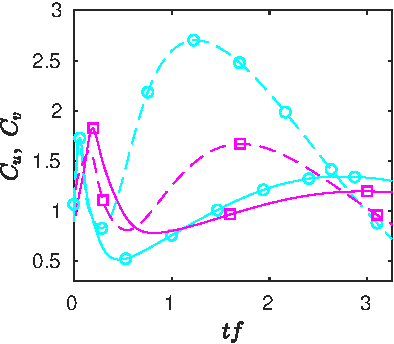
\includegraphics[width=2.3in,height=2in]{Cu_CV_combined-eps-converted-to}}
		\put(0.6,1.65){$\mathbf{(a)}$}
		%\put(1.2,0.01){\colorbox{white}{\makebox(0.75,0.15){}}}
	  \end{picture}
	\end{minipage}%
	\begin{minipage}{0.5\textwidth}
	\setlength{\unitlength}{1in}
	\begin{picture}(2.3,2)
		\put(0,0){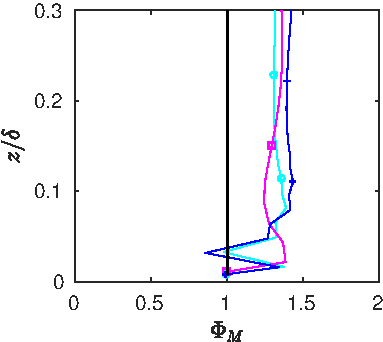
\includegraphics[width=2.3in,height=2in]{combined_phiM-eps-converted-to}}
		\put(0.6,1.65){$\mathbf{(b)}$}
		%\thicklines
        %\put(2.85,0.53){\line(0,1){1.42}}
	\end{picture}
	\end{minipage}
\caption{Measurement of unsteadiness in the mean flow and the profile of vertical gradient. (a). $C_u, C_v$ plotted against nondimensional time $tf$ for  EK10 and EK02. Solid lines correspond to $C_u$ and dotted lines to $C_v$. (b). Nondimensional vertical gradient of mean streamwise velocity, $\Phi_M=\kappa z u_*^{-1} d\left < \bar{u} \right >/dz$ plotted as a function of nondimensional height. Lines with markers $+$, $\smwhtcircle$, $\smwhtsquare$ correspond to $CHNL$, $EK10$, and $EK02$, respectively.  The solid black line corresponds to the classical log law expected to hold in the surface layer. }
\label{fig:cu-cv-phi_m}
\end{figure}

\graphicspath{{chap1Img/}}
\begin{figure}[htb]
	\begin{minipage}{0.5\textwidth}
	\setlength{\unitlength}{1in}
	  \begin{picture}(2.3,2)
		\put(0,0){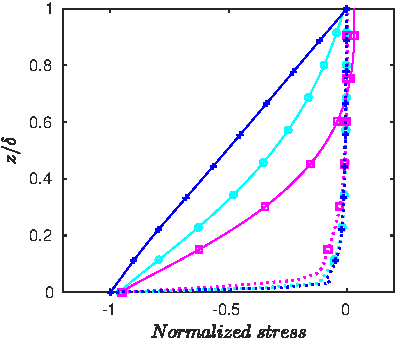
\includegraphics[width=2.3in,height=2in]{totalVerticalStress_uw_combined-eps-converted-to}}
		 \put(0.6,1.7){$(a)$}
		%\put(-0.1,2.5){$\mathbf{(a)}$}
		%\put(1.1,0.01){\colorbox{white}{\makebox(1.55,0.175){ $ \mathbf{({u'_{1}u'_{3}+ \tau_{13})}/u_*^{2}}$}}}		
		\thicklines
		%\put(2.844,0.47){\line(0,1){1.45}}
	  \end{picture}
	\end{minipage}%
	\begin{minipage}{0.5\textwidth}
	\setlength{\unitlength}{1in}
	\begin{picture}(2.3,2)
		\put(0,0){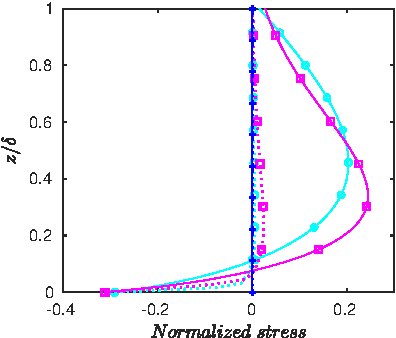
\includegraphics[width=2.3in,height=2in]{totalVerticalStress_vw_combined-eps-converted-to}}
		 \put(0.6,1.7){$(b)$}
		%\put(-0.1,2.5){$\mathbf{(b)}$}
		%\put(1.0,0.0){\colorbox{white}{\makebox(1.55,0.175){$ \mathbf{Normalized\ stress}$}}}
		\thicklines
     %   \put(2.85,0.47){\line(0,1){1.42}}
	\end{picture}
	\end{minipage}
\caption{Normalized vertical profiles of time and horizontally averaged resolved and SGS stresses. (a) $\left <\bar{u_1}'\bar{u_3}'+ \tau_{13}\right>$ and $\tau_{13}$ plotted as a function of height normalized by boundary layer height ($\delta$) for cases $EK10$, $EK02$, and $CHNL$. Solid lines correspond to $\left <\bar{u_1}'\bar{u_3}' + \tau_{13} \right >$ and dotted lines correspond to $\tau_{13}$. (b) $\left <\bar{u_2}'\bar{u_3}'+ \tau_{23}\right>$ and $\tau_{23}$ plotted as a function of normalized height for cases $EK10$, $EK02$, and $CHNL$. Solid lines correspond to $\left <\bar{u_2}'\bar{u_3}' + \tau_{23} \right >$ and dotted lines to $\tau_{23}$. Line types $-\smwhtcircle-$, $-\smwhtsquare-$ and $-+-$ correspond to $EK10$, $EK02$, and $CHNL$, respectively.}
\label{fig:uw-vw}
\end{figure}
\graphicspath{{chap1Img/}}
\begin{figure}
\setlength{\unitlength}{1in}
\begin{picture}(5,2)
\put(1,0){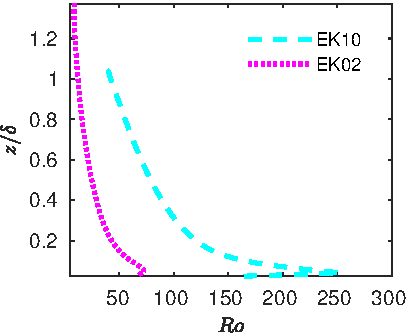
\includegraphics[width=2.3in,height=2in]{rossbyNo-eps-converted-to}}{}%
\end{picture}
\caption{Vertical Rossby number profile of $EK10$ and $EK02$ plotted as a function of normalized height.}
\label{fig:rossbyno}
\end{figure}


%-----------------------autocorrelation plot---------------------------------- -------
\graphicspath{{chap1Img/}}
\begin{figure}
\centering {
	\begin{minipage}{0.49\textwidth}
	  \setlength{\unitlength}{1in}
	  \begin{picture}(3,2.5)
		  \put(0,0.0){{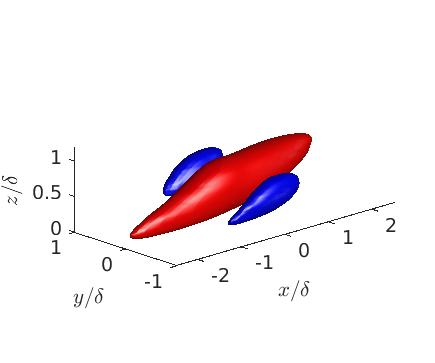
\includegraphics[width=3.0in,height=2.5in]{corr3d-with-midBL-chnl}}}{}% 
		  \put(0.75,1.78){$(a)$}
		\end{picture}
	\end{minipage}%
	\begin{minipage}{0.49\textwidth}
	\setlength{\unitlength}{1in}
	    \begin{picture}(2.3,2.5)
		    \put(0,0){{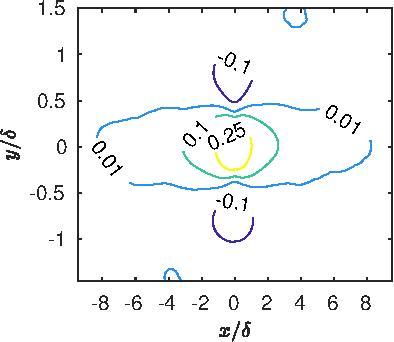
\includegraphics[width=2.3in,height=2in]{corr2d_z_delta_0d47_chnl-eps-converted-to}}}{}% 
		    \put(0.75,1.78){$(a')$}
		  \end{picture}
	\end{minipage}%	
	
	\begin{minipage}{0.49\textwidth}
	\setlength{\unitlength}{1in}
	  \begin{picture}(3,2.5)
		  \put(0,0){{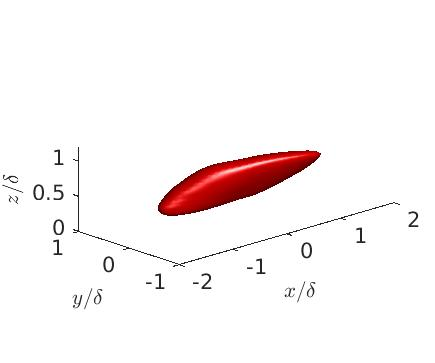
\includegraphics[width=3.0in,height=2.5in]{corr3d-with-midBL-ug10}}}{}% 
		  \put(0.75,1.78){$(b)$}
		\end{picture}
  \end{minipage}
  	\begin{minipage}{0.49\textwidth}
  	\setlength{\unitlength}{1in}
	  \begin{picture}(2.3,2.5)
		  \put(0,0){{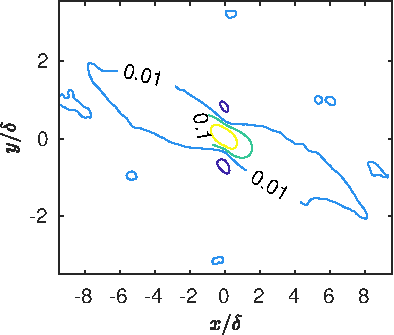
\includegraphics[width=2.3in,height=2in]{corr2d_z_delta_0d47_ek10-eps-converted-to}}}{}% 
		  \put(0.75,1.78){$(b')$}
		\end{picture}
  \end{minipage}	
  
	\begin{minipage}{0.49\textwidth}
	\setlength{\unitlength}{1in}
	  \begin{picture}(3,2.5)
		  \put(0,0){{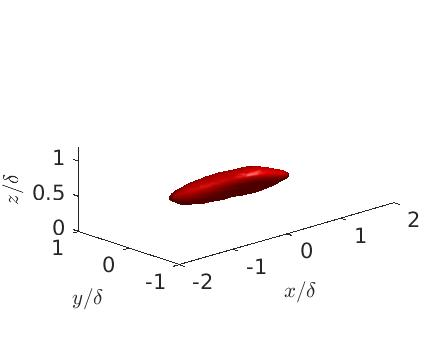
\includegraphics[width=3.0in,height=2.5in]{corr3d-with-midBL-ug02}}}{}% 
		  \put(0.75,1.78){$(c)$}
		\end{picture}
  \end{minipage}
  	\begin{minipage}{0.49\textwidth}
  	\setlength{\unitlength}{1in}
	  \begin{picture}(2.3,2.5)
		  \put(0,0){{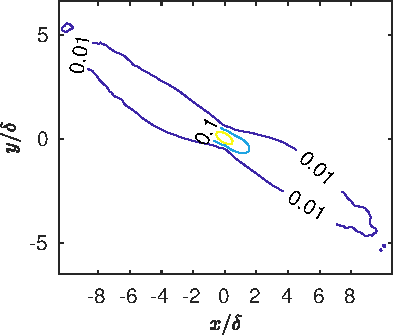
\includegraphics[width=2.3in,height=2in]{corr2d_z_delta_0d47_ek02-eps-converted-to}}}{}% 
		  \put(0.75,1.78){$(c')$}
		\end{picture}
  \end{minipage}  
}
\caption{Correlation of u-velocity component. $(a)$, $(b)$, $(c)$ show correlation of reference level $z/\delta=0.5$ with all other horizontal levels as defined by Eqn. \ref{eqn:3d_corr} for $CHNL$, $EK10$, and $EK02$, respectively. Red iso-surfaces denote correlation greater than or equal to $0.25$ and blue iso-surfaces show negative correlation, smaller or equal to $-0.15$.  $(a', b', c')$ show planar autocorrelation, $R_{uu}^{2D}$ of $CHNL$, $EK10$, and $EK02$ at $x_3=0.5\delta$, respectively.}
\label{fig:corr}
\end{figure}


\graphicspath{{chap1Img/}} 
\begin{figure}
\begin{minipage}{0.5\textwidth}%
  \setlength{\unitlength}{1in}
  \begin{picture}(2.3,2)
  \put(0,0){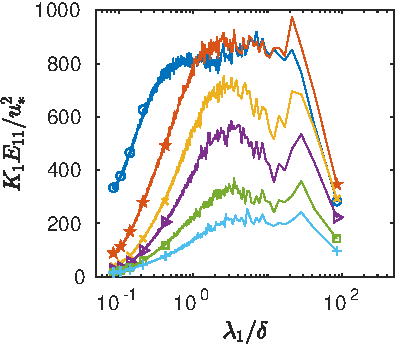
\includegraphics[width=2.3in,height=2in]{premult_u_spec_stream-wise-frame_chnl-eps-converted-to}}
  \put(0.76,1.7){$(a)$}
  \end{picture}%
\end{minipage}
\begin{minipage}{0.49\textwidth}%
  \setlength{\unitlength}{1in}
  \begin{picture}(2.3,2)
  \put(0,0){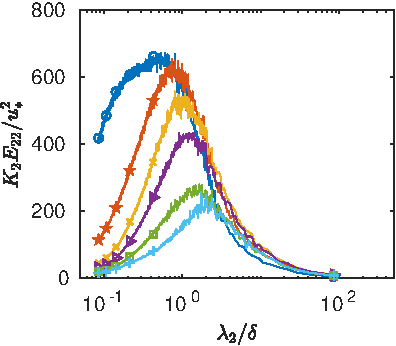
\includegraphics[width=2.3in,height=2in]{premult_v_spec_span-wise-frame_chnl-eps-converted-to}}
  \put(0.76,1.7){$(a')$}
  \end{picture}
\end{minipage}

\begin{minipage}{0.5\textwidth}%
  \setlength{\unitlength}{1in}
  \begin{picture}(2.3,2)
  \put(0,0){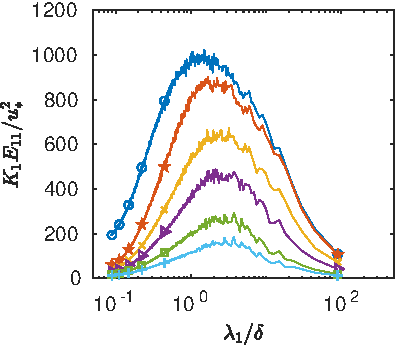
\includegraphics[width=2.3in,height=2in]{premult_u_spec_stream-wise-frame_ug10-eps-converted-to}}
  \put(0.76,1.7){$(b)$}
  \end{picture}
\end{minipage}%
\begin{minipage}{0.49\textwidth}
   \setlength{\unitlength}{1in}
  \begin{picture}(2.3,2)
  \put(0,0){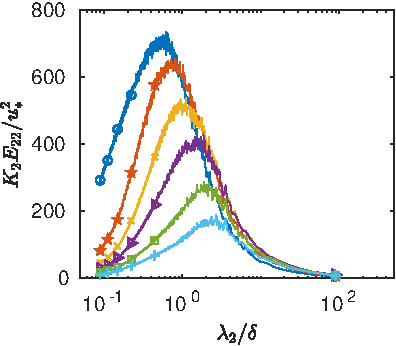
\includegraphics[width=2.3in,height=2in]{premult_v_spec_span-wise-frame_ug10-eps-converted-to}}
  \put(0.76,1.7){$(b')$}
  \end{picture}
\end{minipage}

\begin{minipage}{0.5\textwidth}%
  \setlength{\unitlength}{1in}
  \begin{picture}(2.3,2)
  \put(0,0){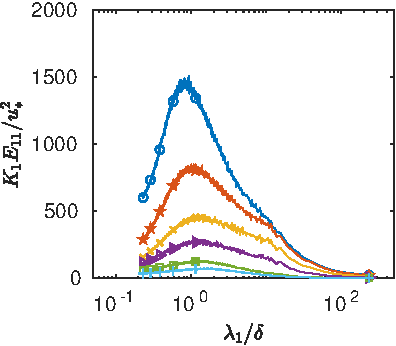
\includegraphics[width=2.3in,height=2in]{premult_u_spec_stream-wise-frame_ug2-eps-converted-to}}
  \put(0.76,1.7){$(c)$}
  \end{picture}
\end{minipage}%
\begin{minipage}{0.49\textwidth}%
   \setlength{\unitlength}{1in}
  \begin{picture}(2.3,2)
  \put(0,0){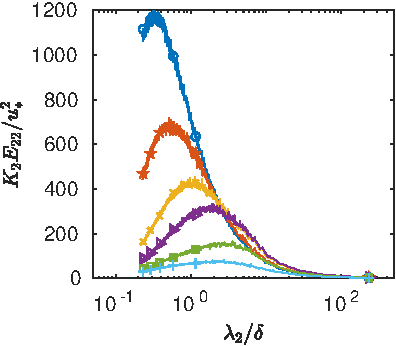
\includegraphics[width=2.3in,height=2in]{premult_v_spec_span-wise-frame_ug2-eps-converted-to}}
  \put(0.76,1.7){$(c')$}
  \end{picture}
\end{minipage}

\caption{Premultiplied velocity spectra against normalized wavelengths are shown for different cases. $(a)$, $(b)$, $(c)$ show spectra of the $u$-component of the velocity for $CHNL$, $EK10$, and $EK02$, respectively. $(a')$, $(b')$, $(c')$ show spectra of the $v$-component of the velocity for $CHNL$, $EK10$, and $EK02$, respectively. Curves marked with ($\smwhtcircle, \smwhitestar, \times, {\triangledown}, \smwhtsquare, +$) correspond to heights $x_3/\delta = (0.06,\ 0.15, \ 0.30,\ 0.45, \ 0.71, \ 0.90)\pm 0.01$, respectively.}
\label{spec_pre_spec}
 \end{figure}
 
 
 \graphicspath{{chap1Img/}}
\begin{figure}[htb]
	\begin{minipage}{0.5\textwidth}
	\setlength{\unitlength}{1in}
	  \begin{picture}(2.3,2)
		\put(0,0){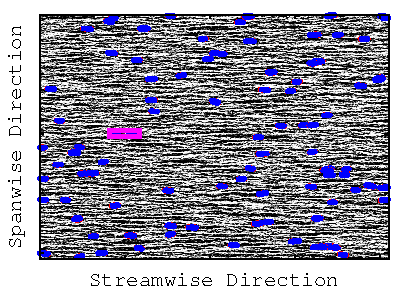
\includegraphics[width=2.3in,height=2in]{chnl_bin_lowMom-eps-converted-to}}
		%\put(-0.1,2.5){$\mathbf{(a)}$}
		\put(0.5,-0.01){\colorbox{white}{\makebox(1.55,0.175){ $ {Streamwise\ direction}$ }}}	
		\put(-0.15,-0.1){\colorbox{white}{\makebox(0.25,2.175){\rotatebox{90}{$ {Spanwise\ direction}$}}}}	
	  \end{picture}
	\end{minipage}%
	\begin{minipage}{0.5\textwidth}
	\setlength{\unitlength}{1in}
	\begin{picture}(2.3,2)
		\put(0,0){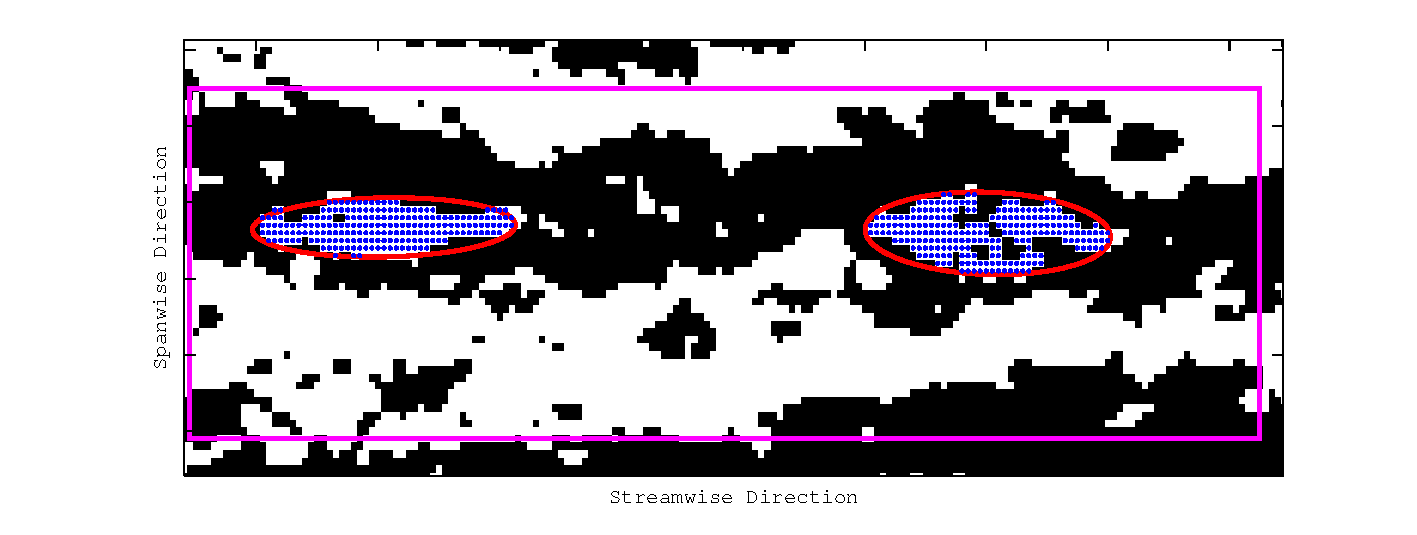
\includegraphics[width=2.3in,height=2.05in]{cropped-eps-converted-to}}
		\put(0.5,-0.01){\colorbox{white}{\makebox(1.55,0.175){ $ {Streamwise\ direction}$ }}}	
		\put(-0.0005,-0.1){\colorbox{white}{\makebox(0.2,2.175){\rotatebox{90}{${Spanwise\ direction}$}}}}		
	\end{picture}
	\end{minipage}
\caption{Identification of VLSMs. (Left) For the $CHNL$ case, a cropped binarized negative $u'$ velocity field image is shown, which is overlayed with detected elliptical coherent structures with a range of major axis length lengths, $\delta-10\delta$. (Right) Zoomed-in two detected structures with interior points painted in blue where average shear stresses were calculated are shown. Horizontal and vertical axes are aligned with streamwise and spanwise directions, respectively} 
\label{area_binarized_vel_image}
\end{figure}
\graphicspath{{chap1Img/}}
\begin{figure}
\centering {
	\begin{minipage}{0.49\textwidth}
	  \setlength{\unitlength}{1in}
	  \begin{picture}(2.3,2.08)
		  \put(0,0){{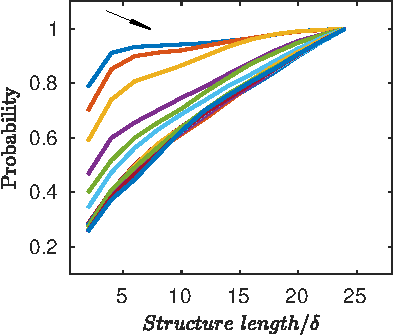
\includegraphics[width=2.3in,height=2in]{struclen_cdf_chnl-eps-converted-to}}}{}% 
		  \put(2.2,0.55){$(a)$}
		\end{picture}
	\end{minipage}%
	\begin{minipage}{0.49\textwidth}
	\setlength{\unitlength}{1in}
	    \begin{picture}(2.3,2.08)
		    \put(0,0){{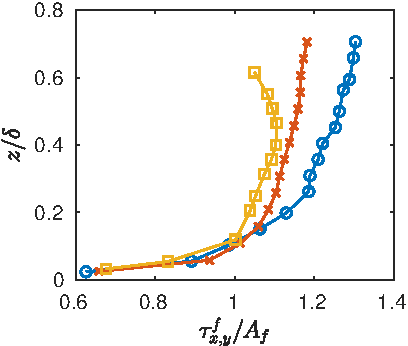
\includegraphics[width=2.3in,height=2.06in]{flux_area_frac_ratio_all_band-eps-converted-to}}}{}% 
		    \put(2.2,0.55){$(d)$}
		  \end{picture}
	\end{minipage}%	
	
	\begin{minipage}{0.49\textwidth}
	\setlength{\unitlength}{1in}
	  \begin{picture}(2.3,2.08)
		  \put(0,0){{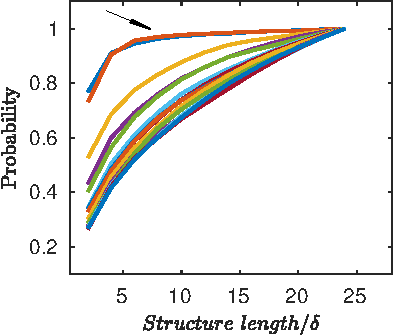
\includegraphics[width=2.3in,height=2in]{struclen_cdf_ek10-eps-converted-to}}}{}% 
		  \put(2.2,0.55){$(b)$}
		\end{picture}
  \end{minipage}
  	\begin{minipage}{0.49\textwidth}
  	\setlength{\unitlength}{1in}
	  \begin{picture}(2.3,2.08)
		  \put(0,0){{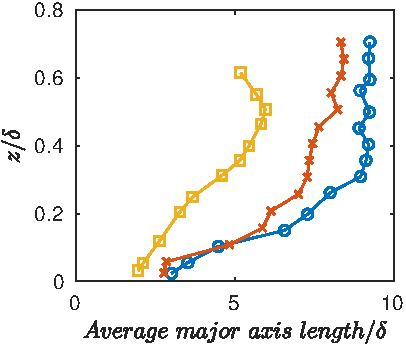
\includegraphics[width=2.3in,height=2.06in]{avg_majorAxisLength_all_band-eps-converted-to}}}{}% 
		  \put(2.2,0.55){$(e)$}
		\end{picture}
  \end{minipage}	
  
	\begin{minipage}{0.49\textwidth}
	\setlength{\unitlength}{1in}
	  \begin{picture}(2.3,2.08)
		  \put(0,0){{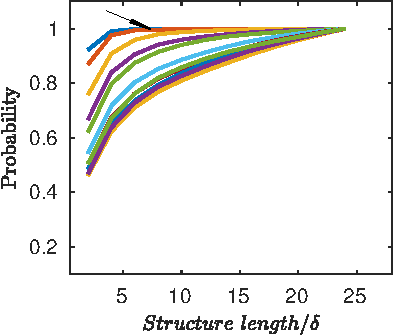
\includegraphics[width=2.3in,height=2in]{struclen_cdf_ek02-eps-converted-to}}}{}% 
		  \put(2.2,0.55){$(c)$}
		\end{picture}
  \end{minipage}
  	\begin{minipage}{0.49\textwidth}
  	\setlength{\unitlength}{1in}
	  \begin{picture}(2.3,2.08)
		  \put(0,0){{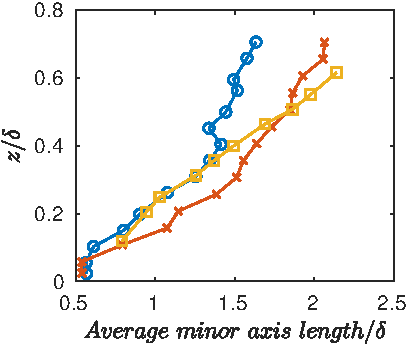
\includegraphics[width=2.3in,height=2.06in]{avg_minorAxisLength_all_band-eps-converted-to}}}{}% 
		  \put(2.2,0.55){$(f)$}
		\end{picture}
  \end{minipage}  
}
\caption{Cumulative density function of coherent structure lengths, their aggregate contribution to shear stress as functions of height, and their average lengths. The left panel shows cumulative density function of the structure lengths detected in the range $\delta-25\delta$ for $CHNL$ (a), $EK10$ (b), and $EK02$ (c) cases. The arrows point to the direction of increasing distance from the surface. The panel on the right-hand side shows the ratio (d) $\tau_{x,y}^f/A_f$ plotted for different wall-normal locations of all cases. (e) shows the mean length of major axes for all structures detected  and (f) shows the mean minor axes lengths. Here ($-\smwhtcircle-$) represents $CHNL$, ($-\times-$) represents $EK10$, and ($-\smwhtsquare-$) represents $EK02$.}
\label{fig:stress_cont_cdf_length}
\end{figure} 

\graphicspath{{chap1Img/}}
\begin{figure}
\centering {
	\begin{minipage}{0.49\textwidth}
	  \setlength{\unitlength}{1in}
	  \begin{picture}(2.9,2)
		  \put(0,0){{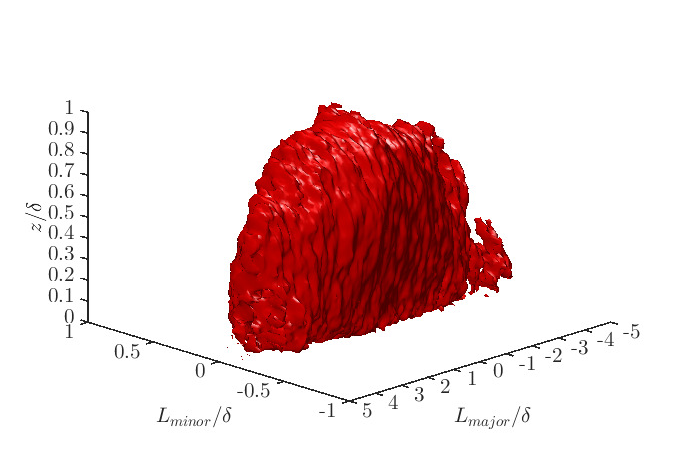
\includegraphics[width=2.89in,height=2in]{vlsm_chnl}}}{}% 
		  \put(0.75,1.5){$(a)$}
		\end{picture}
	\end{minipage}%
	\begin{minipage}{0.48\textwidth}
    	\setlength{\unitlength}{1in}
	    \begin{picture}(2.3,2)
		    \put(0,0){{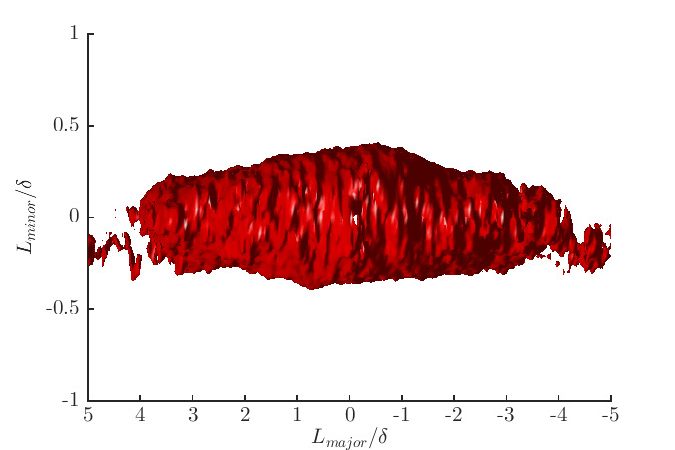
\includegraphics[width=2.3in,height=2in]{vlsm_chnl_topView}}}{}% 
		    \put(0.75,1.5){$(a')$}
		  \end{picture}
	\end{minipage}%	
	
	\begin{minipage}{0.49\textwidth}
	 \setlength{\unitlength}{1in}
	  \begin{picture}(2.9,2)
		  \put(0,0){{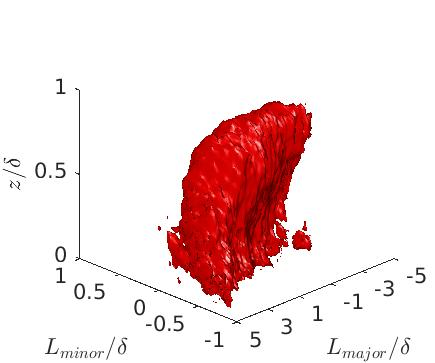
\includegraphics[width=2.89in,height=2in]{vlsm_ek10}}}{}% 
		  \put(0.75,1.5){$(b)$}
		\end{picture}
  \end{minipage}
  	\begin{minipage}{0.49\textwidth}
  	\setlength{\unitlength}{1in}
	  \begin{picture}(2.3,2)
		  \put(0,0){{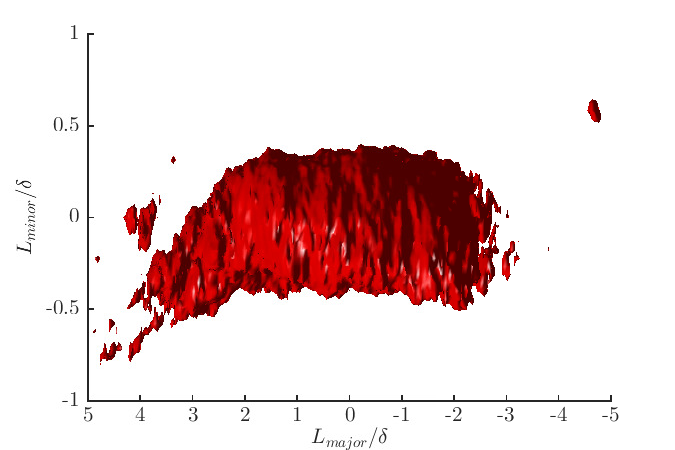
\includegraphics[width=2.3in,height=2in]{vlsm_ek10_topView}}}{}% 
		  \put(0.75,1.5){$(b')$}
		\end{picture}
  \end{minipage}	
  
	\begin{minipage}{0.49\textwidth}
	\setlength{\unitlength}{1in}
	  \begin{picture}(2.9,2)
		  \put(0,0){{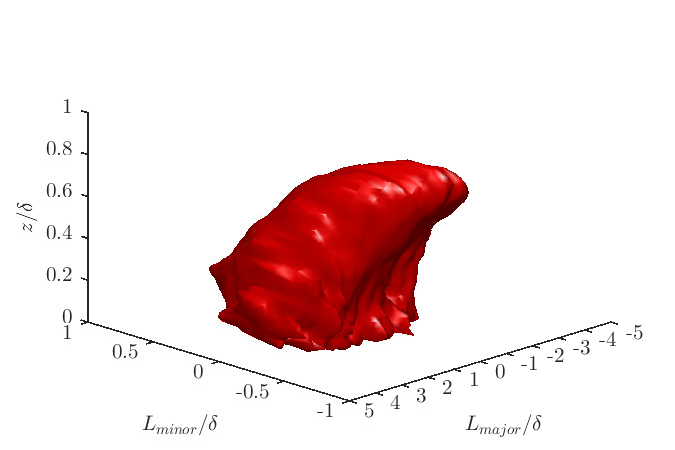
\includegraphics[width=2.89in,height=2in]{vlsm_ek02}}}{}% 
		  \put(.75,1.5){$(c)$}
		\end{picture}
  \end{minipage}
  	\begin{minipage}{0.49\textwidth}
  	\setlength{\unitlength}{1in}
	  \begin{picture}(2.3,2)
		  \put(0,0){{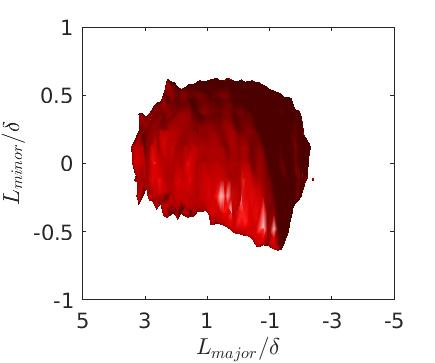
\includegraphics[width=2.3in,height=2in]{vlsm_ek02_topView}}}{}% 
		  \put(0.75,1.5){$(c')$}
		\end{picture}
  \end{minipage}  
}
\caption{3D structure of VLSMs. $(a)$, $(b)$, $(c)$ show the average 3D structures projected from detected 2D transects at the height of the first vertical grid point for the $CHNL$, $EK10$, and $EK02$ cases, respectively. $(a')$, $(b')$, $(c')$ show the top view of the same 3D structures as shown on the left panels. Iso surfaces enclose values less than $\left < u\right >-1.5\sigma_{u}$ }
\label{fig:vlsm-3d}
\end{figure} 


%%% -*-LaTeX-*-

\chapter{Modulation by very large scales and scale-scale energy transfer to and from large-scale motion}\label{chap:chap2}
The existence of large and very large scale motions (LSMs/VLSMs) in the ABL was reported in previous studies. It was also reported from experimental studies that the large-scale motions modulate the small scales. However, the possible influence of large scales over small scales due to nonlocal turbulent kinetic energy ($tke$) exchange was not examined. Also, the mechanism of spatial development of VLSMs was speculated mostly from visualization of flow features and was not examined in the light of $tke$ exchange. It can be expected that the formation mechanism of LSMs and VLSMs will have some signatures in the energy exchange process between individual scales as governed by the nonlinear term of the Navier-Stokes equations. Here, the modulation effect of large scales on smaller scales is interrogated in the simulated flow fields and the energy exchange between different scales has been explored in the wavelet domain. It has been observed that the energy exchange is not influenced by the presence of VLSMs or different forcing conditions in the examined cases and $tke$ exchange is predominantly local. However, support has been found from the interscale energy exchange process in favour of the hypothesis that LSMs concatenate to give rise to VLSMs.


\section{Introduction}

Many studies have confirmed the existence of Large-Scale and Very Large-Scale Motions (LSMs and VLSMs) throughout the boundary layer in pipe \citep{monty_jfm_07,guala_adrian_jfm2006,baltzer_jfm_13}, channel \citep{monty_jfm_07,balakumar_adrian_ptrs_07,lee_sung_jfm_14,hutchins_marusic_jfm2007,fang2015blm}, and zero pressure gradient boundary layer flows \citep{balakumar_adrian_ptrs_07,Lee_sung_jfm11,hutchins_marusic_jfm2007}. Flow structures corresponding to LSMs and VLSMs can be visually identified in an instantaneous flow field as long streaks of low momentum primarily oriented along the streamwise direction and flanked by similarly shaped high-momentum regions on either side. These structures scale with outer length scales $\delta$, where $\delta$ denotes boundary layer depth, channel half height, pipe radius, etc. depending upon the flow. Monty et al. \citep{monty_jfm_07} measured streamwise velocity with hot wire rakes in a pipe and in a channel and reconstructed the spatial velocity field using Taylor's frozen turbulence hypothesis to visually identify VLSMs. In their study, they observed VLSMs of the order of $25\delta$ in the log layer. Using a similar hot wire apparatus, \citet{hutchins_marusic_jfm2007} also visually identified VLSMs in the log layer of a wind tunnel boundary layer and reported length scales to be found of the order of $20\delta$. They also reported the existence of VLSMs in the buffer layer through their studies of DNS data of channel flow and speculated that correlations likely exist between log-layer-VLSMs and buffer-layer-VLSMs. Using stereoscopic particle image velocimetry data in conjunction with the application of Taylor's frozen turbulence hypothesis, \citet{dennis_nickels_jfm2011} constructed a 3D velocity field from data collected in a water tunnel and showed the 3D structure of VLSMs through a series of iso-surface plots. VLSMs were shown to be low-speed (or high-speed) turbulent bulges inclined with respect to the wall and mainly elongated in the streamwise direction that extend from the wall towards the outer region in the wall-normal direction \citep{dennis_nickels_jfm2011}. Other studies have come to similar conclusions \citep{chung_jfm_10_large,kerherv_roux_etfs_2017}. 

Studies on VLSMs and LSMs are plagued by a lack of an objective definition of these large-scale motions. All visual detection procedures are subjective in nature and a threshold value has to be chosen while visualizing low-momentum or high-momentum regions. \citet{dennis_nickels_jfm2011} appropriately pointed out that choosing a higher threshold may result in underestimation of length of these long structures while inappropriate filtering may smooth away small-scale structures and join smaller structures to give an impression of a single large-scale structure. A more objective definition or detection criteria of the length scales of VLSMs comes from premultiplied 1D spectra of the streamwise velocity component. A bimodal distribution of energy is observed in the premultiplied spectra, where the low wavenumber peak corresponds to VLSMs and the most energy containing relatively large wavenumber mode before a sharp fall-off corresponds to LSMs. This observation of the bimodal distribution has been used to distinguish the two length scales, i.e., LSM and VLSM \citep{kim_adrian_pof99,balakumar_adrian_ptrs_07,guala_adrian_jfm2006}. However, this scale identification from 1D spectra is not devoid of pitfalls. \citet{hutchins_marusic_jfm2007}  pointed out that the meandering nature of the VLSM can cause a shift of the energy peak in premultiplied spectra to shorter wavelengths. Also the approach of extracting a dominant wavelength from energy spectra of the streamwise velocity component to identify VLSMs has an inherent assumption \citep{baltzer_jfm_13} that spatially a low-momentum region would be in immediate vicinity of a high-momentum region of similar length scale in the streamwise direction and, since a VLSM structure represents only a half cycle of a sinusoidal function, the low wavenumber peak in spectra would be indicative of twice the length scale of the VLSM. The issues have been reflected as discrepancies on reported length scales of VLSMs from the premultiplied spectra and visualisation methods. In logarithmic regions of channel and boundary layer flows energy peaks corresponding to wavelengths $7.5\delta$ and $5\delta$ have been reported \citep{balakumar_adrian_ptrs_07}, whereas VLSM length scales of the order of $10\delta$ have been reported from visualizations in both cases \citep{Lee_sung_jfm11,lee_sung_jfm_14,hutchins_marusic_jfm2007}. We feel the need for an alternative approach to asses the importance of VLSMs along with the identification of the probable length scale. 

The wavelet framework offers an alternative approach to look at scale-dependent energy transfers and deduce the important length scales of turbulent dynamics. The most pursued way of analysing scale-to-scale energy transfer involves studying triadic interaction between scales coupled through the nonlinear term in the Fourier domain. Fundamentally, this approach is decoupled from spatial-transport phenomena and the analysis can assess interactions only in a global sense from a spatial point of view due to the nonlocality of sinusoidal functions. The other approach is to study the interaction among scales in both physical space and length scale  space utilising structure functions. In this approach, one attempts to analyze the terms of a diagnostic equation of the turbulent kinetic energy ($tke$) budget derived from the second-order structure function as outlined by Hill \citep{hill_jfm2002}. Marati et al. \citep{marati_jfm_2004} studied an inhomogeneous wall bounded flow using the formulation sketched by Hill \citep{hill_jfm2002}. However, this approach is limited in exploring the length scales bounded by integral-length scales since, structure functions lose physical significance when the auto-correlation drops to a nonsignificant value. 

In this study, we focus on scale-scale energy transfers associated with VLSMs in the atmospheric boundary layer (ABL). The ABL is distinguished from laboratory-scale flows due to the presence of a diurnally varying buoyancy  force and the Coriolis force. Previous studies analyzed length scales of LSMs and VLSMs and the probable mechanisms of their organization, but the question whether weak rotation of the reference frame and atmospheric stability (buoyancy) affects the length scales and organization of these structures remained unanswered. In order to study the effect of Coriolis force on VLSMs, a very large domain of the order of $100\delta$ is desirable given that VLSMs can span a length of $10\delta$. Such requirements poses a fundamental predicament to the DNS approach. Multipoint experimental measurements over such a large domain is also prohibitive, if not impossible. The most practical solution is offered by the large eddy simulation (LES) technique that was used for this study. In order to study two different regimes of large scales and to identify and differentiate their dynamics and significance, a boundary must be delineated between the two regimes of large scales, i.e., LSM and VLSM. We assume that the demarcation scale between LSMs and VLSMs is $\pi\delta$ corresponding to $k_x\delta = 2$ following \citet{guala_adrian_jfm2006}. Since the subjects of this study are VLSMs and LSMs along with the impact of the earth's rotation on them, simulation of very large flow fields was required. To properly resolve length scales as large as $20\delta$,  we chose a domain large enough that these large scales were properly captured as structures advecting freely through the flow field. The possibility that LSMs and VLSMs  interact with smaller scales nonlocally is also explored.  First, we briefly describe the simulation methods and basic flow properties (Sec. \ref{sec:LES_chap2}) and continue with an assessment of the modulating influence of VLSMs on smaller scales as observed from our numerical data set (Sec. \ref{Modulation_VLSMs}).  Section \ref{Analysis of inter-scale energy transfer in wavelet domain} presents the results obtained from analysis of interscale energy transfers in the wavelet domain with a brief introduction to the wavelet method and relevant discussion on LSMs and VLSMs. Finally, we wrap up with a discussion on probable mechanics of developing VLSMs from smaller scale motions. 

\section{Large Eddy Simulations}
\label{sec:LES_chap2}
Three different flow cases were simulated for this study designated as $CHNL$, $EK10$, and $EK02$. $CHNL$ is a classic high Reynold's number channel flow simulation over a large horizontal domain where the flow is sustained by a mean pressure gradient applied across the streamwise ($x$) direction. The mean flow velocity vector in this case points to x-direction. Turbulence is fed off the mean velocity due to instabilities \citep{landahl_christensen_book_92}. The velocity component that contributes most to the turbulent kinetic energy ($tke$) is the x-component of the velocity ($u_1$) and contribution of the spanwise velocity ($u_2$) to the $tke$ is insignificant, unlike in $EK10$ and $EK02$. $EK10$ and $EK02$ are simulations of Ekman layer flows with geostrophic wind velocities ($U_g$) of $10$ m/s and $2$ m/s, respectively (Table \ref{tab:sim_param}). A geostrophic wind condition refers to the balance between the Coriolis force and the mean pressure gradient ($\rho^{-1}\frac{\partial \left < p \right >}{\partial x_i} = f_c\epsilon_{ij3}\tilde{u}_j$) under horizontal homogeneity, and a zero wall-normal stress boundary conditions at the top edge of the BL. Consequently, at the top of the BL, the momentum equation for the z-direction reduces to, $\frac{\partial \left < p \right >}{\partial z} = 0$. In terms of forcing, the key difference between the simulated channel and Ekman cases in this study is that, in $CHNL$, a constant $\left < \rho^{-1} \frac{\partial P}{\partial x} \right >$ sustains the flow while in $EK10$ and $EK02$ a constant $\left < \rho^{-1}\frac{\partial p }{\partial y} \right >  = -f_c U_g$ is acting on the flow, where $f_c$ is the Coriolis parameter. Effectively, the Ekman layer flows are constant pressure gradient flows in a rotating frame of reference. 

All three simulations were carried out in a LES framework where the spatially filtered Navier-Stokes equations for an incompressible flow in the ABL were solved in conjunction with a subgrid-scale stress model. The model equations can be expressed as: 
\begin{align}
    \frac{\partial \tilde{u}_i}{\partial x_{i}} &= 0, \\
    \frac{\partial \tilde{u}_i}{\partial t}+ \frac{\partial \tilde{u}_i\tilde{u}_j}{\partial x_{j}}  &= \frac{-\partial \tilde{p^*}}{\partial x_i}-\frac{\partial \tau_{ij}}{\partial x_j}+ f_{c}\epsilon_{ij3}\tilde{u}_{j},   
\label{eqn:les_eqn}    
\end{align}
\noindent where $i={1,2,3}$ corresponds to $x,y,z$ directions, respectively, ${\tilde{}}$ denotes spatial filtering, $\tilde{u}_i$ denotes the spatially filtered velocity component in the $i$-direction, $\tilde{p^*}=\frac{1}{\rho} \tilde{p}+\frac{1}{3}\tau_{kk}$ is the modified, filtered pressure, the Coriolis parameter has a prescribed value of $10^{-4}$, and $\tau_{ij}$ is the modelled subgrid-scale stress tensor defined as $\tau_{ij}=\widetilde{u_i u_j}-\tilde{u}_i\tilde{u}_j$. $\tau_{ij}$ was modeled with a scale-dependent Lagrangian dynamic subgrid-scale model. Further details of the subgrid-scale model can be found in \citet{stoll_wrr_2006}. The LES code used in this study is pseudo-spectral in nature and uses a Cartesian, staggered grid. Horizontal derivatives are calculated in spectral space while in the surface-normal direction, a second-order-accurate finite-difference approximation is used. Dealiasing was applied through the $3/2$ rule, the lateral boundary conditions were periodic, and the top of the domain utilized a stress free condition, i.e., $\partial\tilde{u}_1/\partial x_3 = \partial \tilde{u}_2/\partial x_3=0$ and the velocity fields were kept divergence free by pressure-correction through the solution of the Poisson equation for the pressure.  All three simulations were run for long enough time to reach a quasi-steady condition. At the wall, instantaneous surface shear stresses, $\tau_{i3,s}(x,y,t)$, were needed as part of the boundary condition, and were computed as a function of the resolved scale velocities $\tilde{u}_1$ and $\tilde{u}_2$ at the lowest vertical nodes at a height of $\Delta_z/2$. This was done using Monin-Obukhov similarity theory as follows:
\begin{align}
\tau_{i3,s}(x,y,t) = -\left [ \frac{\tilde{u}_r(x,y,z,t)\kappa}{\ln(z/z_o)} \right ]^2\frac{\tilde{u}_i(x,y,z,t)}{\tilde{u}_r(x,y,z,t)}, 
\end{align}
\noindent where $\kappa$ is the von K\'arman constant ($=0.4$) and $z_o$ is the local aerodynamic roughness length which was assumed to be $0.1$ m in the simulated cases. The code has been used to simulate the ABL under a variety of different forcing conditions \citep[e.g.,][]{stoll_jas_2009,bailey_blm_2013,miller_blm_2013} and to examine the structure and evolution of turbulent motions \citep[e.g.,][]{bailey_ae_2014,bailey_jfm_2016}.  Its excellent representation of SGS momentum fluxes \citep{stoll_wrr_2006} makes it ideal for an examination of large-scale velocity-field dynamics. In the horizontal directions ($x$, $y$), the extents of the domains ($L_x$, $L_y$) were $128$ Km and in the vertical direction (z), $1.5$, $1.5$, and $0.75$ Km for $CHNL$, $EK10$, and $EK02$, respectively (Table \ref{tab:sim_param}).  To decouple the effect of the Coriolis force from other typical atmospheric conditions such as buoyancy, neutral atmospheric conditions were assumed in all three cases and the effects of rotation were subsequently evaluated. By varying the geostrophic wind velocity, different degrees of rotational effects were observed. 

The filter scales $\Delta_x$ and $\Delta_y$ were the same in the horizontal directions $x$ and $y$, respectively. We took the filtered equations and decomposed the dependent variables further into horizontally  averaged ($\left< \zeta \right>$) and fluctuating components ($\zeta\prime$), where $\zeta$ stands for any of the dependent variables. For convenience, the tilde will be dropped and all dependent variables will be understood as spatially filtered quantities. With the proposed decomposition and under the assumption that this horizontal averaging over statistically independent frames conforms to Reynold's averaging, the transport equation for the turbulent kinetic energy ($q$) takes the following form:
\begin{align}
u_3^\prime u_i^\prime \frac{\partial \left< u_i \right>}{\partial x_3}+[\left< u_j\right>\frac{\partial q}{\partial x_j}+u_j^\prime\frac{\partial q}{\partial x_j}+\frac{\partial }{\partial x_j}(u_i^\prime \tau_{ij}^\prime)]+u_i^\prime\frac{\partial p^\prime}{\partial x_i}+ u_i^\prime \frac{\partial \left < p \right >}{\partial x_i}+u_i^\prime\frac{\partial \left < \tau_{i3} \right >}{\partial x_3}-\tau_{ij}^\prime s_{ij}^\prime =0,
\label{eqn:tke_horz_avg}
\end{align}
\noindent where, $q=\frac{1}{2}u^{\prime}_i u^{\prime}_i$ and $s_{ij}'=\frac{1}{2}(\frac{\partial u_{i}'}{\partial x_j}+\frac{\partial u_{j}'}{\partial x_i})$.
In Equation \ref{eqn:tke_horz_avg}, the first term on the left-hand side denotes production of $tke$ by mean shear, the second term captures the spatial redistribution of $tke$ by the mean flow and turbulence, and the third and fourth terms denote velocity and pressure correlation.  The fifth term stands for redistribution of $tke$ by horizontally averaged subgrid-scale turbulence, and the last term denotes subgrid-scale dissipation by turbulent motions. Although, this equation of $tke$ transport will not be directly analysed in this study, it will serve as a guidepost for the inter-scale energy transfer analysis. In this study a scale dependent version of the combined terms ($-\frac{\partial }{\partial x_i}\left< p^\prime u^\prime\right>-u_j^\prime\frac{\partial \left< q\right>}{\partial x_j}-\frac{\partial}{\partial x_j}\left< u_i^\prime\tau_{ij}^\prime \right>+\left< \tau_{ij}^\prime s_{ij}^\prime\right>$) was analysed via a discrete wavelet framework. Before analysis of the interscale energy exchange, the characteristics of VLSMs are examined to confirm that the same modulating characteristics of VLSMs are observed in simulated flows as was observed in experimental analysis. 

\section{Modulation of Small Scale Fluctuations by VLSMs}
\label{Modulation_VLSMs}

One of the most important identified features of VLSMs is their modulating influence on small scales. Although the precise mechanism of how this modulation takes place has not been definitely identified, through statistical analysis of small-scale fluctuations within an envelope of large-scale fluctuations, the influence can be verified and quantified. \citet{MATHIS2009} conducted tests on the modulating influence of VLSMs on small scales from multipoint measurements in the boundary layer. This was done by isolating the low-frequency envelope of high-frequency (small scale) fluctuations with an application of the Hilbert Transformation and correlating the filtered envelope with the appropriately matched VLSM signal in the near-wall region. A clear signature of long wavelength motions in the log layer modulating smaller scale motions in the roughness sublayer was shown. \citet{Bernardini2011} expanded upon the analysis of \citet{MATHIS2009} and calculated two-point correlations between the small wavenumber envelope of high-wavenumber fluctuations and large-scale fluctuations to demonstrate the appearance of a secondary peak in the amplitude-modulation covariance map. The secondary peak corresponded to long wavelengths and the findings solidified the basic conclusions of \citet{MATHIS2009} and \citet{ganapathi_jfm_2012_modulation}, hereafter referred to as GH12.  GH12 also looked into the amplitude modulation imparted by VLSMs in a high Reynolds number wind tunnel boundary layer utilizing a traversing hot-wire probe. A conditional analysis of small-scale motions as reported in GH12 proved that the amplitude, frequency, and phase of small-scale fluctuations are linked to the same variables of large-scale fluctuations. We adopted the analysis method of GH12 and explored the modulating effect of large-scale motions for the simulation data sets.  Results have been compared with that of GH12 to verify whether LSMs and VLSMs, as detected in the simulation data sets, exhibit similar effects.  For the sake of completeness, a brief description of the analysis is furnished here. For a complete description of the methods, GH12 should be consulted where a descriptive illustration is also presented. The key difference from the analysis of GH12 is that we analyze spatial data whereas, in GH12, the analysis was done on time-series data. To keep the analysis in line with a point measurement of a time series, we treat each streamwise row of the $u_{1}$-component of the velocity and turbulent stress ($u_{1}^{\prime} u_{3}^{\prime}$) as a single data series. Thus, on the $2048 \times 2048$ horizontal grid used here, we get 2048 independent data series at each wall-normal location on the simulation grid.  Four independent instantaneous snapshots of the flow field were taken for each case, thus providing a total of 8192 data sets on each horizontal plane. A brief description of the procedure is summarized below:
\begin{enumerate}[(i)]
\item The fluctuating streamwise velocity component ($u_{1}^\prime(z)$) was separated by subtracting the horizontally averaged velocity ($\left< u_{1}(z)\right>$) from each wall-normal plane from the instantaneous velocity fields.
\item The large-scale component of the fluctuating velocity field ($u_L(z)$) was obtained by filtering $u^\prime(z)$ with a spectral cut-off filter where the cut-off wavelength was $2\delta$ (the red smooth line as shown in Fig. \ref{fig:modulation}). The small-scale fluctuating component was obtained as: $u_s(z)=u^\prime(z)-u_L(z)$ (the cyan dotted line in Fig. \ref{fig:modulation}).
\item In each data, set the series of $u_s(z)$ and $u_L(z)$ were divided into segments of length $2\delta$. Similar segmentation was applied to the turbulent stress ($u_{1}^\prime u_{3}^\prime(z)$) series. Statistics in each individual segment were linked to the representative large-scale fluctuation values. 
\item Large-scale fluctuations were then categorized by a binning process based on the centre value of $u_L(z)$ from each segment of length $2\delta$ as described in step (iii) and as shown with a hypothetical binning in Fig. \ref{fig:modulation}. This process links each individual segment of small-scale data to a $u_L(z)$ bin. In other words, this process gives statistics of small scales conditioned on $u_L(z)$. The number of occurrences of $u_L(z)$ in each bin $N[u_L(z)]$ was counted for all data sets.    
\item In each segment of small scales ($u_s$), the following statistics were calculated:
 \begin{enumerate}[(1)]
    \item The relative variance of the small scales $\Delta u_s^2(u_L,z)$ as: 
    \begin{align}
        \Delta \left < u_s^{2+}\right > =\frac{\left < u_s^2(u_L,z)\right >_S-\left < u_s^2(u_L=0,z)\right >_S}{\left < u_s^2(u_L=0,z)\right >_S} \times 100,
    \label{eq:relative_var_us2}    
    \end{align}
    where $\left < u_s^2(u_L,z) \right >_S = \frac{\sum u_s^2(z)|_{u_L(z)}}{N[u_L(z)]}$ and $\left < u_s^2(u_L=0,z)\right >_S$ denotes $\left < u_s^2(u_L,z) \right >_S$ corresponding to the $u_L=0$ bin.
    \item The average wavenumber of the small-scale fluctuation. This was calculated by counting the number of zero-crossings ($N_m$) and then dividing by 2 ($N_m/2$). Finally, a mean representative wavenumber was calculated as:
    \begin{align}
        \left< k_x|u_L \right> = \frac{\sum k_x(z)}{N[u_L(z)]},
        \label{eq:kx_uL}
    \end{align} 
    where $\sum k_x$ refers to the summation of the average $k_x$ values of all data sets corresponding to an individual $u_L(z)$ bin on a horizontal plane. 
    \item At different surface-parallel planes the mean $\left < u_{1}^\prime u_{3}^\prime\right >$ and variance $\sigma^2_{u_{1}^\prime u_{3}^\prime}$ (of the wall-normal stress ($u_{1}^\prime u_{3}^\prime$)) for each bin were calculated. Finally, a combined mean $\left < u_{1}^\prime u_{3}^\prime \right >_{u_L}$ and a pooled standard deviation ($\sigma^{u_{1}^\prime u_{3}^\prime}_{u_L}$) corresponding to each $u_L$ bin was calculated as: 
    \begin{align}
      \left < u_{1}'u_{3}' \right >_{u_L} = \frac{\sum \left < u_{1}'u_{3}'\right > N_S}{\sum N_S} \ \text{and}
      \label{eq:u'w'_mean}
    \end{align}
    \begin{align}
      \sigma^{u_{1}'u_{3}'}_{u_L} = \sqrt \frac{\sum [\sigma^2_{u_{1}'u_{3}'} + (\left < u_{1}'u_{3}'\right > -\frac{\sum \left < u_{1}'u_{3}'\right >}{\sum N_S})^2 N_S]}{\sum N_S}
     \label{eq:std_uw} 
    \end{align}    
    where the summation ($\sum $) was taken over all segments of the data series on a horizontal plane, corresponding to a single $u_L$ bin. $N_S$ refers to the number of data points in a segment. 
 \end{enumerate}
\end{enumerate}


Figure \ref{fig:us2_uL} shows the strength of small-scale fluctuations conditioned on the magnitude of the fluctuation of large scales, in a relative sense, $ \Delta \left < u_s^{2+}\right >$. The large-scale modulation is measured relative to the weakest large-scale fluctuation corresponding to $u_L=0$, which effectively represents `unmodulated information'. To facilitate the comparison between the three cases, $u_L$ values have been normalized by corresponding friction velocity $u_*$. Any positive change in $ \Delta \left < u_s^{2+}\right >$ should be understood as a percentage amplitude amplification relative to large-scale events corresponding to $u_L/u_*=0$ while a negative change as a percentage attenuation of small-scale intensities compared to a $u_L/u_*=0$ event.  High-momentum large-scale events intensify the small-scale high-velocity events in the surface layer. The higher the momentum-excess in large scales, the higher the strengthening effect on small-scale fluctuations, as is evident from the modulating influence for $u_L/u_*=0.7$ and $u_L/u_*=0.3$ (Fig. \ref{fig:us2_uL}).  Low-momentum large-scale events have the opposite effect on the variance of small-scale fluctuations. Low-velocity large-scale regions  weaken small-scale fluctuation intensities. A low-velocity event of $u_L/u_*=-0.7$ shows more weakening of the small-scale variance than does a $u_L/u_*=-0.3$ event. The effect of high-velocity and low-velocity large-scale events reverses at a height where the surface layer nominally ends. After the crossover point, low-momentum large-scale events intensify the turbulent fluctuations, whereas a high-momentum event at these heights correlates to a turbulence deficit of small scales. The magnitude of modulation by large scales also increases with height beyond the crossover point. The crossover point has been reported to be located at $z^{+}=3.9\sqrt{Re_{\tau}}$ in GH12, where, $z^{+}$ is the wall normal height measured in terms of viscous units and $Re_{\tau}$ is the Reynolds number defined in terms of friction velocity and boundary layer depth $\delta$. In the present study where $Re$ is infinite under the limiting case of inviscid flow the crossover point is observed to be located at $0.18\delta$. The trends of modulation of the small-scale variance by the large-scale fluctuations are similar across the three different flows analyzed. Qualitatively, the results are very similar to those reported in GH12.

The characteristic wavenumber of small-scale motions that are conditioned by the excursions of large scales from the mean flow showed very similar behavior for the three cases (Fig. \ref{fig:kx_ul}).
%Figure \ref{fig:kx_ul} shows the characteristic wavenumber of small-scale motions that are conditioned by the excursions of large scales from the mean flow. 
It is evident from Fig. \ref{fig:kx_ul} that the amplitude of the large-scale motions does not influence the characteristic wavenumber of small scales for a particular case. The general trend of the characteristic wavenumber decreasing in the wall-normal direction indicates that the spatial extent of modulated small scales that are under the influence of large scales increases with height. However, this trend is not monotonous. The modulated small scales grow in spatial extent till nearly 20\% of the boundary layer height and then reache a plateau, finally shifting towards smaller spatial extent again. In general, this agrees with GH12 who observed that the characteristic frequency of small scales decreased with increasing distance from the surface in the region from $y/\delta=0.01-0.6$, after which it plateaued and then increased as the height reached the boundary layer top. In general, a functional independence of the characteristic frequency/wavenumber of small-scale turbulent motions on large-scale fluctuations is manifested in the collapse of lines corresponding to different $u_L$ values. 

A statistical analysis of wall-normal shear stress is also presented in this study to understand the influence of large-scale velocity fluctuations to the turbulent shear stress variations. Figure \ref{fig:uw_uL} shows how excursions of velocity from the mean value in the large scales impact the deviation of turbulent shear stress from the mean along with the range of deviation measured in terms of standard deviations. It is evident that at any wall normal location, the weakest of the large-scale events corresponding to $u_L=0$ causes the highest magnitude of the shear stress. This emphasizes that the mean flow is responsible for majority of the shear stress. The level of fluctuation in the large scales also directly correlates to the magnitude of the shear stress. The higher the magnitude of fluctuation in the large scale, the lower is the contribution to the turbulent shear stress. Also, it is apparent that low-momentum large scale structures tend to contribute more to shear stress than high-momentum structures. The characteristic influence of large-scale structures on shear stress are similar across flow fields analyzed. The effect of modulation of VLSMs on small-scale motions was also studied with a different threshold that separated VLSMs and small-scale motions. The large-scale component of the fluctuating velocity field ($u_L(z)$) was also obtained by filtering $u^\prime(z)$ with a spectral cut-off filter where the cut-off wavelength was $5\delta$. This different threshold value did not impact the observations qualitatively. However, here only results for $2\delta$ cut-off scale are shown.

%================================================ inter-scale energy =========================
\section{Analysis of Interscale Energy Transfer in the Wavelet Domain}
\label{Analysis of inter-scale energy transfer in wavelet domain} 

Before analyzing the energy exchange between individual scales in the wavelet domain, we take a look at the comparison of spectra to discern the turbulent kinetic energy distribution over length scales in different cases.  Premultiplied spectra of the streamwise velocity component averaged over the spanwise direction for all three cases are shown in Fig. \ref{fig:spectra_fw}.  The spectra are normalized with $u_*$ and multiplied by wavenumber $k_{x}$. In the figure, the solid lines represent Fourier spectra, and the circles represent wavelet spectra. In the inertial subrange of turbulence, theory predicts and experimental evidence supports that the velocity spectra will follow a power law resulting in the well-known $-5/3$ spectral scaling (or $-2/3$ for premultiplied spectra) \citep{perry_chng_jfm_86}. The premultiplied spectra for all cases exhibits inertial range scaling with an expected slope of $-2/3$ for normalized wavenumbers $k_xz > 1$. 
%Length scales in the range $k_{x}z < 1$ are expected to show a zero slope in pre-multiplied spectra. 
%These large scales i.e. low wave number modes receive energy from the mean flow and \citet{domaradzki_pof_1994} showed that energy transfer to scales smaller than $0.3\delta$ from the mean flow is negligible in a channel flow characterized by $Re_{\delta}=5000$. 
$CHNL$ has a clear range of scales that fall into zero slope region, while $EK10$ and $EK02$ do not exhibit a range of scale with a matching zero slope. It is apparent in $EK10$ and $EK02$ that normalized wavenumbers of the order of $k_xz=1$ display to have the maximum energy available ,which means that at any height $z$, an eddy of the order of length scale $z$ can be expected to have the maximum energy available. It is also apparent from the figure that at higher heights, the characteristic eddies tend to be shorter than $z$, and at lower heights characteristic eddies tend to be larger than $z$. This indicates the availability of large-scale motions at lower boundary layer. Also a widening of the band of energetic scales with decreasing the wall normal distance is observed. This is consistent with the attached hairpin eddy model of structural organization of a turbulent flow as proposed by \citet{perry_chng_jfm_86, nickels_marusic_jfm_2001} which projects that near the wall more eddies are available to contribute to the energy. The spectra also help to identify dynamically different discrete wavelet scales. For example, it is apparent from Fig. \ref{fig:spectra_fw}(a) and Table \ref{tab:wav-mode2scale} that discrete wavelet scales corresponding to decomposition level $2, 3,\ 4,\ 5, \ \text{and} \ 6$ fall into energy containing scales regime and scales corresponding to level $7,\ 8, \ \text{and} \ 9 $ fall into the inertial subrange regime for the $CHNL$ case. Similarly, all discrete wavelet scales corresponding to different turbulent dynamical regimes can be identified for $EK10$ and $EK02$. Although the spectra reveal the range of important scales in the flow, the dynamics between individual scales cannot be understood. In the following after a brief presentation of the wavelet framework, interscale energy exchange is examined to assess the importance of scale-scale interaction related to VLSMs in the ABL. 

A function in $L^{2}(R^{N})$ can be expanded as a series of orthonormal basis functions and when these orthonormal basis functions consist of scaled and translated versions of a single mother-wavelet function, and a scaling function, the expansion becomes a discrete wavelet expansion. A class of functions that conform to the admissibility condition, are orthogonal to their integer translates, and orthogonal to their own dilations \citep{daubechies88, book_burrus_gopi} are classified as orthogonal wavelets. The discrete scaling ($w_{\phi}(j_o,m,n)$) and wavelet coefficients ($w_{\psi}(j,m,n)$) of a function $\beta(x,y)$ can be obtained from the inner product of the separable basis functions $\phi_{j_o,m,n}$, $\psi_{j,m,n}^{i}$ with the function $\beta(x,y)$ as \citep{dim_gonzalez,book_burrus_gopi,rice_wavelet_toolbox}: 
\begin{align}
& w_{\phi}(j_o,m,n) = \frac{1}{\sqrt{MN}}\sum_{\zeta=0}^{M-1}\sum_{\eta=0}^{N-1}\beta(\zeta\Delta_x,\eta\Delta_y)\phi_{j_o,m,n}(\zeta,\eta) \notag \\ 
& w_{\psi}^q(j,m,n) = \frac{1}{\sqrt{MN}}\sum_{\zeta=0}^{M-1}\sum_{\eta=0}^{N-1}\beta(\zeta\Delta_x,\eta\Delta_y)\psi_{j,m,n}^{i}(\zeta,\eta), \ \ \ q=\{ H,V,D \},
\end{align}
\noindent where $N=M=2^{J}$ are the number of grid points in y and x directions, $\zeta$ and $\eta$ are the grid indices, $\Delta_x$ and $\Delta_y$ are the grid resolutions, respectively in x, y directions and $j_o$ denotes an arbitrary starting scale for the wavelet decomposition, which is unity in this case. The 2D array of scaling coefficients $W_{\phi}(j_o,m,n)$ gives an approximation at scale $j_o$, i.e., low pass filtered version of the analysed function $\beta(x,y)$, while three other 2D zarrays $W_{\psi}^{(H,V,D)}(j,m,n)$ give complementary details to the approximation in horizontal, vertical, and diagonal directions respectively at scales $j \geq j_o$, such that the function $\beta(x,y)$ can be perfectly reconstructed from all the coefficients, where, $j=j_o,j_o+1,j_o+2,...,J-1$; $m,n$ are the number of non-zero filter coefficients of 1D filters that constitute 2D separable wavelet functions. The 2D scaling and wavelet functions are derived from products of 1D functions as follows:
\begin{align}
  \phi(x,y) = \phi(x)\phi(y), \\
  \psi^{H}(x,y)=\phi(x)\psi(y), \\
  \psi^{V}(x,y)=\psi(x)\phi(y), \\
  \psi^{D}(x,y)=\psi(x)\psi(y),
\end{align}
where $\phi(x)$, $\phi(y)$ are one-dimensional scaling, and $\psi(x)$ and $\psi(y)$ are the wavelet functions. The scaled and translated  scaling and wavelet functions at different decomposition levels ($j$) that form the basis of the fast wavelet transform are:
\begin{align}
  \phi_{j,m,n}(x,y)=2^{j/2}\phi(2^{j}x-m, 2^{j}y-n)\ \text{and} \\
  \psi^{i}_{j,m,n}(x,y)=2^{j/2}\psi(2^{j}x-m, 2^{j}y-n), \ \ i=\{H, V, D\}.
\end{align}
The details of implementation of the fast wavelet transform from these functions can be found in \citep{dim_gonzalez,book_burrus_gopi}.

Following \citet{meneveau_91jfm}, any generic dependent variable ($\beta$) obtained from LES can be decomposed into large- and small-scale fluctuations using wavelet filtering,  
\begin{align}
\beta(x,y) = \bar{\beta}(x,y)+\beta(x,y)^{<n} + \beta(x,y)^{>n}
\label{eqn:wavelet_decompos}
\end{align}
where 
\begin{align}
\bar{\beta}(x,y)= \frac{1}{\sqrt{MN}}\sum_m \sum_n w^{}_{\phi}(j_o,m,n)\phi_{j_o,m,n}(x, y),
\end{align}
is the mean horizontal value of $\beta$. $\beta^{<n}$ denotes large-scale fluctuations, which is equivalent to the low-pass filtered portion of $\beta$ where cut-off wavelength is $r_n$, and $\beta^{>n}$ denotes the small-scale counterpart. $\beta^{<n}$ can be obtained from a summation of all wavelet scales larger than the scale represented by $r_n$: 
\begin{align}
 \beta^{<n}(x,y) = \sum_{q=H,V,D} \sum_{j=1}^n  \sum_m \sum_n w^{q}_{\psi}(j,m,n)\psi_{j,m,n}(x, y)\ .
\end{align}
Similarly, the small-scale fluctuating component can be obtained as,  
\begin{align}
 \beta^{>n}(x,y) = \sum_{q=H,V,D} \sum_{j=n+1}^J  \sum_m \sum_n w^{q}_{\psi}(j,m,n)\psi_{j,m,n}(x, y)\ .
\end{align}
In practice, $\beta^{<n}$ is obtained by setting all wavelet coefficients above level $n$ and scaling coefficients to zero and then carrying out the inverse wavelet transform to reconstruct the field from the remaining non-zero coefficients. $\beta^{>n}$ is obtained in a similar fashion by setting all wavelet and scaling coefficients below level $n$ to zero and the inverse wavelet transform from only the scaling coefficients, setting all wavelet coefficients to zero, recovers the mean field ($\bar{\beta}$). $\beta^{>n}$ and $\beta^{<n}$ can be compared to the filtered $\beta$ fields obtained through the application of high-pass and low-pass, spectral-cutoff filters with the cutoff wavenumber $k_{n}$ corresponding to $2\pi/r_n$, respectively. 

 
Expressing velocity and pressure fields as wavelet series, the nonlinear term in the conservation of momentum equation can be decomposed in a manner similar to Leonard's decomposition \citep{leonard1975} with
%\begin{align}
%{\Sigma u_i} \frac{\partial }{\partial t}{\Sigma u_i}+ {\Sigma u_i}\frac{\partial }{\partial x_j}(\Sigma u_i \bar{u}_j+\bar{u}_i\Sigma u_j + \Sigma u_i \Sigma u_j- \left < \Sigma u_i \Sigma u_j\right >) = \Sigma u_i \frac{\partial }{\partial x_i}\Sigma p-\Sigma u_i \frac{\partial }{\partial x_j} \Sigma \tau_{ij},
%\label{tke_wavelet_domain}
%\end{align}
%where, $\Sigma$ indicates summation of all fluctuating scales. Parallels can be drawn between equations (\ref{tke_wavelet_domain}) and (\ref{eqn:tke_horz_avg}). The second term on the left hand side of (\ref{tke_wavelet_domain}) is equivalent to the summation of the convection term of the left hand side and second, and third term on the right hand side of (\ref{eqn:tke_horz_avg}). Summation of the last two terms on the right hand side of (\ref{eqn:tke_horz_avg}) is equivalent to the last term of (\ref{tke_wavelet_domain}) and the pressure correlation terms of these two equations are equivalent. Following Meneveau \cite{meneveau_91jfm} the non linear convection term in (\ref{eqn:les_eqn}) can be broken down into a pseudo cross-stress tensor and Reynolds stress tensor. This results into a pseudo subgrid stress tensor ($T_{ij}$).  
\begin{align} 
u_iu_j = (\bar{u}_i+u_i^{<n}+u_i^{>n})(\bar{u}_j+u_j^{<n}+u_j^{>n})\ , 
\end{align}
which can be rearranged to define a term $T_{ij}$ that represents the summation of the pseudo cross-stress tensor  that accounts for interactions among large- and small-scale turbulent motions and the Reynold's stress tensor as:  
\begin{align}
u_iu_j-\Gamma-u_i^{<n}u_j^{<n} & = u_i^{>n}u_j^{<n} + u_i^{<n}u_j^{>n} + u_i^{>n}u_j^{>n}= \theta_{ij} , 
\label{wavelet_pseudo_stress}
\end{align}
where, $\Gamma   = \bar{u}_i\bar{u}_j+u_i^{<n}\bar{u}_j+u_i^{>n}\bar{u}_j+\bar{u}_iu_j^{<n}+\bar{u}_iu_j^{>n}$ and $u_{i}^{<n}u_{j}^{<n}$ is the Reynold's stress for fluctuations below decomposition level $n$.
%\[ \mathbf{I}=  \frac{1}{\sqrt{MN}}\sum_{q=H,V,D}  \sum_{m}\sum_{n}\psi_{j,m,n}\partial_{j}[\psi_{j,m,n}\psi_{j,m,n} + \psi_{j,m,n}\phi_{j_{o},m.n}] \]

%The subgrid stress tensor ($\tau_{ij}$) as obtained from the LES can also be broken down into a large and small scales.
%\begin{align}
%  \tau_{ij} = \tau_{ij}^{<n}+\tau_{ij}^{>n}
%  \label{eqn:tau_breakdown}
%\end{align}
%Inherent into this decomposition of the SGS stress tensor is the assumption that Smagorinsky coefficient i.e. eddy viscosity is scale independent although, in the LES scale dependent Smagorinsky model with Lagrangian averaging was used. Using the decomposition in (\ref{wavelet_pseudo_stress}). 
For convenience, we have adopted the Meneveau's notation and will denote wavelet coefficient of the velocity fields at scale $m$ as $ w^{m,q}_{\psi}[\mathbf{i}]$ and that of all other variables as $[\ ]^{(m,q)}_{\psi}[\mathbf{i}]$. The transport equation of $tke$ for the scale $r_m$ can be written as: 
\begin{align}
& \frac{\partial}{\partial t}(w_{\psi}^{(m,q)})^2[\mathbf{i}]+ w_{\psi}^{(m,q)}[\mathbf{i}] \left [ \frac{\partial }{\partial x_{j}}(u_i^{<n}u_j^{<n}+\Gamma) \right ]_{\psi}^{(m,q)}[\mathbf{i}]   =  \nonumber \\ & -w_{\psi}^{(m,q)}[\mathbf{i}] \left [ \frac{\partial}{\partial x_i}(p^{<n}) \right ]_{\psi}^{(m,q)} [\mathbf{i}]-w_{\psi}^{(m,q)}[\mathbf{i}] \left [ \frac{\partial p^{>n}}{\partial x_i}+\frac{\partial}{\partial x_j}( \theta_{ij}+\tau_{ij} ) \right ]_{\psi}^{(m,q)}[\mathbf{i}],     
\label{eqn:tke_eqn_m_level}
\end{align} 
where the last term in Eqn. \ref{eqn:tke_eqn_m_level} encompasses the nonlinear interactions across scales and here is used to define   
\begin{align}
  t^{(m,n)}= \sum_{i=1}^2\sum_{q=1}^{3}w_{\psi}^{(m,q)}[\mathbf{i}] \left [ \frac{\partial p^{>n}}{\partial x_i} +\frac{\partial}{\partial x_j}\left ( \theta_{ij}+\tau_{ij}\right )\right ]_{\psi}^{(m,q)}[\mathbf{i}].
\end{align} 
The term $t^{(m,n)}$ that accounts for the transfer of energy between scales $r_m$ and all scales smaller then $r_n$ ($r_m \geq r_n$) can be recovered from the decomposition in \ref{wavelet_pseudo_stress}. \citet{{meneveau_91jfm}} explained the term $t^{(m,n)}$ as an alternative to the scale-scale transfer term $G(k|k_n)$ representing the nonlinear interactions among turbulent scales in the Fourier domain such that $G(k|k_n)$ demotes the aggregate effect of nonlinear interactions to wavenumber $k$ due to interactions among triads of scales $(k,\ p,\ k-p)$ where, ``$k < k_n$ and at least one of the other two legs is larger than $k_n$". A similitude of $t^{(m,n)}$ can be drawn with  the detailed triadic interactions as formulated in the spectral space by \citet{domaradzki_pof_1994}: 
\begin{align}
t^{(m,n)} \approx \sum_{p=1}^{k_{max}} \sum_{q>k_n}^{k_{max}} G^{pqm}.
\end{align}
A negative value of $t^{(m,n)}$ represents energy loss from the scale $r_m$ and a positive value indicates energy transfer to scale $r_m$ from scales smaller than $r_n$, i.e., backscatter. The same filter scale ($r_m/r_n$) must be used in both horizontal directions and thus, a single ($m/n$) integer is used to represent the filter scale. This is in contrast to spectral space where a wide array of wave vectors that obey the triangle relation $\bar{\mathbf{p}}+\bar{\mathbf{q}}=\bar{\mathbf{m}}$ can interact nonlinearly. The disadvantage is that while spectral space allows one to probe into the detailed triadic scale interactions, a local-spatial distribution of energy cannot be obtained. Wavelet space in spite of limitations of entangling spatial transport with scale-scale interaction provides an opportunity to explore spatial distribution of scale-scale interactions that can be used to develop an understanding of the sparsity of turbulent energy and quantify its intermittency \citep{dunn_jfm_2003, dunn_cf2005,meneveau_91jfm}. 

A dual bi-spectrum of subgrid energy exchange can be defined from $t^{(m,n)}$ following \citet{{meneveau_91jfm}} as, 
\begin{align}
  T(z,k_m|k_n) = \frac{2^{-(J-n)}(\Delta x \Delta y)^{1/2}t^{(m,n)} }{2\pi\ln(2)}. 
\end{align}
Figures \ref{fig:tmn_fixed_n_chnl}, \ref{fig:tmn_fixed_n_ek10}, \ref{fig:tmn_fixed_n_ek02} and \ref{fig:tmn_fixed_n_meqn_chnl}, \ref{fig:tmn_fixed_n_meqn_ek10}, \ref{fig:tmn_fixed_n_meqn_ek02} show the dual bi-spectrum of subgrid scale energy spectra, i.e., the rate of energy transfer per unit area per unit length of scale, $T(z,k_m|k_n)$, at different horizontal planes above the ground. The results shown in Fig. \ref{fig:tmn_fixed_n_chnl}, \ref{fig:tmn_fixed_n_ek10}, \ref{fig:tmn_fixed_n_ek02} and \ref{fig:tmn_fixed_n_meqn_chnl}, \ref{fig:tmn_fixed_n_meqn_ek10}, \ref{fig:tmn_fixed_n_meqn_ek02} differ in their definition of $T(z,k_m|k_n)$. Fig. \ref{fig:tmn_fixed_n_chnl}, \ref{fig:tmn_fixed_n_ek10}, \ref{fig:tmn_fixed_n_ek02} use a definition of $T(z,k_m|k_n)$ where the filter scale $r_n$ is always  smaller than $r_m$ and interaction among triads of scales are considered where at least one of the scale is $\leq \frac{1}{2}r_m$. In Fig. \ref{fig:tmn_fixed_n_meqn_chnl}, \ref{fig:tmn_fixed_n_meqn_ek10}, \ref{fig:tmn_fixed_n_meqn_ek02}, $T(z,k_m|k_n)$ is due to interactions of scales $r_m$ with scale $r_m$ and scales smaller than $r_m$. In Fig. \ref{fig:tmn_fixed_n_chnl}, \ref{fig:tmn_fixed_n_ek10}, \ref{fig:tmn_fixed_n_ek02} backscattering events far outnumber forward energy cascade events. However, a comparison between Fig. \ref{fig:tmn_fixed_n_chnl}, \ref{fig:tmn_fixed_n_ek10}, \ref{fig:tmn_fixed_n_ek02} and \ref{fig:tmn_fixed_n_meqn_chnl}, \ref{fig:tmn_fixed_n_meqn_ek10}, \ref{fig:tmn_fixed_n_meqn_ek02} shows that for any particular scale, energy exchange due to interactions between neighbouring scales dwarfs interactions between distant scales. In Fig. \ref{fig:tmn_fixed_n_meqn_chnl}, \ref{fig:tmn_fixed_n_meqn_ek10}, \ref{fig:tmn_fixed_n_meqn_ek02} forward cascade of energy is dominant over backscattering. In most of the cases, it is the neighbouring scale in terms of dyadic wavelet scales where most of the energy exchange for any fixed $r_n$ occurs irrespective of the direction of energy transfer. 

Although the discrete wavelet transform is limited only to dyadic scales, local and nonlocal energy transfer can be identified in the limiting cases. Studies that looked into turbulent energy exchange between scales in the Fourier space defined local versus non-local energy transfers in relation to the smallest and the largest scale in the triad. If $k,p, \text{and}\ q$ are the three wavemodes of the nonlinear term obeying the condition $k+p+q=0$, the ratio between the maximum and the minimum length scales can be defined as $s=max(k,p,q)/min(k,p,q)$. \citet{domaradzki_pof_1994} and \citet{bourouiba_straub_jfm11} categorized interaction between scales as a local if $s\leq 2$ and nonlocal if $s\geq 2$. Under this definition of locality of scales, it can be concluded that energy transfer is predominantly local for all scales larger or of the order of LSMs in all cases. This trend is observed throughout the boundary layer. Two instances of nonlocal energy transfer are observed in $CHNL$ (Fig. \ref{fig:tmn_fixed_n_chnl}). All scales smaller than $0.08\delta$ are observed to be receiving a relatively higher amount of energy from distant scales $0.33\delta$ and $0.67\delta$. A similar nonlinear interaction is observed when scales smaller than $0.17\delta$ interact with scale $0.67\delta$. Also, energy contribution to scales smaller than $0.17\delta$ from $0.33\delta$ and $0.67\delta$ are comparable. In  $Ek10$, one instance of nonlocal interaction is observed within the analyzed range of scales. Scale $0.35\delta$ tend to contribute more subgrid energy to scales smaller than $0.09\delta$ as compared to scale $0.17\delta$ (Fig. \ref{fig:tmn_fixed_n_ek10}). $EK02$ shows mostly local interaction among scales within the analyzed range (Fig. \ref{fig:tmn_fixed_n_ek02}). All the observed nonlocal interactions are attributed to scales smaller than or at the lower end of the presumed definition of LSMs. It can for this reason be concluded that VLSMs do not influence the dynamics of smaller scale motions through nonlocal interactions while LSMs have the potential to have nonlocal impact for some range of scales. It must be emphasized that the relative contribution of nonlocal transfers in backscattering is very small compared to local transfer (Fig. \ref{fig:tmn_fixed_n_meqn_chnl}, \ref{fig:tmn_fixed_n_meqn_ek10}, \ref{fig:tmn_fixed_n_meqn_ek02}). In Fig. \ref{fig:tmn_fixed_n_meqn_chnl}, \ref{fig:tmn_fixed_n_meqn_ek10}, \ref{fig:tmn_fixed_n_meqn_ek02}, backscattering is observed only above the log region in all three cases. Scale-scale interaction show differences in $EK02$ compared to $EK10$ and $CHNL$ including markedly less of a tendency of backscattering. 

From the definition of $t^{(m,n)}$ a local subgrid-scale flux of energy can be calculated by summing $t^{(m,n)}$ over $m$, 
\begin{align}
\Pi_{sg}^{n}(z)[\mathbf{i}] = -\sum_{m=1}^{n}2^{2n}t^{(m,n)}[2^{(m-n)}\mathbf{i}],
\label{pi_tmn}
\end{align}
\noindent where $\Pi_{sg}^{n}$ quantifies the summation of energy transfer from all scales larger or equal to $r_m$ to scales smaller than $r_n$. According to the current definition, a positive value of $\Pi_{sg}^{n}$ would refer to energy transfer from large to small scales and a negative value would indicate energy transfer from small to large scales, i.e., backscatter. From $\Pi_{sg}^{n}$, a subgrid energy flux spectra is defined as: $\pi_{sg}^{n}= 2^{-2(M-n)}\left < \Pi_{sg}^{n} \right >$, which quantifies rate of local energy dissipation per unit area from scales larger than $r_n$.  \citet{meneveau_91jfm} explained this term as a surrogate of the LES term that quantifies energy transfer between resolved and sub-grid scale motions, i.e., ($\tilde{u}_i\frac{\partial }{\partial x_j}(\widetilde{u_iu_j}-\widetilde{\tilde{u}_i\tilde{u_j}})$). In case of a homogeneous flow, this analogy is straightforward; however, for any wall bounded flow where heterogeneity is strong at least in one direction, this should be understood with caution and for variables filtered appropriately in the homogeneous directions only. In this study, where homogeneity can only be assumed in horizontal directions $\pi^{n}_{sg}$ calculated in a wavelet filtering framework is analogous to ($\tilde{u}_i\frac{\partial }{\partial x_j}(\widetilde{u_iu_j}-\widetilde{\tilde{u}_i\tilde{u_j}})$), where variables are filtered with a 2D filter on surface-parallel planes. The turbulent flow field at any wall-normal location ($z$) was obtained by subtracting convection velocity $\left < u \right >(z)$, where $\left < u \right > (z)$ was the mean horizontal velocity assumed steady after the simulation had reached a quasi-steady condition. In practice, these assumptions allowed us to treat the velocity field represented by wavelet scaling coefficients as one for which inverse wavelet transform  would yield the average velocity field with a convection velocity of $\left < u \right > (z)$. $\pi^{n}_{sg}$  can also be understood as a scale-dependent version of the combined terms ($-\frac{\partial }{\partial x_i}\left < p'u'\right>-u_j'\frac{\partial \left < q\right >}{\partial x_j}-\frac{\partial }{\partial x_j}\left < u_i'\tau_{ij}'\right >+\left < \tau_{ij}'s_{ij}'\right >$) in Eqn. \ref{eqn:tke_horz_avg}. In Fig. \ref{fig:pi_tmn}, horizontally averaged scale-dependent subgrid-scale energy transfer $\left < \pi^{n}_{sg} \right >$ is shown. Panels $a^\prime$, $b^\prime$, and $c^\prime$ on the right-hand side of Fig. \ref{fig:pi_tmn} show the results corresponding to Eqn. \ref{pi_tmn}. Panels $a$, $b$, and $c$ on the left shows $\left < \pi_{sg}^{\prime n} \right >$.  Subgrid energy flux spectra $\left < \pi_{sg}^{\prime n} \right >$ differs from $\left < \pi_{sg}^{n} \right >$ as defined in Eqn. \ref{pi_tmn}. $\left < \pi_{sg}^{\prime n} \right >$ is derived from  a slightly different definition of $\Pi_{sg}^{n}$ than Eq. \ref{pi_tmn} as follows: 
\begin{align}
\Pi_{sg}^{\prime n}(z)[\mathbf{i}] = -\sum_{m=1}^{n-1}2^{2n}t^{(m,n)}[2^{(m-n)}\mathbf{i}].
\label{pi_tmn_1}
\end{align}
The difference between $\pi^{n}_{sg}$ and $\pi^{\prime n}_{sg}$ is that the former term accounts for the energy transfer occurring between scales of spatial extent of $r_n$, and all scales equal to $r_n$ or smaller, while the later only includes aggregate results of interaction between all scales larger than $r_m$ and smaller than $r_n$.  Substantial difference between $\pi^{n}_{sg}$ and $\pi^{\prime n}_{sg}$ suggests that within the interrogated wavelet scale regime where integer length scales are distributed over $log(2)$ scale, interactions among the similar spatial scales dominate the subgrid-scale energy transfer. In Fig. \ref{fig:pi_tmn}, $\pi^{n}_{sg}$ and $\pi^{\prime n}_{sg}$ are normalized by estimated dissipation in the log layer. Using the relevant velocity scale ($u_*$) in the internal ABL and an estimated velocity gradient in the log layer derived from similarity theory, an energy scale relevant in the log layer can be formed as $u^3_*/(\Delta z \kappa)$, where $\Delta z$ is the resolution of the simulation in the wall normal direction, i.e., distance of the first u-node in wall normal direction \citep{book-garrat-blm}. This energy estimate is the expected order of energy to exist in the surface layer. Panels $a$, $b$, and $c$ in Fig. \ref{fig:pi_tmn} indicate that local subgrid-scale energy transfer due to interactions of distant scales on an average is negative, i.e., backscatter. This trend is consistent across all three cases and throughout the boundary layer. Smaller scales are observed to transfer higher amounts of energy to larger scales. For example, in Fig. \ref{fig:pi_tmn}(a), all scales smaller than $r_n=0.08\delta$ are observed to transfer more energy to scales larger than $0.17\delta$ compared to the total energy transfer from scales smaller than $0.17\delta$ to scales larger than $0.33\delta$. Panels $a'$, $b'$, and $c'$ show plane average $\pi^{\prime \ n}_{sg}$ and show a very different distribution  compared to plane average $\pi^{n}_{sg}$. The quantity $\pi^{\prime n}_{sg}$ accounts for the interaction of similar length scales. However, the spatial transport $\left \{ \frac{\partial }{\partial x_j}(u_i\tau_{ij})\right \}$ due to interaction of large scales with a band of small scales cannot be separated in this formulation while analysing the energy transfer $\left ( \tau_{ij}S_{ij} \right )$  due to lack of a simple relation between wavelets and its derivatives as was pointed out by \citet{meneveau_91jfm}.

%\graphicspath{{chap2Img/}}
%\begin{figure}[htb]
%\centering {
%	\begin{minipage}{0.333\textwidth}
%	  \begin{picture}(100,150)
%		  \put(0,0){{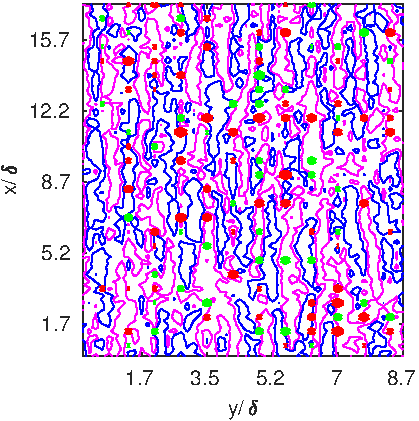
\includegraphics[width=2in,height=2in]{ek10_pi_2d_n_9_m_9_lvl_33-eps-converted-to}}}{}% 
%		  \put(0,150){(a)}
%		\end{picture}
%	\end{minipage}%
%	\begin{minipage}{0.333\textwidth}
%	    \begin{picture}(100,150)
%		    \put(0,0){{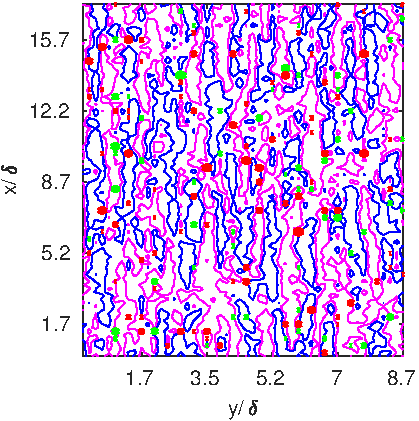
\includegraphics[width=2in,height=2in]{ek10_pi_2d_n_9_m_8_lvl_33-eps-converted-to}}}{}% 
%		    \put(0,150){(b)}
%		  \end{picture}
%	\end{minipage}%	
%	\begin{minipage}{0.334\textwidth}
%	  \begin{picture}(100,150)
%		  \put(0,0){{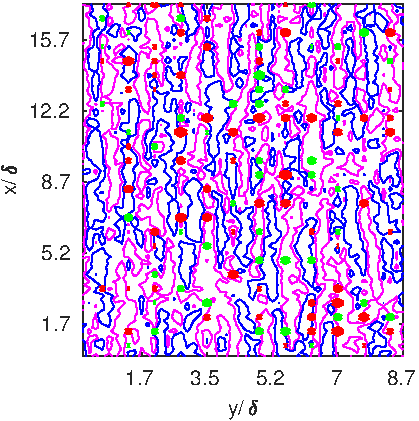
\includegraphics[width=2in,height=2in]{ek10_pi_2d_n_9_m_7_lvl_33-eps-converted-to}}}{}% 
%		  \put(0,150){(c)}
%		\end{picture}
%  \end{minipage}	
%  
%	\begin{minipage}{0.333\textwidth}
%	  \begin{picture}(100,150)
%		  \put(0,0){{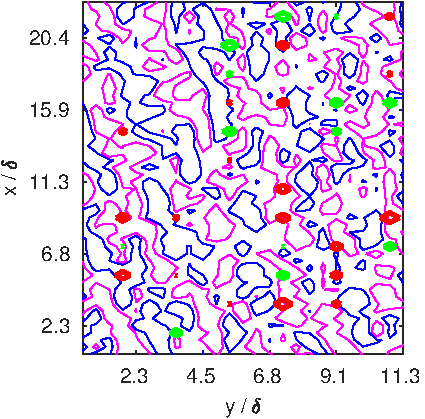
\includegraphics[width=2in,height=2in]{ek02_pi_2d_n_9_m_9_lvl_25-eps-converted-to}}}{}% 
%		  \put(0,150){(d)}
%		\end{picture}
%	\end{minipage}%
%	\begin{minipage}{0.333\textwidth}
%	    \begin{picture}(100,150)
%		    \put(0,0){{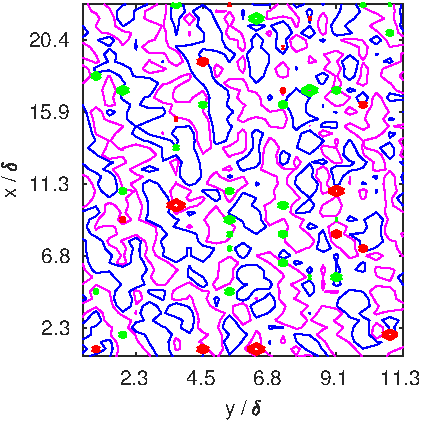
\includegraphics[width=2in,height=2in]{ek02_pi_2d_n_9_m_8_lvl_25-eps-converted-to}}}{}% 
%		    \put(0,150){(e)}
%		  \end{picture}
%	\end{minipage}%	
%	\begin{minipage}{0.334\textwidth}
%	  \begin{picture}(100,150)
%		  \put(0,0){{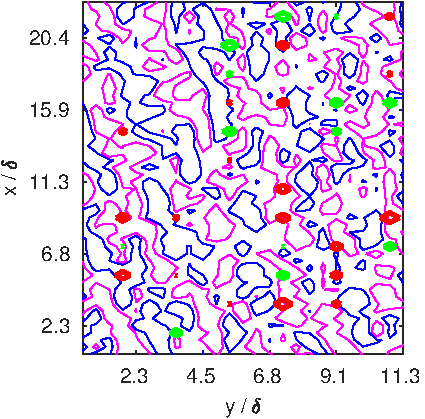
\includegraphics[width=2in,height=2in]{ek02_pi_2d_n_9_m_7_lvl_25-eps-converted-to}}}{}% 
%		  \put(0,150){(f)}
%		\end{picture}
%  \end{minipage}	  
%}
%\caption{Contour of extreme events of energy transfer between scales overlaid on u-velocity contour plots, $EK10$ case (a, b, c) and $EK02$ case (d, e, f). High velocity contours are plotted in Blue with a value of $\left < u \right >+0.5 \sigma_u$, low velocity contours are plotted in Purple with a value of $\left < u \right >-0.5 \sigma_u$. Green and Red contours are plotted for extreme events of inter-scale energy transfer between two scales for values of $-3\sigma_{t^{(m,n)}}$ and $3\sigma_{t^{(m,n)}}$, respectively. (a), (b), (c) represents energy transfer from scale $0.178\delta$, $0.348\delta$, $0.697\delta$ to a scale of spatial extent $0.178\delta$ for $EK10$ at a height of $0.515\delta$. (d), (e), (f) represents energy transfer from scale $0.454\delta$, $0.908\delta$, $1.815\delta$ to scale $0.454\delta$ for $EK02$ on a wall-parallel plane at a height of $0.49\delta$, respectively.} 
%\label{fig:inter_scale_energy_2d}
%\end{figure}

\section{Summary and Conclusions}
The existence of VLSMs as slender and elongated low- or high-momentum regions clearly marked with borders has been confirmed from visual inspection of the flow fields in the atmospheric boundary layer \citep{traumner_blm_2015}. The importance of these structures is of interest because of the fact that any turbulent flow exhibits a hierarchy of motions of different scales. The role of VLSMs in this hierarchy is not completely defined. One important aspect of VLSMs is that they influence or modulate small-scale motions and the characterization of this modulation was explored in Sec. \ref{Modulation_VLSMs}. For this analysis on modulation effect, the large scale has been defined as any motion with a scale larger than $2\delta$. The same analysis was carried out with a cut-off scale of $5\delta$ to separate large and small scales. Irrespective of the definition of large scales, qualitatively, results did not change. It was observed that large-scale fluctuations correlate with small-scale fluctuations in agreement with previous work \citep{ganapathi_jfm_2012_modulation} and that the degree of fluctuation in large scales dictates the degree of fluctuation in small scales with large fluctuations in large scales corresponding to large fluctuations in small scales. The frequency of fluctuations of small scales, however, is not strongly correlated to the strength of fluctuations of large scale in the log and outer region and appears to be a function of height. The magnitude of Reynold's stress is inversely correlated to the intensity of large-scale fluctuations. This observation bears importance in automated detection algorithms of VLSMs in any flow field and suggests that VLSMs are most likely to be found as areas characterized by lower Reynold's stresses.  

The mechanism of exerting influence on small-scale dynamics by large scales is explored through interscale energy exchange in the wavelet domain. The main question was whether nonlocal energy transfer would be responsible for the influence of VLSMs on small-scale motions. It was observed that the magnitude of nonlocal energy transfer in the three examined cases was insignificant compared to the local energy transfer. There was no evidence found that VLSM or LSM could significantly impact small-scale turbulent motions through nonlocal energy transfer. Another question was whether weak rotation would impact energy transfer between scales and ultimately impact the organization of VLSMs and LSMS. This was particularly important due to the fact that in the environment at large scales, Coriolis force cannot be ignored. Prior work has shown that for very low Rossby number including the limiting case of solid body rotation (zero $Ro$ number), the energy transfer characteristics change even though the Coriolis force is absent from the $tke$ transport equation \citep{yeung_zhou_pof_98, hossain_pof_94}. Weak rotation as has been interrogated in this study also shows its impact on the energy distribution over length scales. This is evident from the one-dimensional spectra of the streamwise velocity (Fig. \ref{fig:spectra_fw}). Unlike pressure-driven channel flow, a very narrow band of scales contain most of the $tke$ when there is a Coriolis force. This could indicate the inhibition of the development of VLSMs or shortening of the length scale of VLSMs. However, significant changes in the local, nonlocal energy transfer characteristics were not observed, an indication that the fundamental turbulent dynamics were not altered although the ratio of the largest to smallest energy containing length scales did change when Coriolis force was introduced.

As the method responsible for the organisation of VLSMs, GH12 associated the well-known paradigm of the train of hairpin vortices where counter rotating vortices align themselves along the streamwise direction spaced by the inclined, induced long regions of low- and high-speed fluids. From kinematic consideration, this scenario stands out as a possible organization of the constituent coherent structures that shape VLSMs. By coherent structures, we refer to a conglomeration of phase-correlated vortices following the definition adopted by Hussain  \citep{hussain_1983_csreality} and prefer to maintain a clear distinction between coherent structures and VLSMs,  which are often mixed up and used interchangeably in the literature. This distinction is important to maintain to understand the physical energy cascade process. Although scale-scale interaction or the turbulent energy content over scales is analysed in spectral space or wavelet space, the physical mechanism of transfer is most often explained by vorticity dynamics. There is an apparent disconnect between energy density over assumed wavelike motions, which do not really exist in a turbulent flow field, and the physical mechanism of vortex stretching or merging through which energy transfers to smaller scales or travels towards larger scales, respectively. 

The physical mechanism of energy transfer from large to smaller scales corresponds to breaking up of large energy containing coherent motions \citep[chap. 5]{davidson_turb_book}. Irrespective of the background mechanism responsible for the formation of LSMs and VLMSs, the interscale energy transfer characteristics as explored here indicate that it is possible for smaller scale motions to merge together to form large-scale motions. This prediction can be attributed to the observed transfer of energy from small to large scales. However, a hierarchy of this merging process is also observed. In general, smaller scale motions combine to form a larger scale motions and those larger scale motions would combine to form even larger scale motions. However, the reverse cascading of energy does not break the observance of Richardson's prescribed forward energy cascading. The energy transfer from large to small scales always dwarfs the energy transfer from small to large scales. The observed energy exchange process and spectra here lend support toward the hypothesis that LSMs concatenate to form VLSMs as suggested by \citet{kim_adrian_pof99, balakumar_adrian_ptrs_07, baltzer_jfm_13}.

\bibliographystyle{unsrtnat}
\bibliography{MyThesisRefs}
\clearpage
%% ======================= ALL TABLES ====================

\begin{table}
\centering
\footnotesize
\caption{Simulation parameters}
\centering
\begin{tabular}{ c c c c c c c c c c c c}
\hline 
 & Nx & Ny & Nz & $L_x$(Km) & $L_y$(Km) & $L_z$ (Km) & $U_g$ (m/s) & $u_*$ (m/s) & $\delta$(m) & $Ro$ & $f(s^{-1})$ \\
\hline 
$EK10$ & 2048 & 2048 & 64 & 120 & 120 & 1.5 & 10  & 0.41 & 1433.00  & 67 & 10$^{-4}$  \\
$EK02$ & 2048 & 2048 & 64 & 120 & 120 & 0.75 & 2 & 0.09 & 550.69 & 33 & 10$^{-4}$ \\
$CHNL$ & 2048 & 2048 & 64 & 120 & 120 & 1.5 & 0 & 0.42  & 1500.00 & - & - \\
\hline 
\hline 
\end{tabular}
\label{tab:sim_param}
\end{table}

\begin{table}
	  \caption{Wavelet decomposition levels and corresponding normalised horizontal length scales ($r_m/\delta$) and wavenumbers ($k_m\delta$) of all three cases.}	
	    \centering
		\begin{tabular}{cllllllll}
		\hline \hline\\
		Wavelet Decomposition Level (m/n) &  \multicolumn{2}{c}{CHNL} &  & \multicolumn{2}{c}{EK10} & & \multicolumn{2}{c}{EK02}\\
		\hline \\
		{}   & {$r_{m}/\delta$}   & {$k_m\delta$}  &   & {$r_{m}/\delta$}    & {$k_{m}\delta$} &  & {$r_{m}/\delta$}   & {$k_{m}\delta$} \\
		1  & 42.666 & 0.147   &   &  44.66    & 0.140  &  & 116.21    & 0.0541 \\ 
		2  & 21.333 & 0.294   &   &  22.33    & 0.281  &  & 58.109    & 0.1081 \\
		3  & 10.666 & 0.589   &   &  11.16    & 0.562  &  & 29.054    & 0.2163 \\
		4  & 5.333  & 1.178   &   &  5.582    & 1.125  &  & 14.527    & 0.4325 \\
		5  & 2.666  & 2.356   &   &  2.791    & 2.250  &  & 7.2637    & 0.8650 \\
		6  & 1.333  & 4.712   &   &  1.395    & 4.501  &  & 3.6319    & 1.7300 \\
		7  & 0.666  & 9.424   &   &  0.697    & 9.003  &  & 1.8159    & 3.4600 \\
		8  & 0.33   & 18.849  &   &  0.348    & 18.00  &  & 0.9080    & 6.9201 \\
		9  & 0.166  & 37.699  &   &  0.174    & 36.01  &  & 0.4540    & 13.840 \\
		10 & 0.083  & 75.398  &   &  0.087    & 72.02  &  & 0.2270    & 27.680 \\
		\hline\hline
		\end{tabular}	
	
	\label{tab:wav-mode2scale}
\end{table}
% ================ ALL FIGURES =============================
% ------------------- modulation ------------------------
\graphicspath{{chap2Img/}}
\begin{figure}[htb]
\centering {
	\begin{minipage}{0.99\textwidth}
	\setlength{\unitlength}{1in}
	  \begin{picture}(6.5,5.5)
		  \put(0,0){{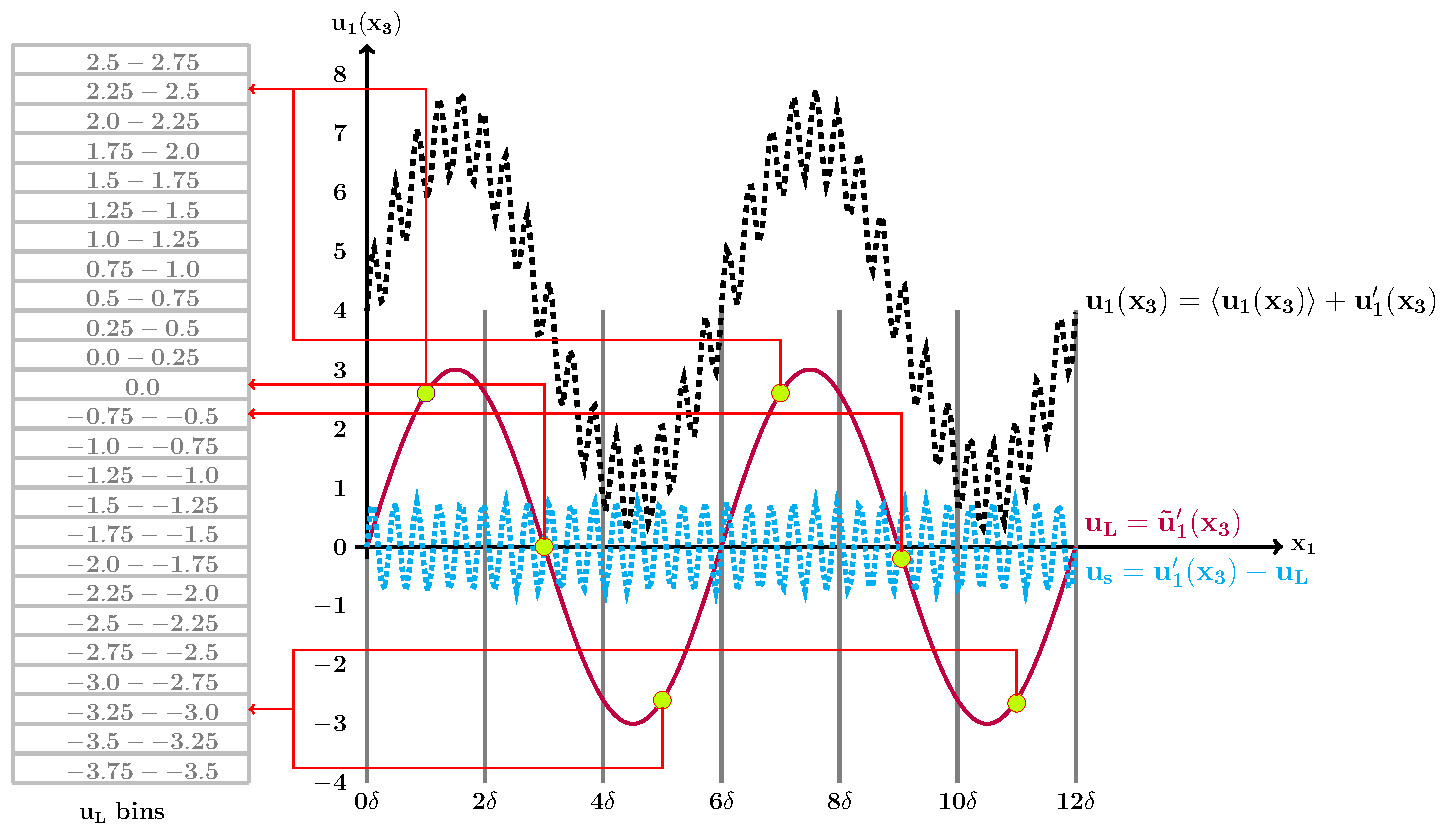
\includegraphics[width=6.0in,height=5.5in]{modulation_diagram}}}{}% 
		\end{picture}
	\end{minipage}%
	}
\caption{An illustration of the data extraction method used to investigate the modulation of the small-scale motions by large-scale motions is shown. The black dashed line in the figure represents a raw velocity signal ($u_1(x_3)$) extracted along a line in $x_1$-direction from the simulated flow field. The filtered large-scale fluctuation ($u_L$) is represented by the red smooth line. The dotted blue line represents the data series of small-scale fluctuation ($u_s$). On the left, a hypothetical binning process for the $u_L$ series is shown and  the association of the representative $u_L$ values to the correct bin is shown with arrows.}
\label{fig:modulation}
\end{figure}

% ============== variation of us2 as a function of z for different uL ======================
\graphicspath{{chap2Img/}}
\begin{figure}[htb]
\centering {
	\begin{minipage}{0.333\textwidth}
	  \begin{picture}(100,150)
		  \put(-5,0){{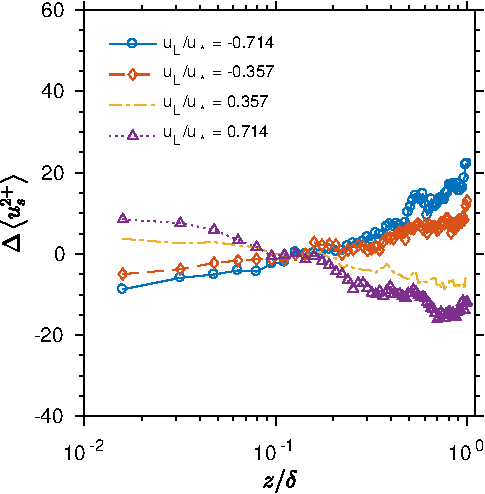
\includegraphics[width=2in,height=2in]{chnl_u_s2_z_multiple_u_l_0-eps-converted-to}}}{}% 
		  \put(40,30){(a)}
		\end{picture}
	\end{minipage}%
	\begin{minipage}{0.3333\textwidth}
	    \begin{picture}(100,150)
		    \put(0,0){{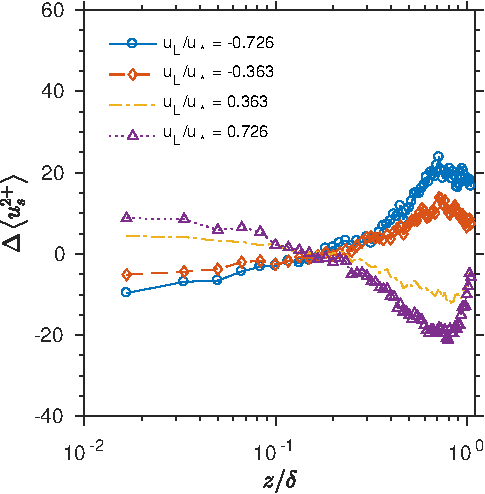
\includegraphics[width=2in,height=2in]{ek10_u_s2_z_multiple_u_l_0-eps-converted-to}}}{}% 
		    \put(40,30){(b)}
		  \end{picture}
	\end{minipage}%	
	\begin{minipage}{0.34\textwidth}
	  \begin{picture}(100,150)
		  \put(0,0){{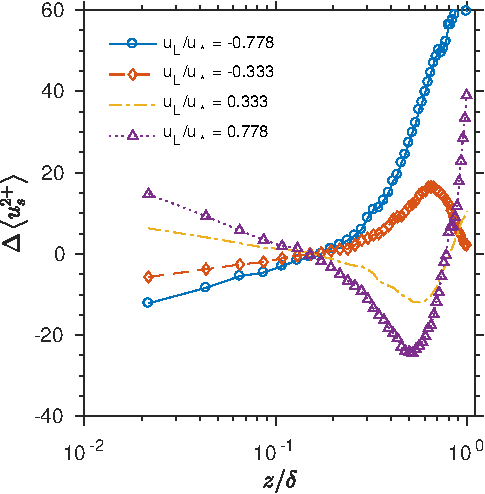
\includegraphics[width=2in,height=2in]{ek02_u_s2_z_multiple_u_l_0-eps-converted-to}}}{}% 
		  \put(40,30){(c)}
		\end{picture}
  \end{minipage}	    
}
\caption{The relative strength of small-scale fluctuations conditioned on the strength of fluctuations of large scales as defined in Eq. \ref{eq:relative_var_us2} for the three different flow cases, (a) $CHNL$, (b) $EK10$, and (c) $EK02$.}
\label{fig:us2_uL}
\end{figure}

% =============== variation of kx_us as a function of z for different uL ======================
\graphicspath{{chap2Img/}}
\begin{figure}[htb]
\centering {
	\begin{minipage}{0.333\textwidth}
	  \begin{picture}(100,150)
		  \put(0,0){{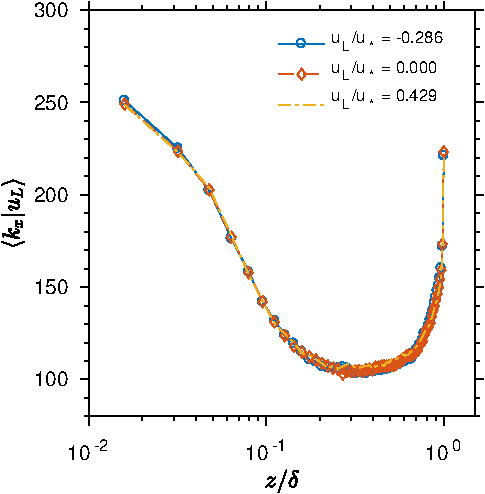
\includegraphics[width=2in,height=2in]{chnl_kx_ul_z-eps-converted-to}}}{}% 
		  \put(35,30){(a)}
		\end{picture}
	\end{minipage}%
	\begin{minipage}{0.333\textwidth}
	    \begin{picture}(100,150)
		    \put(0,0){{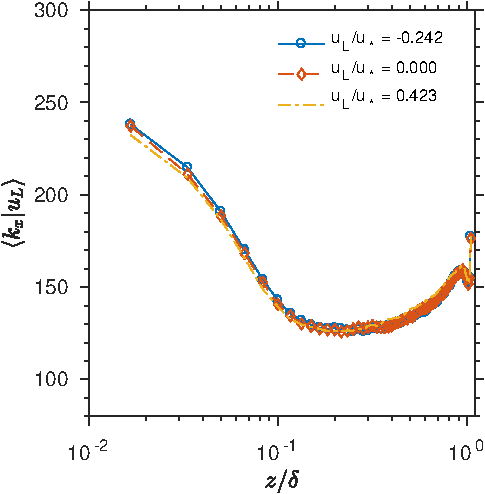
\includegraphics[width=2in,height=2in]{ek10_kx_ul_z-eps-converted-to}}}{}% 
		    \put(35,30){(b)}
		  \end{picture}
	\end{minipage}%	
	\begin{minipage}{0.334\textwidth}
	  \begin{picture}(100,150)
		  \put(0,0){{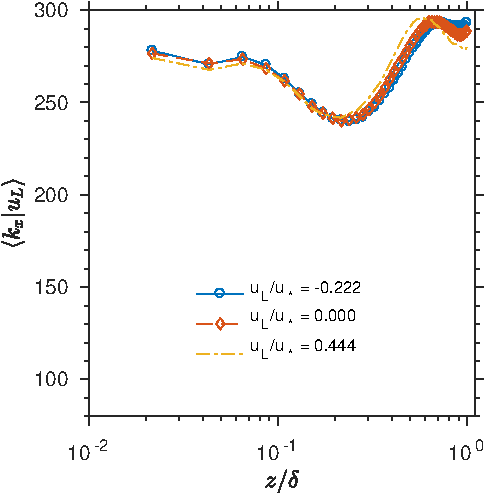
\includegraphics[width=2in,height=2in]{ek02_kx_ul_z-eps-converted-to}}}{}% 
		  \put(35,30){(c)}
		\end{picture}
  \end{minipage}	
}
\caption{The wavenumber quantifying the scale of fluctuation of primary turbulent motions as a function of large-scale fluctuation intensities for the three cases, (a) $CHNL$, (b) $EK10$, and (c) $EK02$.}
\label{fig:kx_ul}
\end{figure} 


% ===== variation of u'w' as a function of z for different uL ======================
\graphicspath{{chap2Img/}}
\begin{figure}[htb]
\centering {
	\begin{minipage}{0.333\textwidth}
	  \begin{picture}(100,150)
		  \put(0,0){{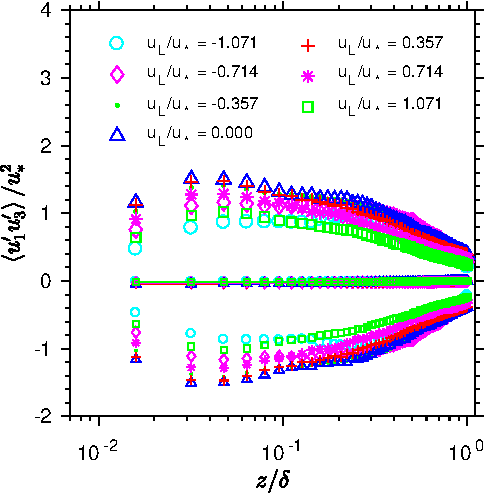
\includegraphics[width=2in,height=2in]{chnl_u_l_uw_std-eps-converted-to}}}{}% 
		  \put(28,30){(a)}
		\end{picture}
	\end{minipage}%
	\begin{minipage}{0.333\textwidth}
	    \begin{picture}(100,150)
		    \put(0,0){{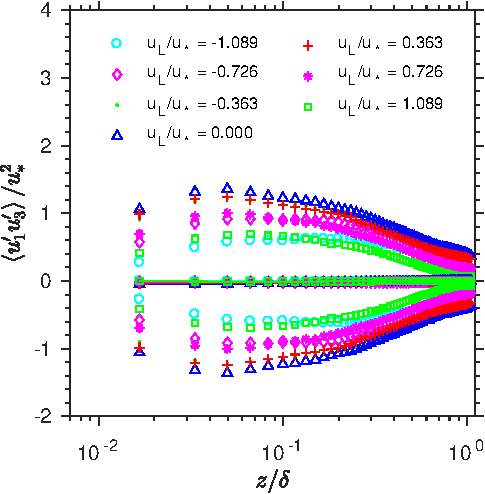
\includegraphics[width=2in,height=2in]{ek10_u_l_uw_std-eps-converted-to}}}{}% 
		    \put(28,30){(b)}
		  \end{picture}
	\end{minipage}%	
	\begin{minipage}{0.334\textwidth}
	  \begin{picture}(100,150)
		  \put(0,0){{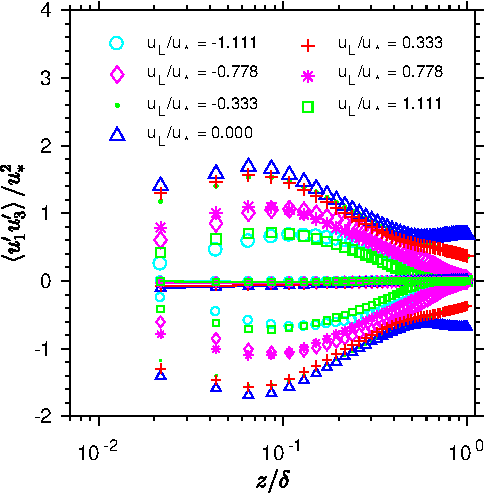
\includegraphics[width=2in,height=2in]{ek02_u_l_uw_std-eps-converted-to}}}{}% 
		  \put(28,30){(c)}
		\end{picture}
  \end{minipage}	
}
\caption{The wall-normal Reynolds shear stress, $u^\prime w^\prime$, normalized by the surface shear stress as a function of large-scale fluctuations and distance in the wall-normal direction for each of the cases, (a) $CHNL$, (b) $EK10$, and (c) $EK02$. Solid lines correspond to the mean shear stress, $\left< u^\prime w^\prime \right>_{u_L}$, and points correspond to $\pm 3 \sigma_{u_L}^{u^\prime w^\prime}$.} 
\label{fig:uw_uL}
\end{figure}

%========================== Figure: Spectra ====================================
\graphicspath{{chap2Img/}}
\begin{figure}[htb]
\centering {
	\begin{minipage}{0.33\textwidth}
	\setlength{\unitlength}{1in}
	\begin{picture}(2.1,2)
		\put(0,0){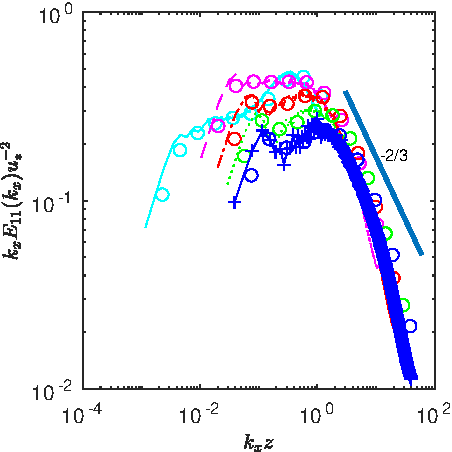
\includegraphics[width=1.9in,height=2in]{wavelet_n_fourier_spectra_chnl_pre-eps-converted-to}}{}% 
		\put(0.45,0.45){($\mathbf{a}$)}
	\end{picture}	
	\end{minipage}%
	\begin{minipage}{0.33\textwidth}
	\setlength{\unitlength}{1in}
	\begin{picture}(2.1,2)
		\put(0,0){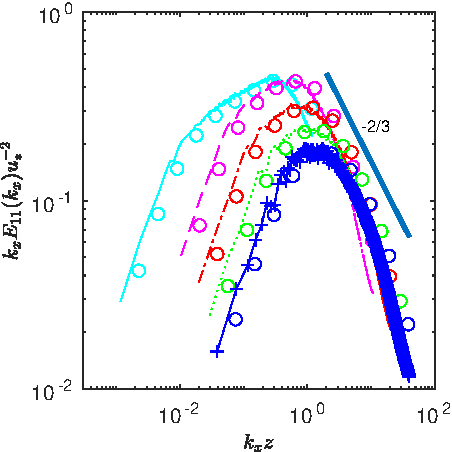
\includegraphics[width=1.9in,height=2in]{wavelet_n_fourier_spectra_ek10_pre-eps-converted-to}}{}%
		\put(0.45,0.45){($\mathbf{b}$)}
		\end{picture}
	\end{minipage}%	
		\begin{minipage}{0.33\textwidth}
		\setlength{\unitlength}{1in}
		\begin{picture}(2.1,2)
	  \put(0,0){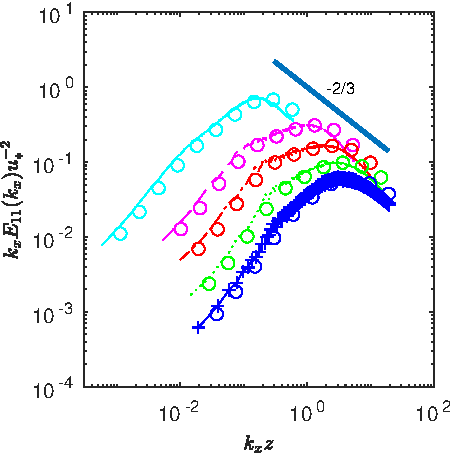
\includegraphics[width=1.9in,height=2in]{wavelet_n_fourier_spectra_ek02_pre-eps-converted-to}}{}%
	  \put(0.45,0.45){($\mathbf{c}$)}
	  \end{picture}
\end{minipage}	
}
\caption{Premultiplied wavelet and Fourier spectra of streamwise velocity component, averaged over spanwise direction for (a) $CHNL$, (b) $EK10$, and (c) $EK02$ at different wall-normal locations. Spectra are plotted against wavenumbers normalized by height. Lines represent Fourier spectra and circles represent wavelet spectra. Line types {\tiny ---,$--$, $- \cdot$, $\cdot \cdot \cdot$, $-+$}  correspond to heights ($0.01\delta$, $0.14\delta$, $0.26\delta$, $0.39\delta$, $0.52\delta$) for $CHNL$, ($0.01\delta$, $0.14\delta$, $0.28\delta$,$0.41\delta$, $0.54\delta$) for $EK10$, and ($0.04\delta$, $0.19\delta$, $0.34\delta$, $0.54\delta$, $0.71\delta$) for $EK02$.}
\label{fig:spectra_fw}
\end{figure}

\graphicspath{{chap2Img/}}
\begin{figure}[htb]
	\begin{minipage}{\textwidth}
	\setlength{\unitlength}{1in}
	  \begin{picture}(6,4)
		\put(0.5,0){\includegraphics[width=5.0in,height=3.9in]{tmn_chnl_fixed_n-eps-converted-to}}
	%	\put(-0.1,2.5){$\mathbf{(a)}$}
	  \end{picture}
	\end{minipage}
\caption{Wavelet dual bi-spectrum of subgrid scale transfer normalized by $u_*^3$ for the $CHNL$ case. This figure shows the rate of energy transfer over unit area per unit length of scale where energy transfer occurs from scales $r_{m}/\delta$ to scales smaller than $r_{n}/\delta$.}	
\label{fig:tmn_fixed_n_chnl}
\end{figure}%
\begin{figure}
	\begin{minipage}{\textwidth}
	\setlength{\unitlength}{1in}
	\begin{picture}(6,4)
		\put(0.5,0){\includegraphics[width=5.0in,height=3.9in]{tmn_ek10_fixed_n-eps-converted-to}}
		%\put(-0.1,2.5){$\mathbf{(b)}$}
	\end{picture}
	\end{minipage}
\caption{The rate of energy transfer over unit area per unit length of scale is shown for the $EK10$ case where energy transfer occurs from scales $r_{m}/\delta$ to scales smaller than $r_{n}/\delta$. Energy transfer is normalized by $u_*^3$. }	
\label{fig:tmn_fixed_n_ek10}
\end{figure}

\begin{figure}	
	\begin{minipage}{\textwidth}
	\setlength{\unitlength}{1in}
	\begin{picture}(6,4)
	\put(0.5,0){\includegraphics[width=5.0in,height=3.9in]{tmn_ek02_fixed_n-eps-converted-to}}
	%\put(-0.1,2.5){$\mathbf{(c)}$}
	\end{picture}
\end{minipage}	
\caption{Wavelet dual bi-spectrum of subgrid scale transfer normalised by $u_*^3$ for $EK02$. Energy transfer is measured over unit area per unit length of scale and transfer occurs from scales $r_{m}/\delta$ to scales smaller than $r_{n}/\delta$.}
\label{fig:tmn_fixed_n_ek02}
\end{figure}%


\graphicspath{{chap2Img/}}
\begin{figure}
	\begin{minipage}{\textwidth}
	\setlength{\unitlength}{1in}
	  \begin{picture}(6,4)
		\put(0.5,0){\includegraphics[width=5.0in,height=3.9in]{tmn_chnl_fixed_n-m_n_equal-eps-converted-to}}
		%\put(-0.1,2.5){$\mathbf{(a)}$}
	  \end{picture}
	\end{minipage}
\caption{Wavelet dual bi-spectrum of subgrid scale transfer normalised by $u_*^3$ for the $CHNL$ case. In contrast to Fig. \ref{fig:tmn_fixed_n_chnl}, this figure shows the transfer occurring between length scales $r_m$ to $r_m$ ($r_n \equiv r_m$)}	
\label{fig:tmn_fixed_n_meqn_chnl}
\end{figure}

\begin{figure}
	\begin{minipage}{\textwidth}
	\setlength{\unitlength}{1in}
	\begin{picture}(6,4)
		\put(0.5,0){\includegraphics[width=5.0in,height=3.9in]{tmn_ek10_fixed_n-m_n_equal-eps-converted-to}}
		%\put(-0.1,2.5){$\mathbf{(b)}$}
	\end{picture}
	\end{minipage}
\caption{Wavelet dual bi-spectrum of subgrid scale transfer normalised by $u_*^3$ for the $EK10$ case. In contrast to Fig. \ref{fig:tmn_fixed_n_ek10}, this figure shows the transfer occurring between length scales $r_m$ to $r_m$ ($r_n \equiv r_m$)}	
\label{fig:tmn_fixed_n_meqn_ek10}
\end{figure}
	
\begin{figure}
	\begin{minipage}{\textwidth}
	\setlength{\unitlength}{1in}
	\begin{picture}(6,4)
	\put(0.5,0){\includegraphics[width=5.0in,height=3.9in]{tmn_ek02_fixed_n-m_n_equal-eps-converted-to}}
	%\put(-0.1,2.5){$\mathbf{(c)}$}
	\end{picture}
\end{minipage}	
\caption{Wavelet dual bi-spectrum of subgrid scale transfer normalised by $u_*^3$ for the $EK02$ case. The energy transfer from scale $r_m$ to $r_n (\equiv r_m)$ is shown in contrast to Fig. \ref{fig:tmn_fixed_n_ek02} where, $r_n < \frac{1}{2}r_m$.}
\label{fig:tmn_fixed_n_meqn_ek02}
\end{figure}%

\graphicspath{{chap2Img/}}
\begin{figure}
\centering {
	\begin{minipage}{0.5\textwidth}
	  \begin{picture}(100,180)
		  \put(0,-5){{\includegraphics[width=2.85in,height=2.37in]{pi_chnl_diff_n_by_u3_dz_2-eps-converted-to}}}
		  \put(0,150){($a$)}
		\end{picture}
	\end{minipage}%
	\begin{minipage}{0.49\textwidth}
	    \begin{picture}(100,180)
		    \put(0,-5){{\includegraphics[width=2.85in,height=2.37in]{pi_chnl_diff_n_by_u3_dz-eps-converted-to}}}
		    \put(0,150){($a^\prime$)}
		  \end{picture}
	\end{minipage}%
		
	\begin{minipage}{0.5\textwidth}
	  \begin{picture}(100,180)
		  \put(0,-5){{\includegraphics[width=2.85in,height=2.37in]{pi_ek10_diff_n_by_u3_dz_2-eps-converted-to}}} 
		  \put(0,150){($b$)}
		\end{picture}
  \end{minipage}	
	\begin{minipage}{0.49\textwidth}
  \begin{picture}(100,180)
	  \put(0,-5){{\includegraphics[width=2.85in,height=2.37in]{pi_ek10_diff_n_by_u3_dz-eps-converted-to}}}
	  \put(0,150){($b^\prime$)}
	\end{picture}
  \end{minipage}

	\begin{minipage}{0.5\textwidth}
	  \begin{picture}(100,180)
		  \put(0,-5){{\includegraphics[width=2.85in,height=2.37in]{pi_ek02_diff_n_by_u3_dz_2-eps-converted-to}}} 
		  \put(0,150){($c$)}
		\end{picture}
  \end{minipage}	
	\begin{minipage}{0.49\textwidth}
  \begin{picture}(100,180)
	  \put(0,-4){{\includegraphics[width=2.85in,height=2.37in]{pi_ek02_diff_n_by_u3_dz-eps-converted-to}}} 
	  \put(0,150){($c^\prime$)}
	\end{picture}
\end{minipage}
}
\caption{Aggregate subgrid scale energy transfer from large to small scales separated by an arbitrary cut-off scale. For panels on the left, total subgrid transfer is calculated using Eqn. \ref{pi_tmn_1} and the right-hand side panels correspond to total subgrid transfer calculated following the definition in Eqn. \ref{pi_tmn}. }
\label{fig:pi_tmn}
\end{figure}
%=========================================================

%%% -*-LaTeX-*-
\chapter{Time scale of very large scale motions}\label{chap:chap3}
Dynamic Mode Decomposition (DMD) has been used to study the time scale of Very Large Scale Motions (VLSMs) in the atmospheric boundary layers. While the length scales of VLSMs have been identified in previous studies, the time scale of evolution has not been identified objectively. It was reported in the earlier studies that VLSMs convect with a velocity lower than the local mean velocity. The time scales of VLSMs were found to be much larger than the large eddy turnover time, which is in line with the previous findings. DMD results also show that low-momentum and high-momentum regions appear alternatively in the spanwise direction as was observed from experiments and other visualization methods. However, the spanwise extent of the VLSMs appears to be significantly lower than what was estimated by earlier studies.


\section{Introduction}
Understanding the hierarchy of scales and how these scales interact is fundamental towards understanding  turbulent flow phenomena and devising mechanisms to control turbulent mixing processes. A common line of inquiry is to examine the spatial organization of turbulent motions at different scales using flow visualization technique. Typically, a visualization experiment is carried out using a passive scalar as a tracer. Such experiments can reveal the presence of multiple hierarchical scales and their relative motions. For example, a silhouette image of a large-scale structure resulting from the conglomeration of finer scale motions has been captured in  Boundary Layer (BL) flows \citep{falco_pof_77, hommema_adrian_blm_03}. These visualization experiments by \citet{falco_pof_77} and \citet{hommema_adrian_blm_03} provided insight on the organization of large-scale motions in the BL including the visual identification of inclined ramp like structures previously identified. However, \citet{hussain_1986_jfm} discussed caveats of visualisation technique and emphasizes that caution must be taken in interpretation of scalar marked boundary lines of structures. Still, when a sufficient description of the flow field is available from a simulation or experiment, data driven modeling can be used as a surrogate of the experimental methods while avoiding some of the limitations of experimental methods. One of the convincing qualities of data-driven methods is that they  do not heavily depend on the use of subjective parameters as used in conventional conditional averaging. Among the data-driven techniques, mainly two methods, i.e., Proper Orthogonal Decomposition (POD) \citep[eg., ][]{li_bouzeid_blm_2011,muld_compFluids_2012} and Dynamic Mode Decomposition (DMD). \citep[eg., ][]{bagheri_jfm2013,liu_ExpF_2015,muld_compFluids_2012} have been used widely. \citet{taira_arxiv_2017} summarized the most important strengths and weaknesses of both methods. 

A general strategy of studying flow structures is to project velocity fields on to different basis vectors i.e., Fourier modes, empirical eigen vectors, and discrete wavelet basis vectors. The velocity field is usually decomposed as a linear combination of orthogonal basis functions at a given time as $u(\mathbf{x},t) = \sum_k a_k \phi_k(\mathbf{x},t)$ where $\phi_k(\mathbf{x})$ represents the basis vectors and $a_k$ represents coefficients of the projections. Alternatively, it is possible to decompose the velocity field into a fixed set of orthogonal spatial functions with time-dependent projection coefficients,  i.e., $u(\mathbf{x},t)=\sum_k a_k(t) \phi_k(\mathbf{x})$  where $u(\mathbf{x},t)$ denotes a velocity field, $a_k(t)$ denotes the time-dependent  coefficients of projection, and $\phi_k(\mathbf{x})$ denotes orthogonal spatial functions capturing the spatial description of the field \citep{taira_arxiv_2017}. Such a decomposition underpins the Galerkin projection schemes used in computational fluid dynamics \citep{rowley2004model, armbruster_chaos_94} and form the basis of  the Proper orthogonal Decomposition (POD), which is a common tool to identify the spatial structures of energetic scales in a turbulent flow and has been used to study the spatial structure of Very Large Scale Motions (VLSMs) \citep[][]{Hellstrom_pof_2011,bailey_smits_jfm_2010}. However, to study the temporal evolution of motions at any scale, a POD based gelarkin projection scheme must be adopted to determine the time dependent expansion coefficients. A POD basis is extracted from a full-scale simulation and then the system is modeled on a reduced set of the POD bases. Next, proper boundary and initial conditions for the new basis are set before solving the resultant system of ordinary differential equations in order to determine the time-dependent expansion coefficients ($a_k(t)$) \citep[eg,. ][]{stabile2017advances}. If only the spatial structure coherent motions is of interest, determining the spatial basis vectors $\phi_k(\mathbf{x})$ is sufficient. Many studies have used POD to this end \citep[eg., ][]{li_bouzeid_blm_2011,muld_compFluids_2012}. 

The relatively new method of modal decomposition, namely Dynamic Mode Decomposition (DMD), is advantageous in short time flow evolution studies. DMD is completely data driven and does not require any knowledge of the underlying conservation laws that govern the dynamics, unlike POD method. Another attractive feature of DMD is that it can isolate dynamic structures with a particular frequencies where POD modes can correspond to a mix of frequencies. This feature makes DMD useful to isolate and rank structures that evolve at different time scales and study their spatial patterns. DMD have been successfully used to identify structures behind bluff bodies, but has so far not been used to characterize VLSMs in the high Reynold's number boundary layer where the only restriction on scale separation is the dynamic range of the simulation and experimental data in contrast to finite Reynold's number direct numerical simulation studies.  In this study, DMD is used to study the spatial and temporal characteristics of VLSMs in the atmospheric boundary layers under two different forcing conditions. 

\section{Large Eddy Simulation}
Large Eddy Simulation (LES) was carried out to simulate an Ekman layer and flow in a channel. Resolution in horizontal and vertical directions were $62.5\ m$ and $7.89\ m$, respectively. The same numerical LES code along with the same subgrid-scale model that was used to study VLSM characteristics in Chapters \ref{chap:chap1} and \ref{chap:chap2} has been used to generate the flow fields (see Sec. \ref{sec:num_sim_chap_1} and \ref{sec:LES_chap2} ). However, to keep the computational cost of the DMD analysis within a reasonable limit, grid points in horizontal directions were reduced to 768 and in the vertical direction, a total of 96 grid points. The flow domain spanned $48$ Km in the horizontal ($x$, $y$) directions and 750.0 m in the wall-normal direction ($z$) for $EK02$ and 1500.0 m for $CHNL$. The parameters of the simulations are shown in Table \ref{tab:sim_param}. The reduced domain size here should not pose any limitations to the evolution of VLSMs because the results in Chapter \ref{chap:chap1} confirms that the maximum length scale of VLSMs is no larger than $25\delta$.

%An analysis of 8000 instantaneous two dimensional frames of u-velocity component required analysing a data matrix of 37.74 gigabyte. %A decomposition of the full three dimensional u-component of the velocity field into DMD modes would require operations to be carried over a data matrix of size 3.62 terabyte. 


\section{Dynamic Mode Decomposition} DMD can be applied to experimental and numerical data sets alike. This analysis provides dynamic modes that evolve with certain frequencies and are associated with a decay or growth rate. The dynamic modes are composed of recognizable spatial patterns that can be interpreted as organizational units of fluid flow fields or loosely as eddies. The DMD method approximates the state of a system, e.g., as a component of the velocity field, $u \in R^{N}$ from one time instance ($m$) to another ($m+1$) with the Koopman operator $A$ as
\begin{align}
u_{m+1}= A u_{m}\ .
\label{eqn:iterative_reln}
\end{align}
An ensemble of $M$ snapshots of $u$ obtained with a fixed time interval $\Delta t$ between snapshots can be organized in two matrices $X$ and $Y$
\begin{align}
X & = [u_{1}\ u_{2} \ \cdots \ u_{M-1}], \\
Y & = [u_{2}\ u_{3} \ \cdots \ u_{M}]\ ,
\end{align}
which using Eqn. \ref{eqn:iterative_reln} can be rewritten as
\begin{align}
X & = [u_{1}\ Au_{1} \ \cdots \ A^{M-2}u_{1}] \label{eqn:X_approx}, \\
Y & = [Au_{1}\ A^{2}u_{1} \ \cdots \ A^{M-1}u_{1}] \label{eqn:Y_approx}. 
\end{align}
The columns of $X$ and $Y$ are each elements of a Krylov subspace and the last vector in $Y$ can be approximated within the span of the Krylov subspace in an $L^{2}$ sense \citep{kutz_book2013} as
\begin{align}
u_{M} = \sum_{i=1}^{M-1}b_{i} u_{i}+ r,
\label{eqn:last_vec_approx}
\end{align}
where $b_i$ are the coefficients of the Krylov space vectors and $r$ is the residual. Schmid \citep{schmid_jfm2010} suggests that after a critical number of snapshots, adding more snapshots in $X$ or $Y$, i.e., any more columns, would not improve the vector space spanned by $X$ and at this point, the last data vector approximation (Eqn. \ref{eqn:last_vec_approx}) would not improve any more. This could practically serve as a limit to the number of snapshots used in calculation. Up until this point, the Koopman operator $A$ is unknown. The key idea of DMD is to find an approximation to the eigen vectors and eigen values of $A$. From \ref{eqn:X_approx} and \ref{eqn:Y_approx}, a transformation relationship between $X$ and $Y$ can be expressed as
\begin{align}
 Y = A X.
\label{eqn: y=ax}
\end{align}
This matrix equation can also be rewritten following Eqn. \ref{eqn:last_vec_approx} as
\begin{align}
  Y =X S + r e^{T}_{M-1},
\end{align}
where $e_{M-1} \in R^{(M-1) \times 1}$ is the $(M-1)$th unit vector, $r \in R^{N \times 1}$, and $S \in R^{N \times (M-1)}$ is a matrix of the companion type and assumes the form
\begin{align}
S =
    \begin{bmatrix}
        0 & \cdots &        & 0  & b_1\\
        1 & \ddots &        & 0  & b_2 \\
        0 & \ddots & \ddots &    & \vdots \\
          & \ddots & \ddots & 0  & b_{M-2} \\
        0 & \cdots & 0      & 1  & b_{M-1}
    \end{bmatrix}\ .
\end{align}
The last column of $S$ contains the unknown coefficients of Eqn. \ref{eqn:last_vec_approx}. Eigen values of $S$ approximate some of the eigen values of $A$. However, calculating matrix $S$ requires the operator $A$ to be known to proceed with an Arnoldi algorithm. \citet{schmid_jfm2010} suggested calculating a matrix $\tilde{S}$ instead of $S$, where $\tilde{S}$ is a similar matrix to $A$. Utilizing reduced singular value decomposition of the data matrix $X$ and following Eqn. \ref{eqn: y=ax}, $\tilde{S}$ can be calculated from
\begin{align}
U^{*} A U  = U^{*} YW  \Sigma^{-1} \equiv \tilde{S},
\end{align}
where $X=U\Sigma W^{*}$. At this point, the following eigen value problem is solved,
\begin{align}
\tilde{S}y_{k}  =  \mu_{k} y_{k} 
\end{align}
where the eigen values $\mu_{k}$ capture the time dynamics of the discrete Koopman operator $A$ \citep{kutz_book2013}. DMD modes $\phi_{k}$ are obtained when the eigen vectors $y_{k}$ are projected to the reduced column space of $X$ as
\begin{align}
\phi_{k} = Uy_{k}.
\end{align}
The future state of the flow field at any time $n \Delta t$ can be predicted from DMD modes, 
\begin{align}
x_{n} = \sum_{k=1}^{K} b_{k} \phi_{k}(x) \text{exp}(\omega_{k} t),
\end{align}
or in matrix form, 
\begin{align}
x_{DMD}(t)= \Phi\  \text{diag}(\text{exp}(\omega t)) b,
\end{align}
where $\omega_k = \ln (\mu_{k})/ \Delta t$, $\Phi$ is a matrix whose columns are the eigen vectors $y_{k} $ and $b_{k}$ are the initial amplitudes of each mode. The $b_{k}$ amplitudes are obtained from the equation, $x_1=\Phi b$, using Moore-Penrose pseudo-inverse $\Phi^{+}$ such that,
\begin{equation}
 b = \Phi^{+}x_{1} .
\end{equation}
The algorithm as has been described was first proposed by \citet{schmid_jfm2010} and a more elaborate version can be found in \citep{kutz_book2013, rowley_mezic_schlatter_jfm_2009,tu_thesis}. This is the most widely used DMD algorithm, although a proliferation of modified DMD algorithms exists that have been observed to have a finer separation of multiscale spatio-temporal features \citep[eg., ][]{kutz_fu_brunton_siam_2016}, can handle data sampled at irregular time intervals \citep[][]{tu_thesis}, can apply DMD to spatially sub-sampled data \citep{florimond_mathelin_pof_2015}, and can manage large and streaming datasets \citep{hemati_pof_2014}.

Following the algorithm as has been described, DMD was carried out over 8000 frames for both the cases. For $CHNL$, the constant time spacing between consecutive frames ($\Delta t$) was $0.1$ sec. and for $EK02$, it was $2$ sec. Since three dimensional DMD analysis is prohibitively expensive in terms of requirement of the Random Access Memory, two-dimensional DMD was carried out on wall parallel and spanwise-vertical planes. Data were extracted at a particular streamwise-spanwise plane from the three dimensional velocity field for all the 8000 time instances and were stacked as columns in the data matrices $X$ and $Y$ to proceed with DMD mode extraction. Each of the matrices  $X$ and $Y$ required $37.7\ GB$ of memory. In case of full 3D analysis, the matrix size will rise to $3623.8\ GB$. 

\section{Results and Discussion}
DMD separates spatial structures that have different frequencies. Here, the frequency distribution of DMD modes at different heights was examined for both cases. A series of 8000 frames that were equally spaced in time scale was analyzed resulting in 8000 DMD modes that were sorted based on frequency ($\mu_k$). Modes having zero frequency were excluded from analysis because these modes would constitute the mean flow field. Time periods of 5-10 representative DMD modes are categorized against normalized height in Table \ref{tab:dmd_freq_chnl} for $CHNL$ and in Table \ref{tab:dmd_freq_ek02} for $EK02$. DMD time periods ($\Delta T$) are the inverse of the pure sine or cosine frequencies that correspond to the DMD eigen values and they are normalized with large length and velocity scales ($\Delta T / (\delta/U(\delta))$) where ($\delta/U(\delta)$) constitutes large eddy turnover time where and $U(\delta)$ is the mean velocity at the top of the boundary layer. Differences between frequencies of the first few modes resolved at different heights are observed, although for any particular mode,  discernible trends with height are not observed. Spatial structures corresponding to DMD modes are shown in Figs. \ref{fig:chnl_dmd_modes_z_4_7} and \ref{fig:ek02_dmd_modes_z_4_24}. To characterise length scales of LSMs and VLSMs comprised of low-speed fluid, velocity fields were reconstructed from the individual DMD modes at selected heights to be utilized in the structure detection procedure. To identify structures of different length scales an alternative definition adopted in Chap. \ref{chap:chap1} was used, i.e., a connected region of low-speed fluid in the binarized flow field. In case of $CHNL$, DMD modes with normalized time periods of 12.91, 6.76, 5.75, 4.74 as categorically presented against normalized height of $0.50\delta$ in Table \ref{tab:dmd_freq_chnl} were analysed.  In case of $EK02$, the DMD modes with normalized time periods of 136.5, 37.65, 21.86, 15.17 at a height of $0.48\delta$ were selected. The key observation that emerges from Fig. \ref{fig:dmd_length_scale_dist} is that contrary to primary expectation, a particular DMD mode does not isolate a single length scale. Any DMD mode is observed to comprise a distribution of length scales. So, while DMD modes can perfectly isolate dynamics based on time scale, the isolation of coherent spatial structure may not be clean. 

From the results, it is also apparent that structures that evolve over a very long time scale can be obtained in both the log and wake layers. Since a linear proportionality between the time scale and the length scale can be established following Taylor's frozen turbulence hypothesis, it can be inferred that the DMD modes with long time period would correspond to long length scales. However, an observation Fig. \ref{fig:dmd_length_scale_dist} suggests otherwise. Fig. \ref{fig:dmd_length_scale_dist}(a) shows the normalized histogram of the size distribution of the structures in the reconstructed velocity field for the $CHNL$ and Fig. \ref{fig:dmd_length_scale_dist}(b) shows the same for $EK02$. A limit in the length scale of the identified structures is observed, e.g., for $Ek02$ the maximum identified normalized length scale is $15$, whereas the normalized DMD time scale is $37.4$. 

DMD is sensitive to the sampling frequency and follows Nyquit-Shannon sampling theorem. For the $CHNL$ case, sample velocity fields were collected every 0.1 sec and for $Ek02$, the sampling rate was 2 sec. Therefore, for $CHNL$, any process that evolves with a time period of less than 0.2 sec would not be captured by the DMD decomposition and for $EK02$, that time period would be any less than 4 sec. Since this study is concerned with LSMs and VLSMs that are presumed to correspond with very long time scales, these sampling frequencies should be sufficient. The ratio between the sampling rate of $Ek02$ and $CHNL$ is 20. This difference is reflected in the obtained time periods of DMD modes. A comparison between Tables \ref{tab:dmd_freq_chnl} and \ref{tab:dmd_freq_ek02} show that the time period of the first first few modes of $EK02$ can be as large as 11 times larger than that of $CHNL$. However, in $EK02$, the DMD modes that appeared with very large time periods do not show any coherent motions that corresponds to the expected shape or length scales of VLSMs or LSMs. For example, DMD mode with characteristic normalized time scales of 136.50, 37.65, 21.86 as portrayed in Fig.  \ref{fig:ek02_dmd_modes_z_4_24} show less prominence of VLSMs as is apparent from Fig.  \ref{fig:dmd_length_scale_dist}(b), which shows the distribution of length scales. These modes that correspond to very large time periods that also do not show recognizable coherence in the plots will most likely appear as zero modes if sampling period was lower. 

An overall observation from the Tables \ref{tab:dmd_freq_chnl} and \ref{tab:dmd_freq_ek02} and plots in Fig. \ref{fig:dmd_length_scale_dist} is that VLSMs persist for a long period of time compared to their length scale. The existence of smaller scale motions are also observed in the scale distribution of slow DMD modes as shown in Fig. \ref{fig:dmd_length_scale_dist}. 

\section{Summary and Conclusions}
Large eddy simulations were carried out to study the structure of VLSMs in a pressure-driven channel flow and in an Ekman layer flow. Eight thousand successive frames were recorded from the simulation to investigate the time and length scale of VLSMs using the DMD method. DMD method produced constituent DMD modes that correspond to individual frequencies and could project the temporal evolution of the velocity field over a period of time. The spatial pattern of the individual DMD modes corresponding to a range of frequencies within the time scale of interest were investigated to understand the spatial structure of the VLSMs. It was observed that while DMD method could isolate modes evolving under different frequencies, the spatial patterns were not distinctively unique for any of the modes. Using image processing techniques and under the assumption that connected regions on a thresholded velocity field constitute coherent structures, the reconstructed velocity fields from DMD modes were analysed. It was observed that each DMD mode contained various length scales. The results showed that within the spatial structure of any DMD mode, LSMs were dominant in numbers and the existence of VLSMs with length scales greater than $10\delta$ was rare. The results also indicated that VLSMs and LSMs can evolve over a longer time scale compared to their expected advection time scale estimated from Taylor's frozen turbulent hypothesis. 

\bibliographystyle{unsrtnat}
\bibliography{MyThesisRefs}
\clearpage
 
 %% =================== all tables ========================

    \begin{table}
    \caption{Simulation parameters}
    \centering
	\begin{tabular}{ c c c c c c c c}
	\hline 
		       & $N_1/N_2$ & $N_3$   & $L_1/L_2$(Km)  & $L_3$ (Km) & $\delta$(m)   & $Ro$ \\
    \hline 
     $EK02$    & 768       &  96     & 48             &  0.75      & 563           & 33  \\
     $CHNL$    & 768       &  96     & 48             &  1.5       & 1500          & - \\
    \hline 
    \hline 
    \end{tabular}
    \label{tab:sim_param}
    \end{table}

\begin{table}
\caption{Time period of evolution of the first five DMD modes normalized by $\delta / U(z)$ for $CHNL$. Modes were calculated at different horizontal planes characterized by normalized heights presented.}
  \begin{center}
  \begin{tabular}{  c  c c c c c  } 
  \hline
  \hline
  Normalized Height & Mode 1 & Mode 2 & Mode 3 & Mode 4 & Mode 5          \\

  \multirow{1}{4em}{$0.047\delta$}  & 27.09 & 10.19 & 6.11 & 4.63 & 3.48  \\
  \hline
  \multirow{1}{4em}{$0.095\delta$}  & 14.05 & 8.78  & 5.65 & 4.07 & 3.16  \\
  \hline
  \multirow{1}{4em}{$0.2\delta$}    & 32.07 & 11.68 & 6.49 & 5.01 & 3.75  \\
  \hline
  \multirow{1}{4em}{$0.33\delta$}   & 50.59 & 12.87 & 7.22 & 4.93 & 3.94  \\
  \hline 
  \multirow{1}{4em}{$0.50\delta$}   & 12.91 & 6.76  & 5.75 & 4.74 & 3.70  \\
  \hline
  \hline
  \end{tabular}
  \end{center}
\label{tab:dmd_freq_chnl}
\end{table}

\begin{table}
\caption{Statistics of the first five DMD modes for $EK02$. DMD time periods are normalized by $\delta / U(z)$. Modes were calculated at different horizontal planes characterized by normalized heights presented.}
\begin{center}
\small
\begin{tabular}{  c c c c c c c} 
\hline
\hline  
Normalized Height  & Mode 1 & Mode 2 & Mode 3 & Mode 4 & Mode 5  \\

\multirow{1}{4em}{$0.04\delta$}  & 115.5 & 38.6 & 22.4 & 15.4 & 11.7  \\
\hline
\multirow{1}{4em}{$0.21\delta$}  & 113.4 & 34.8 & 20.4 & 14.7 & 11.4  \\ 
\hline
\multirow{1}{4em}{$0.32\delta$} & 100.2  & 35.6 & 20.8 & 14.7 & 11.4  \\ 
\hline
\multirow{1}{4em}{$0.48\delta$} & 135.7  & 37.4 & 21.7 & 15.0 & 11.6  \\ 

\end{tabular}
\begin{tabular}{  c c c c c c} 
\hline
Normalized Height  & Mode 6 & Mode 7 & Mode 8 & Mode 9 & Mode 10 \\

\multirow{1}{4em}{$0.04\delta$} & 9.6 & 8.1 & 7.5 & 7.0 & 6.2  \\
\hline
\multirow{1}{4em}{$0.21\delta$}  & 9.5 & 8.1 & 7.1 & 6.2 & 5.5  \\ 
\hline
\multirow{1}{4em}{$0.32\delta$}  & 9.4 & 7.9 & 7.1 & 6.2 & 5.5   \\ 
\hline
\multirow{1}{4em}{$0.48\delta$}  & 9.5 & 8.0 & 7.1 & 6.2 & 5.5   \\ 
\hline
\hline
\end{tabular}
\end{center}
\label{tab:dmd_freq_ek02}
\end{table}


%%===================== all figures =======================

\graphicspath{{chap3Img/}}
\begin{figure}[htb]
	\begin{minipage}{\textwidth}
	\setlength{\unitlength}{1in}
	  \begin{picture}(6,3)
		\put(0,0){\includegraphics[width=6.0in,height=3in]{chnl_dmd_4mode_z_4-eps-converted-to}}
		\put(-0.1,2.5){$\mathbf{(a)}$}
		\put(1.6,0.05){\colorbox{white}{\makebox(0.5,0.05){$x/\delta$}}}
		\put(4.0,0.05){\colorbox{white}{\makebox(0.5,0.05){$x/\delta$}}}
		\put(0.25,0.7){\colorbox{white}{\makebox(0.2,0.25){$y/\delta$}}}
		\put(0.25,2.2){\colorbox{white}{\makebox(0.2,0.25){$y/\delta$}}}
	  \end{picture}
	\end{minipage}

	\begin{minipage}{\textwidth}
	\setlength{\unitlength}{1in}
	\begin{picture}(6,3)
		\put(0,0){\includegraphics[width=6.0in,height=3.0in]{chnl_dmd_4mode_z_7-eps-converted-to}}
		\put(-0.1,2.5){$\mathbf{(b)}$}
		\put(1.6,0.05){\colorbox{white}{\makebox(0.5,0.05){$x/\delta$}}}
		\put(4.0,0.05){\colorbox{white}{\makebox(0.5,0.05){$x/\delta$}}}
		\put(0.25,0.7){\colorbox{white}{\makebox(0.2,0.25){$y/\delta$}}}
		\put(0.25,2.2){\colorbox{white}{\makebox(0.2,0.25){$y/\delta$}}}		
	\end{picture}
	\end{minipage}
\caption{First four DMD modes with characteristic time period as listed in Table \ref{tab:dmd_freq_chnl} at heights $0.047\delta$ and $0.095\delta$ for the $CHNL$ case are shown in subfigure (a) and (b), respectively. In subfigure (a), top left panel shows spatial mode corresponding to normalized time period ($\Delta T U(\delta)/ \delta$) of 27.09 and top right, bottom left, bottom right panels correspond to 10.19, 6.11, 4.63, respectively. In subfigure (b) panels beginning from top left corner in the clockwise order corresponds to normalized time periods 14.05, 8.78, 5.65, and 4.07, respectively.}
\label{fig:chnl_dmd_modes_z_4_7}
\end{figure}

\graphicspath{{chap3Img/}}
\begin{figure}[htb]
	\begin{minipage}{\textwidth}
	\setlength{\unitlength}{1in}
	  \begin{picture}(6,3)
		\put(0,0){\includegraphics[width=6.0in,height=3in]{ek02_dmd_mode-1-4_z_24_unstable}}
		\put(-0.1,2.5){$\mathbf{(a)}$}
		\put(1.5,0.00){\colorbox{white}{\makebox(0.5,0.05){$x/\delta$}}}
		\put(4.5,0.00){\colorbox{white}{\makebox(0.5,0.05){$x/\delta$}}}
		\put(-.05,0.60){\colorbox{white}{\makebox(0.2,0.25){$y/\delta$}}}
		\put(-.05,2.2){\colorbox{white}{\makebox(0.2,0.25){$y/\delta$}}}
	  \end{picture}
	\end{minipage}

	\begin{minipage}{\textwidth}
	\setlength{\unitlength}{1in}
	\begin{picture}(6,3)
		\put(0,-0.05){\includegraphics[width=6.0in,height=3.0in]{ek02_dmd_mode-5-8_z_24_unstable}}
		\put(-0.1,2.5){$\mathbf{(b)}$}
		\put(1.5,-0.05){\colorbox{white}{\makebox(0.5,0.05){$x/\delta$}}}
		\put(4.5,-0.05){\colorbox{white}{\makebox(0.5,0.05){$x/\delta$}}}		
		\put(-.05,0.60){\colorbox{white}{\makebox(0.2,0.25){$y/\delta$}}}
		\put(-.05,2.2){\colorbox{white}{\makebox(0.2,0.25){$y/\delta$}}}		
	\end{picture}
	\end{minipage}
\caption{DMD modes of different frequencies at a height of $0.48\delta$ are shown for $EK02$. (a) Four DMD modes in clockwise order beginning from top left panel correspond to normalized time periods of 135.7, 37.4, 21.7, and 15.0. (b) DMD modes with time periods 11.6, 9.5, 8.0, 7.1.}	
\label{fig:ek02_dmd_modes_z_4_24}	
\end{figure}

%================ size distribution CHNL ================================
\graphicspath{{chap3Img/}}
\begin{figure}[htb]
	\begin{minipage}{\textwidth}
	\setlength{\unitlength}{1in}
	  \begin{picture}(6,3)
		\put(0,0){\includegraphics[width=3.0in,height=1.5in]{chnl_stDist_h_33_mode_3_std_0d50}}
		\put(3.0,0){\includegraphics[width=3.0in,height=1.5in]{chnl_stDist_h_33_mode_4_std_0d50}}
		\put(0,1.5){\includegraphics[width=3.0in,height=1.5in]{chnl_stDist_h_33_mode_1_std_0d50}}
		\put(3.0,1.5){\includegraphics[width=3.0in,height=1.5in]{chnl_stDist_h_33_mode_2_std_0d50}}
		\put(-0.1,2.5){$\mathbf{(a)}$}
		%\put(1.5,0.00){\colorbox{white}{\makebox(0.5,0.05){$\mathbf{x/\delta}$}}}
		%\put(4.5,0.00){\colorbox{white}{\makebox(0.5,0.05){$\mathbf{x/\delta}$}}}
		%\put(-.05,0.60){\colorbox{white}{\makebox(0.2,0.25){$\mathbf{y/\delta}$}}}
		%\put(-.05,2.2){\colorbox{white}{\makebox(0.2,0.25){$\mathbf{y/\delta}$}}}
	  \end{picture}
	\end{minipage}
	\begin{minipage}{\textwidth}
	\setlength{\unitlength}{1in}
	\begin{picture}(6,3)
		\put(0.2,0){\includegraphics[width=2.87in,height=1.5in]{ek02_stDist_h_24_mode_3_std_0d50}}
		\put(3.2,0){\includegraphics[width=2.87in,height=1.5in]{ek02_stDist_h_24_mode_4_std_0d50}}
		\put(0.2,1.5){\includegraphics[width=2.87in,height=1.5in]{ek02_stDist_h_24_mode_1_std_0d50}}
		\put(3.2,1.5){\includegraphics[width=2.87in,height=1.5in]{ek02_stDist_h_24_mode_2_std_0d50}}
		\put(-0.1,2.5){$\mathbf{(b)}$}
		%\put(1.5,0.00){\colorbox{white}{\makebox(0.5,0.05){$\mathbf{x/\delta}$}}}
		%\put(4.5,0.00){\colorbox{white}{\makebox(0.5,0.05){$\mathbf{x/\delta}$}}}		
		%\put(-.05,0.60){\colorbox{white}{\makebox(0.2,0.25){$\mathbf{y/\delta}$}}}
		%\put(-.05,2.2){\colorbox{white}{\makebox(0.2,0.25){$\mathbf{y/\delta}$}}}		
	\end{picture}
	\end{minipage}
\caption{Normalized histogram of the length scales of structures detected in the velocity field reconstructed from individual DMD modes. $x$-axis represents the length scales of structures normalized by the boundary layer depth $\delta$. A discrete set of structures of length scales $ \{ 0.3, 0.5, 1, 2 , 3, 4, 5, 6, 7, 8, 9, 10, 11, 12, 13, 14, 15 \} \delta$ were searched in the velocity field. Subfigures (a) and (b) represents respectively, $CHNL$ and  $EK02$. For each of these two cases the four analysed DMD modes correspond to the first four modes as listed in Table \ref{tab:dmd_freq_chnl} (at $0.5\delta$), and \ref{tab:dmd_freq_ek02} (at $0.48\delta$) and are plotted in clockwise fashion beginning from the top left panel of each subfigure.}	
\label{fig:dmd_length_scale_dist}
\end{figure}


\chapter{Conclusions and future directions}\label{chap:conclusion}
This dissertation adds new contributions to the existing scientific literature in regard to understanding Large and Very Large Scale Motions (LSMs \& VLSMs) in the atmospheric boundary layer. Along with the introduction of a new way to detect VLSMs and LSMs in simulated flow fields, more established methods and procedures have been utilized to study characteristics of these structures. In this chapter, we summarize the main findings and delineate the future research directions that can address questions that were not within the scope of this dissertation but demand new efforts to advance knowledge on VLSMs, and in understanding of the turbulent flow dynamics in general. 

\section{Summary}
While the existence of LSMs and VLSMs was predicted long before a true interest was observed by the scientific community in characterizing them, a lack of a universally accepted definition of VLSMs still plagues the research efforts to properly document their importance and characteristics. Visual cues have always been at the forefront of endeavours in regard to their identification in a flow field. A key contribution of this dissertation is the utilization of the visual characteristics of VLSMs and applying established tools and methods commonly used by the image-processing community to identify these structures. In Chapter \ref{chap:chap1}, we developed a new definition of VLSMs as connected regions of pixels that correspond to a section of the probability density function of the velocity distribution and proceeded with the detection of such areas in the velocity field $u(\mathbf{x}, t)$ at a fixed $t$. Such a detection procedure enabled us to count the occurrences of VLSMs at any wall parallel plane and assess their contributions to shear stresses that can exclusively be attributed to VLSMs. It was observed that VLSMs do not necessarily make a disproportionately bigger contribution towards the shear stress compared to smaller scale counterparts. In fact, based on the area occupied by the VLSMs, the shear stress contribution of VLSMs was observed to be smaller in the log layer but higher in the outer layer of the BL in comparison to smaller scale structures. The projected 3D structure of VLSMs obtained using conditional averaging showed a difference between structure lengths and widths in different flow fields. It was observed that when rotation is significant in the flow fields, the large-scale structures tend to shorten in length and widen in the cross-stream direction compared to those found in canonical pressure-driven channel flows. 

It has been previously reported from experimental investigations that VLSMs modulate the small-scale fluctuations. In order to examine whether these experimentally observed phenomena exist in the simulated flow fields and to solidify the fact that these phenomena are universal irrespective of boundary or forcing conditions, the modulation effect of VLSMs were analyzed in Chapter \ref{chap:chap2}. Although previous experiments investigated the modulation effect within the log layer only, strong evidence was found that the modulation effects extended beyond the log layer. In addition to the validation of the modulating effect, interscale energy exchange was analyzed to assess the locality and nonlocality of turbulent kinetic energy transfer for the three flow cases investigated. Any possibility of VLSMs interacting with small-scale motions in a nonlocal fashion due to nonlinearity of the Navier-Stokes equations would imply deviation from the Richardson-Kolmogorov proposed energy cascade scenario and also, that would mean VLSMs could directly modify small-scale characteristics. The study of the locality and nonlocality of energy transfer for the VLSMs poses some challenges due to the fact that the statistical tools available for analysis of turbulence may not be applied to study large-scale motions. As an example, the structure function-based formulations are not suitable for studying VLSMs because length-scale wise the applicability of structure function is limited to the inertial subrange. The $tke$ exchange between scales was analyzed in the wavelet domain. It was observed that energy transfer is predominantly local and weak rotation of the reference frame does not have an impact on $tke$ transfer characteristics. It can be concluded that in a domain where rotational effects are weak, small-scale motions do not receive energy from distant large scales through inertial effects. Also the energy density of large scale in terms of $tke$ per unit length-scale per unit area were studied. While the total energy of VLSMs was found to be significant, the energy density per unit length-scale per unit area was found to be negligible compared to that of small-scale motions. 

In Chapter \ref{chap:chap3}, the time period of evolution of VLSMs was studied via Dynamic Mode Decomposition (DMD). Since the u-velocity component was the dominant contributor to the $tke$ and defined the overall structure in the velocity field,  an analysis of structures in the u-velocity component was undertaken. DMD ranks resultant modes based on frequency and a DMD mode corresponding to a particular frequency typically corresponds to a physical structure or pattern in the velocity field. An ensemble of 8000 successive frames were collected from the simulation and were analyzed, resulting in 8000 modes per simulation. Because of our focus on VLSMs, modes with very slow frequencies were studied. Since VLSMs or LSMs correspond to outer scales, the frequency was converted to time period by normalizing with convection velocity at the top of the boundary and the boundary layer height. It was observed that structures of different length scales fell into the same frequency/time period bin. In an ideal case, only one dominant physical structure or pattern along with random noise is expected to correspond to a single time period. However, when analyzed, the high-Re flows showed that several patterns of different length scales correspond to a single mode. In a physical context, this means that structures can be advected by larger scale motions without being dissipated by turbulence. The DMD method highlighted that the expected normalized time periods were longer than the expected time period calculated using the frozen turbulence hypothesis for VLSMs and LSMs. This indicates that the advection velocity of VLSMs and LSMs is slower than the mean flow. 

Actual flow in the environmen is subjected to a complex array of forcing such as Earth's rotation, surface heat flux, gravitational force, and pressure gradients and a multitude of surface conditions such as smooth sea surfaces, urban canopies to mountains, and everything in between. To study the effect of only one forcing condition on the flow, it is necessary to decouple the effect of the desired force or boundary condition from the ensemble. In such a case, simulating the flow becomes invaluable. Accounting for all these effects on VLSMs or LSMs would be a huge undertaking. Here, only the effect of rotation was considered. Evaluating the influence of other forcing and boundary conditions on VLSMs and LSMs is a necessary extension of this study. 


Many studies have focused on the importance and defining characteristics of VLSMs and LSMs. This present study also targets the identification and characterization of VLSMs and LSMs. One issue that must also be addressed is the dynamical development process of the large-scale motions. Several hypotheses have been proposed in that context. The most plausible hypothesis is that LSMs merge together to form VLSMs. LSMs come into existence due to counter rotating vortex rolls. These vortical structures usually extend towards the top of the boundary layer from the ground in the form of hairpin vortices. Such is the view of the attached eddy hypothesis. However, to solidify these arguments, an association must be established between the length scales characterizing the velocity field induced by a vortical structure and the characteristic diameter of the vortical structure. A  limited number of studies has focused in this direction. 


% \numberofappendices = 1   % Set 0 for none, else number of appendices.
\numberofappendices = 0
\appendix       % Chapters, sections are now appendix style A, A.1, A.2, B, C, D, ...
%%% -*-LaTeX-*-
\chapter{}
\vspace{-50pt}
\section{Turbulent kinetic energy equation for a horizontally homogeneous, quasi-steady flow}
\label{app:A_tke}

The momentum equations for the Ekman layer flows can be simplified under the assumption of horizontal homogeneity and quasi-steady condition. If any generic spatially filtered variable $\zeta$ is decomposed into a horizontally  averaged ($\left< \zeta \right>$) and fluctuating components ($\zeta\prime$), the NS equations can be reduced  to the following form:         
% NS equation after the assumption of horizontal homogeneity 
% and quasy-steady condition for Ekman layer flows 
%============================================================================================ 
\begin{align}
    u^{\prime}_3\frac{\partial }{\partial x_3}\left < u_i \right > + \left < u_j \right > \frac{\partial}{\partial x_j} u_i^{\prime} + \frac{\partial }{\partial x_j} u_i^{\prime}u_j^{\prime} = -\frac{\partial }{\partial x_i} p^{\prime} - \frac{\partial }{\partial x_i} \left < p \right > - \frac{\partial }{\partial x_3} \left < \tau_{i3}\right > - \frac{\partial }{\partial x_j} \tau_{ij}^{\prime}+f_c\epsilon_{ij3}u_j,
\end{align}
\noindent After further simplification, the NS equations in the $x_1$, $x_2$, and $x_3$ directions are as follows for the Ekman layer flow cases $EK10$ and $EK02$:

% ================= NS equations in each directions for Ekman layer ======================
\begin{align}
   u^{\prime}_3\frac{\partial \left < u_1 \right >}{\partial x_3} + \left < u_1 \right > \frac{\partial u_1^{\prime}}{\partial x_1} + \left < u_2 \right > \frac{\partial u_1^{\prime} }{\partial x_2} + \frac{\partial }{\partial x_j} u_i^{\prime}u_j^{\prime} = -\frac{\partial p^{\prime}}{\partial x_1}  - \frac{\partial }{\partial x_3} \left < \tau_{13}\right > - \frac{\partial \tau_{ij}^{\prime}}{\partial x_j} +f_cu_2,
\end{align}

\begin{align}
   u^{\prime}_3\frac{\partial \left < u_2 \right > }{\partial x_3}+ \left < u_1 \right > \frac{\partial u_2^{\prime}}{\partial x_1}  + \left < u_2 \right > \frac{\partial u_2^{\prime} }{\partial x_2} + \frac{\partial }{\partial x_j} u_i^{\prime}u_j^{\prime} = -\frac{\partial p^{\prime} }{\partial x_2} + f_c U_g - \frac{\partial }{\partial x_3} \left < \tau_{23}\right > - \frac{\partial \tau_{ij}^{\prime}}{\partial x_j} -f_cu_1,
\end{align}

\begin{align}
 \left < u_1 \right > \frac{\partial u_3^{\prime}}{\partial x_1}  + \left < u_2 \right > \frac{\partial u_3^{\prime}}{\partial x_2} +\frac{\partial }{\partial x_j} u_i^{\prime}u_j^{\prime} = -\frac{\partial p^{\prime} }{\partial x_3} -\frac{\partial }{\partial x_3} \left < \tau_{33}\right > - \frac{\partial \tau_{ij}^{\prime}}{\partial x_j}.
 \label{eqn:simplified_ns_ekman}
\end{align}

The turbulent kinetic energy ($tke$) equation under the assumption of horizontal homogeneity can be derived within the framework of spatial filtered Navier-Stokes equation by multiplying each Eqn.  \ref{eqn:simplified_ns_ekman} by $u_i$. For convenience, the tilde is dropped and all dependent variables will be understood as spatially filtered quantities. With the proposed decomposition and under the assumption that this horizontal averaging over statistically independent frames conforms to Reynold's averaging, the transport equation for the turbulent kinetic energy ($q$) takes the following form:
\begin{align}
u_3^\prime u_i^\prime \frac{\partial \left< u_i \right>}{\partial x_3}+[\left< u_j\right>\frac{\partial q}{\partial x_j}+u_j^\prime\frac{\partial q}{\partial x_j}+\frac{\partial }{\partial x_j}(u_i^\prime \tau_{ij}^\prime)]+u_i^\prime\frac{\partial p^\prime}{\partial x_i}+ u_i^\prime \frac{\partial \left < p \right >}{\partial x_i}+u_i^\prime\frac{\partial \left < \tau_{i3} \right >}{\partial x_3}-\tau_{ij}^\prime s_{ij}^\prime =0,
\label{eqn:tke_horz_avg_appa}
\end{align}
\noindent where $q=\frac{1}{2}u^{\prime}_i u^{\prime}_i$ and $s_{ij}'=\frac{1}{2}(\frac{\partial u_{i}'}{\partial x_j}+\frac{\partial u_{j}'}{\partial x_i})$.
In Eqn. \ref{eqn:tke_horz_avg_appa} the first term on the left-hand side denotes production of $tke$ by mean shear, the second term captures the spatial re-distribution of $tke$ by the mean flow and turbulence, and the third and fourth terms denote velocity and pressure correlation.  The fifth term stands for redistribution of $tke$ by horizontally averaged subgrid-scale turbulence, and the last term denotes subgrid-scale dissipation by turbulent motions. Although the different terms of this $tke$ transport equation were not directly analyzed in this study, it served as a guidepost for the interscale energy transfer analysis. In this study, a scale-dependent version of the combined terms ($-\frac{\partial }{\partial x_i}\left< p^\prime u^\prime\right>-u_j^\prime\frac{\partial \left< q\right>}{\partial x_j}-\frac{\partial}{\partial x_j}\left< u_i^\prime\tau_{ij}^\prime \right>+\left< \tau_{ij}^\prime s_{ij}^\prime\right>$) was analyzed via a discrete wavelet framework. 



%%% The choice of bibliography style is a major decision, jointly made
%%% by you, your thesis advisor and the thesis editor. Common choices are
%%% one of the four standard BibTeX styles (abbrv, alpha, plain, and unsrt),
%%% or enhanced styles like acm, amsplain, siam, and hundreds of others
%%% available in TeX Live, and other Unix and Windows TeX distributions.
%%%
%%% Do NOT handcode your reference list, because you are unlikely to
%%% achieve consistency or conformance to the University of Utah Thesis Office
%%% requirements: let BibTeX do that tedious job for you!
%%%
%%% Remember that reference-list metadata in BibTeX files remains
%%% constant across journals and publishers, and is are often reused
%%% in other documents and shared with others, whereas formatted
%%% reference-list styles change: with BibTeX, you only need to record
%%% the metadata once.
%%%
%%% If you prefer named, rather than numeric or tagged citations, you
%%% may use styles such as authordate{1,2,3,4}, chicago, harvard, or
%%% natbib.  Be aware, however, that most of those require an
%%% additional \usepackage{} command to supply \LaTeX{} with
%%% definitions of commands that the style needs, and that there are
%%% usually several flavors of LaTeX citation commands beyond the
%%% standard \cite{} command that you need to understand before you
%%% can use them properly in your prose.

%%% This tells BibTeX to read siam.bst from the first directory where
%%% it is found in the BSTINPUTS search path:

%\bibliographystyle{siam}

%%% This can also specify a comma-separated list (without embedded
%%% spaces) of *.bib files found by BibTeX in its BIBINPUTS search
%%% path.  The argument \jobname means the base name of the top-level
%%% LaTeX file, avoiding an unnecessary filename dependence here.
%%%
%%% BibTeX writes only one .bbl file, no matter how many *.bib files
%%% are listed here, using the name \jobname.bbl.
%%%
%%% LaTeX reads BibTeX's formatted reference list from the file
%%\jobname.bbl.



\end {document}
